\documentclass[oneside,letterpaper]{memoir}

\usepackage{citthesis}

\usepackage[T1]{fontenc}
% Load lmodern for bold \ttfamily
\usepackage[]{lmodern}
%\usepackage[lighttt]{lmodern}
%\usepackage[bitstream-charter]{mathdesign}
%\usepackage[urw-garamond]{mathdesign}
\usepackage[sc]{mathpazo}
%\usepackage{fourier}
%\usepackage{lmodern}

\usepackage{stmaryrd}
\usepackage{graphicx}

\usepackage[colorlinks,linkcolor=blue,filecolor=blue,citecolor=blue,urlcolor=blue,backref=page]{hyperref}

%\usepackage{caption}
%\let\subcaption\undefined
%\let\subfloat\undefined
\newsubfloat{figure}

%Todd added for fractions
\usepackage{xfrac}
%Todd added this for strikeout \sout{}
\usepackage[normalem]{ulem}
%Todd added this for the reference to essence.sv.cmu.edu
\usepackage{hyperref}
%Todd added this to fix tables with an H
\usepackage{float}
%for no orphan lines
\usepackage[all]{nowidow}
 %for lableling a table as a figure
\usepackage{caption}
% for ul which allows underlines to be split across a line break
\usepackage{soul}
% for rotating a table into landscape
\usepackage{longtable}
\usepackage{lscape} 


%Todd's commands
\newcommand{\strikeout}[1]{\sout{#1}}
\newcommand{\quotes}[1]{``#1''}
\newcommand{\participantQuote}[1]{\textit{``#1''}}
\newcommand{\singleQuote}[1]{`#1'}
\newcommand{\emphasis}[1]{\emph{#1}}
\newcommand{\ignore}[1]{}

\newcommand{\oneColumnWidth}{3.4in}
\newcommand{\twoColumnWidth}{6.3in}

\newcommand{\numberOfObservedProjects}{eight}
\newcommand{\numberOfInterviews}{33}
\newcommand{\durationOfResearchStudy}{two-year five-month}
\newcommand{\durationOfResearchStudyPlural}{two-years and five-months}

% http://tex.stackexchange.com/questions/12703/how-to-create-fixed-width-table-columns-with-text-raggedright-centered-raggedlef
% \usepackage{array}
%\newcolumntype{L}[1]{>{\raggedright\let\newline\\\arraybackslash\hspace{0pt}}m{#1}}
%\newcolumntype{C}[1]{>{\centering\let\newline\\\arraybackslash\hspace{0pt}}m{#1}}
%\newcolumntype{R}[1]{>{\raggedleft\let\newline\\\arraybackslash\hspace{0pt}}m{#1}}
% \newcolumntype{LEFT}[1]{>{\raggedright\arraybackslash}p{#1}}

\setauthor{Todd Sedano}
%\settitle{Empirical Study of Iterative Software Development in Academia and Industry: Effectiveness, Optimization, and Extension of the Essence Kernel}
% \settitle{Empirical Study of Iterative Software Development in Industry}
% \settitle{Iterating on Iterative Software Development: Evolving Extreme Programming}
% \settitle{Evolving Extreme Programming for Sustainable Software Development}
\settitle{Sustainable Software Development: Evolving Extreme Programming}

\doctors
\setchair{Dr.\  C\'ecile P\'eraire}
\setdept{Electrical and Computer Engineering}
\setdegrees{B.S., Mathematics and Computer Science, Carnegie Mellon University\\
M.S., Software Engineering, Carnegie Mellon University}
\setdefdate{May 2017}
\setgraddate{May 2017}
\setcopyyear{2017}

\begin{document}

\frontmatter

\thetitlepage
\copyrightpage

\section*{Acknowledgements}
I want to thank my committee members for their guidance and expertise: my chair
 C\'ecile P\'eraire as well as Paul Ralph, Martin Griss, and To Be Determined. 

I wish to thank the leadership of Pivotal for making this research possible; thank you Rob Mee, David Goudreau, Ryan Richard, and Zach Larson. Thank you to Karina Sils for creating Figure \ref{PlannedDeveloperStaffing} and Figure \ref{DeveloperStaffing} using Sketch. Thanks to Ben Christel for his assistance in sorting retro topics and helping with the initial analysis for Software Engineering Waste.

% Sample apostrophy's to remove team's 

\newpage
\section*{Abstract}
\textit{Context:} Software development is a complex socio-technical endeavor that involves coordinating different disciplines and skill sets. Practitioners experiment with and adopt processes and practices with a goal of making their work more effective.

\textit{Objective:} The purpose of this research is to observe, describe, and analyze software development processes and practices in an industrial setting. Our goal is to generate a descriptive theory of software engineering development, which is rooted in empirical data.

\textit{Method:} Following Constructivist Grounded Theory, we conducted a two-year five-month participant-observation of \numberOfObservedProjects{} software development projects at Pivotal, a software development company. We interviewed \numberOfInterviews{} software engineers, interaction designers, and product managers, and analyzed one year of retrospection topics. We iterated between data collection, data analysis and theoretical sampling until achieving theoretical saturation and generating a descriptive theory.

\textit{Results:} 1) This research introduces a descriptive theory of Sustainable Software Development. The theory encompasses principles, policies, and practices aiming at removing knowledge silos and improving code quality (including discoverability and readability), hence leading to development sustainability. 2) At the heart of Sustainable Software Development is team code ownership. This research widens the current definition and understanding of team code ownership. It identifies five factors that affect ownership. Developers achieve higher team code ownership when they understand the system context, have contributed to the code in question, perceive code quality as high, believe the product will satisfy the user needs, and perceive high team cohesion. 3) This research introduces the first evidence-based waste taxonomy, identifying eight wastes along with causes and tensions within wastes. It also provides a comparison with the taxonomy of wastes found in Lean Software Development.

\textit{Limitations:} While the results are highly relevant to the observed company, Pivotal, the outcomes might not apply to organizations with different software development cultures.

\textit{Conclusion:} The Sustainable Software Development theory refines and extends our understanding of Extreme Programming by adding new principles, policies, and practices (including Overlapping Pair Rotation) and aligning them with the business goal of sustainability. One key aspect of the theory is team code ownership, which is rooted in numerous cognitive, emotional, contextual and technical factors and cannot be achieved simply by policy. Another key dimension is waste identification and elimination, which has led to a new taxonomy of waste. Comparing this taxonomy to Lean Software Development's list of wastes revealed our taxonomy's parsimony and expressiveness while illustrating wastes not covered by previous work. Overall, this research contributes to the field of software engineering by providing new insights, rooted in empirical data, into how a software organization leverages and extends Extreme Programming to achieve software sustainability.

\newpage
\tableofcontents
\listoftables
\listoffigures

\mainmatter


%%
%% Start line numbering here if you want
%%
%%\linenumbers

%note that import will do a clearfix
% \chapter{Essence Reflection Meetings}
\section{Abstract}

This paper presents an empirical evaluation of the team reflection support provided by the Software Engineering Method and Theory (SEMAT) Essence framework, and compares Essence reflection meetings to other types of team reflection meetings. The researchers conducted a field study involving seven graduate master student teams running Essence reflection meetings throughout their practicum projects aiming at delivering a working product for an industry client. The main result validates that Essence meetings generate reflective team discussions through a thinking framework that is holistic, state-based, goal- driven, and method-agnostic. Student teams benefit from stepping back and assessing the project holistically throughout its lifecycle. The goals set by the framework's checklists lead the teams to address critical aspects of the project that have not been considered. All team members are encouraged to express their views and influence the various project dimensions. Essence reflection meetings are comparable and complementary to Agile retrospectives, and project teams might want to leverage both techniques. The value added by Essence reflections is to surface unknown issues, help monitor progress, steer the project to a higher state, and prevent retrospectives from being repetitive by varying styles.

\section{Introduction}

The authors investigated a novel approach to monitoring and steering software development projects provided by the Software Engineering Method and Theory (SEMAT) Essence framework \cite{SEMATKernel}. Among the various benefits, team reflection stands out as being the most appreciated aspect of the approach from a student point of view. Therefore this paper elaborates on this result by focusing specifically on Essence team reflection.

There exists different types of reflection meetings. Some, like post-mortems or project retrospectives, are conducted once at the end of the project (or release). Others, like Agile retrospectives, are conducted throughout the project lifecycle, typically at the end of each iteration or Sprint. There are many variations or styles of Agile retrospectives \cite{Derby2006, KuaRetrospectiveHandbook}, and different authors refer to them using different names, including iteration retrospectives, Sprint retrospectives, or heartbeat retrospectives. In this paper we explain why Essence reflection meetings are comparable to Agile retrospectives, highlight the similarities and differences between the two, and suggest how project teams could leverage both techniques in a complementary fashion.

This paper introduces the SEMAT's Essence framework, presents the field study, and reports on the field study results with a focus on team reflection.

\section{SEMAT Essence Overview}
The core idea of the Software Engineering Method and Theory (SEMAT) Essence framework \cite{SEMATKernel} is that software projects exhibit universal behavior and transition through identifiable states as they progress. The states are grouped by software engineering dimensions called \quotes{alphas.} Essence identifies seven alphas as core to every software engineering project: \textbf{Stakeholders}, \textbf{Opportunity}, \textbf{Requirements}, \textbf{Software System}, \textbf{Team}, \textbf{Way of Working}, and \textbf{Work}. These seven alphas serve as the Essence kernel. Each alpha progresses through a number of states during the project lifecycle. For example, the \textbf{Stakeholders} alpha progresses through the states \textit{Recognized}, \textit{Represented}, \textit{Involved}, \textit{In Agreement}, \textit{Satisfied for Deployment}, and \textit{Satisfied in Use}. Each state includes a checklist to help determine if the project has achieved that state or not. Table \ref{EssenceReflectionMeetings} shows the checklist related to the Bounded state of the \textbf{Requirements} alpha.




\section{Field Study Description}
The field study aims at evaluating the effectiveness of the SEMAT Essence's approach. A complete description is available in \cite{ICSE2014}. The study includes seven student teams: three geographically distributed student teams and four co-located student teams. Each team worked on creating or evolving a software solution for a different industry client, like an electric car fleet management system or a survivable social network. By design, the projects had a medium to high level of technical complexity, as they often involved multiple technologies or platforms or integrate with legacy systems. The practicum projects ran for 12 to 15 weeks, during which each student dedicated about 20 hours per week to the project. Students worked in teams of two to five members. Teams determined their own software development approach. Most students had a reasonable knowledge of a diverse set of generally accepted software engineering practices, and the ability to execute these practices somehow effectively. All projects adopted an iterative lifecycle.
   
The teams were asked to leverage Essence throughout their project. Each team met on a regular basis (mostly weekly) for a 30 minutes Essence session. During each session, the team covered most or all of the alphas. For each alpha, the team identified their project current state, target state, and any work items necessary to transition from the current to the target state. In order to avoid anchoring bias, the current state identification was performed using a \quotes{poker game} approach \cite{ICSE2014}. In that context, each participant secretly determines the current state and all reveal their current state at the same time. In case of disagreement, the team discusses the different points of view until the participants reach an agreement. Table \ref{EssenceReflectionMeetings} provides a conceptual representation of how Essence was used in practice by each team.

A faculty member was present to facilitate each session. Faculty involvement was kept to a minimum to limit influencing the students. The faculty's role was constrained to recording progress, guiding the team through the application of the approach, and validating the objectivity of the team's self-assessment of their project state. At the end of each project a survey was sent to the students to collect their feedback on the application of the approach.

The qualitative and quantitative value of Essence refection meetings was measured primarily based on students' feedback collected during the weekly meetings and final survey.

\section{Field Study Results}
\textbf{Research Question:} How does Essence support team reflection?

The original intent of each Essence session was to monitor the team's progress and steer the project towards higher Essence states. The sessions also provided a natural setting for team reflection. Indeed, a majority of students (72\%) spontaneously mentioned reflection or retrospectives in the survey responses (80\% of the students participated in the survey).

For instance, one student mentioned: \participantQuote{What I liked most about Essence is that it invoked reflective discussion.} Another student mentioned: \participantQuote{The team was pleased to see that Essence also covered `The Way of Working' as well as `The Team'. These two topics generated useful team introspection at the beginning of the practicum and were nice reminders that the team does constant checkups for the overall condition of the members and the project.} Overall, the survey responses touch upon the following key ingredients of Essence reflection meetings:

\textbf{Holistic Thinking Framework}. The seven alphas, together with their states and checklists, provide the team with a thinking framework encouraging the team to think about the project in a holistic fashion, based on seven project dimensions (a.k.a. alphas). One student noted: \participantQuote{Essence enabled the team to keep an eye on the status of the project by zooming out and assessing the overall picture.} Stepping back and looking at the project holistically provides the distance and perspectives needed to understand a situation, reflect, and make informed decisions.

\textbf{State-based \& Goal-driven Thinking Framework}. The Essence thinking framework evolves throughout the project lifecycle, based on the project's specific alpha states. At each state, new checklist items (goals) are presented to the team, encouraging the team members to think about and address aspects of the project that are relevant to the current state. One student noted: \participantQuote{I like the fact that Essence provides a structured way of thinking about critical aspects of the project at different stages of the project.}

\textbf{Team Discussion}. Essence reflection meetings enable all team members to express their views and influence the different aspects of the project. Here is an illustrating quote: \participantQuote{Essence meetings allowed everyone on the team to have a say in the different aspects of the project.} Another student added: \participantQuote{It allows us to reflect on where we stand in the project and remind us of the points we are missing.}

\begin{figure}[t]
\centering
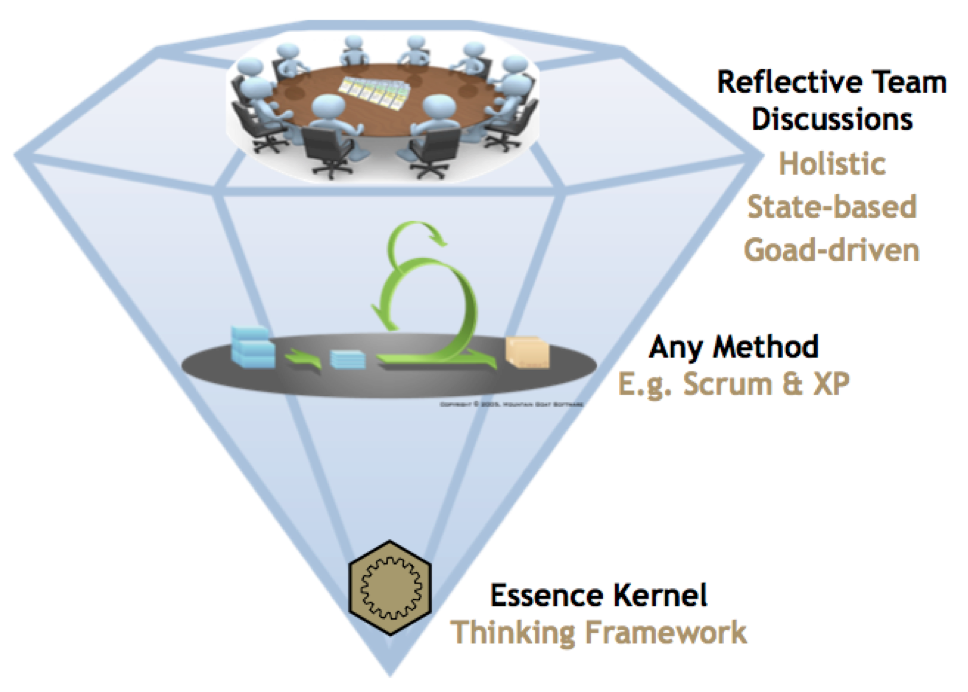
\includegraphics[width=3.4in]{reflection_meeting_images/EssenceDiamondEffect.png}
\caption{ Essence kernel's diamond effect}
\label{EssenceDiamondEffect}
\end{figure}

\textbf{Method-Agnostic}. The team decides what to do to reach the goals set by the target states. The team has the flexibility to leverage any software development method or set of practices that best suit their needs. This is illustrated in Figure \ref{EssenceDiamondEffect} with the Essence kernel's \quotes{diamond effect,} where the kernel alphas \quotes{radiate} to enable reflective discussions touching the many facets of the project throughout its lifecycle, independently of the software development method adopted by the team.

In conclusion, Essence supports team reflection by generating reflective team discussions through a thinking framework that is holistic, state-based, goal-driven, and method-agnostic. The teams benefit from stepping back and assessing the project holistically throughout its lifecycle. The goals set by the alpha state checklists lead the team to address critical aspects of the project that have been neglected. These aspects go beyond technology by including elements like \textbf{Team}, \textbf{Way of Working}, or \textbf{Stakeholders}.

\textbf{Research Question}: How does Essence reflection meetings compare to other types of reflection meetings?

Essence reflection meetings follow a state-based approach, with states covering the entire project lifecycle. Consequently, Essence reflection meetings are most effective if conducted on a regular basis throughout the entire project lifecycle. Therefore, Essence reflection meetings are not comparable to post-mortems or project retrospectives that are conducted only once at the end of the project (or release). Essence reflection meetings could be compared to Agile retrospectives \cite{Derby2006, KuaRetrospectiveHandbook}, because they are also conducted throughout the project lifecycle, typically at the end of each iteration or Sprint.

In this section we are comparing Agile retrospectives and Essence reflection meetings in terms of purpose, frequency, duration, structure, content, outcome, and facilitation concerns.

\textbf{Purpose}. The goal of an Agile retrospective is for the team to contemplate what worked and did not work during the last iteration in order to adapt the methods and teamwork moving forward. The focus is mostly on the past. The goal of an Essence reflection is for the team to consider various project dimensions in order to bring the whole project towards a higher state. The focus is mostly on the future.
  
\textbf{Frequency}. Both Agile retrospectives and Essence reflections can be conducted at the end of an iteration or Sprint, or at other intervals defined by the project team. During our field study, each team generally met on a weekly basis. We recommend frequent sessions early in the project when many issues arise. Later on, once a team becomes a high-performing team producing high quality outcome, the team needs less support and the frequency of the sessions could decrease.

\textbf{Duration}. Both Agile retrospectives and Essence reflections can be time boxed to a short session ranging from 30 minutes to a few hours. During our field study, each team generally met for a 30- minute session. We recommend adjusting the duration based on the team size and any other known parameters that might influence the length of the conversations, like team dynamic, issues and uncertainty, or session frequency.

\textbf{Structure}. While facilitators may run Agile retrospectives differently, many adopt a structure similar to the one proposed by Derby and Larsen in \cite{Derby2006}. Derby and Larsen generalize the stages of Agile retrospectives as: (1) Set the stage, (2) Gather data, (3) Generate insights, (4) Decide what to do, and (5) Close the retrospective. Even though Agile retrospectives and Essence reflections have a different structure, there are some similarities. During an Essence reflection meeting, the team repeats the key steps of gathering of data, generation of insights, and deciding what to do for each alpha. With the Essence kernel's seven alphas, this produces seven focused passes through the Agile retrospective stages. This structure is illustrated in Table \ref{ReflectionMeetingStructure}.

\begin{table}[t]
\renewcommand{\arraystretch}{1.5}
\centering
\caption{Essence reflection meeting structure}
\label{ReflectionMeetingStructure}
\begin{tabular}{p{3in}}
\hline
\textbf{Set the stage} (done informally) \\
\textit{For each alpha}:
  \begin{itemize}
  \item \textbf{Gather data (alpha states)} 
  
   Discuss alpha-related work since last session
   and agree on current and target states
  
  \item \textbf{Generate insights}

  Understand \textit{why} the target state is not achieved
  
  \item \textbf{Decide what to do}
  
  Set some goals to reach the target state 
  and agree on how to reach the goals

  \end{itemize}
    
\textbf{Close the retrospective} (done informally) \\
\hline
\end{tabular}
\end{table}


\textbf{Content}. One difference between Agile retrospectives and Essence reflections relates to the elicitation of topics to be covered during a session. During Agile retrospectives the topics discussed are elicited by the participants, while during Essence reflections the topics are determined by the alphas and their corresponding checklists. Issues emerge once the related alphas are covered. As a consequence, Agile retrospectives tend to focus on known issues while Essence reflections tend to make unknown issues apparent by covering the project holistically and reminding participants of \participantQuote{critical areas that are sometimes neglected.}

\textbf{Outcome}. Both Agile retrospectives and Essence reflections result in a small number of work items to be addressed, ideally before the next session. During an Agile retrospective, participants typically generate many possible work items that are prioritized and then limited to a few high value items to be addressed during the next iteration. During our field study, an average of 5 work items were generated per session. The identified work items were added to the team's work item list or backlog, and fed into the next planning activity when applicable.

\textbf{Facilitation}. Both Agile retrospectives and Essence reflections benefit from being conducted by an experienced and neutral facilitator. While this is often recommended for Agile retrospectives \cite{KuaRetrospectiveHandbook}, the need for a facilitator is reduced with Essence reflections as the Essence alphas and their checklists guide the discussions. A facilitator is only required during the initial sessions for training purposes. Similarly, it is generally recommended to prepare for Agile retrospectives ahead of time \cite{Derby2006, KuaRetrospectiveHandbook}. Essence reflection meetings might require the facilitator to print the cards ahead of time. We are currently leveraging an open source tool (available at http://essence.sv.cmu.edu) developed internally that provides digital cards, hence freeing us from any preparation. With such a tool, Essence reflection meetings are conducted very effectively with geographically distributed teams.

In conclusion, Essence reflection meetings could be compared to Agile retrospectives. Despite similarities between the two approaches, there are some key differences in terms of purpose and content. While Agile retrospectives aim at inspecting the last iteration in order to adapt the methods and teamwork (with a focus on the past), Essence reflections aim at considering various project dimensions in order to bring the whole project towards a higher state (with a focus on the future). While most styles of Agile retrospectives tend to focus on known issues, Essence reflections tend to make unknown issues apparent by covering the project holistically and reminding participants of critical areas that might be overlooked. These differences make Essence reflections and Agile retrospectives complementary. This is illustrated by the following student quote: \participantQuote{Though the team was holding retrospectives every week already, having Essence discussions be a part of it allowed the team to touch on important aspects of the project; aspects which would otherwise be ignored.}

\section {Conclusion}
Essence reflections are valuable and complementary to Agile retrospectives. Facilitators and project teams might want to leverage both. For instance, one might decide to conduct regular Essence reflection meetings during project initiation when the monitoring and steering mechanisms are the most effective \cite{ICSE2014}, then alternate between Essence reflections and other styles of Agile retrospectives. The value added by Essence reflections is to surface unknown issues, help monitor and steer the project towards a higher state, and prevent retrospectives from being repetitive by varying styles.

The results presented in this paper are limited to Essence reflection meetings with a facilitator. More research is necessary to assess the meetings' effectiveness without facilitators. Following the field study, we have been observing eight additional practicum teams. Our observations are consistent with the ones presented in the paper. We continue to collect data to evaluate the SEMAT Essence's framework with a focus on both effectiveness of the approach and accuracy of the model.

\begin{table*}[t]
\caption{How Essence is used in practice by a student team}
\centering
\begin{tabular}{l|l}
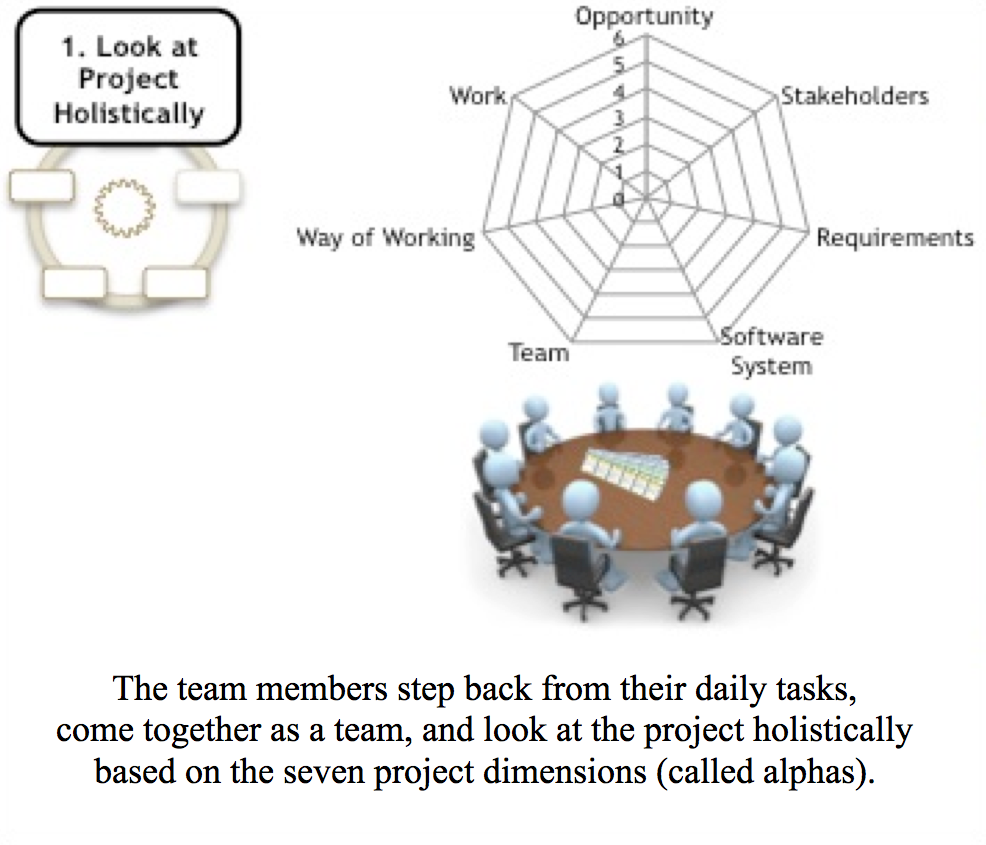
\includegraphics[width=3.2in]{reflection_meeting_images/EssenceMeetingStep1.png} & 
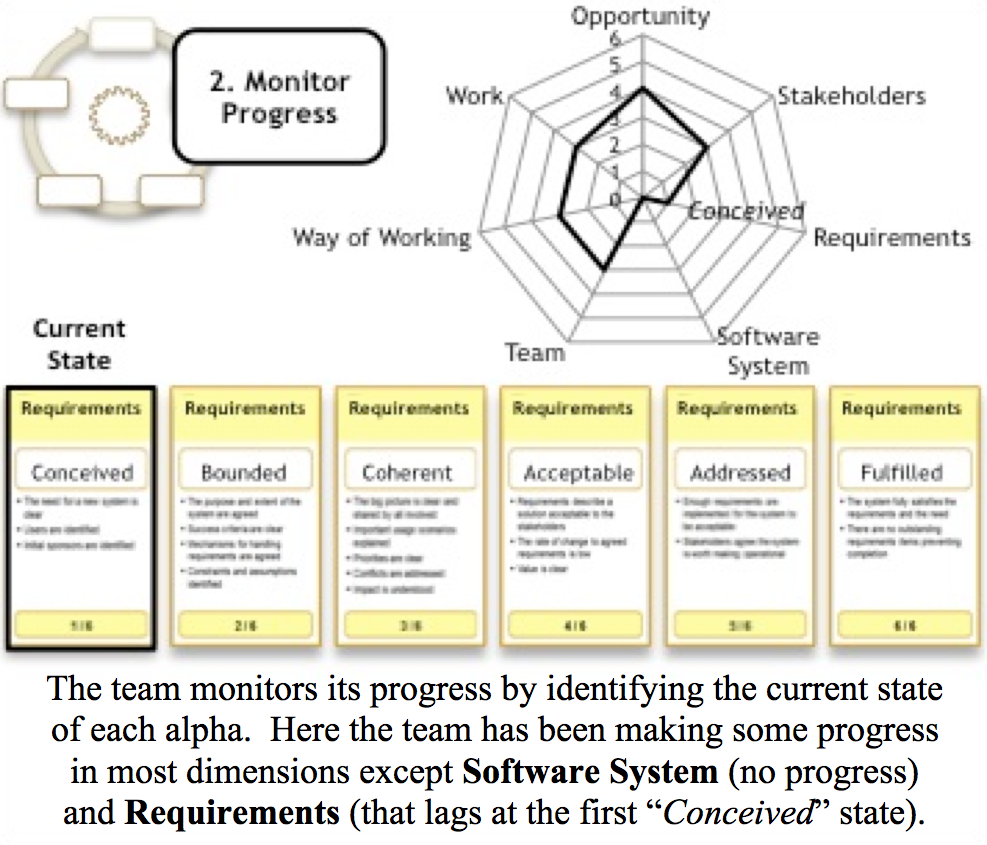
\includegraphics[width=3.2in]{reflection_meeting_images/EssenceMeetingStep2.png} \\
\hline
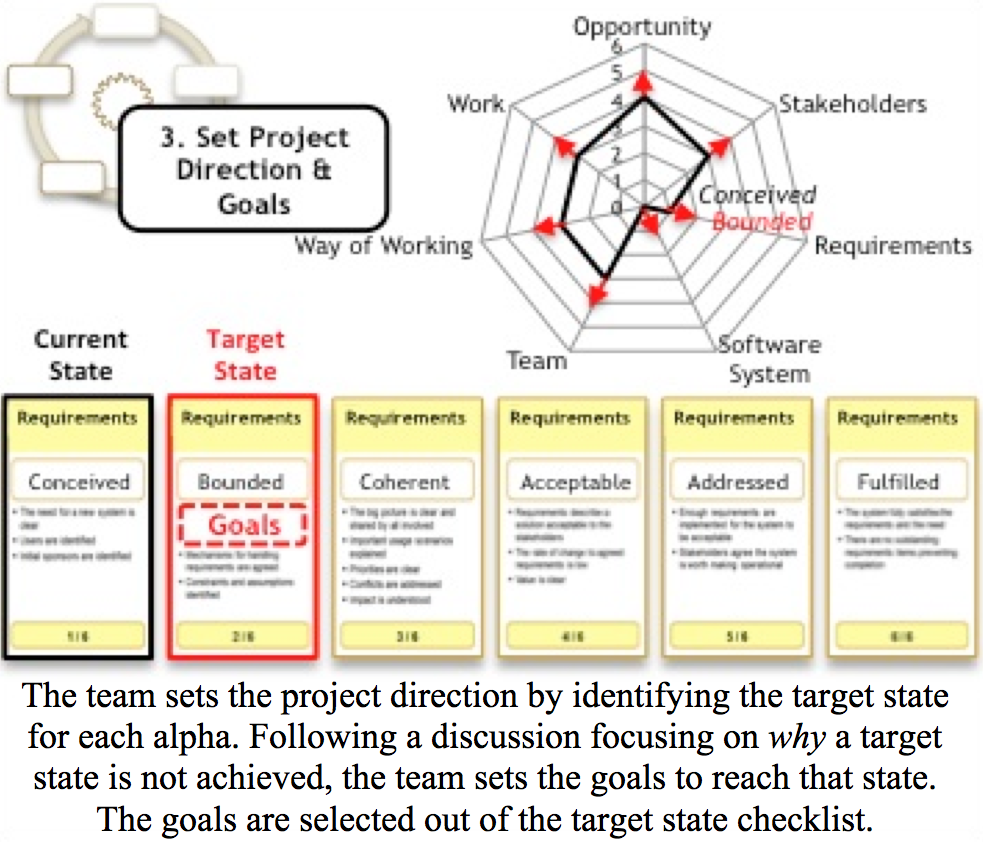
\includegraphics[width=3.2in]{reflection_meeting_images/EssenceMeetingStep3.png} &
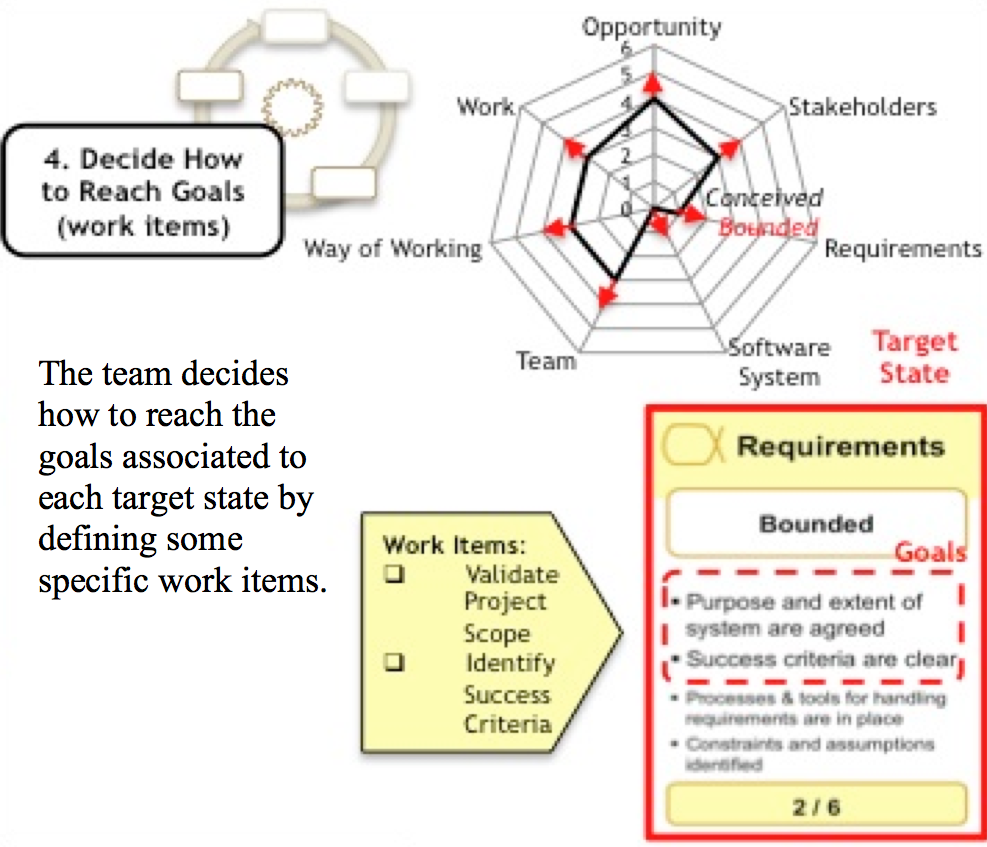
\includegraphics[width=3.2in]{reflection_meeting_images/EssenceMeetingStep4.png} \\
\hline
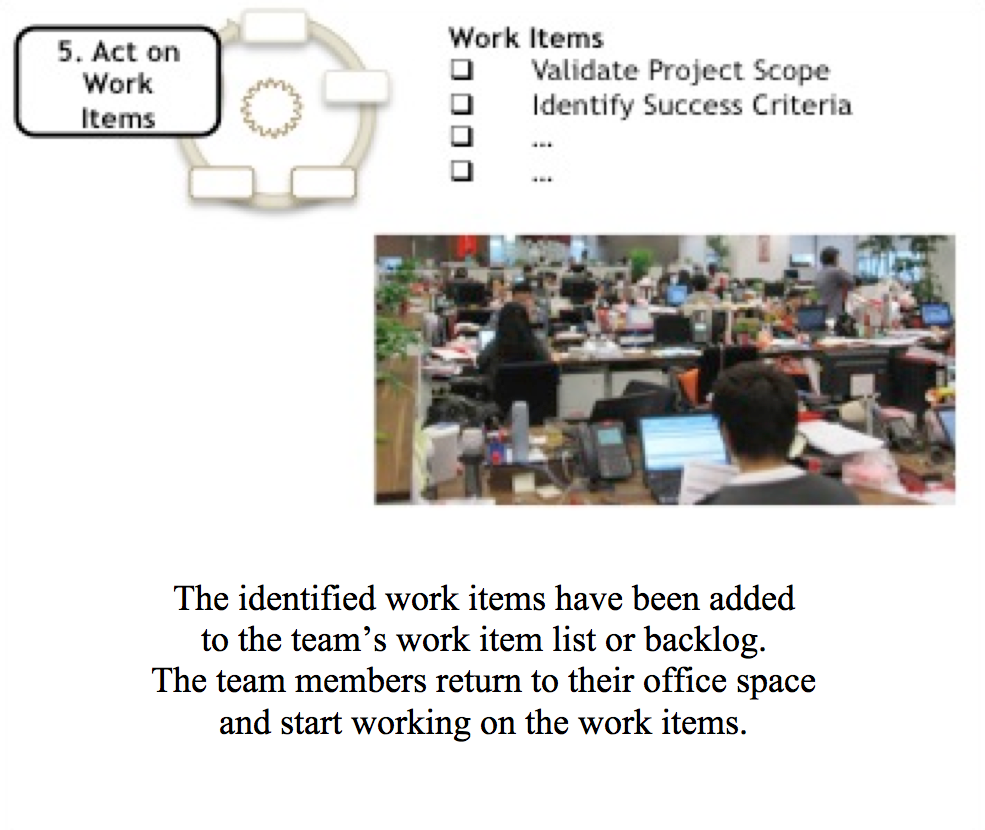
\includegraphics[width=3.2in]{reflection_meeting_images/EssenceMeetingStep5.png} &
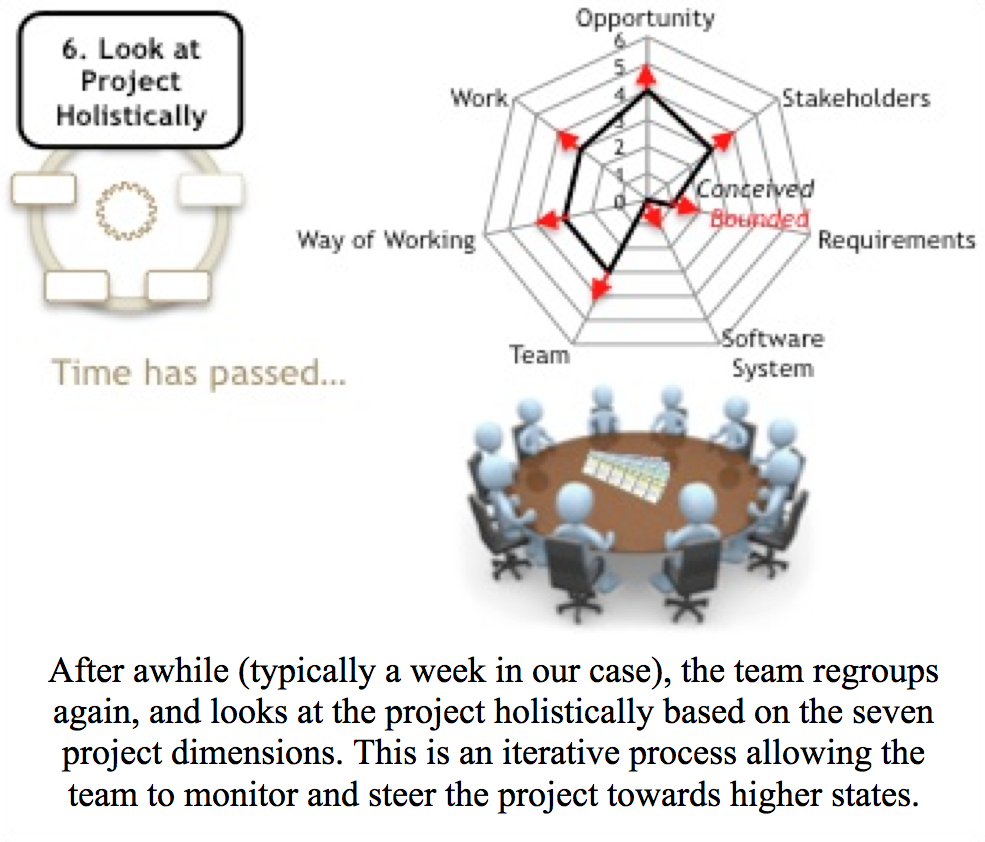
\includegraphics[width=3.2in]{reflection_meeting_images/EssenceMeetingStep6.png} \\
\end{tabular}
\label{EssenceReflectionMeetings}
\end{table*}
% \chapter{Essence Steering}

\section{Abstract}
At Carnegie Mellon University in Silicon Valley, the graduate master program ends with a practicum project during which students serve as software engineering consultants for an industry client. In this context, students are challenged to demonstrate their ability to work on self-managing and self-organizing teams. This paper presents a field study of the Software Engineering Method and Theory (SEMAT) Essence framework. The objective is to evaluate the effectiveness of the Essence's novel state-based monitoring and goal-driven steering approach provided by the Essence kernel alphas and their states. The researchers conducted the study on seven graduate master student teams applying the approach throughout their practicum projects. The research methodology involves weekly observation and recording of each team's state progression and collecting students' reflection on the application of the approach. The main result validates that the approach provides student teams with a holistic, lightweight, non-prescriptive and method-agnostic way to monitor progress and steer projects, as well as an effective structure for team reflection and risk management. The paper also validates that the Essence kernel provides an effective mechanism for monitoring and steering work common to most student software projects. This includes the work done during project initiation as well as the work done at the project or release level. Support for technical work should come from additional practices added on top of the kernel, or by extending or altering the kernel definition. The conclusion is that the approach enables students to learn to steer projects effectively by addressing the various dimensions of software engineering. Hence the approach could be leveraged in software engineering education.

\section{Introduction}

This paper presents the results of a field study of the Software Engineering Method and Theory (SEMAT) Essence framework \cite{SEMATKernel, EssenceBook} investigating the Essence kernels' novel approach to monitoring and steering software development projects. One of the promises of the approach lies in its potential ability to monitor any type of project holistically based on universal project states and steer these projects based on universal goals, hence making the monitoring and steering mechanisms independent from the method (such as Scrum \cite{AgileProjectManagement} and XP \cite{BeckExtremeProgramming2000}) or set of practices adopted by the project team.

We are interested in understanding the strengths and weaknesses of Essence by gaining experience of using the approach on real projects. We conducted a field study involving seven co-located and distributed student teams working on industrial projects. These students finish their graduate program with a project course at Carnegie Mellon University in Silicon Valley in the context of the Master of Science in Software Engineering program. During the project each student has the opportunity to apply the software engineering skills acquired throughout the program to solve a real industry problem. Monitoring and steering projects with the Essence kernel allows the researchers to identify where value is added for an educational program. Student team projects serve as a possible metaphor for newly formed industry team projects; the value added for a student team could transfer to an industry team.

As faculty, we allow teams to be self-organizing and responsible for their decisions, yet at the same time expect them to incorporate generally accepted software engineering practices, and demonstrate the ability to effectively steer their project. Each team manages its own project with minimal faculty supervision. In the past, the faculty observed that with minimal supervision some teams revert to old habits \cite{BareissTransferable}. As soon as the starting bell sounds, they can act as racetrack horses running towards the finish line with blinders, ignoring what they have learned in class and without concerns for software engineering discipline. The new freedom and the chance to write code for a client lead them to focus mostly on implementation and therefore to adopting a suboptimal way of working.

Our research hypothesis contends that Essence's monitoring and steering approach provides a lightweight framework for students to look at their project holistically, helping them to address various project dimensions beyond implementation. We stipulate that the framework acts as a routine reminder about applicable software engineering practices covered in previous courses, and this without being prescriptive and while being method agnostic. For instance, by using this technique, we expect students to think about involving stakeholders, improving the team's way of working, and demonstrating that the software system has the desired quality characteristics.

This paper reviews SEMAT's Essence framework and kernel, describes the field study planning and execution, reports on the analysis and interpretation of the field study data, recommends effective practices for introduction of Essence to a software engineering curriculum, and summarizes the conclusions.

\section{SEMAT ESSENCE OVERVIEW}
In 2009, Ivar Jacobson, Bertrand Meyer, and Richard Soley started work on the \quotes{Software Engineering Method and Theory} (SEMAT) with the goal of \quotes{re-founding software engineering as a rigorous discipline} \cite{JacobsonCallForAction}. While many software engineering principles, techniques, practices and methods exist, the SEMAT founders' ambition is to create a general theory of software engineering and a unifying process framework. Out of their initiative has emerged the SEMAT Essence language and kernel, which became an Object Management Group (OMG) beta standard in 2013.

The core idea of Essence is that software projects exhibit universal behavior and transition through identifiable states as they progress. Essence groups these states together by different software engineering aspects or dimensions called \quotes{alphas.} Essence identifies seven alphas as core to every software engineering project: \textbf{Stakeholders}, \textbf{Opportunity}, \textbf{Requirements}, \textbf{Software System}, \textbf{Team}, \textbf{Way of Working}, and \textbf{Work}. These seven alphas serve as the Essence kernel as illustrated in Figure \ref{EssenceKernel}.

\begin{figure}[h]
\centering
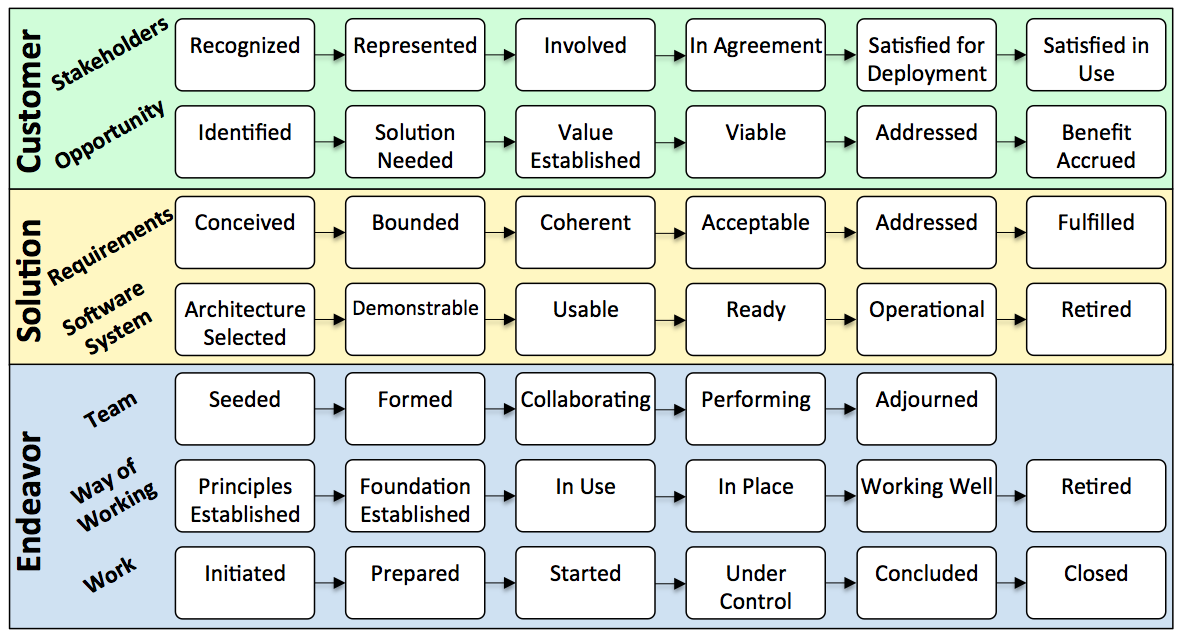
\includegraphics[width=3.30in]{project_steering_images/EssenceKernel.png}
\caption{Essence kernel alphas and their states }
\label{EssenceKernel}
\end{figure}

Each alpha progresses through a number of states during the project lifecycle. For example, the \textbf{Stakeholders} alpha progresses through the states \textit{Recognized}, \textit{Represented}, \textit{Involved}, \textit{In Agreement}, \textit{Satisfied for Deployment}, and \textit{Satisfied in Use}. Each state includes a checklist to help determine if the project has achieved that state. Each checklist item provides a goal to be reached in order to progress to that state.

Despite the sequential definition of the states for each alpha, in practice, projects could fall back to previous states. Similarly, in some circumstances, it might make sense for a project to achieve a number of states simultaneously within a given alpha.

The SEMAT vision is also to create a library of practices described using the Essence language and sitting on top of the Essence kernel. Practices would be composed to become specific methods addressing specific project or organization needs. Practices would help a team identify how to progress their project from one state to the next.

In The Essence of Software Engineering \cite{EssenceBook}, the authors identify three separate applications of Essence: 1) project monitoring and steering, 2) determining when to green light projects, and 3) describing workflow through an organizational structure. This paper focuses mostly on the first application, project monitoring and steering, where a team assesses its current project state in each of the alphas and identifies possible actions to help transition from the current state to the next target state.

\section{Field Study Description}
\label{Field Study Description}

The study focuses on understanding what value do project teams receive from following the SEMAT Essence's monitoring and steering approach provided by the kernel alphas and their states. Essence was introduced to master students at the beginning of their practicum projects. The students had no prior knowledge of Essence.

Using the goal template from GQM \cite{GQM}, our research goal is to:

\begin{table}[h]
\renewcommand{\arraystretch}{1.3}
\centering
\begin{tabular}{|p{1.20in}|p{1.90in}|}
\hline
\textbf{Analyze} & SEMAT Essence's monitoring and steering approach provided by the kernel alphas and their states \\ \hline
\textbf{for the purpose of} & evaluation \\ \hline
\textbf{with respect to its} & effectiveness \\ \hline
\textbf{from the point of view of the} & project team, educator, and researcher \\ \hline
\textbf{in the context of} & the software engineering practicum graduate course at Carnegie Mellon University. \\
\hline
\end{tabular}
\end{table}
 
This paper decomposes this goal into the following questions:

\textbf{Research Question 1}: Does the SEMAT Essence's monitoring and steering approach provide value to the project team?

\textbf{Research Question 2}: How does the approach provide value to the project team?

\textbf{Research Question 3}: When in the project lifecycle does the approach add value?

\textbf{Research Question 4}: What are the limitations to the approach's effectiveness?

The first section below describes the context of each project involved during the field study. The second section presents how Essence was introduced to the teams, either incrementally or using a workshop approach. The final section describes how the teams have been leveraging Essence during the remaining of their project.

\subsection{Practicum Projects' Context}


\begin{table*}[t]
\centering
\renewcommand{\arraystretch}{1.4}
\caption{Practicum projects' context}
\label{PracticumProjectsContext}
% \begin{tabular}{|p{0.6in}|p{1.1in}|p{1.1in}|}
\begin{tabular}{|p{0.75in}|p{1.05in}|p{0.3in}|p{1.05in}|p{0.7in}|p{2.3in}|}
\hline
\textbf{Team Name} &
\textbf{Industry Project} &
\textbf{Team Size} &
\textbf{Team Distribution} & 
\textbf{Average Work Experience} &
\textbf{Technical Complexity} \\
\hline
\hline
\multicolumn{6}{|l|}{\textbf{First Pilot Projects}} \\ 
\hline

Distributed-1 & 
Rendering of audio streams for accessibility purpose &
3 &
Distributed within same time zone &
10 years &
Integration with legacy code on a single platform involving C, HTML5 and open-source technology. \\
\hline

Distributed-2 & 
Access and preservation of electronic journals & 
4 & 
Distributed across 2 time zones & 
6 years &
Integration with legacy code on a single platform involving Java, MongoDB, Apache Jena and open-source technology. \\
 \hline

Distributed-3 & 
Survivable social network & 
4 & 
Distributed across 2 time zones & 
8 years &
Multi-platform involving Ruby on Rails, Javascript, jQuery Mobile. Embedded system constraints. \\
\hline

\multicolumn{6}{|l|}{\textbf{Second Pilot Projects}} \\ 
\hline

Co-located-1 & 
Electric vehicle fleet management & 
2 & 
Co-located & 
3 years & 
Green-field development involving Query, Node.js and MongoDB. Integration with Rest APIs for two vehicle brands. \\
\hline

Co-located-2 & 
Sonification of financial trading information & 
4 & 
Co-located & 
3 years & 
Integrates with third party APIs (Yahoo! and Google Finance). Involves Objective C, Ruby on Rails, iOS, Google App Engine and Python. Requires financial knowledge. Has a special focus on user experience. \\
\hline

Co-located-3 & 
Mobile performance testing & 
3 & 
Co-located & 
4 years & 
Xcode, Instruments, Eclipse, iOS 6.0, Android 4.2, jQuery Mobile, HTML5, Benchmark.js, Appception, Pivotal tracker, Redmine, GitHub, RubyMine, Rails 3.2, Ruby 1.9.2. Heroku, Amazon EC2, HighCharts.js, CSS3, Cordova \\
\hline

Co-located-4 & 
Virtual sensors definition and management & 
5 & 
Co-located & 
5 years & 
Multi-platforms involving HTML5, Javascript and j2ee. \\
\hline

\end{tabular}
\end{table*}


The authors introduced Essence to seven student teams: three geographically distributed student teams, referred as Distributed-1 to Distributed-3 for the purpose of this paper, and four co-located student teams, referred as Co-located-1 to Co-located-4. As shown in Table \ref{PracticumProjectsContext}, each team worked on creating or evolving a software solution for a different client, like an electric car fleet management system or a survivable social network. By design, the projects had a medium to high level of technical complexity, as they often involved multiple technologies or platforms or integrate with legacy systems.

The geographically distributed, part time students were working professionals with an average of eight years of development experience. Their practicum projects ran for 15 weeks, during which each student dedicated about 20 hours per week to the project. They worked in small teams of three to four members distributed across one or two time zones.

The co-located, full time students were at the beginning of their career with an average of four years of development experience. Their practicum projects ran for 12 weeks, during which each student dedicated about 20 hours per week to the project. They worked in co-located teams of two to five members.

The course syllabus imposed a few milestones and deliverables (like roadmap, statement of work, reflection report, and working software), with potential additional requests coming from the client. Teams determined their own software development approach. Most students had a reasonable knowledge of a diverse set of generally accepted software engineering practices, and the ability to execute these practices somehow effectively. All projects adopted an iterative lifecycle.

Even though the student population was quite diverse in terms of origin and culture, by the time the students started their practicum project they were immersed in the North American culture for at least eight months.

Table \ref{PracticumProjectsContext} summarizes the context of each practicum project in terms of the following dimensions \cite{AmblerDAD, BoehmBalancingAgilityAndDiscipline, KruchtenContextualizingAgile}: team size, team distribution, average work experience, and technical complexity.

Essence was introduced to the geographically distributed teams in the context of a first set of pilot projects, and to the co-located teams in the context of a second set of pilot projects

\subsection{Introducing Essence on Practicum Projects}
\subsubsection{First Pilot Projects - Incremental Approach}
In the Spring 2013 semester, the authors introduced the SEMAT Essence framework to three geographically distributed student teams at the beginning of the project. Because first impressions are critical for adoption, and because the researchers were uncertain of the value provided by Essence, we made the decision of introducing the framework with minimum overhead to avoid adoption resistance and minimize potential waste.

We briefly introduced Essence to all students using a slide presentation of about 20 minutes. Since the teams were distributed, a set of physical Essence cards was sent to each student, and a digital Essence board was created using Google Drawing (see Figure \ref{DigitalEssenceBoard}). The digital board included one row for each of the seven alphas in the Kernel. Each row contained the sequence of states that the alpha progresses through during the project lifecycle.

\begin{figure}[t]
\centering
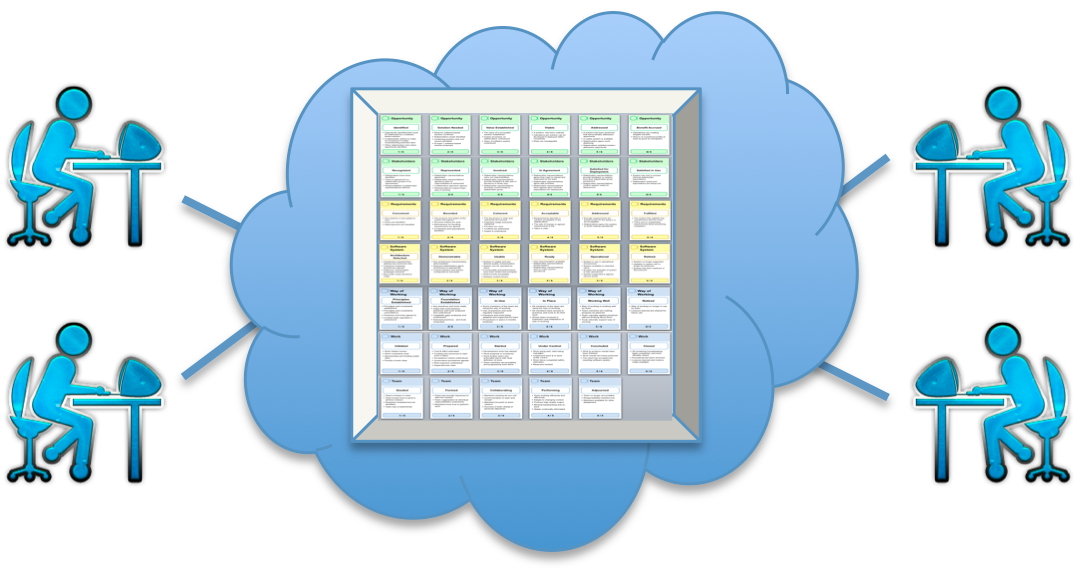
\includegraphics[width=3.40in]{project_steering_images/DigitalEssenceBoard.png}
\caption{Digital Essence board}
\label{DigitalEssenceBoard}
\end{figure}

After the initial presentation, the alphas were introduced incrementally over a number of 30 minute sessions, in order to make the experience as lightweight as possible. Each team met individually with a faculty and applied Essence on their practicum project. As an example, here is what happened with one team over a one-month period:

\underline{\textbf{Session 1}}: The two \quotes{customer} alphas, \textbf{Opportunity} and \textbf{Stakeholder}, were introduced. The main reason for introducing these two alphas first, was simply because it generally makes sense to have a discussion around the opportunity and stakeholders early in the project and before drilling down into the details of the solution and endeavor.

\underline{\textbf{Session 2}}: After updating the progress made for the previously introduced alphas, one \quotes{solution} alpha, \textbf{Requirements}, was introduced. The rationale for introducing this alpha was based on a pain point, as the team was expressing concerns around the client's expectations and hence needed to have a discussion around project scope and success criteria in relation with the \textbf{Requirements} alpha.

\underline{\textbf{Session 3}}: After updating the progress made for previously introduced alphas, two \quotes{endeavor} alphas, \textbf{Team} and \textbf{Way of Working}, were introduced based on additional pain points. Indeed the team was having some communication issues and hence needed to have a discussion around team collaboration and way of working.

\underline{\textbf{Session 4}}: After updating the progress made for previously introduced alphas, the remaining alphas were introduced for completeness: \textbf{Software System} and \textbf{Work}.

For each alpha, the team identified the current state, the target state, and any work items necessary to progress from the current to the target state. The identification of the current and target states was done through an informal discussion until the team reached an agreement.

To continue the example above, during the second session the team identified \textit{Conceived} as the current state for the \textbf{Requirements} alpha and \textit{Bounded} for the target state. Indeed all the items on the \textit{Conceived} checklist were satisfied while a few items on the Bounded checklist were not satisfied. In order to achieve \textit{Bounded}, the team first needed to define the project scope and clarify the success criteria with the client, as illustrated in Figure \ref{WorkItems}. The work items were dealt with right away or added to the team's work item list or backlog.

\begin{figure}[h]
\centering
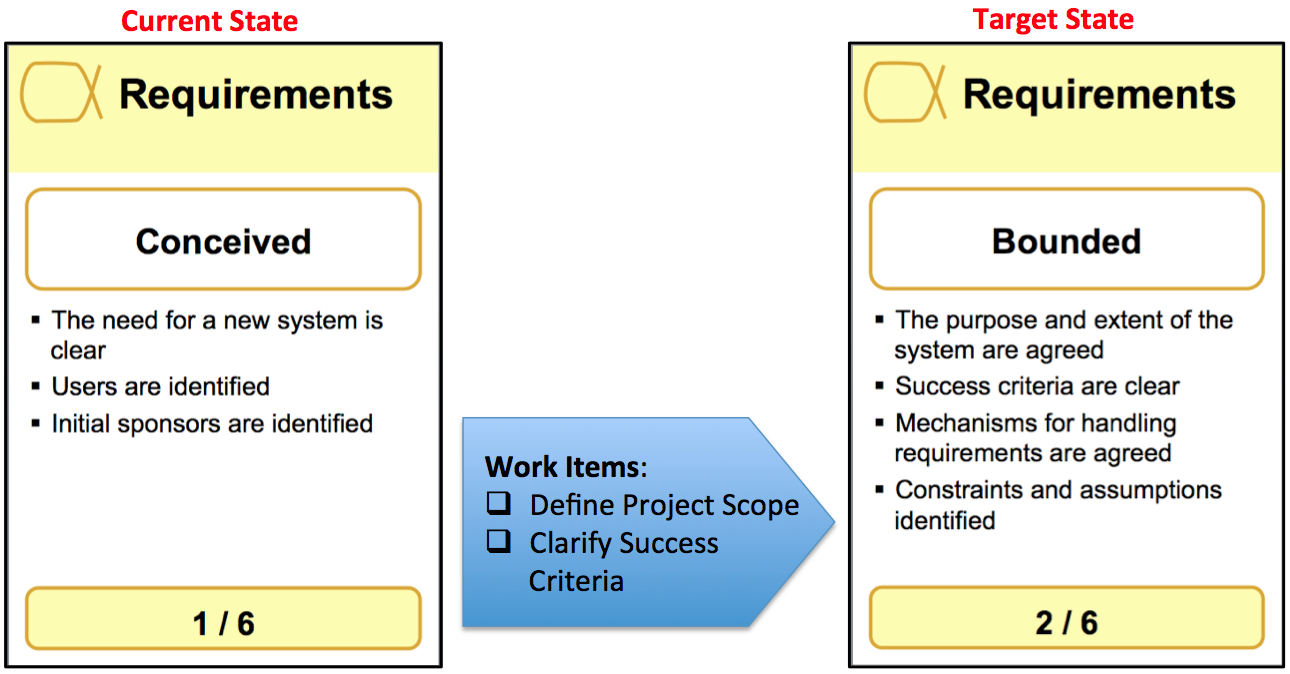
\includegraphics[width=3.30in]{project_steering_images/WorkItems.png}
\caption{Work items to reach the Bounded state}
\label{WorkItems}
\end{figure}

With mentoring from faculty, Essence was introduced to the geographically distributed teams using the incremental approach described above. For each team, and following the initial presentation of the Essence framework, four sessions of about 30 minutes long were necessary in order to introduce all the seven alphas incrementally. During each session, elements relevant to our study were jointly logged by students and faculty as described in Section \ref{UsingEssenceOnPracticumProjects} below.

\subsubsection{Second Pilot Projects - Workshop Approach}
In the Summer 2013 semester, Essence was introduced to four co-located teams at the beginning of the project. Based on our previous experience with the distributed students and armed with encouraging results (presented in Section \ref{FieldStudyAnalysis} below), we decided to speed-up the introduction process using a workshop approach. Our goal was to help the teams benefit from Essence as early as possible in the lifecycle.

The workshop was time-boxed to 90 minutes and included all students. It consisted of a general introduction of the Essence framework, the motivation for adopting the framework, together with exercises teaching each team how to apply the Essence's monitoring and steering approach on their own practicum project, one alpha at a time. Like in the first pilot projects and for the same reasons, the two green \quotes{customer} alphas, \textbf{Opportunity} and \textbf{Stakeholders}, were introduced first. Then, the remaining alphas (\textbf{Requirements}, \textbf{Software System}, \textbf{Team}, \textbf{Way of Working}, and \textbf{Work}) were introduced based on pain points when applicable, or in a random order otherwise. For each alpha, each team was tasked of identifying their project current state, target state, and any work items necessary to transition from the current to the target state. The identified work items were added to the team's work item list or backlog.

A couple of changes were introduced compared to the first pilot projects:

\begin{itemize}
    \item \textbf{Moving from physical cards to physical strips.} Handling a large set of cards could be a hassle. Therefore, we decided to create strips instead, as illustrated in Figure \ref{OneAlphaStrip}. For each alpha, one strip represents the typical sequence of states that the alpha progresses through during the project lifecycle. This way, we could easily provide the students with the information they needed to work on various alphas, one alpha at a time. Note that since the students were all physically present during the workshop, no digital boards were used.
    
    \item \textbf{Adoption of a poker game approach for state identification.} In order to remove anchoring bias, the informal way of identifying the current and target states was replaced with a \quotes{poker game} approach. In that context, each participant does a blind determination of their current state and all reveal their current state at the same time. In case of disagreement, the team discusses the different points of view until the participants reach an agreement. This technique is a simplification of Wideband Delphi \cite{StellmanAppliedPM} and agile estimation using Planning Poker \cite{GrenningPlanningPoker}, as the participants perform only one round of \quotes{estimation.} Just like Delphi and Planning Poker, the value is in the conversation, and allowing the team members to work through their different perspectives.
\end{itemize}

\begin{figure}[h]
\centering
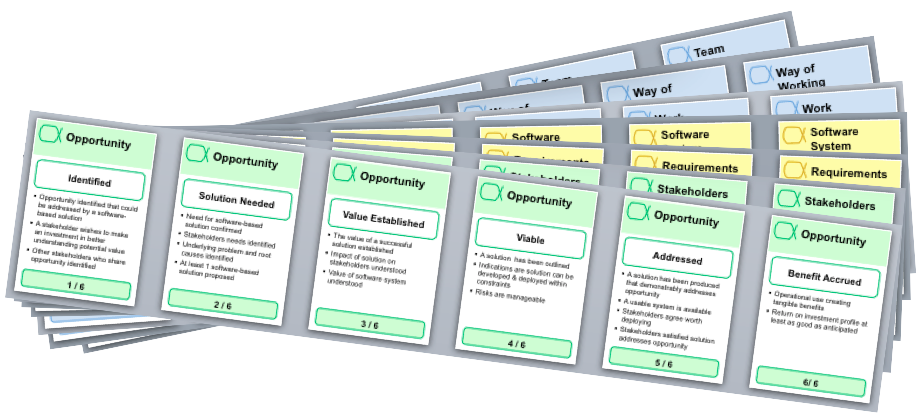
\includegraphics[width=3.30in]{project_steering_images/OneAlphaStrip.png}
\caption{One strip per alpha}
\label{OneAlphaStrip}
\end{figure}

Using the workshop approach described above, and with mentoring from faculty, Essence was introduced to the co-located teams over a 90 minutes session. On average, 10 minutes were necessary for a team to cover one alpha, and most teams were able to cover the seven alphas during the workshop. Students and faculty jointly logged elements relevant to our study as described in the following section.

\subsection{Using Essence on Practicum Projects}
\label{UsingEssenceOnPracticumProjects}
Once Essence was introduced, the teams were asked to continue leveraging the approach during the remainder of their project. Each team met on a regular basis (mostly weekly) for a 30 minutes session. During each session, the team reviewed most or all of the alphas. For each alpha, the team identified their project's current states following the poker game approach. The team would consider work items necessary to transition from the current state to the target state. Any new identified work items were added to the team's work item list or backlog. Teams were encouraged to act on their work items as soon as possible to accelerate their state progression

A faculty member was present to facilitate each session. Faculty involvement was kept at a minimum to limit influencing the steering of the project. The faculty's role was constrained to guiding the team through the application of the Essence monitoring and steering approach, and to validating the objectivity of the team's self-assessment of their project state. By listening to the team's discussions, and asking clarification questions as needed, the faculty gauged the project state. At times, this helped reduce the tendency of some teams to be overly pessimistic or optimistic about the project state.

For the purpose of the field study, progress and work items were recorded jointly by the students and faculty using the teams' Essence progress log, as shown in Table \ref{EssenceProgressLog}.

\begin{table*}[]
\centering
\caption{Essence progress log}
\renewcommand{\arraystretch}{1.4}
\label{EssenceProgressLog}
\begin{tabular}{|l|l|l|p{3.25in}|}
\hline
\multicolumn{4}{|l|}{Date:}                                         \\ \hline
\hline
Alpha           & Current State & Target State & Work Items / Notes \\
\hline
Stakeholders    &               &              &                    \\ \hline
Opportunity     &               &              &                    \\ \hline
Requirements    &               &              &                    \\ \hline
Software System &               &              &                    \\ \hline
Team            &               &              &                    \\ \hline
Way of Working  &               &              &                    \\ \hline
Work            &               &              &                    \\ \hline
\end{tabular}
\end{table*}

% \begin{figure}[h]
% \centering
% \includegraphics[width=3.30in]{project_steering_images/EssenceProgressLog.png}
% \caption{Essence progress log}
% \label{EssenceProgressLog}
% \end{figure}

The distributed students mostly used their digital Essence board, while the co-located teams used both digital Essence board and strips. Some students kept their strips handy and used them throughout the project lifecycle while others preferred to rely on the digital board.

At the end of the projects a survey was sent to the students, including the following questions:

\textbf{Survey Question 1}: What did you like the most about Essence? 

\textbf{Survey Question 2}: What did you like the least about Essence? 

\textbf{Survey Question 3}: In using Essence, did you adopt a practice that you wouldn't have? Or did you adopt it earlier than you would have without using Essence? (Please explain)

\textbf{Survey Question 4}: Was following the Essence approach worth your time? (Please explain why or why not)

\textbf{Survey Question 5}: Would you use Essence on your next project? (Please explain why or why not)

\textbf{Survey Question 6}: Anything else that we should know?

\section{FIELD STUDY ANALYSIS \& INTERPRETATION}
\label{FieldStudyAnalysis}
Our research questions relate to the value provided by the SEMAT Essence's monitoring and steering approach. The researchers measured the qualitative value based on students' feedback collected mostly during the weekly SEMAT sessions, course reflection reports, and final survey. The researchers measured the quantitative value based on alpha state progression as well as the number of work items generated during the weekly SEMAT sessions and allowing bringing the project to a higher state. Refer to Figure \ref{FieldStudyRowData} in the Appendix for the raw data collected on alpha state progression, and to Figure \ref{NewWorkItemsGenerated} under Research Question 3 for the number of work items generated by the approach per week.

\textbf{Research Question 1}: Does the SEMAT Essence's monitoring and steering approach provide value to the project team?

Our field study shows that students receive value from SEMAT Essence's monitoring and steering approach provided by the kernel alphas and their states. In our survey, 90\% of the students said that following the approach was worth their time (80\% of the students participated in the survey.) Similarly, 80\% said that they will use the approach on their next project.

By following the approach, project teams monitored their progression through the Essence states over time, as illustrated in Figure \ref{AlphaProgressionColocated4} for team Co-located-4. Every week this team generated on average 6 new work items during their SEMAT session, and then acted on these work items in order to bring the project to a higher state.

\begin{figure}[h]
\centering
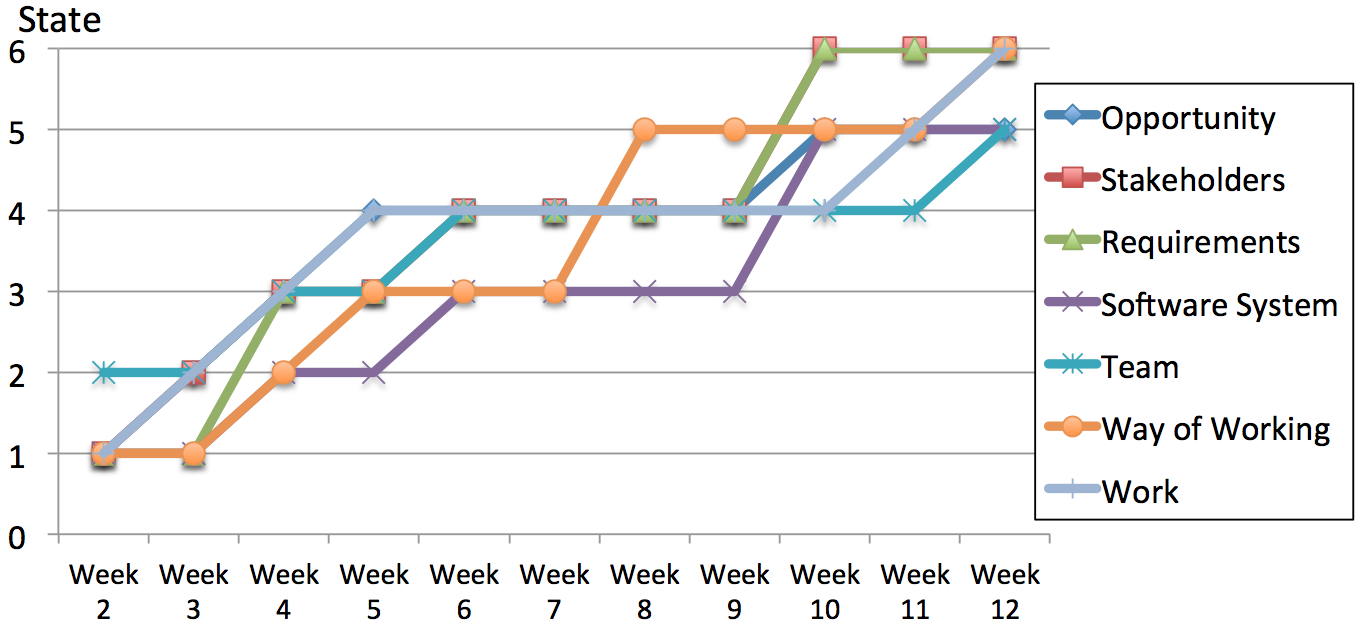
\includegraphics[width=3.30in]{project_steering_images/AlphaProgressionColocated4.png}
\caption{Alpha progression for team Co-located-4}
\label{AlphaProgressionColocated4}
\end{figure}


In conclusion, most students have a positive perception of this approach as it helps them make decisions allowing to move their project forward.

\textbf{Research Question 2}: How does SEMAT Essence's monitoring and steering approach provide value to the project team?

The benefits that a project team receives from SEMAT Essence's monitoring and steering approach come primarily from the discussions that occur when the team is covering the various alphas. The discussions enable the team to pause and assess the situation:

\begin{itemize}
    \item \textbf{The team steps back from its daily tasks and examines its project holistically.} One student noted: \participantQuote{Essence gives us a chance to step back and look at the project as a whole, from a bird's-eye view. There are aspects that we tend to ignore when focused on the technology. Essence is very useful, because it makes me think about these particular aspects.} Similarly, another student noted: \participantQuote{I like the fact that Essence provides a structured way of thinking about critical aspects of the project at different stages of the project. Without Essence, our team could have overlooked some of these aspects.} Stepping back and looking at the project holistically is a healthy exercise providing the distance and perspectives needed to understand a situation, reflect, and make decisions. When asked about what they like the most about Essence, most students mentioned reflection or retrospective. For instance one student noted: \participantQuote{Though the team was holding retrospectives every week already, having Essence discussions be a part of it allowed the team to touch on important aspects of the project.}
    
    \item \textbf{The team records progress accomplished and identifies what remains to be done.} When asked about what she liked the most about Essence, one student answered: \participantQuote{The choice of alphas: they seem to be exactly the right areas to monitor to promote the success of a software project.} The Essence mechanism for monitoring progress is illustrated in Figure \ref{ProjectStateDistributed3}. The chart shows the progress made by team Distributed-3 at week 5, compared to the practicum target state established by faculty. The team has been making good progress towards the target goal in most dimensions except \textbf{Software System} that lags at state 1 (\quotes{\textit{Architecture Selected}}). This situation served as a red flag and a reminder that the team needed to focus its effort on taking their software system to the next level. The approach was used as a similar risk management mechanism in other instances. When asked if he would use Essence on his next project, one student answered: \participantQuote{Yes, it 's great for team reflection and risk management.}
    
    \item \textbf{The team seeks guidance on what directions to take and identifies goals to transition to a higher project state.} Team Distributed-1 noted: \participantQuote{Essence gives us structure and direction.} Another student commented: \participantQuote{Essence is useful, as it gives you an agenda or checklist based on various dimensions (even though I was skeptical at first).} Essence provides a simple project steering mechanism. For each alpha, the identified target state provides the direction to take, and its checklist provides goals to reach. For instance and to continue the example above, during week 5 team Distributed-3 identified \quotes{\textit{Demonstrated}} as its target state for \textbf{Software System}, with a number of goals including demonstrating the key architecture characteristics, as illustrated in Figure \ref{ProjectStateDistributed3}.
    
    \item \textbf{The team decides what to do to reach the target goals. Once the team identifies the goals, the team members rely on their software engineering knowledge and experience to decide how to reach these goals.} Indeed, Essence does not prescribe the use of any existing method (like Scrum or XP) or set of practices or work items. Instead, the team has the flexibility to leverage any method or set of practices that best suit their needs, and decide what work items to perform to reach the goals set by the target state. As a consequence, our seven practicum teams were able to leverage Essence even though they all used a different set of software engineering practices. When asked if he would use Essence on his next project, one student answered: \participantQuote{Yes, especially with a project team that is not used to the same software engineering process. In that instance Essence is a backdrop at the basis of the communication about all the considerations for the success of the project.} Another student added: \participantQuote{It is simple, lightweight and useful.}
\end{itemize}

\begin{figure}[t]
\centering
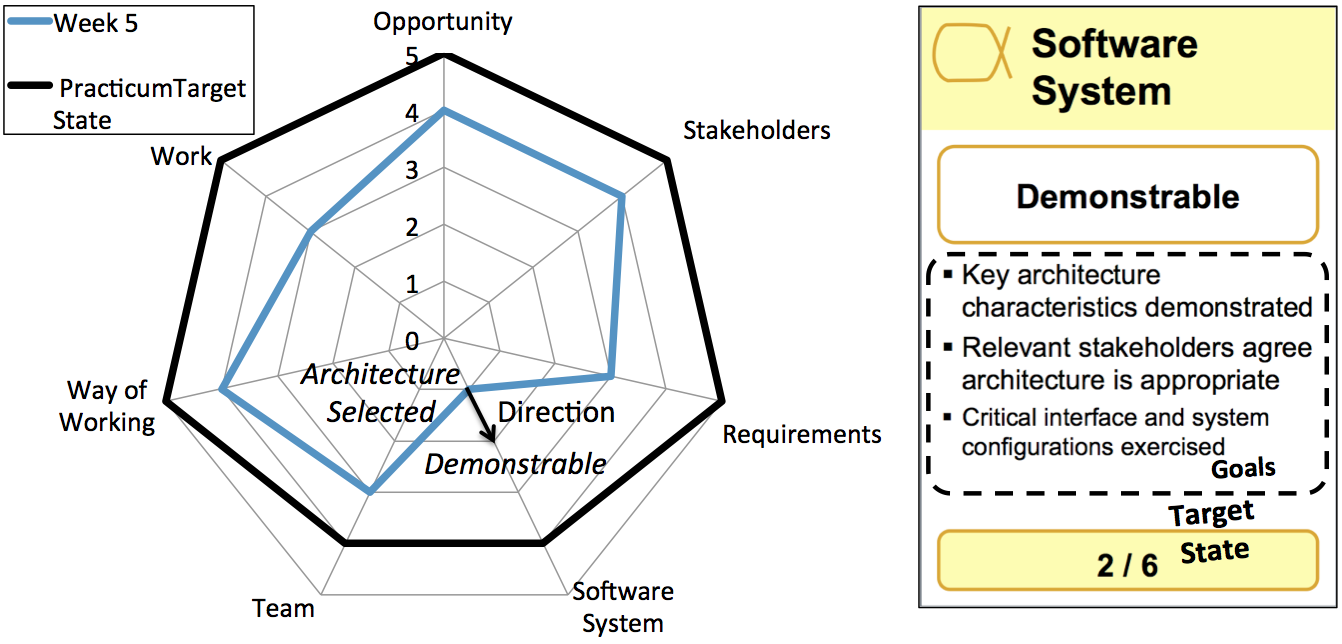
\includegraphics[width=3.30in]{project_steering_images/ProjectStateDistributed3.png}
\caption{Project state for team Distributed-3 at week 5, with direction and goals for Software System}
\label{ProjectStateDistributed3}
\end{figure}


The team accelerates its state progression by acting on its work items as soon as possible and iterating through the steps described above. Figure \ref{EssenceMonitoringLoop} illustrates this iterative process.

\begin{figure}[t]
\centering
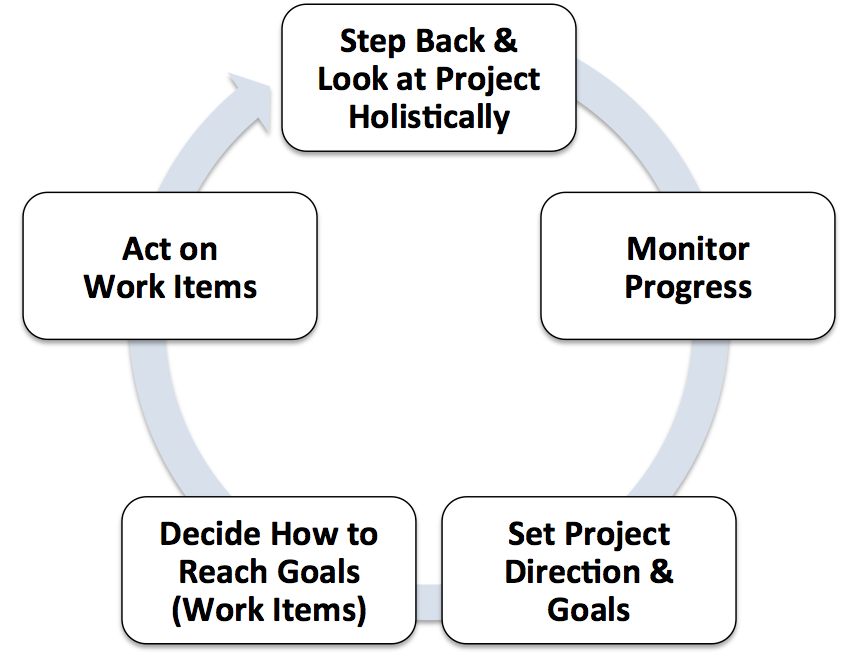
\includegraphics[width=3.30in]{project_steering_images/EssenceMonitoringLoop.png}
\caption{Essence monitoring and steering loop}
\label{EssenceMonitoringLoop}
\end{figure}

In answer to our second research question, the approach adds value by providing the project team with a holistic view of the project, a mechanism for monitoring progress and steering projects, as well as an effective structure for team reflection and risk management. This is provided in a simple, lightweight, non-prescriptive and method-agnostic fashion.

\textbf{Research Question 3}: When in the project lifecycle does the SEMAT Essence's monitoring and steering approach add value?
The value that the teams receive from SEMAT Essence's monitoring and steering approach varies over the project lifecycle. Our study shows that most value is generated at the beginning of the project and that it decreases thereafter. Here are some illustrating quotes:
\begin{itemize}
    \item When asked if following the Essence approach was worth their time, 20\% of the students who answered yes to the question qualified their answers as follows: \participantQuote{Yes, it helped us at the beginning of the project}, or \participantQuote{Yes, it was worth my time in the first half of the project.}
    
    \item Among the students who mentioned that they would use Essence on their next project, one qualified her answer as follows: \participantQuote{Yes, but only at the beginning of the project.}
    
    \item When asked what he liked the least about Essence, one student answered: \participantQuote{Essence lost value once the project settled because we dead ended on a set of cards.} Another student added: \participantQuote{Essence is useful in the planning stages. Later on its usefulness is dying down. If you spend multiple weeks on one card, then spending time looking at it is less helpful.} This opinion is shared by about 50\% of the students.
    
    \item The faculty in charge of the practicum course, and who has taught the course for 10 years, noted: \participantQuote{Compared to previous years, I see a much better early project organization with lot less floundering. I hope that we keep using Essence in the future. We should definitely keep it at the beginning of the projects.}
\end{itemize}

The alpha progression of team Co-located-3 illustrates the decrease in value, as seen in Figure \ref{AlphaProgressionColocated3}. The chart shows that the team progresses well during the first half of the project, then reaches a plateau or stable state during a few weeks, before progressing again at the end of the project. This picture represents most teams' progressions.

\begin{figure}[t]
\centering
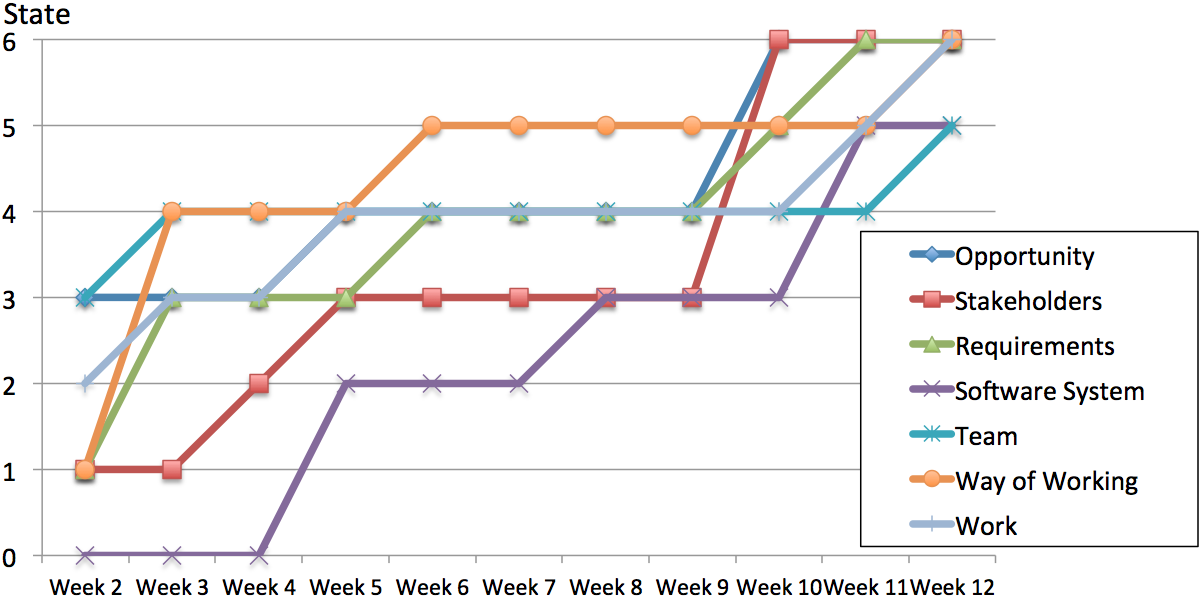
\includegraphics[width=3.30in]{project_steering_images/AlphaProgressionColocated3.png}
\caption{Alpha progression for team Co-located-3}
\label{AlphaProgressionColocated3}
\end{figure}


By analyzing the work items generated by the team during the weekly SEMAT sessions, we find that the initial progression in Figure \ref{AlphaProgressionColocated3} is driven by those work items. Indeed these work items significantly contribute to bringing the project to a higher state. However, the final progression is done independently of Essence as the approach generates few work items at the end of the project. Most teams experienced this phenomenon, as illustrated in Figure \ref{NewWorkItemsGenerated} showing a consistent drop of work items over time.

\begin{figure}[t]
\centering
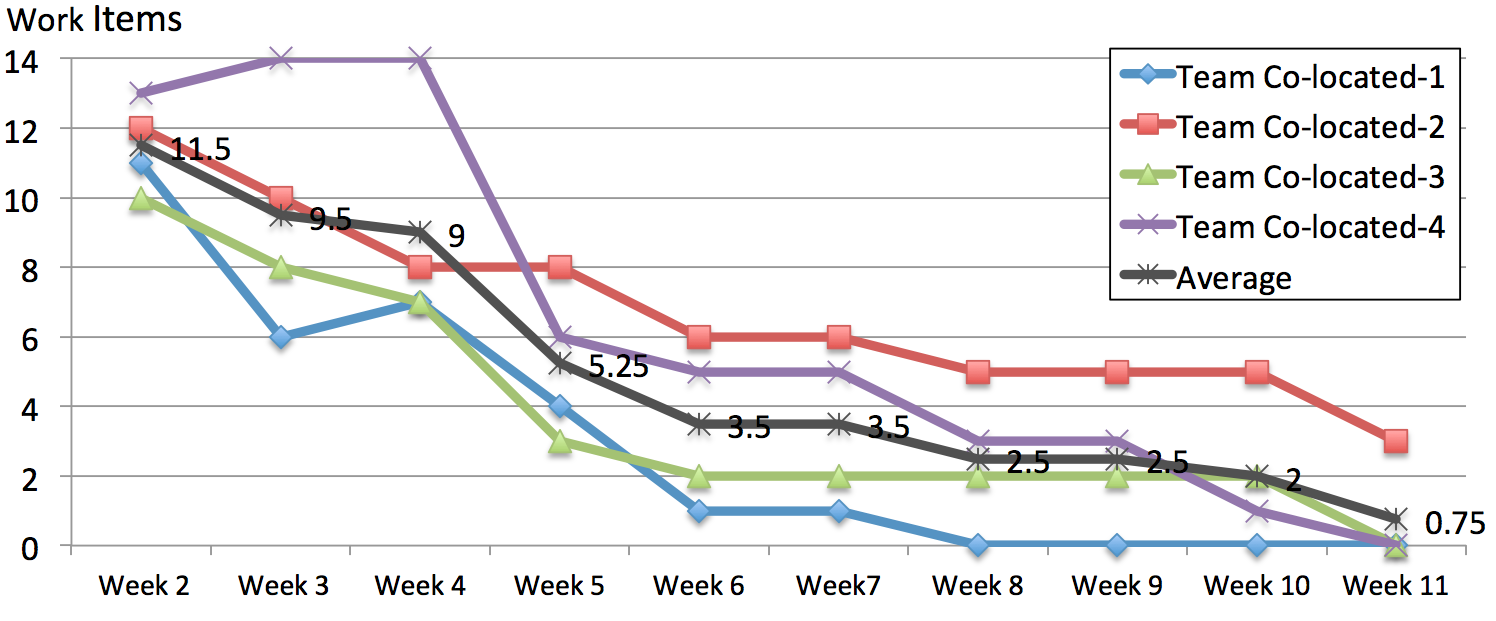
\includegraphics[width=3.30in]{project_steering_images/NewWorkItemsGenerated.png}
\caption{New work items generated per week}
\label{NewWorkItemsGenerated}
\end{figure}

Despite the value decrease, the students' perception of the approach remains positive by the end of the project according to the survey responses. Indeed a majority of students answered without qualification that they found Essence worth their time and will use the approach on their next project. A majority of students also mentioned reflection or retrospective as a strength of the approach. One student mentioned: \participantQuote{Even though we are not generating new tasks, the [SEMAT] meetings remain useful as they give us the opportunity to reflect upon our project.} Similarly, team Distributed-1 noted in its reflection report: \participantQuote{The team was pleased to see that Essence covered `The Way of Working' as well as ‘The Team'. These two topics generated useful team introspection at the beginning of the practicum and were nice reminders that the team does constant checkups for the overall condition of the members and the project.}

In conclusion, the SEMAT Essence's monitoring and steering approach provided by the kernel alphas and their states is most effective at the beginning of the project. The effectiveness decreases over time. Indeed, the approach gradually loses its ability to enable the team to steer the project by generating new work items leading to a higher project state. The reasons behind the value decrease are explored in the next research question. However, most teams continue to perceive value throughout the lifecycle out of the approach reflection mechanism.

\textbf{Research Question 4}: What are the limitations to the approach's effectiveness?

The previous section shows that the effectiveness of the approach decreases over time. This phenomenon could be explained by a number of factors. One factor relates to the fact that the need for the approach varies throughout the project lifecycle. For instance, as the project team matures and becomes a high-performing team producing high quality outcome, it becomes a self-steering team requiring less support from the approach. Similarly, once most project risks have been mitigated, the team requires less risk management support. Therefore, unless there is a disruptive event reverting the project to a lower state, the value decrease is to be expected.

In addition, some kernel characteristics influence the value decrease. Most Essence alphas have more states supporting the progression through the initial project phase compared to later phases. Figure \ref{NumberOfAlphaStatesPerRUPPhase} illustrates this phenomenon using the RUP \cite{KrollRUP} phases (Inception, Elaboration, Construction, and Transition) as an example. The chart shows that for most alphas, the number of states per phase is higher in Inception compared to the other phases. For five out of seven alphas, there is only one state in Construction. Most project teams spend the majority of their time in Construction. As a result, for these alphas the teams end-up remaining in the same state during their entire Construction phase. This lack of alpha states covering the Construction phase might be due to the fact that most of the technical work done in Construction is practice-specific, and therefore not supported by the universal kernel. Further investigations are necessary to identify potential ways to extend the kernel so it better supports the work done during Construction.

\begin{figure}[t]
\centering
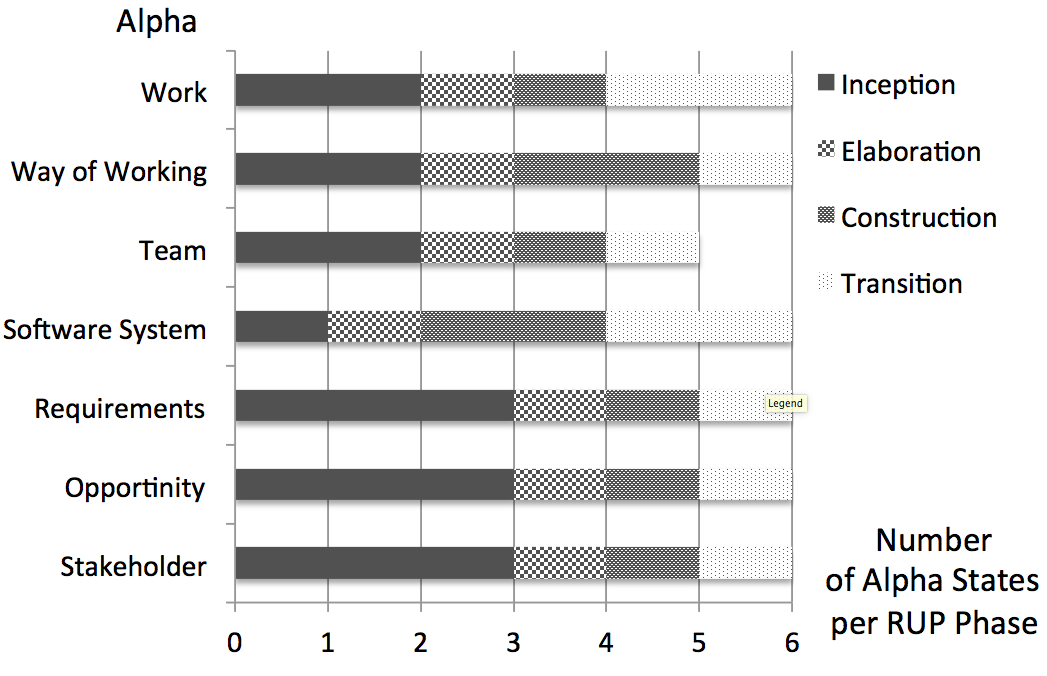
\includegraphics[width=3.30in]{project_steering_images/NumberOfAlphaStatesPerRUPPhase.png}
\caption{Number of alpha states per RUP phase}
\label{NumberOfAlphaStatesPerRUPPhase}
\end{figure}

By definition, the Essence kernel is geared towards steering a project or release throughout its entire lifecycle in a fairly linear fashion dictated by the alpha state progression. By repeating through the Essence monitoring and steering loop (see Figure \ref{EssenceMonitoringLoop}), the team steers the project or release through the sequence of states for each alpha. This process is designed to support the work done at the release level and not to support the work done at the iteration level because of the following reasons:

\begin{itemize}
    \item The kernel is lifecycle-independent and therefore does not provide specific support for iterative development.
    
    \item The kernel alpha states and their checklist items are specified at the project or release level, not at the iteration level.
\end{itemize}

Consequently, we were unable to effectively leverage the approach to help steer projects during Construction on iterative projects. The teams received some guidance on iterative development from whatever method they adopted, like Scrum and XP that are optimized for iterative development.

In conclusion, the observed value decrease could be explained by three factors. The first factor is a decrease in the need for the approach as the team matures and becomes self-steering. The second factor is a front-end focus of the alphas, making the approach most effective during project initiation. The third factor relates to the definition of the kernel alpha checklists, which are specified at the project or release level, not at the iteration level. This explains the value decrease during construction on iterative projects.

As a result, the monitoring and steering mechanisms are most effective during project initiation and for monitoring and steering the work done at the project or release level. This type of work could be qualified as \quotes{universal} as it is generally common across projects. This confirms that the kernel provides effective support for universal work. Support for non-universal technical work has to come from additional practices added on top of the kernel, or by extending or altering the kernel definition.

Finally, a limitation pointed out by about 40\% of the students in the survey, is related to some ambiguity in the alpha checklists definition. For instance, one student mentioned: \participantQuote{The checklist within an alpha can have cryptic language. Sometime, the points are ambiguous.} Here are some examples of typical student reactions:

\textbf{Checklist Item}: Enough of the requirements are addressed \ldots 

\textbf{Student}: \participantQuote{What do they mean by `enough'?}

\textbf{Checklist Item}: Constraints are identified and considered. 

\textbf{Student}: \participantQuote{What kind of constraints are they talking about?}

\textbf{Checklist item}: Critical interfaces have been demonstrated. 

\textbf{Student}: \participantQuote{What do they mean by `demonstrated'?}

\textbf{Checklist Item}: The key practices and tools that form the foundation of the way-of-working are selected.

\textbf{Student}: \participantQuote{Which tools form the foundation of the way-of-working?}

Thus, a limitation to the approach effectiveness comes from some ambiguities in the alpha checklist definitions, leading to situations where the team discusses the meaning of a checklist item instead of having a conversation about the project. At times, this disrupts the flow of otherwise valuable team discussions.

\section{FROM THE EDUCATOR'S PERSPECTIVE}
This section shares some of our findings related to introducing Essence to a project team having no prior experience with the approach, together with a few words of caution related to the use or misuse of Essence for evaluation purposes.

\subsection{Incremental versus Workshop Introduction Approaches}

Our experience with both the incremental and workshop approaches to introducing Essence indicates that both have value and that adoption resistance drives which approach is best for the situation.

\subsubsection{Incremental}
The incremental introduction approach brings immediate value to the teams, as noted by team Distributed-2 in its reflection report: \participantQuote{The team found Essence valuable right from the start. [...] it helped manage the direction and organization of the team by examining overlooked aspects of the project.} For instance, during the first session, this team identified the work items \quotes{Understand the risks and constraints} and \quotes{Identify all stakeholders} based on its discussion around the \textbf{Opportunity} alpha and \textbf{Stakeholder} alpha respectively. Some previous practicum teams overlooked these kinds of discussions and work items. However, this approach delays many important conversations until all the alphas are introduced.

This approach has minimum perceived overhead. In our case, introducing Essence incrementally required only a weekly session of 30 minutes, during a five weeks period.

When adoption resistance might be an issue, we recommend introducing the approach incrementally through a series of regular (e.g. weekly) and short (e.g. 30 minutes) sessions. We also recommend having one dedicated faculty or coach per team.

\subsubsection{Workshop}
The workshop introduction approach introduces all the alphas at once, hence enabling the team to look at its project holistically while having conversations covering the various project's dimensions as early as possible.

This approach requires that each team invest in one upfront workshop during which the team starts applying Essence directly to its current project. During our 90 minutes introduction workshop, 10 minutes were needed to set the context and motivate the exercise. The remaining 80 minutes was enough time for most teams to have a substantial conversation about their perception of the project's current state and to generate work items to make forward progress. On average, 10 minutes were necessary for a team to cover one alpha, and most teams were able to cover the seven alphas during the workshop. However, our largest team of five members took an average of 20 minutes per alpha and hence had to complete the exercise during a follow-up session. The size of the team as well as internal disagreements generated some longer conversations.

We recommend adjusting the workshop duration based on the team size and any other known parameters that might influence the length of the conversations, like team dynamic or project uncertainty. We also recommend having one dedicated faculty or coach per team.

Table \ref{ComparingWorkshopAppoaches} summarizes and compares the incremental and workshop introduction approaches. We recommend the workshop approach when introducing Essence, unless faced with initial adoption resistance that may require a slower incremental approach.

\begin{table}[]
\centering
\renewcommand{\arraystretch}{1.4}
\caption{Comparison of introduction approaches}
\label{ComparingWorkshopAppoaches}
\begin{tabular}{|p{0.6in}|p{1.1in}|p{1.1in}|}
\hline
Approach      & Incremental                                                                 & Workshop  \\
\hline
Description   & Essence alphas are introduced incrementally over a number of short sessions & Essence alphas are introduced all at once during a single session \\
\hline
Benefits      & Brings immediate value with minimum overhead                                & Brings immediate and optimum value (all alphas are covered)       \\
\hline
Drawbacks     & Full benefit is delayed until complete introduction of alphas               & Requires initial overhead                                         \\
\hline
When to Apply & In case of adoption resistance                                              & Always, except in case of adoption resistance  \\                  
\hline
\end{tabular}
\end{table}

Given our recommendation of one faculty per team, in the future, we plan on introducing Essence and conducting a full assessment during a 90-minute team meeting. In a course with five teams, scheduling five separate team meetings is easier than trying to do five simultaneous team meetings with five instructors.

Following the introduction of Essence, we recommend that each project team continue to meet on a regular (e.g. weekly) basis for a short (e.g. 30 minutes) session throughout the initial project phase. Once a team reaches \quotes{construction} and becomes a high-performing team producing high quality outcome, the frequency of the sessions could decrease because the team needs less support from the approach.

\subsection{Alpha Introduction Order}
Participants can be overwhelmed when shown all the states for all the alphas at once. Introducing the alphas one at a time solves this problem, whether this is done incrementally over a series of meetings or during a single session or workshop.

We recommend introducing the \textbf{Stakeholder} and \textbf{Opportunity} alphas (aka the customer dimension) first, since it generally makes sense to have a discussion around this dimension before drilling down into the details of the solution and endeavor. We introduce \textbf{Stakeholder} prior to \textbf{Opportunity} since many participants find it easier to relate to the \textbf{Stakeholder} alpha than the abstract \textbf{Opportunity} alpha. The other alphas could be introduced as needed based on pain points. When in doubt about which alpha to introduce next, one alpha could be selected randomly. Indeed, the value is in having a holistic view of the project, therefore looking at any dimension has potential benefits.

\subsection{A Word of Caution}
As noted by William Cameron \cite{CameronSociologicalThinking}, \quotes{not everything that can be counted counts, and not everything that counts can be counted.} This is especially true when it comes to individual and team performance evaluation, where using metrics could be dangerous. Inappropriate metrics could be used (like measuring a developer performance based on the number of lines of code produced), metrics could be gamed, and metrics do not give the full picture.

As an example, Figure \ref{AvoidThisKindOfComparison} shows the final state of our distributed teams at the end of their project. From the chart, one might infer that Team Distributed-3 outperformed Team Distributed-1, which in turn outperformed Team Distributed-2 that lagged behind. In fact, despite having the highest project state, Team Distributed-3's work was slightly disappointing according to both the clients and faculty. The team ended-up with a lower grade compared to the other teams. This was due to quality issues during various product demonstrations and a lack of architecture documentation that surfaced during the team final presentation. This makes the team self-assessment of the \textbf{Software System} alpha and therefore of its overall project state questionable. Team Distributed-2 lagged only behind because the initial solution proposed by the client turned out to be infeasible, and the team did an excellent job redirecting the project into a constructive direction and hence earned an excellent grade. The routinely low \textbf{Software System} alpha state served as a red flag for risk management purposes, not evaluation purposes.

\begin{figure}[t]
\centering
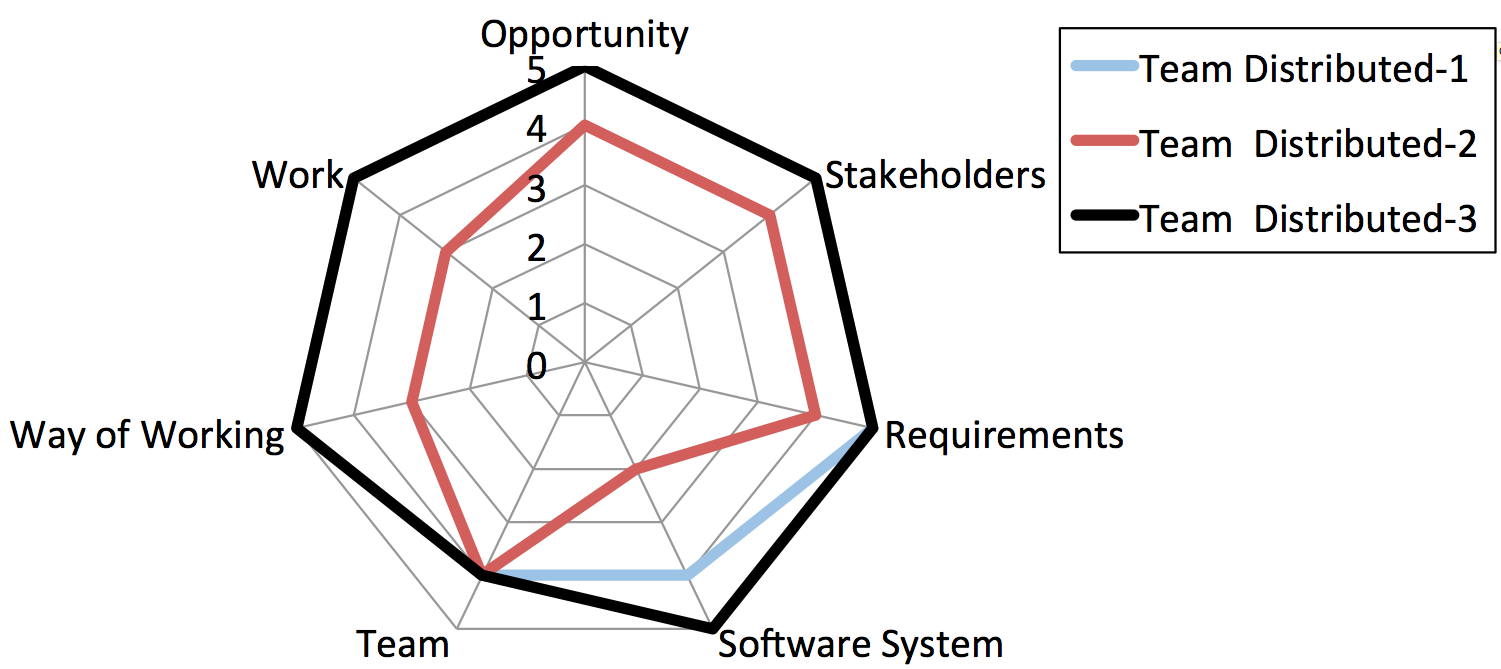
\includegraphics[width=3.30in]{project_steering_images/AvoidThisKindOfComparison.png}
\caption{Final project state of the distributed teams: Avoid this kind of comparison}
\label{AvoidThisKindOfComparison}
\end{figure}


In conclusion, we recommend leveraging the approach to identify projects at risk rather than for performance evaluation purposes. Some teams might be only ahead because they are overly optimistic about their project state, while others might be behind because of circumstances beyond their control.

\section{CONCLUSION}
This paper presents the results of a field study aiming at understanding the value project teams receive from following the SEMAT Essence's monitoring and steering approach provided by the Essence kernel alphas and their states. The study involved seven teams of master students with no prior knowledge of Essence.

The study validated our research hypothesis by showing that the approach provides student teams with a simple, lightweight, non-prescriptive and method-agnostic way to examine their projects holistically, structure team reflections, manage risks, monitor progress and steer their projects. Compared to the ten previous years, the faculty in charge of the practicum course noted that there was \participantQuote{much better early project organization with a lot less floundering.} Indeed, the approach enables students to learn to steer projects effectively by addressing the various dimensions of software engineering.

The study also highlighted that the monitoring and steering mechanisms are most effective during project initiation and for monitoring and steering the work done at the project or release level. This type of work could be qualified as \quotes{universal} as it is generally common across projects. This confirms that the kernel provides an effective support for universal work. Support for non-universal technical work should come from additional practices added on top of the kernel, or by extending or altering the kernel definition.

The results of this paper are limited to evaluating the effectiveness of the Essence approach when a facilitator is involved. Even though faculty involvement was kept at a minimum to limit influencing the students, a faculty served as facilitator during the SEMAT meetings throughout the practicum projects. More research is necessary to assess the effectiveness of the approach without facilitators.

The project context was fairly similar for all teams, except for their geographic distribution and average work experience. While the study has not revealed any influences of these contextual factors on the approach's effectiveness, additional data is required to confirm or refute any impact. The Essence steering and monitoring approach appears equally applicable to both co-located and geographically distributed teams.

We are currently working with another set of practicum teams at Carnegie Mellon University in Silicon Valley to gather more data necessary to evaluate the SEMAT Essence's monitoring and steering approach, with a focus on both effectiveness of the approach and accuracy of the model.

\section{ACKNOWLEDGMENTS}
We would like to acknowledge the contributions of all the reviewers, and thank them for their insightful comments on early drafts of this paper. A special thanks to Hakan Erdogmus and Maria Nelson for their thorough reviews and invaluable suggestions, and to Ed Katz for recommending that we conduct our field study in the context of his practicum course and for his support throughout the study. Finally, we would like to warmly thank the students who participated in the study, for their openness and insights.

\section{APPENDIX}
Figure \ref{FieldStudyRowData} below provides the reader with the field study row data on alpha state progression. Each number in bold (from 1 to 6) represents an alpha state. Each number in italic (from 2 to 15) represents the week during which the team reaches the state. For instance, team Distributed-1 reaches the \textbf{Stakeholder} state 1 at week 2. Two or more italic numbers in one cell reflects a state backtracking. For instance, team Co-located 2 reaches the \textbf{Team} state 3 at week 2. The team then progresses to a higher state, but backtracks to state 3 at week 10.

\begin{figure*}[h]
\centering
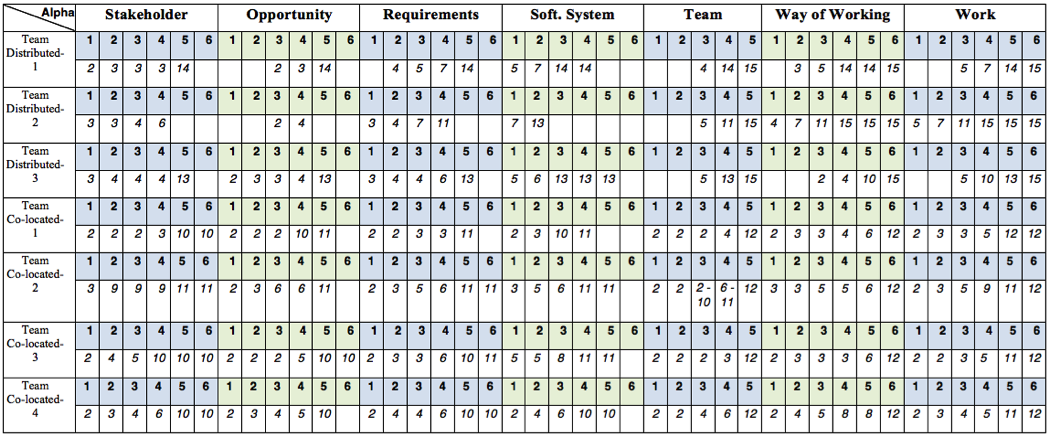
\includegraphics[width=6.80in]{project_steering_images/FieldStudyRowData.png}
\caption{Field study row data on alpha state progression}
\label{FieldStudyRowData}
\end{figure*}


% \begin{table*}[]
% \centering
% \renewcommand{\arraystretch}{1.3}
% \caption{Field study row data on alpha state progression}
% \label{FieldStudyRowDatal}
% \begin{tabular}{|l|l|l|l|l|l|l|l|l|l|l|l|l|l|l|l|l|l|l|}
% \hline
%                   & \multicolumn{6}{l|}{Stakeholders} & \multicolumn{6}{l|}{Opportunity} & \multicolumn{6}{l|}{Requirements} \\ \hline
%                   & 1   & 2   & 3   & 4   & 5   & 6   & 1   & 2   & 3  & 4   & 5   & 6   & 1   & 2   & 3   & 4   & 5   & 6   \\ \hline
% Team Distributed-1 & 2   & 3   & 3   & 3   & 14  &     &     &     & 2  & 3   & 14  &     &     & 4   & 5   & 7   & 14  &     \\ \hline
% Team Distributed-2 & 3   & 3   & 4   & 6   &     &     &     &     & 2  & 4   &     &     & 3   & 4   & 7   & 11  &     &     \\ \hline
% Team Distributed-3 & 3   & 4   & 4   & 4   & 13  &     & 2   & 3   & 3  & 4   & 13  &     & 3   & 4   & 4   & 6   & 13  &     \\ \hline
% Team Co-located-1  & 2   & 2   & 2   & 3   & 10  & 10  & 2   & 2   & 2  & 10  & 11  &     & 2   & 2   & 3   & 3   & 11  &     \\ \hline
% Team Co-located-2  & 3   & 9   & 9   & 9   & 10  & 11  & 2   & 3   & 6  & 6   & 11  &     & 2   & 3   & 5   & 6   & 11  & 11  \\ \hline
% Team Co-located-3  & 2   & 4   & 5   & 10  & 10  & 10  & 2   & 2   & 2  & 5   & 10  & 10  & 2   & 3   & 3   & 6   & 10  & 11  \\ \hline
% Team Co-located-4  & 2   & 3   & 4   & 6   & 10  & 10  & 2   & 3   & 4  & 5   & 10  &     & 2   & 4   & 4   & 6   & 10  & 10  \\ \hline
% \end{tabular}
% \end{table*}


% \begin{table*}[]
% \centering
% \caption{My caption}
% \label{my-label}
% \begin{tabular}{|l|l|l|l|l|l|l|l|l|l|l|l|l|l|l|l|l|l|l|l|l|l|l|l|l|l|l|l|l|l|l|l|l|l|l|l|l|l|l|l|l|l|}
% \hline
%                   & \multicolumn{6}{l|}{Stakeholders} & \multicolumn{6}{l|}{Opportunity} & \multicolumn{6}{l|}{Requirements} & \multicolumn{6}{l|}{Software System} & \multicolumn{5}{l|}{Team} & \multicolumn{6}{l|}{Way of Working} & \multicolumn{6}{l|}{Work} \\ \hline
%                   & 1   & 2   & 3   & 4   & 5   & 6   & 1   & 2   & 3  & 4   & 5   & 6   & 1   & 2   & 3   & 4   & 5   & 6   & 1    & 2   & 3    & 4    & 5   & 6   & 1   & 2  & 3  & 4   & 5   & 1   & 2   & 3   & 4    & 5    & 6   & 1  & 2  & 3 & 4 & 5  & 6  \\ \hline
% Team Distributed-1 & 2   & 3   & 3   & 3   & 14  &     &     &     & 2  & 3   & 14  &     &     & 4   & 5   & 7   & 14  &     & 5    & 7   & 14   & 14   &     &     &     &    & 4  & 14  & 15  &     & 3   & 5   & 14   & 14   & 15  &    &    & 5 & 7 & 14 & 15 \\ \hline
% Team Distributed-2 & 3   & 3   & 4   & 6   &     &     &     &     & 2  & 4   &     &     & 3   & 4   & 7   & 11  &     &     &      &     &      &      &     &     &     &    &    &     &     &     &     &     &      &      &     &    &    &   &   &    &    \\ \hline
% Team Distributed-3 & 3   & 4   & 4   & 4   & 13  &     & 2   & 3   & 3  & 4   & 13  &     & 3   & 4   & 4   & 6   & 13  &     &      &     &      &      &     &     &     &    &    &     &     &     &     &     &      &      &     &    &    &   &   &    &    \\ \hline
% Team Co-located-1  & 2   & 2   & 2   & 3   & 10  & 10  & 2   & 2   & 2  & 10  & 11  &     & 2   & 2   & 3   & 3   & 11  &     &      &     &      &      &     &     &     &    &    &     &     &     &     &     &      &      &     &    &    &   &   &    &    \\ \hline
% Team Co-located-2  & 3   & 9   & 9   & 9   & 10  & 11  & 2   & 3   & 6  & 6   & 11  &     & 2   & 3   & 5   & 6   & 11  & 11  &      &     &      &      &     &     &     &    &    &     &     &     &     &     &      &      &     &    &    &   &   &    &    \\ \hline
% Team Co-located-3  & 2   & 4   & 5   & 10  & 10  & 10  & 2   & 2   & 2  & 5   & 10  & 10  & 2   & 3   & 3   & 6   & 10  & 11  &      &     &      &      &     &     &     &    &    &     &     &     &     &     &      &      &     &    &    &   &   &    &    \\ \hline
% Team Co-located-4  & 2   & 3   & 4   & 6   & 10  & 10  & 2   & 3   & 4  & 5   & 10  &     & 2   & 4   & 4   & 6   & 10  & 10  &      &     &      &      &     &     &     &    &    &     &     &     &     &     &      &      &     &    &    &   &   &    &    \\ \hline
% \end{tabular}
% \end{table*}

% \chapter{Essence Green Lighting}
\section{Abstract}

Many software engineering curriculum conclude with a
practicum or capstone project course. For courses involving external
clients, the course owner typically follows a Request for Proposal
process to vet (or green-light) qualified clients and projects.

Even though green-lighting projects does not guarantee project success, 
the goal is to reduce risks by systematically examining each proposal to identify
potential problems that the instructor could solve, mitigate against, 
or simply decide not to deal with by rejecting the proposal.

We propose and evaluate a Green-Lighting Approach based on the
SEMAT (Software Engineering Method and Theory) Essence framework. 
Our objective is to identify if such a framework could improve the Request for Proposal process 
at Carnegie Mellon University in Silicon Valley and other universities.

We conducted a case study by observing and interviewing the
course owner, examining a group of proposals, and identifying issues
with the current proposal process and practicum projects.
We proposed a green-lighting project state that, based upon Essence Alphas,
describes the minimal and ideal states that a project proposal should achieve to be accepted. 

The Green-Lighting Approach generated conversations among the faculty 
that clarified the guidelines for accepting and prioritizing proposals and identified deficiencies in our Request for Proposal. Additional work is required to refine the proposed Green-Lighting Approach based on current findings and further validate the approach.
  
Using Essence for green-lighting practicum projects in academia presents some limitations. 
The framework does not explicitly factor in business forces that affect proposal selection,
might be overly complex for the task, and might require modification with partial Alpha states. 
However, Essence provides a systematic approach for evaluating proposals based on various project dimensions. 
This approach could be used as an inspiration for deriving simpler custom green-lighting checklists. 

\section{Introduction}
\label{Introduction}

Many software engineering (SE) curricula finish with a practicum course
or capstone project \cite{GSWE}. At Carnegie Mellon
University in Silicon Valley, the curriculum culminates with a practicum
course in order for the students to demonstrate mastery of the
curriculum and to learn client management skills
\cite{Katz}. The practicum allows students to reinforce
their learning of core software engineering knowledge by applying this
knowledge to a different problem or domain. The practicum serves as
confirmation that the student has mastered the material. Earlier in the
curriculum, faculty manage the students project courses by playing the
customer or management role. The practicum provides an opportunity for
the students to work with a real client and practice client management
skills. Students actively manage the client engagement while faculty
observe and coach students without interfering unless necessary. The
students perform as a consulting team delivering a product that addresses the client's opportunity.

The university wants to increase its impact through the practicum
projects. The practicum course owner needs to find projects that
balance these goals:

\begin{itemize}
\itemsep1pt\parskip0pt\parsep0pt
\item
  maximize the students' learning experience, 
\item
  achieve a business goal or positively impact society, and
\item
  increase collaborations between university and industry. 
\end{itemize}

In order to accomplish the practicum goals, the faculty want to offer
a portfolio of projects including

\begin{itemize}
\itemsep1pt\parskip0pt\parsep0pt
\item
  a mix of project domains,
\item
  a mix of startups and established companies, and 
\item
  a mix of exploratory research and well defined
  endeavors.
\end{itemize}

Since we have a limited number of students and thus student teams, the
course owner needs to be selective about proposals with respect to these
goals. The course owner needs a systematic, non biased technique to
filter proposals.

\section{Related Work}
\label{Related Work}
Many software engineering professors have described their approach to providing a practical hands on experience. Most of the literature describes in detail how to run a team-based project course yet there is little discussion about the client selection process. 

In 1991, Shaw and Tomayko \cite{shaw1991models} examined hundreds of undergraduate software engineering courses and interviewed scores of instructors. In their technical report, they identify two major decisions that the instructor must make: 1) deciding the mixture of lecture and project components and 2) deciding the balance technical and managerial skills taught in the course. 

They describe several course models used in academia including the ``small group project'' model, ``large project team,'' model, and  ``the project only'' model. The ``small group project'' and  ``large project team'' models infuse lectures with a course long project. The ``project only'' model is typically a capstone course that focuses on the project experience.

Shaw and Tomayko discusses the importance of finding an interesting project that will motivate the students for the duration of the course, but provides no model for client selection.

In 2001, Cal Poly \cite {Turner2001} introduced a year long capstone project course. For the first two years, they relied on one industrial partner for the entire course, but due to coordination difficulties replaced the external project with a university project. No guidance is provided for project selection.

In 2002, Chamillard and Braun \cite{Chamillard2002} reflect on an undergraduate course at the U.S. Air Force Academy. They focus on tradeoffs such as the amount of guidance, documentation formats versus documentation examples, and focusing software development process versus product. They do not discuss their client selection process.

In 2002, Umphress, Hendrix, and Cross \cite{Umphress2002} reflect on their 18 years of experience and describe the transformation of processes from ad hoc, to MIL-STD-498 to IEEE 1074 to the Team Software Process to Extreme Programming. No information is provided about client selection.

In 2006, Coppit \cite{coppit2006} describes his strategies for overcoming the difficulties in running a large project team course including how to assess student performance. In his section on project selection, he briefly recommends that the amount of work should be commiserate with the length of the course, the scope needs to be flexible to allow cutting of features at the course's end, and have significant parallelizable work. 

In 2010, Ziv and Patil \cite {ziv2010capstone} discuss the experience of transitioning a capstone from one quarter to a three quarter course. The course follows a ``small group project'' model with external clients. The instructors typically have enough projects for all the enrolled students. Regarding selection criteria, the instructors take most projects within reasonable size, scope, goals and objectives, and reject only when the instructors notice a complete misunderstanding of the nature and purpose of a college-level undergraduate-level student project. 

Overall, criteria for client selection in the context of academic projects is only briefly discussed in the literature. 

\section{Background}
\label{Background}
For the past four semesters, we applied the Project Monitoring and
Steering Approach ~of the Essence framework
\cite{EssenceBook} in weekly Essence Reflection
Meetings \cite{EASE2014}. The approach provides student
teams with a simple, lightweight, non- prescriptive and method-agnostic
way to examine their projects holistically, structure team reflections,
manage risks, monitor progress and steer their projects
\cite{ICSE2014}.

During the research of applying the Project Monitoring and Steering
Approach, we observed practicum issues regarding stakeholder
representation, understanding the value of the opportunity, and undefined project scope and success criteria. Some aspects of these issues might be attributed to some extent to the way in which the practicum proposals are initiated and accepted. For example, one client believed that she could represent several different user personas and was unwilling for student teams to interview potential users. Our motivation is to examine our Request for Proposal process could help address these issues.

We proposed and applied a Green-Lighting Approach based on the Essence framework \cite{EssenceBook}. Our objective is to identify if such a framework could potentially improve the Request for Proposal process at Carnegie Mellon University in Silicon Valley and other universities.

The Green-lighting Approach
uses the Essence Alphas to describe how ready the project should be in
each Alpha, which we'll call ``green-lighting project state'' in this
paper. The green-lighting project state serves as a gating function,
filtering out unready projects.

In this paper, we will introduce the Green-lighting Approach which
provides a gating function for proposals. Section
\ref{Field Study Description} describes the field study
including the research goal, the current Request for Proposal, the
proposed change, and the study protocol. Section
\ref{Results} examines seven research questions
supporting the research goal. Section \ref{Conclusion}
summarizes that the findings and discusses future work.


\section{Green-lightning Approach of the Essence framework}
\label{Green-lightning Approach of the Essence framework}

In 2012, the SEMAT community released the Essence kernel
\cite{OMGStandard}. The Essence kernel describes a
software project through different dimensions called Alphas. For
example, the \textbf{Stakeholder} Alpha advances through the states
\textit{Recognized}, \textit{Represented}, \textit{Involved}, 
\textit{In Agreement}, \textit{Satisfied for Deployment}, and \textit{Satisfied in Use}. Each state has a set of checklist items. For example, \textit{Recognized} contains these three checklist items:

\begin{itemize}
\itemsep1pt\parskip0pt\parsep0pt
\item
  Possible stakeholders groups are identified
\item
  Team agrees on relevant stakeholder groups to be represented
\item
  Responsibilities of stakeholder representatives are defined
\end{itemize}

A project achieves a state when the team can check all the checklist
items for a state. This means that Essence represents projects through a
collection of linear state machines where the states are partially
ordered.

We defined the Green-lighting Approach based upon an example of using
the Essence framework from the Essence Book. Section 12: ``Running a
software endeavor: From idea to Product''
\cite{EssenceBook} describes how to use the Essence
Kernel Alpha States to define a staging process for a hypothetical
project. The example divides the project into four stages ``Getting
Ready to Start,'' ``Starting Up,'' ``Running Development,'' and
``Done.'' As the project progresses through these stages, the Alpha
states progress. In an organization managing many projects, one could
expect the projects to achieve certain states before making it into the
next stage. We define the Green-Lighting Approach to evaluate the
transitions between multiple stages.

The Green-Lighting Approach has three steps:

\begin{itemize}
\itemsep1pt\parskip0pt\parsep0pt
\item
  Evaluate each proposal and determine its state in each Alpha. For
  example, considering the  \textbf{Stakeholders} Alpha, a proposal that meets the three checklist items tor \textit{Recognized}
  and the four checklist items for \textit{Represented} would be marked as \textit{Represented} as seen in Figure
  \ref{EssenceAlpha}. This is repeated for each Alpha.
  This data can be represented as a hash where the keys are the Alphas
  and the values are the Alpha states, such as: \{stakeholders:
  ``represented'', opportunity: ``identified'', requirements:
  ``conceived'', software system: ``architecture selected''\}. The check marks in Figure
  \ref{EssenceAlpha} indicate the proposal's project
  state.
\item
  Determine the ``green-lighting project state,'' which is the minimal
  acceptable state for each Alpha. This too can be represented as a
  hash. In our example, the green-lighting project state could be:
  \{stakeholders: ``recognized'', opportunity: ``solution needed'',
  requirements: ``conceived'', software system: ``none''\}. The circled
  states in Figure \ref{EssenceAlpha} represent the
  green-lighting project state.
\item
  Applying the green-lighting project state to a proposal determines
  the project's readiness. A project is ready if the proposal has a
  larger or equal state for each Alpha in the green-lighting project
  state. Using the hash example, we compare each key of the hash and
  make sure the proposal is ``larger or equal'' to each corresponding
  key in the green-lighting project state. In the given example, the
  proposal is ready in each Alpha except Opportunity. In this regard, the approval process
  is a function with two inputs and one boolean output. F(Hash proposal,
  Hash greenlight\_project\_state) =\textgreater Boolean
  accept\_propopsal
\end{itemize}

% \begin{figure}[h]
% \includegraphics[scale=0.25]{EssenceAlpha.jpg}
% \caption{Essence alphas checked for a proposal and shaded for
% green-lighting project state}\label{EssenceAlpha}
% \end{figure}


\begin{figure}[!t]
\centering
\includegraphics[width=3.45in]{essence_green_lighting_images/EssenceAlpha.png}
\caption{Essence Alphas checked for a proposal and circled for
green-lighting project state}
\label{EssenceAlpha}
\end{figure}

In examining the seven Essence Alphas, only four Alphas,
\textbf{Stakeholders}, \textbf{Opportunity}, \textbf{Requirements}, and \textbf{Software System} are relevant to evaluating practicum proposals. The OMG standard defines these four Alphas as: \cite{OMGStandard}

\begin{itemize}
\itemsep1pt\parskip0pt\parsep0pt
\item
  \textbf{Stakeholders}: The people, groups, or organizations who affect or
  are affected by the software system.
\item
  \textbf{Opportunity}: The set of circumstances that makes it appropriate to
  develop or change a software system.
\item
  \textbf{Requirements}: What the software system should do to address the
  opportunity and satisfy the stakeholders
\item
  \textbf{Software System}: A system made up of software, hardware, and data
  that provides its primary value by the execution of the software.
\end{itemize}

The other three Essence Alphas (\textbf{Team, Way of Working} and \textbf{Work}) only make sense once a student team is
assigned to the project. Indeed, the \textbf{Team} has not been assembled yet,
hence it does not have a \textbf{Way of Working} and has not performed any
\textbf{Work}. By course design, the client does not determine the team's
\textbf{Way of Working}.


\section{Field Study Description}
\label{Field Study Description}

Following recommendations for reporting research done in the empirical
software engineering community
\cite{GQM, Shaw}, we formed our
research goal using Goal/Question/Metric:
\cite{GQM}

\begin{table}[h]
\renewcommand{\arraystretch}{1.3}
\centering
\begin{tabular}{|p{1.00in}|p{2.10in}|}
\hline
Analyze & SEMAT Essence’s Green-lighting Approach provided by the kernel Alphas and their states \\ \hline
for the purpose of & evaluation \\ \hline
with respect to its & effectiveness \\ \hline
from the point of view of the & educator and researcher \\ \hline
in the context of  & the software engineering practicum graduate course at Carnegie Mellon University. \\
\hline
\end{tabular}
\end{table}


This paper decomposes this goal into the following questions:


\begin{itemize}
\itemsep1pt\parskip0pt\parsep0pt
\item
  \textbf{Research Question 1}: What is the initial state of most projects
  based on the current proposals?
\item
  \textbf{Research Question 2}: What are some problems with the practicum that could potentially be mitigated to some extent prior to the start of the project?
\item
  \textbf{Research Question 3}: From the faculty perspective, what should be
  the minimum or ideal initial state of a project?
\item
  \textbf{Research Question 4}: How do the proposals compare against the
  proposed minimum and ideal green-lighting project states?
\item
  \textbf{Research Question 5}: Do we need to improve the Request for
  Proposal?
% \item
%   \textbf{Research Question 6}: What is the effect of using the Essence
%   Green-lighting Approach on the time it takes to accept or reject a
%   project?
\item
  \textbf{Research Question 6}: What are limits to the approach and
  limitations to its effectiveness?
\end{itemize}


\subsection{Current Practicum Request for Proposal}
\label{ProposalQuestions}

Prior to the start of the course, the course owner solicits project
proposals from industry and colleagues. The current practicum Request
for Proposal asks sponsors to create and provide a document including
the following information:

\begin{itemize}
\itemsep1pt\parskip0pt\parsep0pt
\item
  {Name of the project}
\item
  {Summary of the project}
\item
  {Overview of the sponsoring organization}
\item
  {Background and problem context }
\item
  {Relevance and Opportunity: why is it important and who benefits}
\item
  {Proposed scope of work}
\item
  {Major project goals and objectives }
\item
  {Technologies and skill sets requirements }
\item
  {Expected team size }
\item
  {Currently known obstacles}
\item
  {Nature of working relationship with sponsoring organization}
\item
  {Expected use of deliverables at project completion}
\item
  {Preliminary project roadmap}
\item
  {Criteria for measures of success}
\item
  {Any IP, NDA, or citizenship constraints}
\end{itemize}

The course owner wants any submitted proposal to clearly communicate
the project's big picture, the client's needs, and a general project
roadmap. At the due date, the course owner reviews the submitted
proposals to verify their completeness. The course owner verifies that
the project is an appropriate educational experience, and relies on the
students to filter the projects. The course owner encourages
students to contact the client for clarification, if necessary.

Given the number of students enrolled in the course, the course owner
determines the expected number of teams for the course. In years when
there are significantly more project proposals than expected number of
teams, the students use dot voting to cull the list down to a manageable
number. For example, for 32 students, there might be 6 to 8 teams. If
there are 16 acceptable proposals, the course owner reduces it to 12
practicum proposals by the students dot voting their favorite projects.

Once there is a ``shortlist'' of proposals, the course owner invites
all the clients and students to a practicum fair. The course owner asks
the students to be familiar with all of the practicum proposals. The
purpose is to provide a forum for the students to ask the clients
specific questions about the project, not for the client to give a
complete presentation about the project. The clients introduce themselves
and have a summary slide or two to remind the students about their
project. 

The students then submit a ranked ordering of all the projects from
their number one pick to their least favorite, and the course owner
forms teams. The course owner tries to assign students based upon their
first or second top choice while prioritizing paying clients. However,
this is not always possible when too many students select the same
project or when only one student selects a project.

\subsection{Proposed Practicum Request for Proposal}

We consider a modification to the current practicum Request for
Proposal process by adding a filtering step after the proposal are
received but before the proposals are shown to the students. For each
proposal, we evaluate the project's state described by the proposal
against a green-lighting project state defined using SEMAT Essence Alpha
states. The course owner only offers the students proposals that have
reached or exceeded the green-lighting state. If a proposal does not
meet the minimum criteria, then either the course owner rejects the
proposal or the course owner discusses issues with the sponsor to
illicit more information.

Various elements, like the university relationship with the client, or financial considerations, are not taken into account by the SEMAT Essence Kernel, which is the first identified limitation of the framework for the purpose of green-lighting projects in academia.

\subsection{Study Protocol}

The study protocol is as follows:

\begin{enumerate}
\itemsep1pt\parskip0pt\parsep0pt
\item
  We reviewed 21 submitted practicum proposals and
  identified their initial project state (refer to \textbf{Research Question
  1} for more information). In order to remove anchoring bias, we examined
  and rated each proposal independently. Any discrepancies were
  discussed in person.
\item
  Based upon our experience of observing the practicum course in the
  context of prior investigations \cite{EASE2014, ICSE2014},
  using a brainstorming session, we identified recent issues that
  might be addressable to some extent prior to the start of the course (refer to
  \textbf{Research Question 2} for more information).
\item
  During the same brainstorming session, we recommended a minimum and
  an ideal green-lighting project state, with the purpose of addressing
  the identified issues prior to the start of the course. The minimum
  and ideal states need to be realistic and feasible with respect to the
  kinds of projects that we receive (refer to \textbf{Research Question
  3} for more information).
\item
  We compared the state of 21 submitted proposals against the proposed
  minimum and ideal green-lighting project states (refer to \textbf{Research
  Question 4} for more information). Again, in order to remove
  anchoring bias, we reviewed and rated each proposal independently. Any
  discrepancies were discussed in person.
\item
  We proposed modifications to the current questions in the Request for
  Proposal to better reveal the initial green-lighting project state. We
  evaluated the new questions with the sponsors (refer to \textbf{Research
  Question 5} for more information).
\item
  We analyzed the study results and drew conclusions on the benefits
  and drawback of the proposed approach (refer to \textbf{Research Question 6
  } for more information).
\end{enumerate}

\section{Results and Discussion}
\label{Results}

\subsection{Research Question 1: What is the initial
state of most projects based on the current proposals?}

We started the Green-lighting Approach research by assessing the
initial states of the \textbf{Stakeholders}, \textbf{Opportunity},
\textbf{Requirements} and \textbf{Software System} Alphas for 21 proposals.

For the \textbf{Stakeholder} Alpha, we observed that:
\begin{itemize}
\itemsep1pt\parskip0pt\parsep0pt
\item
  33\% did not achieve any state. These proposals did not identify
  stakeholder groups.
\item
  48\% were in the \textit{Recognized} state. These proposals identified the
  stakeholder groups, but did not appoint the representatives.
\item
  19\% were in the \textit{Represented} state. These proposals
  identified the stakeholder groups and the representatives of each
  group.
\end{itemize}

For the \textbf{Opportunity} Alpha, we observed that:
\begin{itemize}
\itemsep1pt\parskip0pt\parsep0pt
\item
  53\% were in the \textit{Identified} state. These proposals indicated the
  need for a software solution with the stakeholders wishing to make an
  investment.
\item
  33\% were in the \textit{Solution Needed} state. These proposals clearly
  articulated the problem with confirmation on the need for a solution.
\item
  14\% were in the \textit{Value Established} state. These proposals
  established the business value with a clear definition of desired
  outcomes and success criteria.
\end{itemize}

For the \textbf{Requirements} Alpha, we observed that:
\begin{itemize}
\itemsep1pt\parskip0pt\parsep0pt
\item
  5\% did not achieve any state.
\item
  71\% were in the \textit{Conceived} state. These proposals captured the 
  itemize system purpose with the user types involved.
\item
  19\% were in the \textit{Bounded} state. These proposals defined their 
  scope with a clear definition of the success criteria.
\item
  5\% were in the \textit{Coherent} state. These proposals captured and
  prioritized the requirements.
\end{itemize}

For the \textbf{Software System} Alpha, we observed that:
\begin{itemize}
\itemsep1pt\parskip0pt\parsep0pt
\item
  90\% did not achieve any state. These proposals did not describe the
  platforms, technologies or languages for the project.
\item
  10\% were in the \textit{Initiated} state. These proposals identified the
  criteria for selecting the architecture. These proposals described the key technical risks and buy, build or reuse decisions made for the project.
\end{itemize}

\begin{figure}[!t]
\centering
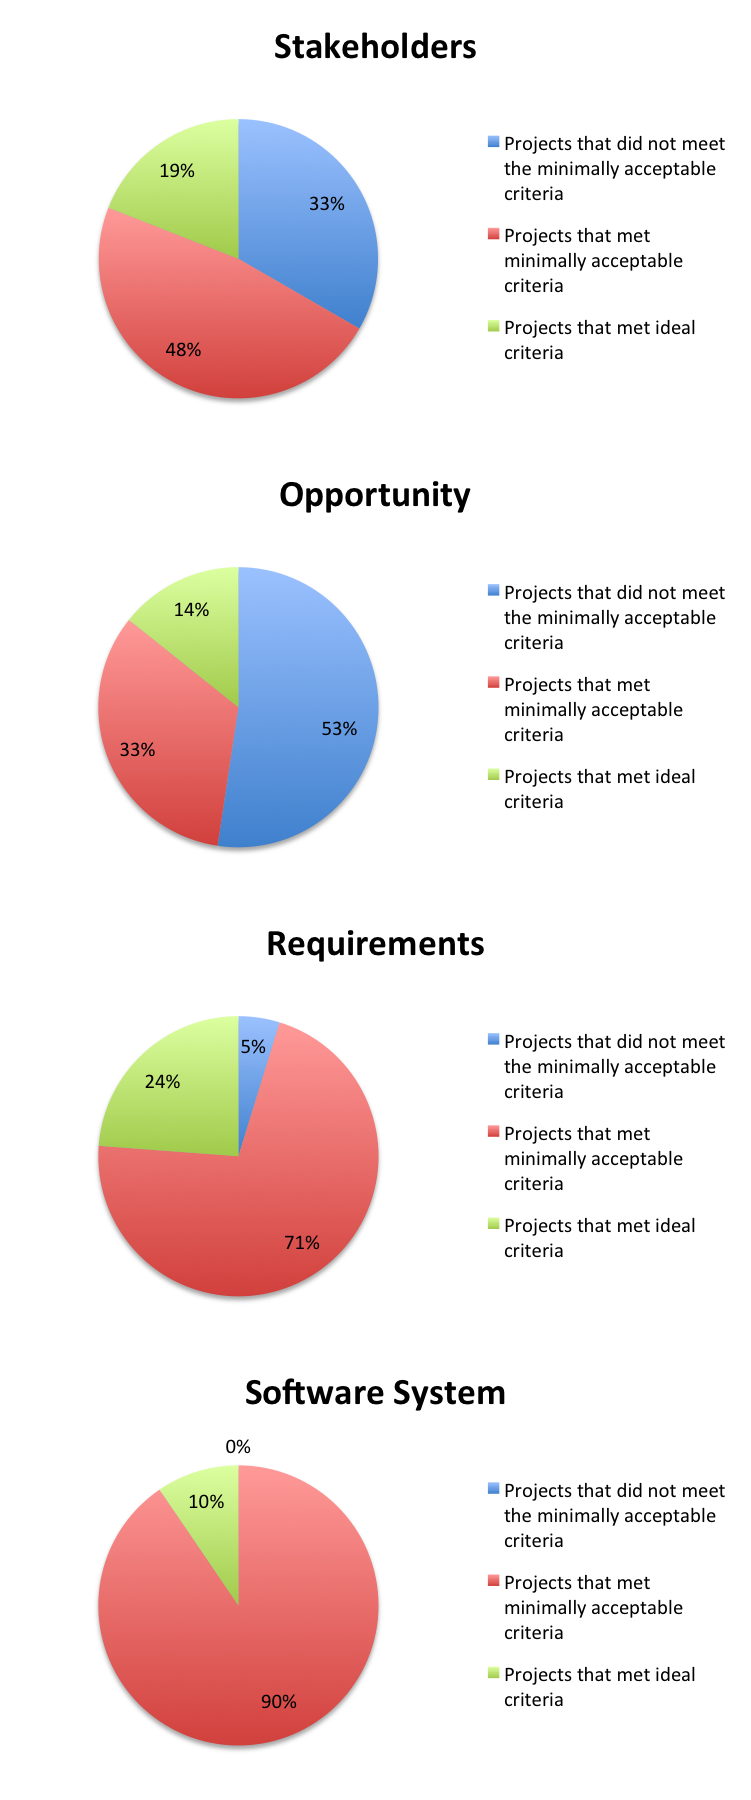
\includegraphics[width=3.45in]{essence_green_lighting_images/ProposalAlphasChartsStacked.png}
\caption{Essence Alphas checked for a proposal and circled for green-lighting project state}
\label{ProposalChart}
\end{figure}


In summary, we identified that 19\% of the proposals had represented
\textbf{Stakeholders}, 14\% of the proposals established the business value
of the \textbf{Opportunity}, 95\% \footnote{95\% is all the projects minus the 5\% that did not achieve any state} of the proposals captured the high level \textbf{Requirements} (and 24\% \footnote{24\% is the percentage of Bounded (19\%) and Coherent (5\%) projects} captured the project scope and success criteria), and 10\% of the proposals had defined criteria for selecting or identifying the \textbf{Software System} architecture. Since we do not expect the proposals to define architecture selection criteria, we are mostly concerned about the low
percentages for \textbf{Stakeholders} and \textbf{Opportunity} Alphas. Regarding
the \textbf{Requirements} Alpha, we would also like to increase the number of
proposals with defined project scope and success criteria.


\subsection{Research Question 2: What are some problems with the practicum that could potentially be mitigated to some extent prior to the start of the project?
}

While experimenting with Essence Reflection Meetings in the
context of practicum projects \cite{EASE2014, ICSE2014}, we
noticed that some practicum issues could potentially be identified and
addressed before the engagement started. These issues typically involve:

\begin{itemize}
\itemsep1pt\parskip0pt\parsep0pt
\item
  Missing stakeholder representation
\item
  Unclear opportunity value, and
\item
  Undefined project scope and success criteria
\end{itemize}

\textbf{Missing stakeholder representation:} Philosophical differences about
stakeholder representation present a challenge. The faculty believe that
most stakeholder groups should be represented and that a single
person cannot represent every stakeholder group because the groups
typically have very different needs. On one project, the team was building
a benchmark for comparing native code versus HTML5 code
on Android devices for the purpose of publishing the results to the
development community. While using the Essence framework for project
monitoring and steering \cite{ICSE2014}, the team
realized that no one represented the development community stakeholder
group. The team proactively interviewed local mobile developers and
presented the findings to the client. The client chose to ignore the
feedback putting at risk the potential benefit of the benchmarking
report to the development community. If a client is unwilling (or does
not understand the need) to have a representative for each (or most)
stakeholder groups, then the Request for Proposal process should
identify this issue and we can discuss our perspective with the client. If
the client is unwilling to change, we can decide to reject the
proposal.

\textbf{Unclear opportunity value and undefined project scope and success
criteria:} On a few projects, the teams spent the first two to three
weeks identifying the underlying problem and
analyzing the market trends and competitive landscape to validate the
need for a solution. Then they spent more iterations agreeing on the
project scope and success criteria. While this is an interesting
exercise, this significantly delayed the implementation work so the teams delivered substantially less functionality than the other
teams. Establishing the value of the opportunity and potentially
defining the project scope and success criteria at the start of the
practicum would have provided the practicum teams enough time to
build an interesting solution.

We believe that improving ``project readiness'' enhances the student experience, which remains to be verified in future research. If the stakeholder groups are not represented, then the
client can find representatives prior to the start of the project. If a client cannot clearly articulate the opportunity, the project's
benefits, the project's scope, or the project's success criteria, then
we can accept other proposals that have a larger impact.

Addressing these issues prior to the start of the practicum would
better align the expectations of the client with our educational goals, give the students a richer experience, provide more value to the client, and further the impact of the university.

\subsection{Research Question 3: From the faculty perspective, what should be the minimum or ideal initial state of a project?}

\begin{table*}
\renewcommand{\arraystretch}{1.3}
\caption{Green-lighting project state for each Essence Alpha (CMU1.1)}
\label{GreenLightingProjectState}
\begin{tabular}{|l|p{2.50in}|p{3.35in}|}
\hline
\textbf{Alpha}  & \textbf{Minimally acceptable}       & \textbf{Ideal}                        \\ \hline
Stakeholders    & \textbf{Recognized (Partial)}       & \textbf{Represented (Partial)}        \\ 
                & (check) Possible stakeholder groups are identified & (check) Stakeholder representatives are appointed \\
                & (not) Team agrees on relevant stakeholder groups & (check) Stakeholder representatives agree to take on responsibilities \\
                & to be represented                 & (not) Stakeholders agree on collaboration approach \\
                & (not) Responsibilities of stakeholder representatives  & (not) Representatives respect team's way of working \\
                & are defined                         & (check) Stakeholder representatives empowered to take on responsibilities \\ \hline
Opportunity     & \textbf{Solution Needed (Complete)} & \textbf{Value Established (Complete)} \\[5ex] \hline
Requirements    & \textbf{Conceived (Complete)}       & \textbf{Bounded (Partial)}            \\
                &                                     & (check) Purpose and extent of system are agreed \\
                &                                     & (check) Success criteria are clear \\
                &                                     & (not) Processes and tools for handling requirements are in place \\
                &                                     & (check) Scope constraints are identified \\
                &                                     & (not) Assumptions made while defining requirements are captured \\ \hline
Software System & None                                & \textbf{Architecture Selected (Partial)} \\
                &                                     & (check) Criteria for selecting architecture are agreed \\
                &                                     & (check) Platforms, technologies, languages are selected \\
                &                                     & (check) Selected architecture addresses key technical risks \\
                &                                     & (check) Buy, build, reuse decisions are made \\
                &                                     & (not) Stakeholders agree on necessary documentation \\
                &                                     & (not) Stakeholders agree on support service levels \\
                &                                     & (check) Non-functional architectural characteristics are considered \\ \hline
\end{tabular}
\end{table*}

After reviewing the practicum proposals and reflecting on practicum
issues listed in \textbf{Research Question 2}, we created green-lighting project
states for each Essence Alpha documented in Table~\ref{GreenLightingProjectState}.

The existing literature \cite{EssenceBook} implies
that staging (green-lighting in our case) can be done at the Alpha state level. In the process of creating our green-lighting project states, we discovered that for some of the Alpha states, we could not select all the checklist items in the entire state. For example, at the proposal stage, we do not expect responsibilities of the stakeholder representatives to be defined; this happens through a conversation between the team and the stakeholder representatives. In creating the green-lighting project state, we ignored some checklist items thus creating partial Alpha states.

The minimally acceptable and ideal states were defined with the goal of mitigating the problems identified in the previous research question, and based on the researchers expertise. Further work is necessary to validate the proposed states for each Alpha in the context of our practicum projects. Note however that other project courses might require different sets of minimally acceptable and ideal states to better address their specific needs.

\subsection{Research Question 4: How do the proposals
compare against the proposed minimum and ideal green-lighting project
states?}

Now that we have evaluated the proposals (Step 1) and created the
green-lighting project states (Step 2), we identify which proposals
meet the green-lighting criteria (Step 3 of the Green-lighting Approach). 

Table~\ref{table_proposal_evaluations} shows the proposals from the Spring 2014 and Summer 2014 semesters that meet the minimally acceptable and ideal criteria for green-lighting. 

\begin{table}
\renewcommand{\arraystretch}{1.3}
\caption{Proposals compared to green-lighting project states}
\label{table_proposal_evaluations}
\begin{tabular}{|p{1.10in}|p{0.95in}|p{0.95in}|}
\hline
Alpha & Number of projects that met minimally acceptable criteria & Number of projects that met ideal criteria \\ \hline
Stakeholders & 14 out of 21 & 4 out of 21 \\ \hline
Opportunity & 10 out of 21 & 3 out of 21 \\ \hline
Requirements & 20 out of 21 & 5 out of 21 \\ \hline
Software System & 21 out of 21 & 2 out of 21 \\ \hline
All (Satisfies all Alphas) & 8 out of 21 & 0 out of 21 \\ \hline
% Overall (Across all Alphas) & 8 out of 21 & 0 out of 21 \\ \hline
\end{tabular}
\end{table}

This analysis revealed a gap between the proposals and our
expectations, specifically in regard to representing stakeholders and
establishing the value of the opportunity. None of the proposals matched our ideal criteria across all Alphas, while 8 out of 21 satisfied our minimal expectation.

Around one third of the proposals did not have appropriate
representation for different stakeholder groups. In these proposals, the
client themselves would define, prioritize and validate the needs of the
different stakeholders groups. In our experience, when a team finishes
this kind of project, there is a high probability that the solution
would not deliver sufficient value for each stakeholders group. In some
cases, the solution may be unusable.

Around half of the proposals did not clearly state the
opportunity. The proposals described the problem to be solved, but did
not articulate the benefit of solving the problem. In a few cases, we
suspect the client has found a ``solution'' but has not yet identified
the problem to solve. In our experience, at the end of the project,
the project would be ``successful'' in delivering code to the client,
but might not solve a real world problem. Alternatively, the client
might have a detailed understanding of the opportunity, but may have not
clearly communicated that opportunity in the proposal.

The current proposals contain the same issues as the previous practicums identified in Research Question 2. The Green-Lighting Approach surfaced that the current proposals could repeat the problems identified in the past.


\subsection{Research Question 5: Do we need to
improve the Request for Proposal?}

In observing the gap between the proposals and our desired minimal
state, we wondered if asking different questions would help the sponsors
to record the kind of information that we need. Since the proposal's
content is a proxy for the sponsor's knowledge, is it possible that the
sponsor has more detailed knowledge that is not recorded in the proposal?
In addition, simply asking a question might cause the client to do some
groundwork not originally considered, which could potentially move the
project to a higher initial state. 

While analyzing the proposals, we had difficulty determining the stakeholder groups in the
 \textbf{Stakeholders} Alpha, the projected value of software system in the
 \textbf{Opportunity} Alpha, the list of high-level features that captures
the system purpose in the \textbf{Requirements} Alpha, and the non-functional
architectural characteristics in the \textbf{Software System} Alphas. The
Request for Proposal does not clearly ask for this information. We need
to ask specific questions to determine if the client can articulate the
answers. Improving the Request for Proposal would also facilitate
easier analysis for these aspects.

In order to help ascertain this information, we asked the sponsors four
questions.

{Survey Question 1. List your stakeholder groups and identify who will be
representing each group. (Note: Ideally there should be a different
person representing each group.)}

In examining the free-text answers, about \sfrac{2}{3} of the sponsors listed
out different stakeholder groups. A few even named who would fulfill the
role. One third of the sponsors listed themselves as the primary and
only stakeholder. In reviewing the proposals, these sponsors are not the
target stakeholder groups. This suggests that these proposals could be
misaligned with our educational goals of involving every stakeholder
group in the process.

{Survey Question 2. What value would the stakeholders receive from a successful engagement? If possible, please quantify the value (e.g. monetary
value, social return).}

In examining free-text answers, about half of the respondents were not
able to articulate the opportunity of the proposal. The other half of
the respondents appealed to social returns such as improving the
emergency response situations which could save lives and reduce injuries
or connecting seniors to their families and caregivers. None of the
respondents were able to put a monetary value to the opportunity.

{Survey Question 3. What features would you like to see implemented during the
practicum? }

In reviewing the free-text answers, about half of the sponsors provided
a feature list. The other half provided vague answers to the question.
This question needs to be rephrased. Perhaps asking the client to
prioritize the features to be delivered would be more effective.

{Survey Question 4. What are the key non-functional requirements (e.g.
scalability, security, performance, etc) that the solution should
satisfy?}

Most of the sponsors were able to clearly articulate the quality
attributes needed for the project. One sponsor said, ``Software will be
written in C/C++, documented well and reusable.'' 

When the answer does not fully or properly articulate the
non-functional requirements of the system, we recommend that the course
owner interviews the sponsor to acquire this information. 

The results from questions 1 and 2 are consistent with our assessment
of the proposals from Research Question 1. Adding these questions would
facilitate analysis but might not cause the sponsors to change the
stakeholder representation. Additional conversations between the course 
owner and the sponsor might be necessary.

Based upon these results, we plan to add questions 1, 2, and 4 to our
Request for Proposal. We will continue to experiment to find a question
that elicits a list of high-level features. These improvements to
our Request for Proposal will help us better assess the initial states
of the proposals.

% \subsection{Research Question 6: What is the effect of
% using the Essence Green-lighting Approach on the time it takes to accept
% or reject a project?}

% With modifications to the Request for Proposal questions, we believe
% that the Essence Green-lighting Approach would structure, simplify, and
% reduce the amount of time it takes to accept or reject a proposal when compared to our current process.
% However this remains to be verified.

In the current Request for Proposal process, the course owner reads
through each proposal to verify its completeness. We noticed that
clients submit ad-hoc proposals without necessarily following the
provided guidelines in terms of structure and content. This makes
assessing the readiness of each proposal arduous. The Request for
Proposal process provides a non-editable document and asks the sponsor
to address the items listed in Section
\ref{ProposalQuestions}. We recommend replacing this
document with a restructured editable template where the sections are
clearly aligned to the four Essence Alphas. Clients would be asked to
fill-in the sections of this template. 

% With the proposed Green-lighting Approach, the course owner still needs
% to read through each proposal, but instead of looking for completeness,
% the course owner assesses the four Essence Alphas in the green-lighting
% project state. This requires the small additional effort of reading
% through at most 23 checklist items, and even less if the proposals are
% less mature. These changes would reduce the time on task for the current
% verification for completeness of ad-hoc proposals by organizing the data
% provided by the client and simplifying the assessment of the
% green-lighting project states.

\subsection{Research Question 6: What are limits to
the approach and limitations to its effectiveness?}

\subsubsection{Green-lighting Approach does not factor important business considerations}
The approach provides data for a structured decision making process for
accepting and rejecting proposals, however, there might be reasons to
have a project go forward even though green-lighting says ``no.''
Several examples include paying clients, a high impact project, career
opportunity for students, and potential partnership for research
collaboration. While the approach provides a black and white answer,
we suspect that sound judgment is required for special circumstances.

\subsubsection{Green-lighting project states do not always
align to Alpha states}

In following the Green-lighting Approach, we discovered that partial
states, not Alpha states, represent our proposal acceptance criteria.
Some of the checklist items on one Alpha state would apply to accepting
a proposal and the rest of the checklist items would not. For example, 
for us to green-light a proposal, we would expect that the
proposal would meet the first checklist item of the
 \textbf{Stakeholders} \textit{Recognized} card, not the second or third as
described in Table \ref{GreenLightingProjectState}. 
Using partial states is possible but inconvenient. 

\subsubsection{Green-lighting Approach relies upon the Essence framework}
The Green-lighting Approach relies upon the Essence kernel for providing 
a systematic framework for evaluating proposals. The case study shows that  
only a subset of the framework is leveraged: Only 4 out of the 7 Alphas are 
relevant, and only the first few states (maximum 3) of each Alpha are necessary 
to green-light a project. In addition, some of the states need to be only partially 
considered as described in the previous section. Therefore, it is possible that a simpler checklist 
could be evolved, rather than relying upon the Essence framework. The extra 
complexity could be justified however if the project team continues to use 
the Essence framework during development to leverage mechanisms like progress 
monitoring and project steering. In that case it might make sense to use the 
same framework throughout the project.

\subsubsection{Green-lighting Approach does not guarantee project success}
Given the variety of issues that can emerge from a student project experience, and the fact that the initial state has only a limited impact on the overall project, the Green-Lighting Approach is not a silver bullet that will solve all team-based issues.
Only some risks might be reduced by systematically examining each proposal to identify
potential problems that the instructor could solve, mitigate against, 
or simply decide not to deal with by rejecting the proposal.

\subsection{Threats to Validity}
Internal Validity: This work assumes that it is desirable to filter
proposals and that is is possible to select proposals that will better achieve the
practicum goals listed in Section \ref{Introduction}. It could be the case
that a rejected proposal would have more significant learning
opportunities for the students than an accepted proposal.

Experimenter bias: We each had one years worth of experience in working with
the Essence framework prior to the start of this research. It is
possible that someone with less experience may encounter different results.

\section{Conclusions and Future Work}
\label{Conclusion}

This paper presents a first attempt to characterize and study a project 
selection process in academia. We proposed a Green-lighting Approach using the Essence framework and
applied the approach to the Request for Proposal process for the
practicum course at Carnegie Mellon University in Silicon Valley. 

After receiving and reviewing a set of proposals, the faculty determined each 
proposal state for each Essence Alpha. Based upon these initial states, prior experience, 
and recent problems, we created a gating function called green-lighting project
state to screen out proposals that are not ready for student teams.

After creating the green-lighting project state for each
Essence Alpha, we realized that our current Request for Proposal did
not prompt the clients to provide enough detail about the stakeholder
representations, the projected value of the opportunity, the project
scope and success criteria, and non-functional architectural
characteristics of the software system. We created draft 
questions and then tested the new questions with the prospective
clients. We recommend modifying our Request for Proposal to include
an editable template structured around the Essence Alphas and to include
several of the new questions identified in this paper. 

Further research is necessary to validate our green-lighting project state 
as well as our modified Request for Proposal. 
Even though green-lighting projects does not guarantee project success, 
the goal is to reduce risks by systematically examining each proposal to identify
potential problems that the instructor could solve, mitigate against, 
or simply decide not to deal with by rejecting the proposal.
More work is necessary to verify that our approach helps us reach that goal.

Using the Essence framework for green-lighting practicum projects in academia presents some limitations. 
First, the approach does not explicitly factor in business forces that affect proposal selection. 
Second, the Essence framework might be overly complex for green-light practicum projects, 
as only a subset of the Essence framework is necessary to perform the task.
In addition, the need to split the checklist items on the Alpha states to represent green-lighting 
project states prevents us from using the Essence cards out of the box hence losing the simplicity of the cards.

Still, project courses that use the Essence framework during development (to leverage mechanisms such as progress 
monitoring and project steering \cite{ICSE2014}) might want to borrow some ideas from the proposed Green-Lighting Approach, 
as it might make sense to leverage the same framework throughout the project.
In that case, we recommend customizing the approach by defining minimally acceptable and ideal states based on the course specific needs. 

For project courses that are not planning on using Essence during development, 
the framework could still be used as an inspiration for deriving simple custom green-lighting checklists for various project dimensions. Better aligning client proposals and educational goals has the potential of enhancing the students learning experience.


% Sample apostrophy's to remove team's 


\newpage
\section*{Abstract}
\textit{Context:} Software development is a complex socio-technical endeavor that involves coordinating different disciplines and skill sets. Practitioners experiment with and adopt processes and practices with a goal of making their work more effective.


\textit{Objective:} The purpose of this research is to observe, describe, and analyze software development processes and practices in an industrial setting. Our goal is to generate a descriptive theory of software engineering development, which is rooted in empirical data.


\textit{Method:} Following Constructivist Grounded Theory, we conducted a two-year five-month participant-observation of \numberOfObservedProjects{} software development projects at Pivotal, a software development company. We interviewed \numberOfInterviews{} software engineers, interaction designers, and product managers, and analyzed one year of retrospection topics. We iterated between data collection, data analysis and theoretical sampling until achieving theoretical saturation and generating a descriptive theory.


\textit{Results:} 1) This research introduces a descriptive theory of Sustainable Software Development. The theory encompasses principles, policies, and practices aiming at removing knowledge silos and improving code quality (including discoverability and readability), hence leading to development sustainability. 2) At the heart of Sustainable Software Development is team code ownership. This research widens the current definition and understanding of team code ownership. It identifies five factors that affect ownership. Developers achieve higher team code ownership when they understand the system context, have contributed to the code in question, perceive code quality as high, believe the product will satisfy the user needs, and perceive high team cohesion. 3) This research introduces the first evidence-based waste taxonomy, identifying eight wastes along with causes and tensions within wastes. It also provides a comparison with the taxonomy of wastes found in Lean Software Development.


\textit{Limitations:} While the results are highly relevant to the observed company, Pivotal, the outcomes might not apply to organizations with different software development cultures.


\textit{Conclusion:} The Sustainable Software Development theory refines and extends our understanding of Extreme Programming by adding new principles, policies, and practices (including Overlapping Pair Rotation) and aligning them with the business goal of sustainability. One key aspect of the theory is team code ownership, which is rooted in numerous cognitive, emotional, contextual and technical factors and cannot be achieved simply by policy. Another key dimension is waste identification and elimination, which has led to a new taxonomy of waste. Comparing this taxonomy to Lean Software Development's list of wastes revealed our taxonomy's parsimony and expressiveness while illustrating wastes not covered by previous work. Overall, this research contributes to the field of software engineering by providing new insights, rooted in empirical data, into how a software organization leverages and extends Extreme Programming to achieve software sustainability.














\chapter{Introduction}
\label{IntroductionChapter}


Imagine that you are a Vice President of a multi-million dollar software development business unit managing 100 software engineers and 20 product managers. You have 25 teams working on various interrelated software products. The entire organization balances 1) adding new features to the next release, 2) solving customer escalations from installed products, and 3) handling maintenance chores such as routinely upgrading dependencies. Over the last few releases, you have seen a continuing decrease in your teams' productivity, and a steep increase in complaints from customers related to product quality. And somehow, there is never enough time to address those challenges.


In the middle of all this, one team is extremely difficult  to manage. The team is composed of highly skilled software engineers. They write well tested, clean code. The test suite is slow, but is thorough and catches issues before they get to the customer. 


The team resists collaborating with other teams or customers. The team developed an \quotes{us versus them} or \quotes{us versus management} attitude. Their product manager would like the team to be in the office more often to increase collaboration. While the organization expects teams to be in the office during core business hours, this team believes that as long as the work gets done, nobody should care where or when they accomplish the work. The product manager is growing frustrated with the team's attitude about features. Their focus appears to be on delivering something that works without truly understanding how the features should work. As a result, when they deliver code, the implementation does not always solve the customer's needs or works the way the customer expects. 


How did software development come to this? Why is software development so hard? Why is collaboration so difficult? How can we build teams that embrace collaboration, help others solve the problems, and train others to do their work?


The complexities of software development emerge, in part, due to 1) uncertainty about product to market fit resulting in changes to the feature set during and after development, 2) constantly changing dependent technologies, 3) the challenge of maintaining legacy code, 4) the lack of physical constraints resulting in boundless solutions, 5) measuring progress is challenging because project scope is a moving target and bringing visibility to an intangible process is difficult, and 6) software is written by people having various expertises as well as social and technical skills. Teams require coordination and collaboration. Building high performing teams requires effort and care. Unlike assembly line work, engineers are not fungible. Even if two engineers have the same competency in a set of technologies, their individual temperaments and personalities affect team dynamics. Building software is challenging. 


While it appears that any set of processes will work for tiny teams in the short term, creating an engineering culture where large teams deliver value week after week, month after month regardless of team disruption and changing circumstances is no easy task. Any company that achieves proficiency in software development becomes an interesting research opportunity. We choose Pivotal because it is successful; it is unusual in its continued use and evolution of Extreme Programming \cite{BeckExtremeProgramming2004};  it is accessible and cooperative with research. Chapter \ref{ResearchContextChapter} describes Pivotal, our research context. 


In order to understand how Pivotal develops software, we employed Constructivist Grounded Theory as the research method. Chapter \ref{ConstructivistGroundedTheoryChapter} describes Constructivist Grounded Theory and Chapter \ref{ResearchMethodChapter} describes our data sources and particular use of Grounded Theory. This study had an unusually ambitious scope. In many Grounded Theory studies, the researcher spends a few weeks interviewing participants and analyzing data. Here, one researcher spent \durationOfResearchStudyPlural{} working with participants 5 days per week on \numberOfObservedProjects{} teams. 


Applying Grounded Theory at Pivotal unearthed the theory of Sustainable Software Development, an explanation on how Pivotal teams can thrive despite team disruption and successfully deliver software to their stakeholders. Chapter \ref{SustainableSoftwareDevelopmentChapter} describes the theory's principles, policies, and practices. The theory explains how teams survive disruption by actively removing knowledge silos and caretaking the code. At the heart of the Pivotal process is team code ownership. Many of Pivotal's practices have the effect of promoting team code ownership while removing individual code ownership. Chapter \ref{TeamCodeOwnershipChapter} identifies five factors that affect the team's sense of code ownership and explains why psychological ownership causes some engineers to struggle with the transition from individual code ownership to team code ownership. 


The Grounded Theory study also identified that Pivotal teams actively detect and remove waste. Since software development is an organic and messy problem space, finding all kinds of waste is no surprise. Chapter \ref{SoftwareEngineeringWasteChapter} conducts the first empirical research study into a waste taxonomy and contrasts it with Lean Software Development's waste taxonomy. \sout{Some of the wastes types, such as \quotes{unnecessary cognitive effort,} are rarely salient unless one is specifically looking for them.}


Chapter \ref{ConclusionChapter} discusses future research and concludes the research study. 


Appendix \ref{AppendixChainOfEvidence} provides the chain of evidence for the waste taxonomy after iteratively applying constant comparison. 


Appendix \ref{AppendixInterviews} showcases interview data. The initial interviews began with the question, \quotes{draw your view of Pivotal's software development process.} The appendix includes a sample of these drawings with interview transcript snippets where the interviewee describes the drawing. Once team code ownership emerged as a core category, many interviews began with the question, \quotes{draw how you feel about the code.} Section \ref{AppendixFeelAboutTheCode} provides some of these drawings. When the pictures are not obvious, a brief narrative explains the illustration.


% opportunities to remove waste are apparent even for companies that actively remove waste. 


\chapter{Extreme Programming}
Extreme Programming is characterized by a set of values, principles, and practices. When transitioning to Extreme Programming, Beck recommends adopting the primary practices first. 
\section{Values}
\textbf{Communication:} Extreme programming is a collaborative endeavor with communication frequently happening. Teams prefer open and transparent communication. 
\quotes{You can listen to people who have had similar problems in the past} \cite{BeckExtremeProgramming2004}. When combined with the reflective principle, the team can ask \quotes {what communication do you need to keep yourself out of this trouble in the future?} \cite{BeckExtremeProgramming2004}


\textbf{Simplicity:} The team strives to \quotes{make a system simple enough to gracefully solve only today's problem} \cite{BeckExtremeProgramming2004}. Teams prefer simpler solutions to more complex solutions. Simpler solutions often take more work to discover and implement than complex solutions, but simpler solutions often require less communication than complex solutions.










\textbf{Feedback:} Feedback provides an opportunity for the team to respond to changing circumstances in the marketplace, in the product, in the team, and with the development process. Change requires feedback. In order for continuous improvement to work, the team decides to collect feedback at multiple frequencies and at multiple levels. The team prefers improvement over expecting perfection. Teams attempt to shorten the feedback cycle so that the team can respond sooner rather than later.


\textbf{Courage:} \quotes{Courage is effective action in the face of fear}   \cite{BeckExtremeProgramming2004}. Sometimes it takes courage to make the needed change. Messy code will remain messy unless someone has the courage to make it better. With change, the team needs to accept the risk that the system may break. The individual considers the consequences before making changes. When the team knows the problem, courage is a bias to action. When the team does not know the underlying problem, courage may be patience. 


\textbf{Respect:} Collaborative software development is founded on respect. Team members decide to respect each other. \quotes{If members of a team don't care about each other and what they are doing, XP won't work} \cite{BeckExtremeProgramming2004}.


\textbf{Others:} Teams may adopt additional values and align their practices around the values. 


\section{Principles}
\textbf{Humanity:} The practices that a team follows need to satisfy human needs. Alternative software development practices may not respect psychological needs. In this case, a practice may grind away at an individual's humanity \cite{BeckExtremeProgramming2004}. Beck lists fundamental needs as basic safety, accomplishment, belonging, growth, and intimacy \cite{BeckExtremeProgramming2004}. Team software development balances the needs of the individual with the needs of the team. 


\textbf{Economics:} People buying the product fuels the business. The practices that a team follows need to balance business needs with technical needs\quotes {Software development is more valuable when it earns money sooner and spends money later} \cite{BeckExtremeProgramming2004}. Incremental design and incremental delivery allows the team to release earlier and delay expenses until later. Avoid building a \quotes{perfect} product that one wants to buy.


\textbf{Mutual Benefit:} The practices that a team follows need to find solutions that benefit everyone involved. A practice that does not benefit the team now is not mutually beneficial, e.g. writing documentation for a faceless maintenance team. Mutual beneficial practices benefit people now and the future. 


\textbf{Self-Similarity:} Try applying solutions that work in one context to another context. Beck sees similarity in listing themes for a quarter, addressing stories in a week, writing tests for a story.


\textbf{Improvement:} Teams benefit from constant improvement. The practices that a team follows evolve and improve over time. The point of XP is \quotes{excellence in software development through improvement} \cite{BeckExtremeProgramming2004}. Starting is prefered to waiting for perfection. 


\textbf{Diversity:} Multiple perspectives provides richer solutions. \quotes{Two ideas about a design present an opportunity, not a problem}  \cite{BeckExtremeProgramming2004}. The practices that a team follows should resolve conflict productively. Teams benefit from diversity of skills, perspectives, attitudes, and experiences.


\textbf{Reflection:} Teams reflect on how and why they are working. The practices that a team follows should enable reflection at different frequencies and multiple levels. Mistakes are seen as opportunities for growth.


\textbf{Flow:} \quotes{Flow in software development is delivering a steady flow of valuable software by engaging in all the activities of development simultaneously}  \cite{BeckExtremeProgramming2004}. The practices that a team follows should decrease batch sizes to enhance flow. Teams want a steady stream of work moving through the system. The ideal \quotes{batch size} is one story per developer. Anything that interrupts the stream of work needs removing. 


\textbf{Opportunity:} The practices that a team follows need to frame problems as opportunities. A team \quotes{playing it safe} will make less mistakes but also move slower than needed.


\textbf{Redundancy:} \quotes{The critical, difficult problems in software development should be solved several different ways} \cite{BeckExtremeProgramming2004}. The practices that a team follows should address diffult problems in mulpitle ways. For example, XP handles the critical, difficult problem of defects with \quotes{pair programming, continuous integration, sitting together, real customer involvement, and daily deployment}  \cite{BeckExtremeProgramming2004}. 


% The team needs to continue in spite of team disruption. Spreading knowledge around the team helps it survive through churn. This enables people to go on vacation whenever needed.


\textbf{Failure:}


\textbf{Quality:}




\textbf{Baby Steps:} Start with the simplest smallest change possible and grow from there


\textbf{Accepted Responsibility:} The team is responsible for the system. 




People tend to act as if everyone else was like them with similar preferences. People are different and the
\quotes{If you want to travel fast, travel alone. If you want to travel far, travel in a group.}


\section{Primary Practices}
\textbf{Sit Together:}
\textbf{Whole Team:}
\textbf{Informative Workspace:}
\textbf{Energized Work:}
\textbf{Pair Programming:}
\textbf{Stories:}
\textbf{Weekly Cycle:}
\textbf{Quarterly Cycle:}
\textbf{Slack:}
\textbf{Ten-minute Build:}
\textbf{Continuous Integration:}
\textbf{Test-First Programming:}
\textbf{Incremental Design:}








\section{Corollary Practices}
\textbf{Real Customer Involvement:}
\textbf{Incremental Deployment:}
\textbf{Team Continuity:}
\textbf{Shrinking Teams:}
\textbf{Root-cause analysis:}
\textbf{Shared Code:}
\textbf{Code and Tests:}
\textbf{Single Code Base (branches live a few hours at most):}
\textbf{Daily Deployment:}
\textbf{Negotiated Scope Contract:}
\textbf{Pay-per-use:}




















\chapter{Research Context}
\label{ResearchContextChapter}


\section{Pivotal Labs}
Pivotal Labs is a division of Pivotal\textemdash a large American software company (with 17 offices around the world). Pivotal Labs provides teams of agile developers, product managers, and interaction designers to other firms. Its mission is not only to deliver highly-crafted software products but also to help transform clients' engineering cultures. To change the client's development process, Pivotal combines the client's software engineers with Pivotal's engineers at a Pivotal office where they can experience Extreme Programming \cite{BeckExtremeProgramming2004} in an environment conducive to agile development. 


Typical teams include six developers, one interaction designer, and a product manager. The largest project in the history of the Palo Alto office had 28 developers while the smallest had two. Larger projects are organized into smaller coordinating teams with one product manager per team and one or two interaction designers per team.


Interaction designers identify user needs predominately through user interviews; create and validate user experience with mockups; determine the visual design of a product; and support engineering during implementation. Product managers are responsible for identifying and prioritizing features, converting features into stories, prioritizing stories in a backlog, and communicating the stories to the engineers. Software engineers implement the solution. 


Pivotal Labs has followed Extreme Programming \cite{BeckExtremeProgramming2004} since the late 1990's. While each team autonomously decides what is best for each project, the company culture strongly suggests following all of the core practices of Extreme Programming, including pair programming, test-driven development, weekly retrospectives, daily stand-ups, a prioritized backlog, and team code ownership. We only observed teams at Pivotal Labs. Other teams, especially teams in other divisions, might have a different culture and follow different software practices.


\section{Day in the Life}
Pivotal provides breakfast to promote engineers starting the day at the same time. Many engineers socialize with their coworkers while eating breakfast. 


Office stand-up begins at 9:06 am. Everyone gathers around in a large circle. The stand-up covers \quotes{new faces,} \quotes{helps,} \quotes{interestings,} and \quotes{events.} The office stand-up lasts a few minutes. The two people running stand-up send an email to the company with a summary of the brief meeting. People then disperse for their team's stand-ups.


Team stand-ups provide a synchronization point for the team. Small teams (under eight people) typically will review what each individual accomplished yesterday and discuss any blockers to finishing the work. Large teams discuss \quotes{interestings} and \quotes{helps.} Some teams use a whiteboard to track \quotes{parking lot} issues (items needing discussion during stand-up). After team stand-up, the engineers then decide \quotes{pairing}, who will pair program with who. 


The team then determines which pairs will use which computer. If there is work already in progress, the pair working on that work will use that machine. The development environments configured to be identical. Pairing continues until 12:30 pm when the team takes a lunch break. After lunch, pairing continues until 6:00 pm. 


While coding, the developers follow Test Driven Development (or Behavior Driven Development.) Tests are written first before determining the design or writing code. A failing test provides the developers with a short term goal. The rhythm is to start a story, refactor if necessary, write a small failing test, write just enough code to get the test to pass, refactor if necessary, and repeat by writing a small failing test. The ideal flow is quick, short cycles of Test Driven Development. When a pair finishes their work, they start the next story at the top of the backlog. 


The product manager determines the features and the sequence of stories. The prioritization is kept in a backlog. The product manager decides \quotes{what} the product should do. The engineers determine the implementation details, \quotes{how} the code should be written to accomplish the task in the story. The product manager changes the direction of the product at any point in time by resequencing the backlog. The product manager does not change any \quotes{in-flight} stories (stories that the developers are working on.)


During each week, the team holds an iteration planning meeting. The product manager and designer communicate to the engineers the upcoming work, building a shared understanding of the stories. The engineers communicate to the product manager the complexity and risk associated with each story.


At the end of each week, the team holds a retrospection meeting to examine what is working well for the team, what needs improvement, and determine any action items to accomplish the identified improvements.






\section{Software Development Culture}
\sout{When compared to other companies, Pivotal's software development culture is marked by a high degree of collaboration and constant improvement.}


\subsection{Collaboration}
\sout{The culture promotes collaboration by preferring synchronous communication, encouraging asking for help, interacting across disciplines, creating an ego-less environment, enabling team code ownership, rotating who works on each part of the system, and pair programming. Experienced engineers model the culture so that new Pivotal or client engineers learn a new way of working.}


\sout{\textit{Synchronous communication} enables a high bandwidth conversionation, where participants can quickly discuss and iterate on a topic. Asynchronous communication (e.g. email or instant messaging) introduces delays in responses, context switching, the overhead of preparing a message, and increased opportunities for messages to be misunderstood. Co-locating the team into the same aisle increases the opportunities for synchronous communication and impromptu team huddles.  Co-located teams typically have greater verbal and nonverbal communication compared to distributed teams. Daily standups provide inexpensive touch points for the team to synchronize and resolve issues. Teams prefer synchronous communication over asynchronous communication. }


\sout{Since \textit{asking for help} is a regular part of the day, welcoming interruptions is desirable. Asking another pair for help is a sign of respect as engineers enjoy that someone values their opinion. On teams with 10 or more engineers, it is possible for one pair to be interrupted too frequently. When the interruptions consume too much time, making forward progress on a story becomes challenging. }


\sout{Pivotal forms \textit{cross-functional teams} with software engineers, product managers, and interaction designers sharing a common goal. The \textit{balanced team} movement espouses the same philosophy as Pivotal. }


\sout{An \textit{egoless culture} is promoted through a meritocracy. The team wants the best solution for the product regardless of who presents ideas. There is no discussion or awareness about job titles or seniority. While the HR system has engineering levels for comparing compensations across the organization, in day-to-day practice everyone is on the same level. Pivotal has a flat engineering culture. The rotation of project roles also reinforces an egoless organization; an engineer leading a project today will be an individual contributor on the next project}. 


\sout{\textit{Enabling team code ownership} means empowering the team to be able to work on any part of the system. The pair rotation of engineers and the rotation the engineers through different parts of the system helps remove individual psychological ownership of the code and promote collective ownership. Ideally, anyone on the team can work on any part of the team's code.}


\sout{\textit{Pair programming} conditions individuals to work well with the rest of the team. A healthy pair programming dynamics is one comprised of listening, empathy, teaching, and learning. These characteristics then transfer from interactions with the partner on a pair to the rest of the team. The pair works on everything together from software development, asking for help, taking breaks, and attending meetings. When individuals are pulled into a project related meeting, they take their partner with them. Since the team desires to spread knowledge and context to the entire team, the team prefers for both to be involved instead of one person soloing. Pair programming can foster healthy habits that serve the entire team well.}


\subsection{Constant improvement}


\sout{The culture embodies constant improvement through tight feedback loops. The feedback loops help the teams identify and remove waste. Feedback loops happen at different frequencies (e.g. ad-hoc, daily, weekly), at different levels (e.g. individuals, team), and on different aspects (e.g. scenarios, mock-ups, features, code, and the product.)}


\sout{Here are some feedback loops employed at Pivotal:}
\begin{itemize}
  \item Daily standups
  \item Weekly retros
  \item Daily pair programming feedback for improving personal interactions
  \item User research for identifying user persona and user needs
  \item User validation for verifying product or features
  \item Usability testing for validating sketches and mock-ups
  \item Product managers accepting or rejecting a story for validating development work
  \item Tests for confirming successful code refactorings 
  \item Difficult to change code for revealing design problems
  \item Difficult to test component for exposing design problems
  \item Rework as feedback for features was not adequately described or not properly implemented
  \item Bugs as feedback for improving development process or testing strategy 
\end{itemize}


\sout{Ideal feedback is provided promptly so that the individual or team learn from the situation. Delaying course corrections delay the benefits. For example, one team had a ten-minute build which periodically annoyed them and slowed their development workflow down. On the last week of the project, the team examined the slowness of the build and realized that a simple resequencing of the tests could bring it down to three minutes. The pair lamented, \quotes{why didn't we do this sooner?} as they could have benefitted from the results throughout the project. }


\sout{On a typical project, there often are many things that can be improved. The art is in prioritizing which pain points to address first. }


\sout{The weekly retro becomes a \quotes{catch-all} event for identifying any possible team improvement. Pivotal retros are open, cathartic experiences for the team, managed with seasoned facilitators. }



% Sample apostrophy's to remove team's 

\chapter{Grounded Theory}
\label{ConstructivistGroundedTheoryChapter}
Constructivist Grounded Theory \cite{Charmaz} provides an iterative approach to data collection, data coding, and analysis resulting in an emergent theory. 

Grounded Theory immerses the researcher within the context of the research subject from the point of view of the research participants. As the research progresses, Grounded Theory allows the researcher to incrementally direct the data collection and theoretical ideas. The process provides a starting place for inquiry, not a specific goal known at the beginning of the research. As the researcher interacts with the data, the data influences how the research progresses and guides the research direction. When starting a Grounded Theory research study, the core question is, \quotes{what is happening here?} \cite{GlaserTheoreticalSensitivity}. The researcher can apply this question to a domain of study, for example, \quotes{what is happening at the studied organization when it comes to software?}

Charmaz encourages the researcher to follow this Grounded Theory strategy: \quotes{seek data, describe observed events, answer fundamental questions about what is happening, and then develop theoretical categories to understand it} \cite{Charmaz}.

\begin{figure}[t]
\centering
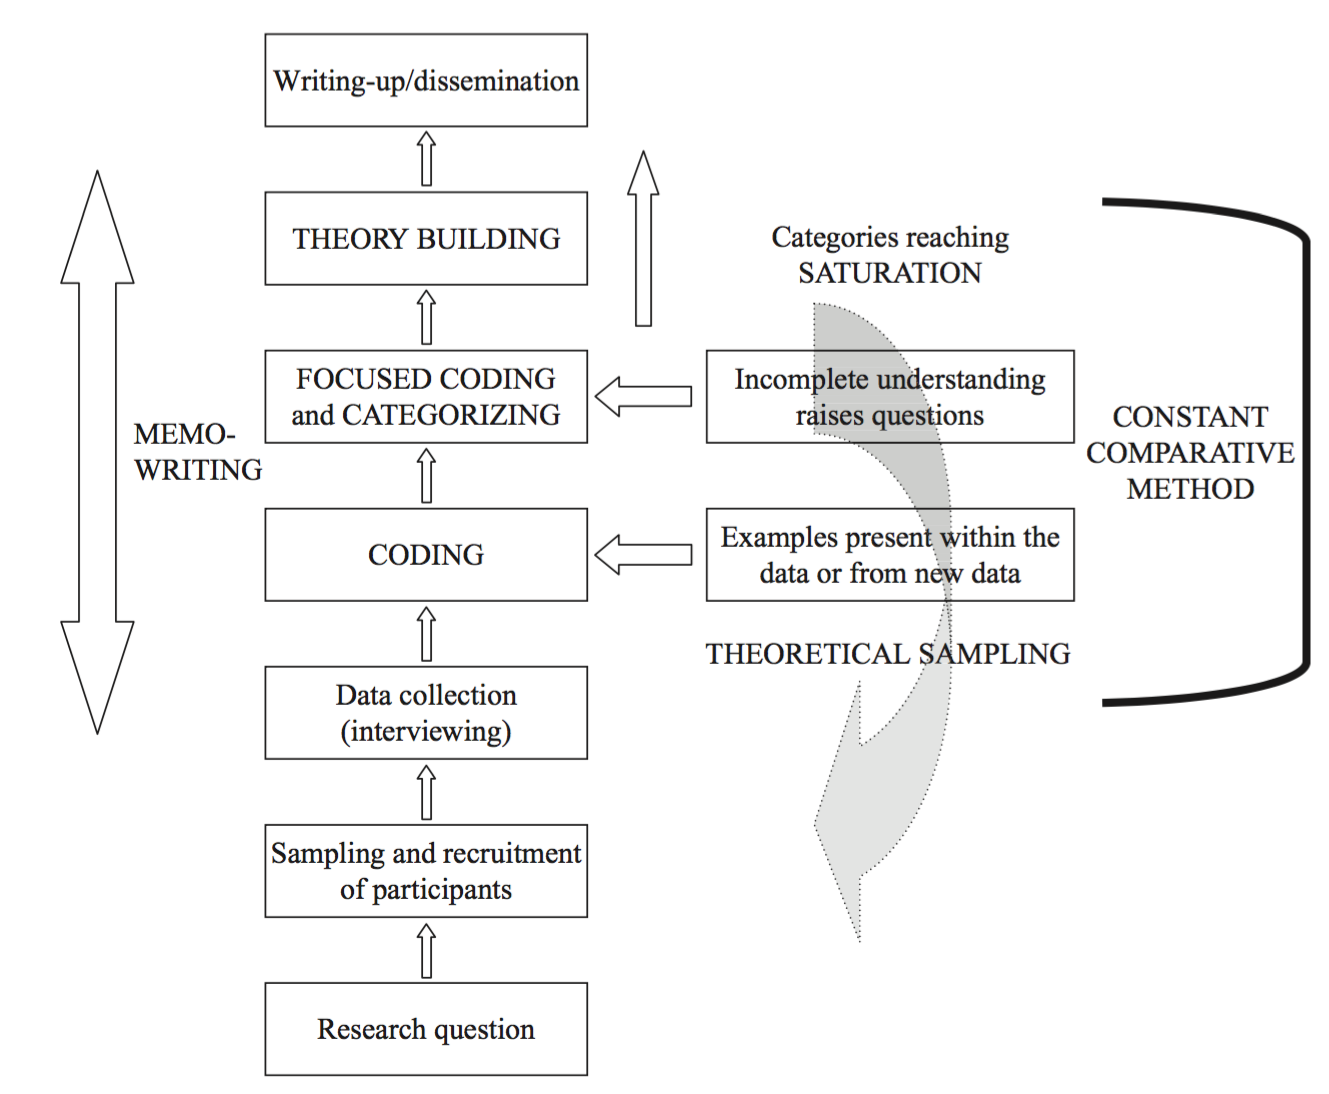
\includegraphics[width=6.4in]{grounded_theory_images/tweed_grounded_theory.png}
\captionof{figure}{Visualization of Grounded Theory by Tweed and Charmaz \cite{TweedGroundedTheory} }
\label{TweedVisualizationGroundedTheory}
\end{figure}

Grounded Theory follows an iterative process as illustrated in Figure \ref{TweedVisualizationGroundedTheory} \cite{TweedGroundedTheory}. After identifying a population to study, data is collected from interviews, participant observation, ethnographic study, or existing documents. Each kind of data, such as interviews, are coded and analyzed using constant comparison for the purpose of generating insights and recording memos. The coding process labels data with tags that emerge from the data. Constant comparison compares codes to codes for the purpose of identifying relationships between the codes. Memos are researcher diary notes. The principal activity is creating memos, and it supersedes and interrupts all other activities. The researcher sorts memos into a paper draft with data collection and analysis continuing until theoretical saturation occurs. If a new avenue of research arises,  additional data collection techniques are sometimes useful for generating the needed data. The data advances from the initial codes to focused codes, focused codes to core categories, and core categories to an emergent theory. 

%Research questions dictate which research methods are used. Charmaz argues that interviews are the best kind of data collection mechanism for certain kinds of research questions. (Todd: Need more detail)

Grounded Theory allows the addition of new aspects of the research while gathering data, which can even happen late in the analysis. The research question guides the data collection process, and the accumulation of knowledge alters the data collection process. It is common for early research to illuminate new angles. \quotes{Grounded Theory can give you flexible guidelines rather than rigid prescriptions} \cite{Charmaz}. The researcher's guiding interests can be used \quotes{as \quotes{points of departure} to form interview questions, to look at data, to listen to interviewees, and to think analytically about the data} \cite{Charmaz}.

There are three widely used versions of Grounded Theory: Classic Grounded Theory as championed by Barney Glaser \cite{GlaserDiscovery}, Straussian Grounded Theory as documented by Anselm Strauss and Juliette Corbin \cite{Strauss1988Basics}, and Constructivist Grounded Theory as described by Kathy Charmaz \cite{Charmaz}. 

Barney Glaser and Anselm Strauss invented Grounded Theory while performing the research for the \ul{Awareness of Dying} book \cite{GlaserAwarenessOfDying}. In response to associates asking for more details about the research process utilized in producing the novel results for \ul{Awareness of Dying}, Glaser and Strauss wrote \ul{The Discovery of Grounded Theory} \cite{GlaserDiscovery} in 1967. In 1988, Strauss and Juliet Corbin published \ul{Basics of Qualitative Research} \cite{Strauss1988Basics}. Glaser strongly felt that the book mischaracterized the approach, even asking Strauss to withdraw it from publication. Apparently, both authors had different points of view for what they invented. In a heated response, Glaser published \ul{Basics of Grounded Theory Analysis} in 1992 \cite{GlaserBasics} clearly differentiating his perspective from Strauss. \todo{In time, Glaser's approach became known as \quotes{Classic Grounded Theory} and Strauss's approach as \quotes{Straussian Grounded Theory.}} In time, several researchers evolved the approach using variations (such as recording an interview) that Glaser clearly describes as not part of Classic Grounded Theory. Furthermore, they switched from a positivist point of view to a constructivist perspective. One of these researchers, Kathy Charmaz, a Ph.D. student of Glaser, published \ul{Constructing Grounded Theory} in 2006 \cite{Charmaz}. 

\begin{figure}[h]
\centering
\captionof{table}{Stol's Grounded Theory Comparison}
\label{GroundedTheoryComparison}
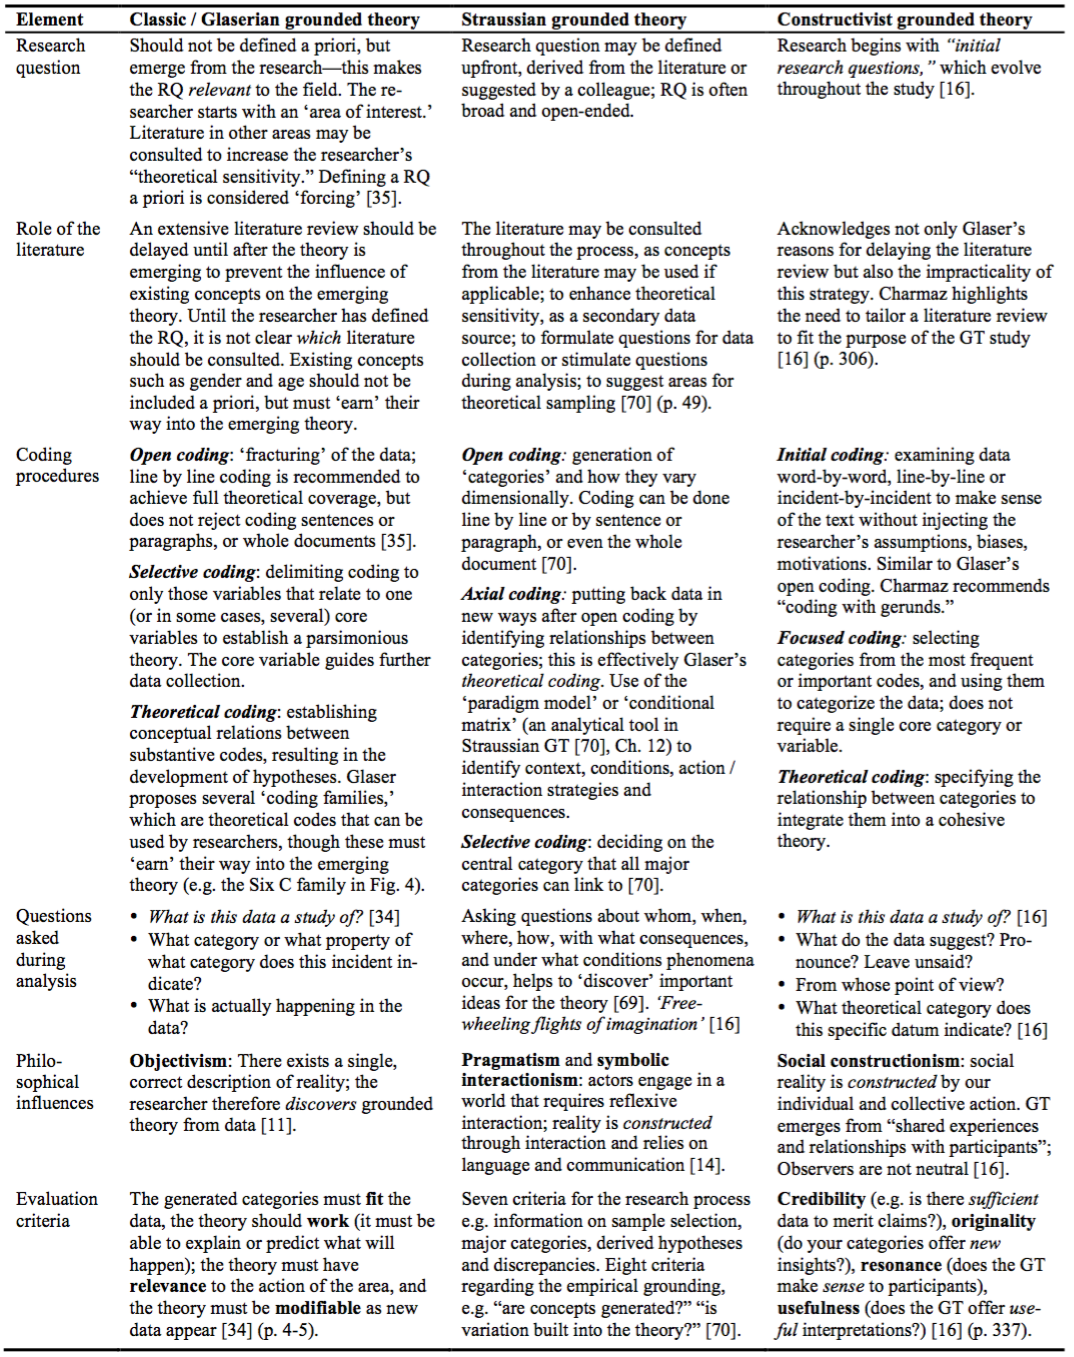
\includegraphics[width=6.4in]{grounded_theory_images/stohl_grounded_theory_comparison.png}
\end{figure}

Stol et al \cite{StolGroundedTheory} provide an excellent summary of the differences between the three types of Grounded Theory listed in Table \ref{GroundedTheoryComparison} shown at the end of this section. There are several significant differences which are summarized here:
\begin{itemize}
\item The influence of research questions: emerges from the research (Classic Grounded Theory), may be defined upfront (Straussian Grounded Theory), may be defined upfront and evolves through study (Constructivist Grounded Theory)
\item The role of existing literature: delayed in the process (Classic Grounded Theory), used when needed (Straussian Grounded Theory, Constructivist Grounded Theory)
\item Theoretical Coding (Classic Grounded Theory, Constructivist Grounded Theory) versus Axial Coding (Straussian Grounded Theory)
\item Analytic questions: \quotes{what is this data a study of?} (Classic Grounded Theory, Constructivist Grounded Theory), asking questions of the phenomena such as why, how, and when (Straussian Grounded Theory)
\item Philosophical differences: objectivism (Classic Grounded Theory), pragmatism (Straussian Grounded Theory), and social constructionism (Constructivist Grounded Theory)
\item Evaluation criteria
\end{itemize}


% \begin{table}[h]
% \centering
% \renewcommand{\arraystretch}{1.5}
% \caption{Concise comparison of Grounded Theory Approaches}
% \label{ConciseGroundedTheoryComparison}
% \begin{tabular}{|p{1.3in}|p{1.5in}|p{1.5in}|p{1.5in}|}
% \hline
%                                     & Classic Grounded Theory                                                                              & Straussian Grounded Theory                                  & Constructivist Grounded Theory                                                                      \\ \hline
% The influence of research questions & emerges from the research                                                                            & may be defined upfront                                      & may be defined upfront and evolves through study                                                    \\ \hline
% The role of existing literature     & delays use of literature in the process                                                              & use when needed                                             & use when needed                                                                                     \\ \hline
% Analytic coding                     & Theoretical Coding                                                                                   & Axial Coding                                                & Theoretical Coding                                                                                  \\ \hline
% Analytic questions                  & \quotes{what is this data a study of?}                                                             & hypothesizing as to causes of the data                      & \quotes{what is this data a study of?}                                                            \\ \hline
% Philosophical differences           & objectivism                                                                                          & pragmatism                                                  & social constructionism                                                                              \\ \hline
% Evaluation criteria                 & fits the data, works in explaining main concern, relevance to participants, modifiable with new data & Seven criteria for process and eight criteria for grounding & credibility (enough data), originality, resonance with participants, usefulness with interpretations \\ \hline
% \end{tabular}
% \end{table}


Classic Grounded Theory emphasizes action and process. It looks at the question, \quotes{what is going on here?} and decomposes it into \quotes{what are the basic social processes?} and \quotes{what are the basic social psychological processes?} \cite{Charmaz}.

Straussian Grounded Theory relies on Axial Coding as a key differentiator from Glaser's Theoretical Coding. Axial Coding is a systematic process for looking at the relationship between codes for aiding in the emergence of the theory. Axial Coding answers the questions \quotes{when, where, why, who, how, and with what consequences} \cite{Strauss1988Basics}. Glaser \cite{GlaserBasics} felt that axial coding favored the six C's  (Causes, Contexts, Contingencies, Consequences, Covariances and Conditions) one of the eighteen theoretical families identified in \ul{Theoretical Sensitivity} without allowing emergence of the other theoretical families \cite{GlaserTheoreticalSensitivity}. Charmaz prefers keeping codes \quotes{simple, direct, analytic, and emergent} instead of applying axial coding which can distract the researcher from understanding what the data means by focusing on the process \cite{Charmaz}. Those in favor of Straussian Grounded Theory see Axial Coding as a more systematic process than Theoretical Coding. 
Constructivist Grounded Theory deviates from Classic Grounded Theory by embracing constructivism. Section \ref{Constructivism} explores how constructivism affects the research process. In addition to the differences listed above, the interview process is also different. 

Constructivist Grounded Theory encourages the researcher to record and transcribes interviews. Glaser feels that this slows down the research process, overwhelms the researcher with too many codes to analyze, and elicits properline data from the interviewee since they know they are recorded. (Properline data is when interviewees provided information that is socially acceptable for delicate matters. Social norms and corporate narratives reinforce properly aligned data. Glaser is much more interested in understanding what is actually happening. \cite{GlaserAllIsData}.) Charmaz describes Glaser and Strauss's interview approach as \cite{GlaserDiscovery} \quotes{smash-and-grab} by prioritizing the needs of the researcher over the needs of the participants. Instead, she recommends allowing the participant to set the tone and pace of the interview with the researcher matching and mirroring the participant's tone and pace. Constructivist Grounded Theory specializes in breaking down phenomena and reflecting on dialog with \quotes{what} and \quotes{how} questions.


\section{Interview Technique}
Interviews are the most common technique of gathering data in a Grounded Theory study. Grounded Theory interviews are open-ended explorations of the participant's perspective. Ideally, the interviewer does not force topics but merely follows the path of the interviewee. The interview initially starts with broad, open-ended questions to allow the emergence of unexpected narratives. 

Charmaz suggests \quotes{intensive interviews,} which are \quotes{open-ended yet directed, shaped yet emergent, and paced yet unrestricted} \cite{Charmaz}. Open-ended questions enter into the participant's personal perspective within the context of the research question. The interviewer attempts to abandon assumptions in order to understand and explore the interviewee's perspective. Charmaz \cite{Charmaz} contrasts intensive interviews with informational interviews (collecting facts), and investigative interviews (exposing hidden intentions, practices or policies).

The goal is for the researcher to understand the participant's views and actions. The researcher does not need to agree with those views and actions, just interpret them. The researcher can discover what the participants take for granted.

During the interview, the constructivist explores areas of theoretical interest when a participant mentions them. Opening questions slowly guide the conversation towards an area of interest. After understanding what the interviewee's perspective, the researcher can guide the session to provide more detail.

The constructionist endeavors to learn the meanings behind the participant's words or phrases, and not assume that the interviewer and interviewee share a common lexicon, world view, or shared understanding. The constructionist aims to decrease possible preconceptions by understanding the participants' world views. 

The interviewer balances the needs of entering into the interviewee's narrative with getting enough detail to understand the emergent theory. Charmaz argues against placing time limits on interviews. Sometimes it is hard for the interviewer to balance listening to the participant while exploring topics of interest. For example, I thought that one of my interviews was wasteful since the interviewee spent 16 minutes answering one single question. Several times during the interviewee's answer, I was tempted to interrupt. During data analysis, however, this segment turned into a treasure trove. The researcher's anxiety might lead to prematurely moving on and missing interesting data. 

Sometimes asking a follow-up question such as \quotes{could you tell me more or what did you mean by \underline{\hspace{0.8cm}}} will result in the interviewee provided additional, valuable information.

For organizational studies, Charmaz leads in with questions about collective practices and follows up with questions about the interviewee's participation and point of view. For emotionally charged topics, an interview should proceed with safer questions before diving into personally challenging ones. 

When dealing with hard to discuss topics, Charmaz suggests asking the participant \quotes{
could I ask you about \underline{\hspace{0.8cm}}?} instead of being direct with a question such as \quotes{tell me about \underline{\hspace{0.8cm}}?} \cite{Charmaz}. This question reduces the amount of control the interviewer has in the interview by empowering the interviewee.

When ending an interview, Charmaz prefers the question \quotes{is there something?} over a more traditional \quotes{is there anything?} The former assumes that there is something that the person should reveal. The later tends to signal that the interview is ending and tends to close the conversation. I tried the variant, \quotes{tell me one more thing} and it worked well for me.

% A Grounded Theory ethnographer can use a recursive interviewing technique by interviewing a participant multiple times. Each subsequent interview resumes the previous conversation and deepens the relationship between the interviewer and the participant. 

Classic grounded theorists argue for note taking during the interview
so that the researcher documents the essentials without getting lost in the details \cite{GlaserTheoreticalSensitivity, GlaserGroundedTheoryPerspective}.  A constructivist finds value in the details. Constructivist grounded theorists argue that recording the interview enables the interviewer to focus on the narrative without worrying about capturing information during the interview. The transcription and coding process delays concerns about what is relevant and allows researchers to make these decisions at their leisure.  

I found that recording the interview, creating a transcript, and coding while listening to the audio helped me identify some of my preconceived ideas. During the coding process, while listening to audio recordings of the interview, I realized that I occasionally misunderstood what the participant said, interpreted what they said in my frame of reference,  or ignored something the participant said that I could have followed up on. Reviewing the interview audio enabled me to become a better interviewer as I now had a feedback loop. Since classic grounded theorists do not record the interview, this feedback loop is unavailable to them.

As the research progresses, the interview questions change and respond to the research direction emerging from Grounded Theory. This allows the researcher to direct the data collection and theoretical ideas incrementally.
To summarize, Charmaz describes an \quotes{intensive interview} process. The process involves open-ended questions. The purpose is for the researcher to enter into the participant's personal perspective within the context of the research question. The interviewer needs to abandon assumptions and personal presumptive to understand and explore that of the interviewee. % Charmaz contrasts intensive interviews from informational interviews which endeavor to collect accurate \quotes{facts} and investigative interviews that attempt to reveal hidden intentions or expose practices and policies. The participant sets the tone and pacing with the researcher matching. 

\textbf{Interview Guides:} An interview guide is an ordered list of sample questions that the interviewer may use to guide the interview. Interviewers should not see the guides as scripts. The interviewer needs to be present with the interviewee, listening to both verbal and non-verbal communication. The interview guide facilitates a semi-structured interview where the interview asks open ended questions designed to initiate a discussion and follow-up with appropriate questions that emerge from the discussion.

Charmaz advocates that novices rely on interview guides. Creating an interview guide causes the researcher to reflect on sequencing and building of questions, and it reduces the chance of preconceiving the data through leading questions. First, the interview guide serves as a forcing function for the researcher to consider what data they want to collect and the best questions to guide the participant towards those topics. The writing of a guide enables the researcher to consider both how and when to ask difficult questions. Second, relying on an interview guide will decrease the chances of a novice researcher blurting out an inappropriate question, in a moment of panic, or from accidentally asking a leading question. A leading question can bias the interviewee towards a particular point of view by how the question is framed. Grounded Theory emphasizes the emergence of information, not forcing the data through preconceived ideas. 

Experts tend to internalize the interview guide and follow where the conversion is leading them. The interview guide can help researchers remove their preconceived perspective which might taint questions. Reflecting on the interview guide helps the researcher accomplish their research objectives. 

While grounded theorists agree that researchers should not preconceive the data or the analysis, grounded theorists disagree on what techniques constitute \quotes{forcing} the data. Glasser \cite{GlaserIssues} argues against rules for proper memoing, interview guides, and units for data collection, whereas Charmaz argues that an open-ended interview guide for a semi-structured interview would help prevent novices from accidentally asking loaded questions. 

Charmaz crafts questions to elicit certain kinds of information. For example, \quotes{as you look back on your illness, which events stand out in your mind?} to have participants discuss time sequencing. Glaser might argue that this is forcing the data.  Charmaz believes that it opens up commonplace aspects of life.
\subsection{Interviewing Challenges}
There are potential barriers such as power imbalances, social norms, and prior knowledge, and forcing the data, that may affect the interview process and may affect what participants reveal. 

\textbf{The relationship of the researcher and the participant}, called \quotes{identity} by Charmaz, may affect the interview process. For example, power imbalances of a manager and employee or a professor and students.  Different kinds of strategies can be employed. A researcher could distance oneself from positions of authority: a professor interested in learning techniques may decide to interview students in a different degree program. To alter power imbalance, a domain expert researcher might offer \quotes{personal and professional views to encourage reciprocity} \cite{Charmaz}.

\textbf{Social norms and customs}, called \quotes{etiquette} by Charmaz. Participants might not want to reveal information to a stranger. A company rule of secrecy might make it difficult for a researcher to get the needed information. Framing a question is one way to overcoming this challenge. For instance, asking the question,  \quotes{some people have mentioned having negative pair programming sessions; has that happened to you?} normalizes a negative experience, potentially giving permission to the interviewee to discuss an uncomfortable situation.

\textbf{Prior knowledge} can aid or create difficulties for the researcher. A researcher with domain expertise can know about interesting research questions and how to acquire certain kinds of data. That same domain expertise could blind the researcher to possible explanations that an outsider might see.

\textbf{Preconceived ideas} can be used as starting points for open-ended research. A preconceived idea may inspire a researcher to select an area of passion as long as the data guide them. The key is not to force preconceived ideas onto the data. The researcher can initiate with an interesting idea, yet it is critical for the researcher to be flexible with the research topic, listen to the ideas of the participants, and discover the emergent theory. 

\textbf{Inaccurate interviews} could occur as it is possible for the participant to accidentally or intentionally fabricate their experience. In this case, the researcher may be entering an implicit collusion with their participants \cite{Yanos2008CollusiveObjectification}. The constant comparison phase should reveal that the interview is an outlier from the other participants.  Instead of treating such interviews as valueless, Grounded Theorists would examine the interchange trying to understand what is happening which may reveal information about forbidden topics and vulnerabilities of both parties. The after-the-fact analysis may help the researcher from repeating such a performance by understanding how the participant was redirecting the interview. 

\section{Field Notes for Participant Observation}
The researcher can record observations as field notes, either as a participant involved in the activity. Recording field notes is complementary to interviewing. 

Field notes might
\begin{itemize}
\item ``Record individual and collective actions 
\item Contain full, detailed notes with anecdotes and observations 
\item Emphasize significant processes occurring in the setting 
\item Address what participants define as interesting or problematic 
\item Place actors and actions in scenes and contexts 
\item Become progressively focused on key analytic ideas.'' \cite{Charmaz}
\end{itemize}

Grounded Theory helps with participant observation studies. \quotes{Grounded theorists select the scenes they observe and direct their gaze within them. Their field-notes show the actions, processes, and events that constitute what is happening in the setting. Grounded Theory methods provide systematic guidelines for probing beneath the surface and digging into the scene.} \cite{Charmaz}.

% For an ethnographer, the \quotes{explicit integration of observation and interviewing affords immediate materials for analysis} \cite{Charmaz}. Grounded Theory adds checks and rigor to the ethnographer's data collection and analysis. 

% Charmaz provides several questions for ethnographers to understand what they are observing:
% \begin{itemize}
% \item ``What are people doing? Which patterns of actions or events do you discern?
% \item What strikes you as most noteworthy, most interesting, or most telling?
% \item How would you describe the setting( s)?
% \item How do hierarchies affect individual and collective actions?
% \item What do different participants / groups in the setting seek to accomplish?
% \item What do participants' experiences mean to them?
% \item How do participants use language?
% \item On what criteria do participants and/ or groups judge actions, events, and products or outcomes?
% \item To whom are participants accountable?.
% \item How do participants explain their actions to each other?
% \item How are material resources involved?
% \item How do your understandings shift and change as your research proceeds?
% \item What theoretical area does this ethnography address?'' \cite{Charmaz}
% \end{itemize}

Collecting and analyzing field notes from participant observation is not easy. At the beginning of her research, Charmaz pictured a research experience where she would observe her research participants during the day and disappear into the coffee room to take detailed notes and write up her experience \cite{Charmaz}. She discovered that this is challenging in practice, as it can be difficult to disappear while observing activities. When the participant activity is intensive, such as the case with pair-programming, recording observations is tricky. I relied on small notes on post-it notes (which were culturally acceptable compared to typing on a laptop) and detailed observations after work.

\section{Documents and other sources of data}
Charmaz suggests that researchers can undervalue documents and encourages researchers to view them as text assets that researchers can mine in the same way as interview notes or field observations. Since the researchers didn't create the document, some might see them  as more \quotes{objective.} 

Charmaz identifies two categories of documents, extant documents which exist prior to the researcher's involvement (examples include stories, drawings, code, retro topics, corporate wiki pages, and contracts), and elicited documents which the researcher creates (the researcher interviews participants to capture an account of their experiences). With extant documents, the researcher needs to understand the context in which the document is situated. The researcher can use both types of documents to satisfy possible research goals. 

Lindsay Prior \cite{Prior2003UsingDocuments} argues that more than another voice, documents can do things that a participant can not. Beyond \quotes{what do they contain?} the researcher can ask the questions, \quotes{what does the document do?}, \quotes{why was it created?}, \quotes{how was it created?}, \quotes{how are the documents used?}, \quotes{how do people interpret the document?} and \quotes{what is not included in the document?} 
\section{Coding}
Coding is the process of taking new data and systematically labeling portions of the data that are relevant to the research study. For example, this portion of the transcript, \participantQuote{Sometimes I kind of feel like a janitor to it.  Maybe caretaker would be better.  Yeah, probably caretaker like I feel like this janitor just cleans up messes but a caretaker like also makes things better.} could be labeled with \quotes{caretaking the code by making it better,} \quotes{cleaning up messes,} and \quotes{dealing with technical debt.} 

The purpose of coding is to fracture the source data into pieces then compare the data against itself during the constant comparison activity. Coding begins the framing from which the researcher builds analysis. In Constructivist Grounded Theory, interviews are recorded, transcribed, and then coded.

Charmaz advises to code everything during the early stages of research and see what emerges. During the initial phase, the researcher should be open to any direction. Once emergent themes arrive, then coding in later parts of the research can be focused around the themes. The focused coding phase allows the researcher to \quotes{sort, synthesize, integrate, and organize large amounts of data} \cite{Charmaz}.

While, there is no perfect coding scheme,  there are different styles of coding \cite{Saldana2012}. Starting with Glasser in 1978 \cite{GlaserTheoreticalSensitivity} some grounded theorists argue for using gerunds (e.g. \quotes{dealing with uncertainty,} \quotes{exploring solutions to a problem}) instead of topic or noun-based coding schemes (e.g. \quotes{uncertainty,} \quotes{solutions}). Relying on gerunds helps encourage the researcher to dig into the data and see the relationship between the participant and their actions. Charmaz strongly argues against labeling events, experiences, or topics as codes as the researcher gains little insight into the participant's meaning, action, or point of view. Charmaz prefers a coding style that is simple, short, direct, advice, analytic and spontaneous. Both the researcher's and the participants' vocabulary influences the coding. Because Strauss and Corbin \cite{Strauss1988Basics} place less emphasis on this distinction, many grounded theorists take a more open stance to coding than relying on gerunds. Both Glaser and Charmaz do not want the researcher to bring preconceived ideas to coding.

There are different granularity of coding. Charmaz prefers line-by-line coding and suggests there are times when even word-by-word coding is helpful. The line-by-line coding helps the researcher slow down and examine for nuanced interactions in the data. By 1992, Glasser prefers topic-by-topic or incident-to-incident coding. He advises against decomposing a single incident. He feels that line-by-line coding produces too many codes, categories, and properties without necessarily supporting the analysis. While line-by-line coding does generate more codes, I appreciated the intimacy and thoroughness of line-by-line coding.

Charmaz suggests these heuristics to guide the researcher in the coding process:
\begin{itemize}
\item ``Remain open
\item Stay close to the data
\item Keep your codes simple and precise
\item Construct short codes
\item Preserve actions
\item Compare data with data
\item Move quickly through the data'' \cite{Charmaz}
\end{itemize}

Charmaz suggests these strategies when examining source materials:
\begin{itemize}
\item ``Breaking the data up into their component parts or properties
\item Defining the actions on which they rest
\item Looking for tacit assumptions
\item Explicating implicit actions and meanings
\item Crystallizing the significance of the points
\item Identifying gaps in the data'' \cite{Charmaz}
\end{itemize}

Whenever an insight arises or a \quotes{instantaneous realization of analytic connections} occurs, the researcher immediately stops the coding process and records the idea as a memo.

For the constructivist, the researcher creates the code when the researcher examines the data and finds meaning within it. \quotes{We \textit{construct} our codes because we are actively naming data \ldots We choose the words that constitute our codes. Thus we define what we see as significant in the data and describe what we think is happening} \cite{Charmaz}.

Sometimes a researcher sees everything as trivial or everything as significant. This is normal and in time, the data collection and coding process will sort out the core concerns of the participants. When observing routine activity, it can be challenging to see anything meaningful in the data. In this situation, the researcher can compare events to events looking for similarities and differences. 

If for some reason the codes remain mundane, Charmaz suggests \quotes{coding the codes.} In examining the codes, there may be a larger process or activity. There might be patterns in the codes. 

Tensions may emerge in the coding. The researcher should embrace tensions rather than avoid or hide them. Tensions may become properties of categories, differentiating key aspects of the data.

At the researcher codes the data, Charmaz encourages the researcher to answer these questions:
\begin{itemize}
\item ``What process(es) is at issue here? How can I define it?
\item How does this process develop?
\item How does the research participant(s) act while involved in this process?
\item What does the research participant(s) profess to think and feel while involved in this process? What might his or her observed behavior indicate?
\item When, why, and how does the process change?
\item What are the consequences of the process?'' \cite{Charmaz}
\end{itemize}

\quotes{Grounded theorists aim to code for possibilities suggested \textit{by} the data rather than ensuring complete accuracy \textit{of} the data} \cite{Charmaz}. This stance provides opportunities for checking envisioned ideas with other data. Constant comparison allows the researcher to invalidate conjecture; an errant code will be detected and unsupported by other data samples. Ideas reflected in the data must earn their way into subsequent analysis. Constructivist grounded theorists acknowledge that both the researcher's and the participants' vocabulary influences the coding.

There are two phases of coding: initial coding and focused coding. 

The initial coding is the process of coding the first set of data. The initial coding names every part of the data. Initial coding is an intimate process for the researcher as the researcher becomes familiar with the data. The researcher can examine the data looking for implied meanings. The emphasis is on summarizing the data and not yet analyzing it. The researcher tries to avoid asking what the data means at this stage. Both actions and processes can be coded. After starting initial coding, the researcher begins using constant comparison described in the next section. Constant comparison helps shape the direction of the research. 

Focused coding is the second phase of coding. Once core categories emerge from constant comparison, the researcher shifts from initial coding to focused coding where the emphasis is on flushing out the core categories and their properties. While it is hard to predict when the transition will occur, Charmaz sees a natural transition when the researcher simply starts performing focused coding. Focused coding continues until theoretical saturation occurs, as described in the section on theoretical sampling.

As a reminder, the data advances from the initial codes to focused codes, focused codes to core categories, and core categories to an emergent theory. 

\section{Constant Comparison}
Constant comparison allows the researcher to identify \quotes{the conceptual relationship between categories and their properties as they emerged} \cite{GlaserBasics}, leading to an emergent theory.

In constant comparison, the researcher examines and compares codes to codes. It may be the case that two codes should be combined since they are describing the same phenomena. Codes that are related form a category. The researcher compares category to category looking for the relationship between them. The researcher periodically audits each category for cohesion by comparing its codes and moves codes that belong to a different category. Constant comparison compares incident to incident looking for patterns. Similarities strengthen the category while differences refine properties of the category. 

As categories emerge from the data, the researcher is looking for the core category as it defines the chief concern of the participants. Once the core category emerges, the researcher continues to collect and analyze data by examining the properties of the core category and its relationship to other categories until theoretical saturation occurs.

The researcher pauses to record memos for any insights that occur during the analysis.
\section{Memo-writing}
Memo-writing is writing down the researcher's insights and analysis. Memoing can occur at any point in the process, and preempts any other activity.  \quotes{Memo-writing is the pivotal intermediate step between data collection and writing drafts of papers} \cite{Charmaz}. 

Memo-writing pauses the other research activities and allows the researcher to reflect on what is going on in the data and analysis. Memo-writing encourages the researcher to analyze the data early in the process. The output of memo-writing can enable the researcher to adjust the course of the research process.

Memos written early in the research process may be more tentative and less theoretically developed than memos written later in the research process. 

Charmaz encourages the researcher to \quotes{engage an emergent category, let your mind rove freely in, around, under, and from the category; and write whatever comes to you. That is why memo-writing forms an interactive space and place for exploration and discovery. You take the time to discover your ideas about what you have seen, heard, sensed, and coded and then you examine these ideas} \cite{Charmaz}.

Some researchers use a \quotes{Methodological Journal} in which the researcher records dilemma, directions, and decisions. A journal helps the researcher reflect about the data and the process.  The key is for the researcher to find a system that works for them.

For early memos, Charmaz recommends that researchers \quotes{record what they see happening in the data} and to {use early memos to explore and fill out qualitative codes} \cite{Charmaz}. 

For memos later in the process, Charmaz suggests to
\begin{itemize}
\item ``Trace and categorize data subsumed by the topic.
\item Describe how the category emerges and changes. 
\item Identify the beliefs and assumptions that support it. 
\item Specify how the category informs action and experience. 
\item If relevant, tell what it looks and feels like from various vantage points. 
\item Place the category or categories within an argument. 
\item Sharpen comparisons of people, data, codes, categories, subcategories, concepts, and analysis with existing literature.'' \cite{Charmaz}
\end{itemize}

There is no standard, correct memo. Contents vary from memo to memo. Memos can have a title. Memos tend to be private, unshared documents enabling the researcher to be perfectly free with thoughts, not worrying about grammar, editing, and future readers. The paper writing process will sort all that out. As such, researchers can record doubts, concerns, and first thoughts. Charmaz lists several ways researchers can use a memo:
\begin{itemize}
\item ``Define each code or category by its analytic properties
\item Spell out and detail processes subsumed by the codes or categories
\item Make comparisons between data and data, data and codes, codes and codes, codes and categories, categories and categories
\item Bring raw data into the memo
\item Provide sufficient empirical evidence to support your definitions of the category and analytic claims about it
\item Offer conjectures to check in the field setting(s)
\item Sort and order codes and categories
\item Identify gaps in the analysis
\item Interrogate a code or category by asking questions of it.'' \cite{Charmaz}
\end{itemize}

In order to facilitate memo-writing, Charmaz suggests relying on several writing exercises to stimulate the writing process such as freewriting (keep writing whatever comes to the mind) and clustering (diagramming relationships).

Memo-writing can raise focused codes to conceptual categories. As the researcher does the analysis on focused codes, the researcher identifies which codes describe what is occurring in the data. A category can span several codes. 

Both Glaser and Charmaz desire conceptual categories with \quotes{abstract power, general reach, analytic direction, and precise wording} \cite{Charmaz} while grounded in the data. Conceptual categories may be applicable in different domains, professions, and fields and help explain substantive processes. Examples include \quotes{getting off the street} \cite{KarabanowGettingOffTheStreet}, \quotes{managing \textit{spoiled} national identity} \cite{RiveraManagingSpoiledNationalIdentity}, and \quotes{living one day at a time}. Focusing on generic processing raises codes to theoretical categories. 

As the key analytic step, memos become the foundation of the emergent theory.  The researcher may deem some memos as complete whereas others raise unanswered questions. Revisiting previous memos allows the researcher to see what is missing in the memo and directs new research directions. Memo-writing helps the researcher to identify additional data to collect. 

\section{Theoretical Sampling}
Theoretical sampling is collecting additional data to develop full and robust categories, identify the relationships between categories, and flush out the main category's properties. 

For example, data and codes may yield unanswered questions and categories may not be definitive and may suggest new avenues of exploration. Additional data collection, coding, and analysis refine the emergent theory which produces a new vantage point for further exploration and refinement. Memo-writing encourages theoretical sampling as the researcher reflects on the data and the analysis causes new questions to emerge. 

Activities include adding new participants, observing in different settings, re-interviewing participants with follow-up questions or ask about different kinds of experiences.

This process continues until the category structure stabilizes and nothing new can be added to the theory, i.e. theoretical saturation. 

Theoretical sampling is not 
\begin{itemize}
\item ``Sampling to address initial research questions 
\item Sampling to reflect population distributions
\item Sampling to find negative cases
\item Sampling until no new data emerge.'' \cite{Charmaz}
\end{itemize}

There's a subtle distinction between \quotes{sampling until no new data emerges} and sampling to flesh out the emerging theory. In discussing theoretical sampling or \quotes{saturation} with software engineering researchers practicing Grounded Theory, I misconstrued that theoretical sampling is the continued collection of data until no new data and thus no new insights emerge. Stopping makes sense if the collection of data results in the same kind of information. However, theoretical sampling has a subtle distinction from this misconception. Grounded Theory is not about asking the same questions over and over again until the same questions result in no new information. Grounded Theory alters the questions in response to the emerging data, and the researcher continues to ask new questions to help fill in the emerging theory. Thus, theoretical sampling is collecting new information to illicit the relationship between codes, between codes and categories, and between categories. The process stops once the researcher has matured the theory, and there is nothing more to ask the participants. 

% For a researcher studying software engineering waste, theoretic sampling is not the continued collection of more and more waste until nothing new emerged, but asking new questions to tease out the how the waste categories relate to each other.

%\strikeout{While Quantitative Researchers aim to have a broad sampling to statistical inferences that describe target populations, qualitative researchers aim to fit their theory to their data. Quantitative researchers aim to test preconceived hypotheses; qualitative researchers aim to generate emergent theories that then become the foundation for new endeavors for quantitative researchers.}

In review, theoretical sampling is collecting additional data to develop full and robust categories, identify the relationships between categories, and flush out the core category's properties.

\subsection{How much data to collect?}
The researcher continues to gather data until theoretical saturation occurs. At the beginning of a research study, the researcher can not predict when saturation will happen. Thus, there are no useful metrics for how much data to collect. Likewise, it is challenging for a reviewer to determine if a study has collected enough data. Clearly, more data is better than less data. Charmaz points out asking how many interviews is enough is asking the wrong question. She would prefer to have enough interviews that strengthen the research with deep and sufficient vigor. 

Studies using mixed research methods may require fewer interviews, as the study relies on data from different data sources.

Data should give a full picture. Two key aspects of data for depicting empirical events are suitability and sufficiency.  The researcher needs to plan to gather sufficient data. 

For Glasser \cite{GlaserIssues} and Stern \cite{SternErodingGroundedTheory}, small data samples, and limited data is not an issue since the purpose of Grounded Theory is to create conceptual categories. Charmaz argues that limited data can lead to weak analysis. 
\section{Memo Sorting}
Memo sorting involves the sorting, comparing, and integrating of the memos to refine the emergent theory. Sorting involves examining different arrangements of the memos to determine which sequence clearly tells the story of the theory. Often memos describing properties of a category are sequenced around the category. If there is a time sequence to a process, memos might be sorted chronologically with the steps of the process. Charmaz suggests printing them out, arranging them on the floor or a dining room table, and rearranging them until a natural progression emerges. Comparing involves juxtaposing two memos and seeing if new insights and thus a new memo emerges. Integrating involves fitting the memos together into a cohesive whole. 

Thus memo sorting is more than simply creating the first draft. The process of memo sorting stimulates additional analytical work, may raise new questions that may stimulate additional data collection, coding, and analysis. 

The memo sorting phase begins the process of helping the researcher articulate the theory.

\section{Theory Construction}
For researchers who do want to generate theory, Charmaz suggests that the researcher attends to four concerns: theoretical plausibility, direction, centrality, and adequacy. These concerns arise because the researcher can direct and control the data generation, and thus the emerging theory. Although decomposed into four concepts, the key idea of some studies may span several of these concerns at the same time.

While Charmaz does not define these terms in her book, the following definitions are gleaned by the contextual usage of each team.

\textbf{Theoretical plausibility} reflects whether an idea might turn into a theory. Often key interview statements might represent some larger notion. The researcher treats repeated themes as theoretically plausible.

\textbf{Theoretical direction} means that the data and the analysis are pointing the researcher towards a particular path. After the initial interviews and the initial coding, a theoretical direction emerges from the data. Certain ideas and codes routinely emerge from the data. The data suggests paths that need exploring. Without picking a direction based on the emergent data, the researcher could languish in the early stages of research without iterating towards an emergent theory. 

\textbf{Theoretical centrality} is the researcher defining what is core to the research. Once the researcher has explored these paths, theoretical centrality emerges from the coding and analysis. Certain codes become core to the research. The researcher drops less fruitful paths and codes as the researcher focuses the interviews on the central theme or categories. 

\textbf{Theoretical adequacy} is the assessment of the robustness of the emergent theory in its categories and properties as verified in theoretical sampling. During later interviews, the researcher introduces questions for theoretical sampling and to gauge the robustness of the emergent categories. Theoretical adequacy is central to theoretical sampling and saturation. 

For the constructivist, theoretical plausibility supersedes interviewee accuracy. Charmaz reminds that definitions of accuracy are social constructs. Charmaz argues that the amount of data collected in a Grounded Theory study typically offsets any adverse effects of \quotes{misleading accounts} and thus decreases the probability that the research's work would have spurious results. \quotes{Grounded Theory aims to make patterns visible and understandable} \cite{Charmaz}. Thus a grounded theorist should strive to have wide and deep coverage of their categories. 

If a participant does offer exaggerated or inaccurate accounts, and the researcher detects this situation, then this can be a research opportunity into understanding how the candidate is creating fictional representations of their situation. Charmaz recounts seasoned citizens retaining identity patterns from earlier in their life; for example, one person described how she daily attended her garden even though she had not done so for years.


Glaser's chief goal is in theory building and routinely emphasizes conceptualization. Theoretical coding requires the researcher to think about the relationship between the codes. Coding families, groups of similar codings, help the researcher consider possible relationships between codes.  In his book, Theoretical Sensitivity \cite{GlaserTheoreticalSensitivity}, Glaser lists 18 theoretical coding families and acknowledges that there may be more:
\begin{enumerate}
\item ``\textit{The Six C's:} Causes, Contexts, Contingencies, Consequences, Covariances and Conditions
\item \textit{Process:} Stages, staging, phases, phasings, progressions, passages, gradations, transitions, steps, ranks, careers, orderings, trajectories, chains, sequencings, temporaling, shaping and cycling.
\item \textit{The Degree Family:} Limit, range, intensity, extent, amount, polarity, extreme, boundary, rank, grades, continuum, probability, possibility, level, cutting points, critical juncture, statistical average (mean, medium, mode), deviation, standard deviation, exemplar, modicum, full, partial, almost, half and so forth.
\item \textit{The Dimension Family:} Dimensions, elements, division, piece of, properties of, facet, slice, sector, portion, segment, part, aspect, section. The dimension family divides the notion of a whole into a parts. 
\item \textit{Type Family:} Type, form, kinds, styles, classes, genre. While dimensions divide up the whole, types indicate a variation in the whole, based on a combination of categories. 
\item \textit{The Strategy Family:} Strategies, tactics, mechanisms, managed, way, manipulation, maneuverings, dealing with, handling, techniques, ploys, means, goals, arrangements, dominating, positioning. 
\item \textit{Interactive Family:} Mutual effects, reciprocity, mutual trajectory, mutual dependency, interdependence, interaction of effects, covariance. 
\item \textit{Identity-Self Family:} Self-image, self-concept, self-worth, self-evaluation, identity, social worth, self-realization, transformations of self, conversions of identity.
\item \textit{Cutting Point Family:} Boundary, critical juncture, cutting point, turning point, breaking point, benchmark, division, cleavage, scales, in-out, intra-extra, tolerance levels, dichotomy, trichotomy, polychotomy, deviance and point of no return.
\item \textit{Means-goal Family:} End, purpose, goal, anticipated consequence, products.
\item \textit{Cultural Family:} Social norms, social values, social beliefs, and social sentiments.
\item \textit{Consensus Family:} Clusters, agreements, contracts, definitions of the situation, uniformities, opinions, conflict, dissensus, differential perception, cooperation, homogeneity-heterogeneity, conformity, nonconformity, and mutual expectation.
\item \textit{The Mainline Family:} Social control (keeping people in line), Recruitment (getting people in), Socialization (training people for participation), Stratification (sorting people out on criteria which rank them), Status Passage (moving people along and getting them through), Social organization (organizing the people into groups, aggregates and divisions of labor) and Social Order, (keeping the organization of life working normatively), Social institutions (clusters of cultural ideas), Social interaction, (people acting with people), Social worlds (symbolic surround of life), Social mobility (patterned paths of people movement through society) and so forth.
\item \textit{Theoretical Family:} Parsimony, scope, integration, density, conceptual level, relationship to data, relationship to other theory, clarity, fit, relevance, modifiability, utility, condensability, inductive-deductive balance and inter-feeding, degree of, multivariate structure, use of theoretical codes, interpretive, explanatory and predictive power, and so forth.
\item \textit{Ordering or Elaboration Family:} Structural, temporal and generality are the three principal ways to order data.
\item \textit{Unit Family:} Collective, group, nation, organization, aggregate, situation, context, arena, social world, behavioral pattern, territorial units, society, family, etc., and positional units: status, role, role relationship, status-set, role-set, person-set, role partners. 
\item \textit{Reading Family:} Concepts, problems, and hypotheses. 
\item \textit{Models:} Another way to theoretically code is to model the theory pictorially by either a linear model or a property space.'' \cite{GlaserTheoreticalSensitivity}
\end{enumerate}

\section{Evaluation}
Glaser provides the criteria of fit, work, relevance, and modifiability for determining how well an emergent theory explains the data \cite{GlaserTheoreticalSensitivity}. Stol et al.  \cite{StolGroundedTheory} explain these criteria as:
\begin{itemize}
\item \textbf{Fit}: \quotes{The generated categories must fit the data} 
\item \textbf{Work}: \quotes{It must be able to explain or predict what will happen}  
\item\textbf{Relevance}: \quotes{The theory must have relevance to the action of the area} 
\item \textbf{Modifiability}: \quotes{The theory must be modifiable as new data appear}
\end{itemize}

Charmaz provides the criteria of credibility, originality, resonance, and usefulness. Stol et al.  \cite{StolGroundedTheory} summarizes these criteria as:
\begin{itemize}
\item \textbf{Credibility}: \quotes{Is there sufficient data to merit claims?} 
\item \textbf{Originality}: \quotes{Do the categories offer new insights?}  
\item\textbf{Resonance}: \quotes{Does the theory make sense to participants?} 
\item \textbf{Usefulness}: \quotes{Does the theory offer useful interpretations?}
\end{itemize}

\section{Tool Support}
Some qualitative researchers prefer using qualitative research tools such as NVivo and Atlas.ti for the process of coding transcriptions and facilitating analysis of codes. Many grounded theory researchers prefer using word processing or spreadsheet software. Before computers, Glaser recommended using carbon copy paper so that one copy of the transcripts and memos could be cut and rearranged for analysis while the other copy preserves the original data. The researcher needs to select the tools that facilitate their workflow and provide easy access to the data they need at each step of the Grounded Theory research process.

While NVivo 11.0.0 for Mac supports adding codes to a transcript,  there is no keyboard shortcut to add a code, and there is no auto-complete for existing codes in the system. The researcher needs to remember all the codes already added to the system. The cognitive overhead of remembering when to add a new code or re-use an existing code could be too much. The tool might be good for the focused coding with a fixed set of codes. The interface for peer reviewing codes was extremely challenging to use. 

Atlas.ti 1.0.24 has keyboard shortcuts and auto-complete suggestions for existing codes thus creating a better initial coding workflow. However, there is no way to edit the source material. While coding a transcript, if the researcher notices a mistake in the transcription, there is no way to fix it.

Microsoft Word is simple to use for transcriptions and initial coding with a three column format.  The first column contains a unique id reference for that row for the purpose of cross-referencing during constant comparison. The second column is for initial coding and focused coding. The third column is for the transcribed interview, breaking sections into new rows. Recording timestamps for each segment allows for cross referencing with the original audio. 

The researcher can export the word document into a comma separated file with the id and coding columns. The researcher then imports the file into a spreadsheet for constant comparison and analysis. Sometimes constant comparison can be easy to do in the spreadsheet. Sometimes it is easy to print index cards for physically sorting the cards around the researcher. The researcher can use mail merge to print specific rows into a Microsoft Word template for Avery shipping labels. After printing the labels, the researcher applies the sticker to index cards. If desired, colored index cards can be used to distinguish each data source. After sorting and clustering, the researcher would need to update the spreadsheet to match the physical arrangement of cards.

Any system could work for a researcher provided that the system facilitates coding and constant comparison. 

%I initially tried the qualitative research tools NVivo and Atlas.ti, but found that instead of making me more intimate with the data, the user interface design separated me from the data. I found digital forms of simple techniques to more effective. I relied on Microsoft word for transcripts, and Google spreadsheets for constant comparison, printing to index cards for key or massive constant comparison.

%At the outset of the research study, I was concerned about efficiently moving through my data. Using a spreadsheet to track constant comparison and flipping back and forth to various word documents, I was worried that it would be inefficient. A tool would allow me just to click on a link. In practice, however, this proved to be not an issue.


\section{Constructivism}
\label{Constructivism}
The Constructivist approach to Grounded Theory \quotes{emphasizes understanding and acknowledges that data, interpretations, and resulting theory depend on the researcher's view} \cite{StolGroundedTheory}. 

The constructivist acknowledges that the \quotes{humanness} of the researcher may affect the research. Constructivists attempt to identify their assumptions and not accidentally reproduce the assumptions in the research results. Relying on and listening to the participants helps counteract researcher bias.

The interplay between the researcher and the participant during an interview is particularly interesting from a constructivist perspective. Interviews are situated within a particular context. Changes in location, time, and setting would result in different data.  Charmaz argues that interviews are a construction between the interviewee and the interviewer. \quotes{The result is a construction - or reconstruction - of reality. Through constructing their respective performances, interviewers and interview participants present themselves to each other. However silent, both the interviewer's and participant's performances make and negotiate identity claims} \cite{Charmaz}.

Because Charmaz has a constructivist perspective, she acknowledges that \quotes{neither observer nor observed come to a scene untouched by the world} \cite{Charmaz}. The research method affects the kind of data observed, the researcher's background affects the observations that the researcher can see. The onus is on the researchers to bring scrutiny and reflective practice to understand how their point of view may bias observations. Charmaz points out that \quotes{\textit{people} construct data} through field notes and interviews. While it is tempting to treat an extent report or document as fact, constructivists remind themselves that people collected and formed them.

The contrasting positions of constructivism and positivism made me wonder about my personal stance and how it might affect the research process. While I believe that there are absolute facts to be obtained in fields such as mathematics and the sciences, understanding people is a messy, organic process. For software engineering research, Constructivist Grounded Theory seems aptly suited since software development is a socio-technical endeavor.



%\section{Similarities with Agile Software Development and User research}
%As an iterative research approach, Grounded Theory shares similarities to agile software development. Both embrace the need for change and start without knowing the final destination. In both, we plan only the next step and adjust our course as we acquire new knowledge and a better understanding of our environment. Just like agile, we need to grow comfortable with ambiguity. 

%The approach is similar to Pivotal's Discovery and Framing process for user research. Interaction designers interview prospective users of the system, attempting to create and validate a persona(s). During each interview, the interaction designer writes notes on post-it notes. After a few interviews, the team does a dump and sort, creating buckets by placing post-it notes into groups and performing constant comparison of each bucket. Key insights are noted. User research is a pragmatic version of Grounded Theory that allows the researcher to explicitly test preconceived ideas and assumptions using explicit questions to force certain topics into the conversation.  Grounded Theory prefers much more open-ended questions that do not force the data. User research tends to rely on a smaller number of interviews to achieve key insights. 
User research is a pragmatic process attempting to identify easy-to-find insights, not generate an exhaustive theory, and thus fewer interviews seem necessary.



\section{Summary}
Starting a Grounded Theory research study, the researcher asks the core question \quotes{what is happening here?}  \cite{GlaserTheoreticalSensitivity}

Grounded Theory allows the researcher to include new aspects of the research while gathering data, even late in the analysis. The data collection process is guided by the research and altered as knowledge is accumulated. It is common for early research to illuminate new angles. \quotes{Grounded Theory can give you flexible guidelines rather than rigid prescriptions} \cite{Charmaz}. The theory provides a starting place for inquiry, not a specific goal known at the beginning of the research. The researcher's guiding interests can be used as points of  \quotes{departure to form interview questions, to look at data, to listen to interviewees, and to think analytically about the data} \cite{Charmaz}.

After interviewing, data analysis begins with line-by-line coding as recommended by Charmaz \cite{Charmaz}. Coding line-by-line helps the researcher identify nuanced interactions in the data and avoid jumping to conclusions. The data then advanced from these initial codes to focused codes, focused codes to core categories, and core categories to an emergent theory. 

% Sample apostrophy’s to remove team’s 

\chapter{Research Method}
\label{ResearchMethodChapter}
\label{ResearchMethod}


\subsection{Constructivist Grounded Theory}

When deciding which version of Grounded Theory to employ, we selected Constructivist Grounded Theory \cite{Charmaz} because it allows for the recording and transcription of interviews, enables literature review when appropriate in the research process, and builds upon decades of grounded theory research and experience.

The philosophical stance of constructivism (as opposed to positivism) acknowledges the reseacher's and participants' contribution in the construction of concepts. 
While there are absolute facts to be obtained in fields such as mathematics and the sciences, understanding people is a messy, organic process. For software engineering research, Constructivist Grounded Theory seems aptly suited since software development is a socio-technical endeavor.

As described in Chapter \ref{ConstructivistGroundedTheoryChapter}, Constructivist Grounded Theory provides an iterative approach to data collection, data coding, and analysis resulting in an emergent theory. Grounded Theory research begins by asking, \quotes{what is happening here?} \cite{GlaserTheoreticalSensitivity}; or in this case, \quotes{what is happening at Pivotal when it comes to software development?} 

In time, \quotes{team code ownership} and \quotes{removing waste} emerged as two of the core categories. Exploring theoretical saturation for team code ownership resulted in the theory of sustainable software development presented in Chapter \ref{SustainableSoftwareDevelopmentChapter} and five factors that affect a team's sense of code ownership presented in Chapter \ref{TeamCodeOwnershipChapter}. Exploring theoretical saturation for removing waste resulted in a taxonomy of software  engineering waste presented in Chapter \ref{SoftwareEngineeringWasteChapter}.

\subsection{Research Context: Pivotal Labs}
\label{SustainableSoftwareDevelopmentResearchContext}

Pivotal Labs is a division of Pivotal\textemdash a large American software company (with 17 offices around the world). Pivotal Labs provides teams of agile developers, product managers, and interaction designers to other firms. Its mission is not only to deliver highly-crafted software products but also to help transform clients' engineering cultures. To change the client's development process, Pivotal combines the client's software engineers with Pivotal's engineers at a Pivotal office where they can experience Extreme Programming \cite{BeckExtremeProgramming2004} in an environment conducive to agile development. 

Typical teams include six developers, one interaction designer, and a product manager. The largest project in the history of the Palo Alto office had 28 developers while the smallest had two. Larger projects are organized into smaller coordinating teams with one product manager per team and one or two interaction designers per team.

Interaction designers identify user needs predominately through user interviews; create and validate user experience with mockups; determine the visual design of a product; and support engineering during implementation. Product managers are responsible for identifying and prioritizing features, converting features into stories, prioritizing stories in a backlog, and communicating the stories to the engineers. Software engineers implement the solution. 

Commonly utilized technologies include Angular, Android, backbone, iOS, Java, Rails, React, and Spring. These are often deployed onto Pivotal's Cloud Foundry. 

Pivotal Labs has followed Extreme Programming \cite{BeckExtremeProgramming2004} since the late 1990's. While each team autonomously decides what is best for each project, the company culture strongly suggests following all of the core practices of Extreme Programming, including pair programming, test-driven development, weekly retrospectives, daily stand-ups, a prioritized backlog, and team code ownership. Only  teams at Pivotal Labs were observed. Other teams, especially teams in other divisions, might have a different culture and follow different software practices.

Pivotal is an good research location because: 1) it is successful; 2) it is interesting in its continued use and evolution of extreme programming; 3) it is accessible and cooperative with research. Both Classic and Constructivist Grounded Theory advocate picking an interesting site to see \quotes{What’s going on here?}

\subsection{Data Collection}
This research study analyses data from three sources: 1) interviews with Pivotal employees, 2) participant observation of \numberOfObservedProjects{} projects over \durationOfResearchStudyPlural{}, and 3) topics discussed in 91 retrospection meetings. 

For this grounded theory study, the two primary data sources were field notes collected during continuous participant observations of a seven-month project and interviews with Pivotal software engineers, interaction designers, and product managers.

\subsubsection{Interviews}
The interviewees consisted of \numberOfInterviews{} interaction designers, product managers, and software engineers who had experience with Pivotal's software development process from five different Pivotal offices. Interaction designers identify user needs predominately through user interviews; create and validate user experience with mockups; determine the visual design of a product; and support engineering during implementation. Product managers are responsible for identifying and prioritizing features, converting features into stories, prioritizing stories in a backlog, and communicating the stories to the engineers. Software engineers implement the solution. Participants were not paid for their time. 

We relied on \quotes{intensive interviews,} which are \quotes{open-ended yet directed, shaped yet emergent, and paced yet unrestricted} \cite{Charmaz}. Open-ended questions were used to enter into the participant's personal perspective within the context of the research question. The interviewer attempts to abandon assumptions to better understand and explore the interviewee's perspective. Charmaz \cite{Charmaz} contrasts intensive interviews with informational interviews (collecting facts), and investigative interviews (exposing hidden intentions, practices or policies).

The initial interviews were open-ended explorations starting with the question, \quotes{Please draw on this sheet of paper your view of Pivotal's software development process.} The interviewer specifically did not force initial topics and merely followed the path of the interviewee. 

While exploring new emergent core categories, whenever possible, subsequent interviews were initiated with open-ended questions.  For example, when team code ownership emerged as one of the core categories, asking the participant, \quotes{Please draw your feelings about the code} often resulted in conversations about code ownership. The interviews were spread across the duration of the research study. 


\subsubsection{Participant Observation}
We collected field notes while the lead researcher worked as an engineer on \numberOfObservedProjects{} projects. These notes describe individual and collective actions, capture what participants found interesting or problematic, and include anecdotes and observations.

Projects are de-identified to preserve client confidentiality:
\begin{itemize}
\item Project Unum (two product managers, four developers) was a greenfield project providing a web front end for installing, configuring, and using a multi-node cluster with big data tools. 
\item Project Duo (two interaction designers, two product managers, six developers) added features to a print-on-demand e-commerce platform. 
\item Project Tes (one interaction designer, one product manager, six developers) added features to management software for internet service providers.
\item Project Quattuor (two interaction designers, three product managers, 28 developers) developed two mobile applications and a backend system for controlling expensive equipment.
\item Project Kvin (one interaction designer, one product manager, six developers) was a greenfield project for a healthcare startup. 
\item Project Ses (two interaction designers, one product manager, ten developers) was adding features and removing technical debt to an existing internet e-commerce website.
\item Project Septem (two interaction designers, three product managers, twelve developers) was adding features and removing technical debt to an existing virtual machine management software.
\item Project Octo (one product manager, four developers) added features for workload management of a multi-node database.
\end{itemize}



\subsubsection{Retrospection Topics}
When \textit{removing waste} emerged as one of the core categories from interviews and participant observation, we began collecting data from retrospection meetings. A retrospection meeting (or retro) is a meeting to pause, reflect, and discuss the work done during the week, i.e., a safe place where any team member can discuss any issue \cite{DerbyAgileRetrospectives}. Retros are typically scheduled every Friday afternoon. The entire team and important stakeholders attend these meetings. 

The observed Pivotal teams mostly use an emotion-based retro format where \quotes{happy,} \quotes{neutral,} and \quotes{sad} faces are written on the top of a whiteboard. The happy-face column represents items that are working well and should be continued or expanded. The neutral-face column represents items that the team needs to \quotes{keep an eye on.} The sad-face column represents problems that the team should try to fix. Any team member can add any topic to any column. After a few minutes, the team dot-votes on the topics to discuss \cite{DerbyAgileRetrospectives}. The team uses the remainder of the sixty-minute meeting to discuss topics. Sometimes discussing a topic is sufficient to affect change, other times the team creates action items. 

We collected data from 91 retrospection meetings over 59 weeks from Projects Quattuor, Kvin, and Ses. (There are more meeting than weeks since each of Project Quattuor's three teams held its own retro each week.)


For co-located teams, a whiteboard picture was taken at the end of the retro and the topics were later transcribe into a master spreadsheet. For distributed teams, we copied data from the online spreadsheets the team used in place of a whiteboard. Attendees often wrote a short phrase as a proxy for a larger idea (e.g.,  \quotes{Scope} represents \quotes{Too much scope is causing the team stress}). When the provided topic was too vague, we solicited a more detailed description from an engineer that was present at the meeting. This produced 663 total items for analysis. 


\subsection{Data Analysis}
Data analysis began by iteratively collecting and analyzing interview transcripts and participant observations. We used line-by-line coding \cite{Charmaz} to identify nuanced interactions in the data and avoid jumping to conclusions. We reviewed the initial codes while reading the transcripts and listening to the audio recordings.  We discussed the coding during weekly research collaboration meetings. To avoid missing insights from these discussions \cite{GlaserTheoreticalSensitivity}, we recorded and transcribed them into grounded theory memos. As data was collected and coded, we stored initial codes in a spreadsheet and we used constant comparison to generate focused codes.

We routinely compared new codes to existing codes to refine codes and eventually generate categories. We periodically audited each category for cohesion by comparing its codes. When this became complex, we printed codes on index cards, and then arranged and re-arranged until cohesive categories emerged. We wrote memos to capture the analysis of codes, examinations of theoretical plausibility, and insights.

\begin{figure}[t]
\centering
\fbox{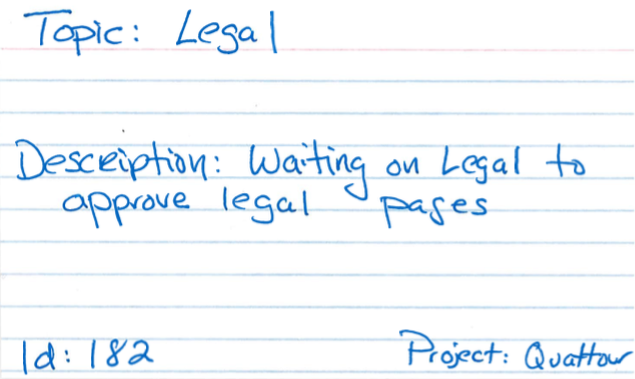
\includegraphics[width=3in]{waste_images/retro_index_card.png}}
\caption{Example Retro Topic Index Card}
\label{exampleRetroTopicl}
\end{figure}

 When \textit{removing waste} appeared as a core category, we analyzed data from retrospectives to investigate (theoretical sampling). After removing irrelevant topics (e.g. complaints about the weather), we printed each retro item onto an index card with its original retro topic, enhanced description, ID, and team name (see Figure \ref{exampleRetroTopicl}).

Two researchers with first-hand experience of the projects coded the retro topics and merged duplicate topics. We iteratively reorganized categories, keeping similar items together and dissimilar items apart. Figure \ref{ChainOfEvidence} gives an example classification for the \textit{psychological distress} waste. The figure shows the waste category, its cause categories and properties, and examples of observed retrospective topics illustrating the waste.  Appendix \ref{AppendixChainOfEvidence} presents the entire chain of evidence for all waste categories.

We often stopped to record new insights. When the categories began to stabilize, we compared each category against the other categories looking for relationships. Once we felt that the categories were stable, we performed a final review of each category to verify that the cards belonged to it.

We continued theoretical sampling for team code ownership and removing waste in additional interviews and participant observations until no further categories were evident, i.e. theoretical saturation. 

In summary, the data advanced from the initial codes to focused codes, focused codes to core categories, and core categories to an emergent theory. 



\chapter{Constructing Products: Sustainable Software Development}
\label{SustainableSoftwareDevelopmentChapter}

\section{Summary}

\textit{Context:} This chapter examines how software development teams build a product once  user centered design determines and validates the features and product prioritizes the stories into a backlog.

\textit{Objective:} The purpose was to understand how to develop software effectively, even in the face of team disruption. Conventional wisdom says that team disruptions (like team churn) should be avoided. We coined the phrase \quotes{Sustainable Software Development} to describe the principles, policies, and and practices because the observed software development projects succeeded despite high disruption. 

\textit{Method:} Following Constructivist Grounded Theory, we conducted participant-observation of several projects at Pivotal (a software development company), and interviewed many software engineers, interaction designers, and product managers. 

\textit{Results:} This chapter introduces a descriptive theory of Sustainable Software Development. The theory encompasses principles, policies, and practices aiming at removing knowledge silos and improving code quality (including discoverability and readability), hence leading to development sustainability. 

\textit{Limitations:} While the results are highly relevant to the observed projects at Pivotal, the outcomes may not be transferable to other software development organizations with different software development cultures.

\textit{Conclusion:} The theory refines and extends the understanding of Extreme Programming by adding new principles, policies, and practices (including Overlapping Pair Rotation) and aligning them with the business goal of sustainability. 

\section{Introduction}
Imagine being a software development manager when one of your top engineers, Dakota, gives notice and is moving on to a new job opportunity. You are simultaneously excited because the new position provides a great career opportunity for someone you respect, yet distressed that her departure may exacerbate your own project. How will the team overcome this disruption? Your investment in this engineer and her entire accumulated knowledge about the project is evaporating. Dakota developed some of the systems' trickiest, most important components. How long will it take the other programmers to assimilate Dakota's code?  How will this affect their productivity and future development?


Conventional wisdom says that team churn is detrimental to project success and that extensive documentation is needed to mitigate this effect. Unfortunately, documentation quickly becomes out-of-date and unreliable \cite{Lethbridge2003Documentation}, undermining this approach. During a Grounded Theory study, we observed projects succeed despite high disruption and little documentation. This raised the following research question: \quotes{How do the observed teams develop software effectively while overcoming team disruption?}

Exploring this question resulted in a descriptive theory of \quotes{Sustainable Software Development.} The theory explains how a collection of synergistic principles, policies, and practices help develop software effectively while overcoming team disruption. This is done by engendering a positive attitude towards team disruption, encouraging knowledge sharing and continuity, as well as prioritizing high code quality. Here, \textit{team disruption} refers to substantial ongoing changes in team composition, including team members joining or leaving, as well as temporary vacations or leave of absence. 

Section \ref{SustainableSoftwareDevelopmentRelatedWork} describes related work on Extreme Programming and team disruption. Section \ref{SustainableSoftwareDevelopmentResearchMethod}, reviews the research method to derive a descriptive theory supported by empirical data. Section \ref{SustainableSoftwareDevelopmentResearchMethod} also presents the research context, introducing both the company and one of the \numberOfObservedProjects{} projects under study. Section \ref{Theory} describes the theory and how its principles, policies, and practices work together to achieve software development sustainability. Section \ref{TheoryEvaluation} evaluates the theory using established criteria for evaluating a Grounded Theory. The last sections of the chapter examine threats to research validity and summarize the research.
\section{Related Work}
\label{SustainableSoftwareDevelopmentRelatedWork}
In Extreme Programming \cite{BeckExtremeProgramming2004}, Kent Beck describes a set of interdependent practices that manage feature development (much like Scrum \cite{SchwaberScrum}), as well as technical practices that facilitate a collaborative team environment. Extreme Programming comprises 13 primary practices and 11 corollary practices. 

One Extreme Programming practice, collective ownership, simply means that \quotes{anyone on the team can improve any part of the system at any time.} Beck contrasts collective ownership with \quotes{no ownership} and \quotes{individual ownership.} With collective ownership, every developer takes responsibility for the whole of the system. When developers see opportunities to improve the code, they go ahead and improve it if it makes their life easier \cite{BeckExtremeProgramming2000}. Later, \quotes{collective ownership} was renamed to \quotes{shared code} \cite{BeckExtremeProgramming2004}. 

One Extreme Programming practice contributing to collective code ownership is pair programming. Pair programming is where production code is created by two developers working together at a single computer \cite{BeckExtremeProgramming2004}. Extreme Programming does not prescribe how pairs are formed or for how long a pair works together. Williams presents a pair rotation strategy for maintaining specialization, by \quotes{choosing the right partner for the right situation}  \cite{Williams2002}. People are assigned modules of the code to own based upon expertise and find partners from neighboring modules. While knowledge is shared with pairing, one person owns every story that touches their part of the system, building individual code ownership. In one case study, the project started with a pair rotation strategy based on skillsets but evolved into a daily rotation determined randomly \cite{Vanhanen2007}. Some teams use a pair programing matrix \cite{AlaverdyanPairProgrammingMatrix} (also called a pairing ladder \cite{Davies2009AgileCoaching}) to track who has paired with whom for the purpose of pairing people who have not paired recently.

Truck Number is \quotes{The size of the smallest set of people in a project such that, if all of them got hit by a truck, the project would be in trouble.} \cite{WikiTruckNumber}. Truck Number, or Bus Count, reminds management about the effects of disruptive events for a team. In 1994, Coplien \cite{Coplien1994} mentions \quotes{Truck Number} as a risk to his Solo Virtuoso pattern of using only one talented developer to create a software system. Awati suggests that Truck Number can be increased by reducing complexity, cross-training, and documentation \cite{AwatiBusFactor}, all of which are found in Extreme Programming. However, Extreme Programming implements \quotes{documentation} as discoverable, intention revealing code. Ricca \cite{Ricca2011TruckFactor} examines the difficulty in computing the Truck Number. 

Rigby quantifies turnover using knowledge at risk analysis on abandoned files  \cite{Rigby2016Turnover}. A line of code is abandoned if the most recent contributor has left the company.  A file is abandoned if more than 90\% of the lines in the file are abandoned.  Izquierdo examines how teams managed orphaned code \cite{Izquierdo2009Turnover}. Joseph examines job turnovers to understand the reasons developers leave their company  \cite{Joseph2007Turnover}.  

\section{Research Method}
\label{SustainableSoftwareDevelopmentResearchMethod}
\subsection{Constructivist Grounded Theory}

% When deciding which version of Grounded Theory to employ, we selected Constructivist Grounded Theory \cite{Charmaz} because it allows for the recording and transcription of interviews, enables literature review when appropriate in the research process, and builds upon decades of grounded theory research and experience.

% The philosophical stance of constructivism (as opposed to positivism) acknowledges the reseacher's and participants' contribution in the construction of concepts. 
% While there are absolute facts to be obtained in fields such as mathematics and the sciences, understanding people is a messy, organic process. For software engineering research, Constructivist Grounded Theory seems aptly suited since software development is a socio-technical endeavor.

% As described in Chapter \ref{ConstructivistGroundedTheory}, Constructivist Grounded Theory provides an iterative approach to data collection, data coding, and analysis resulting in an emergent theory. When starting a Grounded Theory research study, the core question is, \quotes{What is happening here?} \cite{GlaserTheoreticalSensitivity}. The initial core question was \quotes{What is happening at Pivotal when it comes to software development?}

% For this grounded theory study, the two primary data sources were field notes collected during continuous participant observations of a seven-month project and interviews with Pivotal software engineers, interaction designers, and product managers. Interviews were recorded, transcribed, coded, and analyzed using constant comparison. In addition, participant-observation was used for \numberOfObservedProjects{} projects.

% \subsection{Participants}
% The interviewees consisted of 21 interaction designers, product managers, and software engineers who had experience with Pivotal's software development process. They were distributed across four different Pivotal offices. Interaction designers identify user needs predominately through user interviews; create and validate user experience with mockups; determine the visual design of a product; and support engineering during implementation. Product managers are responsible for identifying and prioritizing features, converting features into stories, prioritizing stories in a backlog, and communicating the stories to the engineers. Software engineers implement the solution. Participants were not paid for their time. 
% \subsection{Data Collection}
% The initial interviews were open-ended explorations starting with the question, \quotes{Please draw on this sheet of paper your view of Pivotal's software development process.} The interviewer specifically did not force initial topics and merely followed the path of the interviewee. 

% While exploring new emergent core categories, whenever possible, subsequent interviews were initiated with open-ended questions.  For example, asking the participant, \quotes{Please draw your feelings about the code} often resulted in conversations about code ownership. 

% In addition to collecting data from interviews, field notes were collected while working as an engineer on the project described in Section \ref{ProjectQuattuor}. The field notes comprised multiple paragraph entries recorded several times a week, collected over seven months. These notes described individual and collective actions, captured what participants defined as interesting or problematic, and included anecdotes and observations. 
% \subsection{Data Analysis}
% Data analysis began with line-by-line coding as recommended by Charmaz \cite{Charmaz}. Coding line-by-line helps the researcher identify nuanced interactions in the data and avoid jumping to conclusions. The data then advanced from these initial codes to focused codes, focused codes to core categories, and core categories to an emergent theory. 

% The initial codes were reviewed while reading the transcripts and listening to the audio recordings. During weekly research collaboration meetings, the coding process was discussed. To avoid missing insights from these discussions \cite{GlaserTheoreticalSensitivity}, these discussions were recorded and transcribed them into grounded theory memos. 

% As data was collected and coded, the initial codes were recorded in a spreadsheet. Constant comparison generated focused codes. Only ideas expressed by multiple interviewees informed focused codes and subsequent analysis. 

Constantly comparing new codes to existing codes refined the codes and eventually generated categories. Periodic audits checked each category for cohesion by comparing its codes. When this became complex, the codes were printed on index cards, and then arranged and re-arranged until cohesive categories emerged. Memos were written to capture the analysis of codes, examinations of theoretical plausibility, and insights. 
Constant comparison facilitated the identification of \quotes{the conceptual relationship between categories and their properties as they emerged} \cite{GlaserBasics}, leading to a resulting descriptive theory. The resulting theory is presented in Section \ref{Theory} and illustrated in Table \ref{SustainableSoftwareDevelopmentTable}. The table includes the main categories and their organization into principles, policies, and practices. Examples of quotes leading to some categories are presented in Table \ref{ChainOfEvidenceTable}.

\begin{table}[t]
\renewcommand{\arraystretch}{1.5}
\centering
\caption{Quotes for Selected Categories}
\label{ChainOfEvidenceTable}
\begin{tabular}{|p{\twoColumnWidth}|}
\hline
Engendering Positive Attitudes Toward Team Disruption \\
\hline
\participantQuote{I'm excited when a new person joins the team. That person has experience that might add something to the project.} \\

\participantQuote{I like that people bring new energy. Projects often get into the state of a lull with the same people working on it and have the same cadence. New people bring a new perspective. [Two engineers recently joined] and it was really cool to see their fresh perspective. I always like people joining a project.} \\

\participantQuote{Team members go out of their way to make new teammates feel welcome and help ramp them up.} \\

\hline
Team Code Ownership \\
\hline
\participantQuote{I feel ownership of the code as a whole, and I feel empowered and able to go and work on any part of the codebase.} \\
\participantQuote{I don't feel like I have [individual] ownership. It's really a collaborative effort to achieve where we are today \ldots I feel like everybody owns this product.} \\
\participantQuote{There is a lot of emphasis that you are not your code.} \\
\participantQuote{I never feel like a specific piece is mine or something belongs to other people.}\\

\hline
Overlapping Pair Rotation \\
\hline
\participantQuote{To make sure that knowledge silos don't form we rotate pairs. As people work on specific stories and specific parts of the code, we want to share that knowledge.} \\

\participantQuote{Rotating pairs reduces knowledge silos and reduces the bus factor. We do not want the departure of one developer from the project to cripple the project.} \\

\participantQuote{We rotate pairs because everyone has a different set of knowledge. When you work with someone you get a little bit of that knowledge. The more you pair with them, the more knowledge you get.} \\

\hline
\end{tabular}
\end{table}


% \subsection{Research Context}
% \label{SustainableSoftwareDevelopmentResearchContext}

% Pivotal is a large American software company (with 16 offices around the world), which provides solutions for cloud-based computing, big data, and agile development. 

% This study focuses on one Pivotal subsidiary, Pivotal Labs, which provides agile developers, product managers, and interaction designers to other firms. Its mission is to deliver highly-crafted software products and provide a transformative experience for clients' engineering cultures. To change the client's development process, Pivotal combines the client's software engineers with Pivotal's engineers at a Pivotal office where they can experience Extreme Programming in an environment conducive to agile development. For startups, Pivotal engineers might be the first to work on the project. For enterprise clients, Pivotal provides additional engineering resources to accomplish new business goals. 

% Pair programing ability is a strong pre-requisite for becoming a Pivotal Labs developer. During job interviews, applicants engage in multiple pair-programming rounds to reveal their ability to listen to and empathize with pairs. 

% Typical teams include six developers, one interaction designer, and a product manager. The largest project in the history of the Palo Alto office had 28 developers while the smallest had two. Larger projects are organized into smaller coordinating teams with one product manager per team and one or two interaction designers per team. 

% Commonly utilized technologies include Angular, Android, backbone, iOS, Java, Rails, React, and Spring. These are often deployed onto Pivotal's Cloud Foundry. 

% Pivotal Labs has followed Extreme Programming \cite{BeckExtremeProgramming2004} since the late 1990's. While each team autonomously decides what is best for each project, the company culture strongly suggests following all of the core practices of Extreme Programming, including pair programming, test-driven development, weekly retrospectives, daily stand-ups, a prioritized backlog, and team code ownership.

% Only teams at Pivotal Labs were observed. Other teams, especially teams in other divisions, might have a different culture and follow different software practices.

\subsection{Project Context: Project Quattuor}
\label{ProjectQuattuor}
While \numberOfObservedProjects{} projects were observed in total, this discussion focuses on Project Quattuor. This project shares many similarities with the other projects. To preserve client confidentiality, this study describes Project Quattuor's project as a mobile application for controlling expensive equipment.

The project lasted 43 weeks. The initial four weeks, called Discovery and Framing, include four main activities: 1) interaction designers investigate user needs through user interviews, 2) product managers define the features for the initial release based on those needs, 3) interaction designers create an initial interaction design and validate their mock-ups with users, and 4) engineers mitigate technology risks. Discovery and Framing was followed by code implementation, resulting in two releases to both the Apple store and Google Play store.

\begin{figure}[t]
\centering
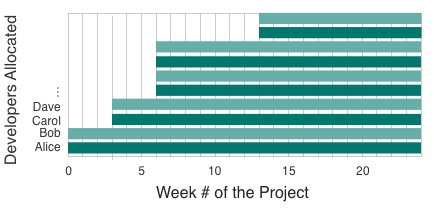
\includegraphics[width=\twoColumnWidth{}]{sustainable_software_development_images/OriginalDeveloperStaffingV3.jpg}
\caption{Planned Developer Staffing}
\label{PlannedDeveloperStaffing}
\end{figure}

The 35-person project consisted of an iOS team of ten engineers, an android team of ten engineers, and a Java back-end team of eight engineers with the support of two to four interaction designers and three product managers. Here the discussion will focus on the iOS team. The first iOS release to the Apple store occurred in week 23. Given the success of the project, the client extended the engagement for a second iOS release that happened on week 43. 

Figure \ref{PlannedDeveloperStaffing} shows the staffing plan at the start of Project Quattuor. The plan was to start the project with two developers, while adding more developers as more tracks of work became available. The plan is consistent with the observed projects with a gradual ramping up of developers to a stable team. Figure \ref{DeveloperStaffing} shows the actual staffing, which is quite different from the plan.

The bar chart on the top of Figure \ref{DeveloperStaffing} shows when individual developers started and stopped working on the project. Five developers were on the project for most of its duration, while 22 people worked on the project in total. The maximum team size was 12 developers working together at the same time. Five engineers worked for 70\% or more of the project's duration. The graph on the bottom of Figure \ref{DeveloperStaffing} shows the total number of developers allocated to the project at any given week. Developers ramped up from week 5 to week 12, with an average team size of 10 and a maximum of 12 developers.

Developers were routinely rotated and were replaced for various reasons, including promotions, medical leave, leaving the company, transferring to a different office, and vacations. Atypically, the client was more concerned with feature development than cost, so absent developers were replaced, leading to 22 different people working on the same ten-person project. 

The ongoing rotation of team members likely undermined the team's sense of identity \cite{TuckmanModel}. In addition, the project experienced many challenges, including not having access to production back-end systems or expensive dependent physical components, and cultural differences between Pivotal and the client's deployment organization. Yet the team successfully completed the project. The client was delighted, even claiming that the team delivered a multi-year project in five months when the team delivered the first release. 

Contrary to conventional wisdom, high team disruption did not appear to negatively influence the success of Project Quattuor. This observation raises the research question: \quotes{How do the observed teams develop software effectively while overcoming team disruption?}


%\begin{figure*}[t]
%\centering
%\includegraphics[width=\twoColumnWidth{}]{DeveloperStaffingV4.jpg}
%\caption{Actual Developer Staffing}
%\label{DeveloperStaffing}
%\end{figure*}

\begin{figure}[t]
\centering
\includegraphics[width=\twoColumnWidth{}]{sustainable_software_development_images/DeveloperStaffingV4.jpg}
\caption{Actual Developer Staffing}
\label{DeveloperStaffing}
\end{figure}

\begin{table*}[t]
\renewcommand{\arraystretch}{1.5}
\centering
\caption{Theory of Sustainable Software Development: Principles, Policies, and Practices}
\label{SustainableSoftwareDevelopmentTable}
\begin{tabular}{|p{2.5in}|p{3.5in}|}
\hline
\multicolumn{2}{|c|}{Sustainable Software Development}              
\\
\hline
Underlying Principles & Engendering a Positive Attitude Toward Team Disruption \newline Encouraging Knowledge Sharing and Continuity \newline Caring about Code Quality \\ 
\hline
Policies & Team Code Ownership \newline Shared Schedule \newline Avoid Technical Debt  \\
\hline
Removing Knowledge Silos Practices & Continuous Pair Programming \newline Overlapping Pair Rotation \newline  Knowledge Pollination  \\
\hline
Caretaking the Code Practices & TDD / BDD \newline Continuous Refactoring  \newline Supported by Live on Master \\
\hline
\end{tabular}
\end{table*}


\section{Theory of Sustainable Software Development}
\label{Theory}

Sustainable software development refers to the ability and propensity of a software development team to mitigate the negative effects of major disruptions, especially team churn, on its productivity and effectiveness. The theory of Sustainable Software Development, summarized in Table \ref{SustainableSoftwareDevelopmentTable}, is targeted towards software developers and has emerged from the Grounded Theory research described above. We hypothesize that sustainability emerges from synergistic principles, policies, and practices, which collectively explain how the observed Pivotal teams overcome disruption. The ability of any pair to work on any story while caring about the code is the primary mechanism by which these principles, policies, and practices mitigate disruption. 

This section documents each principle, policy, and practice. For each policy and practice, the sub-section presents how it is used at Pivotal, and discuss anti-patterns and potential alternatives. Deeper descriptions are provided for practices rarely documented in the literature.
\subsection{Principles}

\subsubsection{Engendering Positive Attitudes Toward Disruption}
Conventional wisdom says that team disruption should be avoided. Yet, team disruption is a reality in the industry, as exemplified by Project Quattuor where only five of 22 developers worked on the project for most of its duration (see Figure \ref{DeveloperStaffing}). However, the observed organization engendered a positive attitude towards disruption, transforming a challenge into an opportunity and hence demonstrating remarkable business agility. Team members rolling off the project were replaced as needed. New members rolling onto the project were viewed as an opportunity to improve the current code base by providing a fresh perspective. When a new team member did not understand the code base, he or she revealed issues with code discoverability. New team members often questioned the team's assumptions and challenged \quotes{cargo culting.} 

The first underlying principle of Sustainable Software Development is engendering an open and positive attitudes towards team disruption, transforming a challenge into an opportunity to improve code quality.

\subsubsection{Encouraging Knowledge Sharing and Continuity}
Despite the fresh perspectives added by new team members, team disruption can precipitate in significant knowledge loss for the organization. Policies and practices that encourage knowledge sharing and continuity mitigate this risk. These policies are Team Code Ownership, and Shared Schedule, while the practices are Continuous Pair Programming, Overlapping Pair Rotation, and Knowledge Pollination (which are discussed below).

The second underlying principle of Sustainable Software Development is encouraging knowledge sharing and continuity, enabling the knowledge to spread from one developer to the next, and eventually reach the entire team. Knowledge sharing and continuity make the team more resistant to disruption. 

\subsubsection{Caring about Code Quality}

Enabling knowledge sharing and continuity does not guarantee sustainable development if the team starts incurring technical debt \cite{McConnellTechnicalDebt}. A set of policy and practices aimed at taking good care of the code itself mitigates this risk. The policy is Avoid Technical Debt, while the practices are Test-Driven Development / Behavior-Driven Development and Continuous Refactoring (which are discussed below).

The third underlying principle of Sustainable Software Development is caring about code quality, hence avoiding technical debt and enabling sustainable team productivity.
\subsection{Policies}

\subsubsection{Team Code Ownership}

\textbf{Description:} Team code ownership is the extent to which any team member can modify any part of the team's code. Code ownership is influenced not only by official policy but also each developer's familiarity with and emotional relationship to the code.

\textbf{Purpose:} Everyone on the team is responsible for the team's code. Simply saying \quotes{Any team member can modify any piece of the code} is not sufficient to achieve the desired result of team code ownership. We documented five factors that affect the team's sense of code ownership and eight risks observed on Pivotal teams \cite{SedanoTeamCodeOwnership}. Achieving team code ownership requires a set of enabling practices. These enabling practices aim at removing knowledge silos and taking good care of the code, as described in the following sections.

\textbf{At Pivotal:} Every developer is empowered to work on any part of the team's code and is encouraged to refactor any code section to improve its quality as needed, especially in cases of low code discoverability and readability.

\textbf{Anti-pattern:} Removing team code ownership makes sustainable software development challenging. Every line of code written via strong ownership might create a knowledge silo. Code reviews are a mitigation strategy with an asynchronous delay. When the delay is too long, merging code onto the master becomes problematic, which discourages Continuous Refactoring. 

\subsubsection{Shared Schedule}
\textbf{Description:} Shared Schedule signifies that all team members have the same work schedule. 

\textbf{Purpose:} Shared Schedule enables Continuous Pair Programming, Overlapping Pair Rotation, and Knowledge Pollination practices. With Shared Schedule, teams form new pairs at the beginning of the day. The evening becomes a natural interruption to the continuous software development workflow. 

\textbf{At Pivotal:} Team members at the Palo Alto office work Monday to Friday from 9:00 am to 6:00 pm. This is done without management coercion; each team member agreed to this fixed schedule to achieve the benefits of Sustainable Software Development. While Shared Schedule is the norm, exceptions are possible. 

Pivotal prefers co-located teams in order to promote synchronous and osmotic communication. Project Quattuor was an exception with the team split between Palo Alto and San Francisco. Each day, developers in one location remotely paired with developers in the other location to spread the knowledge across the two offices.

\textbf{Anti-pattern:} Flexible work hours potentially jeopardizes Continuous Pair Programming, Overlapping Pair Rotation, and Knowledge Pollination practices. A team with flexible work hours might find it difficult to pair program on all stories (as described in the Continuous Pair Programming practice). A team member consistently soloing from 8:00 am to 10:00 am might be building knowledge silos. 

When developers arrive whenever they feel like it, rotating pairs (as described under the Overlapping Pair Rotation practice) becomes awkward, as there is no longer a natural time to rotate pairs. Trying to schedule a time midday to rotate pairs feels artificial. Even if the team says they will rotate later in the day, once pairs get into their stories and form context on what needs to be done, they typically forget about re-pairing until it is time to go home.

Pivotal experimented with pairing when developers arrived, but this meant that developers coming early were making decisions for the team members who arrived later, hence loosing some benefits of pair programming. 

\textbf{Alternatives:} A possible mitigation strategy could be to adopt core work hours. Individuals would solo on simple cleanup chores outside of core hours, and switch to pair programming for feature development when the whole team is in the office. 

\subsubsection{Avoid Technical Debt}
\textbf{Description:} Technical Debt refers to delaying needed technical work, by taking technical shortcuts, usually in pursuit of calendar-driven software schedules \cite{McConnellTechnicalDebt}. 

\textbf{Purpose:} Avoid Technical Debt enables a team to balance feature development with Continuous Refactoring (as described under the Continuous Refactoring practice). When a team is pressured to finish work by a deadline, they might be tempted to focus on feature delivery, take on technical debt, and stop refactoring. When a team delays refactoring and takes on technical debt, the code becomes harder to work with, which in turn makes it more difficult for developers to rotate onto that part of the code base. There is a dialectic tension \cite{RalphProcessTheories} between Continuous Refactoring and delivering more features while accruing technical debt.

\textbf{At Pivotal:} A pair tends to create well-crafted code by avoiding shortcuts and short-term fixes. The team codes for the \quotes{present} by building the simplest solution for the current story. The team eschews over-engineering for potential future features. The team avoids technical debt by building the best solution for the moment at hand. When inheriting a large code base with existing technical debt, one observed team choose to actively paying down technical debt while delivering new features. 

\textbf{Anti-pattern:} On Project Quattuor, the product manager suggested that the team deliver more stories at the cost of technical debt to make a release date. Some team members followed this suggestion, skipped the refactoring step, and introduced harder to maintain code. This decision made it difficult for pairs to rotate onto parts of the code. Pairs making the decision to skip refactoring caused future pain for the next pair to work with that part of the code. Immediately after the first release, the team spent several weeks refactoring the code to pay down the debt and consistently deliver new features again.
\subsection{Removing Knowledge Silos Practices}
This section presents practices for encouraging knowledge sharing and continuity, enabling the knowledge to spread from one developer to the next, and eventually reach the entire team. This phenomenon is illustrated in Figure \ref{KnowledgeSharing}, where letters A to F represent six developers working in pairs.

\begin{figure}[t]
\centering
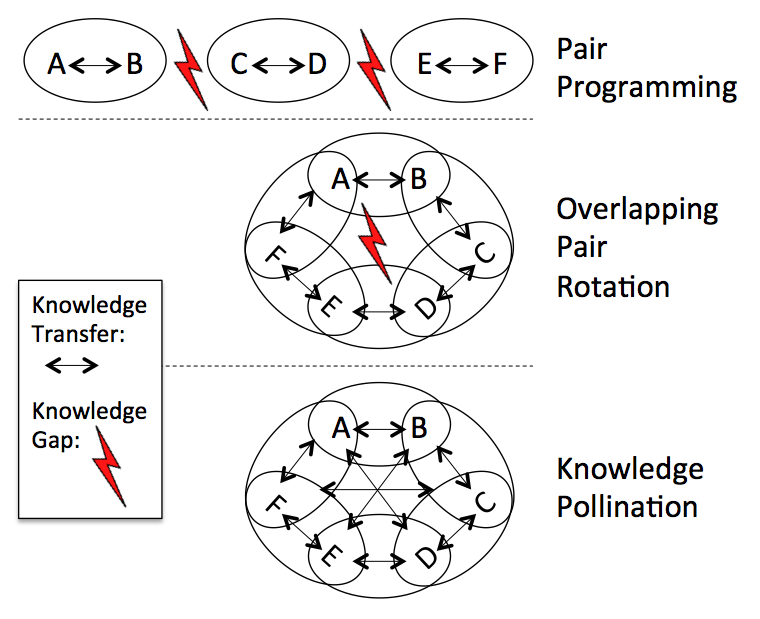
\includegraphics[width=\oneColumnWidth{}]{sustainable_software_development_images/KnowledgeSharingLevels.png}
\caption{Three Levels of Knowledge Sharing}
\label{KnowledgeSharing}
\end{figure}

\subsubsection{Continuous Pair Programming}
\textbf{Description:} Continuous Pair Programming is two developers collaborating to write software together as their normal mode of software development.

\textbf{Purpose:} When two developers work together, they are likely to bring more knowledge, and generate more diverse solutions compared to a solo developer. Additionally, there are many documented benefits of pair programming \cite {Williams2002}. When two developers work together, knowledge spreads from one developer to the next \cite{Zieris2016KnowledgeTransfer}, as illustrated in Figure \ref{KnowledgeSharing}. Overall, pairing reduces knowledge silos and can improve code quality.

\textbf{At Pivotal:} Pairing happens with two monitors, two keyboards, two mice, and one computer. Developers always work in pairs, unless exceptional circumstances arise. For instance, solo programming occurs when one developer is out of the office for part of the day (e.g. at the doctor's office), out of the office the whole day (e.g. out sick), or involved in another business activity for a few hours (e.g. interviewing candidates, scoping a new project). When solo programming, developers take low-risk chores, refactorings, or stories. With any sizable project, there usually is something the team has been meaning to do that one person can safely do and report back to the team on its completion. 

\textbf{Anti-pattern:} Removing this practice results in solo programming where there is a clear owner for the code written. This would increase individual ownership and start creating knowledge silos. 

\textbf{Alternatives:} In solo programming, to remove silos, developers could take the stories for the part of the code they know least about. Assigning stories to developers who have the least understanding of the code could be a hard sell to management as it reduces productivity (at least initially). Bird \cite{BirdDontTouchMyCode} suggests that this approach would introduce more defects. 

\subsubsection{Overlapping Pair Rotation}
\label{OverlappingPairRotationSection}
\textbf{Description:} Overlapping Pair Rotation happens when there is a rotation of the people working on a track of work: one developer rolls off the track and another developer rolls on, keeping continuity of one developer at each rotation. This results in knowledge continuity for a track of work, as illustrated in Figure \ref{KnowledgeSharing}. Typically, rotations happen in the morning as the evenings provide a natural interruption to the work. 

\textbf{Purpose:} The rotation of developers helps spread knowledge and promotes team code ownership. The goal is to prevent the situation where one or two developers understands how  part of the system works and must be assigned any story related to that part of the system. The entire team should be able to modify the code. Rotation helps prevent knowledge silos and individual code ownership from forming. 

\textbf{At Pivotal:} Whenever a knowledge silo begins to emerge, the team actively fights against it and tries to spread that knowledge around through pair rotation. During the study, three strategies were observed.

\textit{Optimizing for people rotation:} Most teams rotate based on who has paired with whom. Developers try to pair with the person they \quotes{least recently paired with} (basically a Least Recently Used strategy). Some teams use rotation techniques or tools to track this information.

This strategy does not clearly articulate the purpose of knowledge silo removal and the need for knowledge transfer. As an example, developers who recently left a track of work might ask to be rotated back without realizing the potential cost to the team. This prevents an opportunity to spread the knowledge to the rest of the team. (This issue is more serious on larger teams; on a four person team, this is not an issue).

\textit{Optimizing for personal preferences:} A few teams allow developers to pick with whom they will work or on which stories to work based on individual preferences. This has the same downsides as the previous strategy. 

\textit{Optimizing for context sharing:} A few teams are experimenting with rotating onto a track the person who has not been working on the track for the longest time. The goal each day is for the developer leaving the track next to empower the developer who will remain on the track. Before any rotation, the remaining developer is asked, \quotes{Was enough context shared with you?} If the answer is no, then the first developer does not leave and the pair continues to work together for another day. This provides a feedback loop on how well the team is transferring knowledge. 

\textbf{Anti-pattern:} Removing this practice means that developers can work on the same part of the code base for extended periods of time, developing individual code ownership and knowledge silos. One participant described their experience at a previous company that follows Extreme Programming. Developers could be paired for more than a month working on only one part of the system. This lack of pair rotation led to deep knowledge silos. 

Ideally, developers work on the next, non-blocked story at the top of the backlog. When developers start skipping down the backlog, it can be an indication that they might not have enough context to work on any story. On Project Quattuor, a knowledge silo emerged around a complicated bug related to an obsolete technology that only a handful of people understood. Often developers would skip over stories and bugs related to that technology. At one point, the product manager reminded the team to keep \quotes{working from the top of backlog.}

Sometimes a developer wants to see a story through to completion over multiple days. Maybe he or she enjoys the technology or the feature. In these situations, agreeing to the request may result in forming knowledge silos and creating a sense of personal ownership. Statements like \quotes{we need Marion on that story, only she really knows the Apple watch code base,} or \quotes{shea knows the ins-and-outs of the legacy integration, we need him to work on this story,} suggest that knowledge silos have emerged. 

\textbf{Alternatives:} Team members that build a knowledge silo can share what they learned through a demo, code walk through, or a team huddle. This helps a team share knowledge, but is less effective than working directly with the code. 

\subsubsection{Knowledge Pollination}
\textbf{Description:} Knowledge Pollination refers to the set of activities contributing to knowledge sharing in an unstructured way. Examples include daily stand-up meetings, weekly retrospections, writing or sketching on whiteboards, overhearing a conversation, using the backlog to communicate current status about a story, calling out an update to the entire team, or simply reaching out to others to ask questions as needed. 

\textbf{Purpose:} Knowledge Pollination contributes to spreading knowledge among the team as illustrated in Figure \ref{KnowledgeSharing}.

\textbf{At Pivotal:} Daily standups create awareness of who is working on what. Teams can write down a \quotes{parking lot} of issues to discuss during daily standups. A pair may record the current status of a blocked story so that the next pair picking it up knows the situation. Osmotic communication helps when a developer overhears another pair discussing an issue and offers needed knowledge. Instead of thrashing, a pair interrupts another pair to gain the needed information. Thus, interruptions are encouraged because they make the entire team more efficient as knowledge pollinates across the team. 

Calling out an update to the entire team might be a simple as shouting \quotes{the build is broken, we are looking into it}, or this interchange: \quotes{we just checked in a presenter,} followed by \quotes{we just used your presenter. That's great collaboration.}

While working on a story, a pair may discover that they are missing some key context that prevents them from efficiently proceeding. If the issue is about the acceptance criteria for a story, they clarify with the product manager. If the issue is about the code base, the pair can ask the people who recently worked on that section of code, or ask the entire team. To determine whom to ask, the pair may remember who did what at stand-up, look through Pivotal Tracker (an agile project management tool) to see who worked on a story, or check out source code version history (e.g. git annotate). Two-, four-, and six- person teams seem to have collective memory of who worked on which features from the daily stand-ups. 

These mechanisms help a team build awareness. Chong observed that \quotes{transmission of awareness information is a relatively effortless act in the XP environment} in her ethnographic study comparing an Extreme Programming team to a traditional team \cite{ChongNominum}.
 
\textbf{Anti-pattern:} An organization that provides little opportunity to share knowledge leads to wasted time as developers must acquire the knowledge through other means or end up reinventing the wheel.
\subsection{Caretaking the Code Practices}
\subsubsection{Test-Driven Development, Behavior-Driven Development}
\textbf{Description:} In Test-Driven Development (TDD) developers write unit tests before creating a design and writing code. In Behavior-Driven Development (BDD) developers implement acceptance tests before creating a design and writing code. Most lines of production code are tested before the production code is written. The software's design emerges from the tests and subsequent refactorings.

In Extreme Programming, Kent Beck describes his corresponding \quotes{Testing} practice as developers writing \quotes{automated unit tests} and implementing customer provided \quotes{functional tests} for story acceptance \cite{BeckExtremeProgramming2000}. Later, he refines these ideas as \quotes{Test-first programming} \cite{BeckExtremeProgramming2004}. 

\textbf{Purpose:} This practice creates a safety net and empowers a pair to have the confidence to modify the code base. This enables any pair to pick up any story. Continuous Refactoring results in easier to modify tests.

\textbf{At Pivotal:} Developers use a combination of TDD and BDD. While each project is different, programmers tend to use BDD to describe interactions between the user and the system and TDD at a unit test level. Teams use a variety of TDD strategies including testing the responsibilities and interactions \cite{Goose} or contract testing using mocks \cite{RainsbergerIntegrationTestsYouTube}. In Pivotal's ideal, the design emerges from the creation and exploration of the test cases. 

\textbf{Anti-pattern:} Without this testing practice, developers no longer have the confidence to change any part of the code as they may unknowingly end-up breaking something else. 

\textbf{Alternatives:} For a system without a test suite documenting the system specification, a possible remedy is for developers to own particular parts of the system in order to understand the ramifications of changes. Creating strong code ownership and knowledge silos is exactly the problem that sustainable software development is trying to solve.

Writing tests after the code is written could produce a safety net for refactoring, provided that tests correctly exercise the system. (A test that never failed might not be testing anything). We did not observe this behavior and future research is necessary to determine if any testing approach is sufficient for sustainable software development.

\subsubsection{Continuous Refactoring}
\textbf{Description:} Continuous Refactoring is the systematic improvement of the code base concurrently with new feature development. When developers identify something wrong such as a code smell, they simply fix it. In this regard, developers are caretaking the code by continuously improving it. This practice results in an emergent software design, as well as empathy for the code as developers learn to \quotes{listen to the code.} 

%Continuous Refactoring is one way to prevent technical debt from accumulating. When a team employs continuous refactoring, the team refines a code base towards simple design, intention revealing code, and discoverable code. 

\textbf{Purpose:} Continuous Refactoring enables any pair to work on any part of the system. Long-term benefits for the team include increased code discoverability, code readability, code modifiability, and code simplicity. 

\textbf{At Pivotal:} Developers typically do some refactoring while implementing stories. Developers are encouraged to improve the code's design, make the code easier to understand, and increase the discoverability of a component based on its responsibility. Usually, the team prefers \quotes{pre-factoring} where the developer does the complicated work to make the implementation of the current story as simple and easy as possible, as opposed to \quotes{post-factoring} where refactoring happens after the story is done, but before it is delivered. 

\textbf{Anti-pattern:} Removing this practice might produce difficult to modify and messy code. Developers might not be able to easily work on any part of the code base. When refactoring is skipped, code might be simply bolted on to the existing design. Soon it becomes increasingly difficult to bolt more code on. A dilemma arises for the programmers working on the next story: do they continue bolting on more code, or do they perform the pretermitted refactorings? Removing this practice may also result in hard-to-change tests.

\textbf{Alternatives:} Postponing refactoring may be necessary in extreme situations, for instance, when the company might go out of business unless the company releases the next version. In such situations, the team risks taking on uncontrolled technical debt as \quotes{refactoring later} turns into \quotes{refactoring never.} 

\subsubsection{Live on Master}
\textbf{Description:} Live on master means that developers integrate their code several times a day, as quickly as possible. ExtremeProgramming.org calls this practice \quotes{Integrate Often} \cite{WellsIntegrateOften}.

\textbf{Purpose:} For teams to continuously refactor and minimize the waste of merge conflicts, the entire team needs to routinely merge their code onto master. If a pair communicates to the team that they are actively \quotes{refactoring} a component, they are asserting exclusive temporary ownership over the file to avoid merge conflicts. While this is a normal practice for a few hours, if it happens for multiple days, the team is losing collective ownership of that code. The team is not able to receive any of the benefits until the work is merged back to master. 

\textbf{At Pivotal:} In the ideal workflow, developers merge their code to master many times a day. If a pair has not merged to master by the afternoon, the pair typically starts examining why this is difficult and explores ways of incrementally making changes. Developers may use branches to save spikes. When rotating pairs, developers may use branches to move work-in-progress code between machines. 

\textbf{Anti-pattern:} Removing this practice means that code lives in branches for days or weeks. Integrations might be painful due to merge conflicts and developers might delay needed refactorings. If a developer has code only on their machine, then no one else on the team can use or modify that code. When code lives only on one machine for many days in a row, the machine acts as a \quotes{virtual branch.} Running a Continuous Integration box and having long running branches is an anti-pattern.
\section{Theory Evaluation}
\label{TheoryEvaluation}

Charmaz identifies four criteria for evaluating a Grounded Theory: credibility (\quotes{Is there sufficient data to merit claims?}), originality (\quotes{Do the categories offer new insights?}), resonance (\quotes{Does the theory make sense to participants?}), and usefulness (\quotes{Does the theory offer useful interpretations?}) \cite{StolGroundedTheory}. 

\textbf{Credibility:} The current data set is rich and its analysis leads to theory saturation. (Saturation means that the properties of the theory are complete and are not affected by new data.) The data set comprises \numberOfInterviews{} intensive interviews conducted in four different offices, field notes from participant observation on Project Quattuor, and the use of participant-observation on \numberOfObservedProjects{} projects.

\textbf{Originality:} The theory uniquely depicts the principles, policies, and practices enabling software development sustainability in an organization. Since the organization under study follows Extreme Programming, it is not surprising that many of the practices of Sustainable Software Development are defined in Extreme Programming. However, overlapping pair rotation and its supporting principles, policies, and practices are central and unique to the proposed theory.

\textbf{Resonance:} The participants examined the theory. The theory resonates with their experience and reflects the way they work.

\textbf{Usefulness:} The theory informs Pivotal engineers as to why Pivotal purposefully avoids knowledge silos, and how the theory's principles, policies, and practices work together to accomplish the team's goals. The theory explains why the principles, policies, and practices should be incorporated together. A few managers use  the theory to help potential clients understand how Pivotal achieves the business goals of both the client and Pivotal.

\section{Threats to Validity}

\subsection{External Validity}

\textbf{Generalizability across situations:} Grounded Theory does not support statistical generalization from a sample to a population. The results may not be applicable to other teams or other domains. There are four broad types of scientific generalization: 1) from data to descriptions, 2) from descriptions to concepts, 3) from concepts to theory, 4) from theory to description \cite{Lee2003generalizing}. Grounded Theory research involves the first three kinds of generalization. Generalizing from a theory tested in one context to descriptions of a new context (the fourth kind of generalization) could be done by the researchers in the new context, on a case-by-case basis. However, we have not attempted to perform any type four generalizations at this time.

\subsection{Internal Validity}
\textbf{Researcher bias:} A risk of the participant-observer technique is that the researcher may lose perspective and become biased by being a member of the team. An outside observer might see something the researcher missed. This risk was mitigated by recording interviews and having another researcher review the results of the coding process.

\textbf{Prior knowledge bias:} With Grounded Theory, prior knowledge can aid the researcher in looking at interesting research questions or create difficulties by blinding the researcher about possible explanations \cite{GlaserIssues}. This risk was mitigated with another researcher reviewing the coding process. 

\section{Conclusions}
This research introduces a descriptive theory of \quotes{Sustainable Software Development} as a solution to the challenge of software development sustainability for an ever changing workforce. The theory emerged from a Constructivist Grounded Theory research study. By collecting data from \numberOfInterviews{} intensive interviews conducted in four different Pivotal offices, field notes from participant-observation on the Project Quattuor, and the involvement in the \numberOfObservedProjects{} Pivotal projects as participant-observer, the study investigates the research question \quotes{How do the observed teams develop software effectively while overcoming team disruption?}

The emergent theory is characterized by a collection of synergistic principles, policies, and practices encouraging a positive attitude towards team disruption, knowledge sharing and continuity, as well as caring about code quality. The theory refines and extends Extreme Programming by adding principles, policies, and practices (including Overlapping Pair Rotation) and aligning them with the business goal of sustainability.

Conventional wisdom says that team disruptions should be avoided, and that extensive documentation is needed to prevent knowledge loss during team churn. Unfortunately, documentation often quickly becomes out-of-date and unreliable. The theory positions team code ownership with overlapping pair rotation and knowledge pollination as an alternative and potentially more effective strategy to mitigate against knowledge loss.

The primary benefits to the software developer are the ability to understand the entire system, the ability to work on every story, increased in teaching opportunities to share one's expertise, and more nuanced understanding of the utilized technologies. 

The primary benefit to the employer is business agility. The engineering team continues to deliver software week after week, month after month, while surviving cataclysmic events. Things do not fall apart when the superstar developer leaves because features or components are not critically tied to a particular individual. Critical feature work can be parallelized since anyone can work on any feature.  The whole team's talents are leveraged.

% \section{Acknowledgement}

% Thank you to Rob Mee, David Goudreau, Ryan Richard, and Zach Larson for making this research possible. Thank you to Karina Sils for creating Figure \ref{PlannedDeveloperStaffing} and Figure \ref{DeveloperStaffing} using Sketch.



\chapter{Engendering Team Code Ownership}
\label{TeamCodeOwnershipChapter}

\section{Summary}

\textit{Context:} This chapter examines team code ownership, a core category of our theory of sustainable software development presented in the previous chapter. Team code ownership is a software development practice where any team member can modify any part of the team's code. However, many factors beyond official policy affect a developer's sense of ownership. 

\textit{Objective:} The purpose is to understand the factors that affect a team's sense of code ownership.

\textit{Method:} Following Constructivist Grounded Theory, we conducted a \durationOfResearchStudyAdjective{} participant-observation of \numberOfObservedProjects{} software development projects, and interviewed \numberOfInterviews{} software engineers, interaction designers, and product managers.  When team code ownership emerged as a core category in our study, additional data was collected to investigate factors associated with perceived code ownership and related phenomena.

\textit{Results:} Team code ownership is a feeling. Developers feel team code ownership more when they understand the system context, have contributed to the code in question, perceive code quality as high, believe the product will satisfy the user needs, and perceive high team cohesion.  

\textit{Limitations:} Outcomes of grounded theory research are not statistically generalizable to defined populations, and may not apply to organizations with different software development cultures.

\textit{Conclusion:} Team code ownership is rooted in numerous cognitive, emotional, contextual and technical factors and cannot be achieved simply by policy. 

\section{Introduction}
\textit{Team Code Ownership} (which is similar to \textit{Collective Code Ownership} and \textit{Shared Code}) is a software development practice where any developer on a team has the right to change any of the team's code. Team code ownership is intended to accelerate development by allowing any developer to fix any team bug and by mitigating delays due to vacations, illness, and other absence \cite{BeckExtremeProgramming2004}.
 
While some research has investigated the effects of different code ownership models, we are unaware of any studies that specifically investigate developers' sense of team code ownership; that is, the complex interactions between developers' knowledge, emotions, and approach to code ownership.  

When team code ownership emerged as a core category of our grounded theory study, additional data was collected to investigate factors associated with perceived code ownership and related phenomena. 

Participant observation quickly revealed that having the right to change a file does not mean that a specific developer will feel empowered to and justified in making a specific change. For example, a developer may feel reluctant to change code that he or she does not really understand. As the research refined this core finding and drove further data collection, five factors affect feelings of team code ownership. 

This chapter consequently reviews existing research connected to team code ownership (Section \ref{TeamCodeOwnnershipRelatedWork}), describes some aspects of the grounded theory approach related to code ownership (Section \ref{TeamCodeOwnershipResearchMethod}), and presents the emerging results: five factors associated with team code ownership (Section \ref{TeamCodeOwnership}). Section \ref{Discussion} discusses the study's implications and limitations, followed by a summary of its contributions (Section \ref{TeamCodeOwnershipConclusion}).
\section{Related Work}
\label{TeamCodeOwnnershipRelatedWork}

\subsection{Team Code Ownership}
In Extreme Programming \cite{BeckExtremeProgramming2004}, Kent Beck describes a set of interdependent practices for managing feature development and facilitating a collaborative team environment. One of these practices is \textit{collective ownership}---\quotes{Anyone can change any piece of code in the system at any time.} \cite{BeckExtremeProgramming1999}. The book contrasts collective ownership against \quotes{no ownership} and \quotes{individual ownership.} In 2004, collective ownership is renamed \textit{shared code} \cite{BeckExtremeProgramming2004}.

In 2006, Martin Fowler defined \textit{collective code ownership}, similarly to Beck \cite{FowlerCodeOwnership}, as a contrasting team position to \quotes{strong code ownership} where each file has one owner and \quotes{weak code ownership} where developers can change files, but an owner keeps an eye on files for which they are responsible. 

Later, Bird et al. \cite{BirdDontTouchMyCode} contrasted the effects of strong- and weak-ownership. They demonstrated that weak ownership leads to more defects than strong ownership for Windows Vista and Windows 7. The study defined ownership for a software component as a percentage of the version control commits for a single developer. They defined a major contributor as someone who has more than 5\% of the git commits. A sensitivity analysis revealed that defining strong code ownership within the range from 2\% to 10\% produced similar results for the study.

Meanwhile, Murphy  \cite{MurphyIEEESoftware} argued that the concept of code ownership must be unpacked and expanded. He argued that the complexities of code ownership are missed by merely examining git commits to determine who modified which files.

This research defines \textit{team code ownership} as \quotes{the ability for any developer on a team to change any of the team's code.} For small systems and teams, \textit{collective code ownership} and \textit{team code ownership} are practically synonymous since a member of a four person team usually has the ability to modify any part of the team's code. For a large system with multiple teams, in practice, teams would have strong ownership of their portion of the system. Allowing any pair to modify any part of Microsoft Windows or Pivotal Cloud Foundry is impractical. For a large system with poorly defined team boundaries, it is possible for all the teams to adopt \textit{collective code ownership} without achieving \textit{team code ownership} as one team's changes to the code base may negatively affect other teams.

Team code ownership requires more than a team saying, \quotes{everyone can modify anything.} Instead, this research examines how a team feels that they own the code. This research defines \quotes{sense of team code ownership} as the degree to which individual members of the team feel collective ownership.  

\subsection{Psychological Ownership}
Psychological ownership refers to \quotes{the feeling of possessiveness and of being psychologically tied to an object} \cite{Pierce2001}. Targets of ownership, whether physical or immaterial, become the extension of one's self: \quotes{What is mine becomes (in my feelings) part of ME} \cite{Isaacs1933}. Ownership can be attached to a part or the whole. Psychological ownership occurs when the object becomes part of the psychological owner's identity. Psychological ownership answers the question, \quotes{What do I feel is mine?}

Changes in ownership can have strong effects on our self-identity. An increase in the number of possessions can produce positive effects \cite{Formanek1994}, while a diminish can lead to a personality shrinkage \cite{James1890}. Someone threatening a person's ownership can trigger strong emotions and responses.

Peirce \cite{Pierce2001} identifies three sources or \quotes{roots} of psychological ownership: efficacy and effectance, self-identity, and having a place. A major reason for possession of physical goods or abstract ideas is rooted in the innate human desire to be in control; being able to alter one's environment creates feelings of efficacy and pleasure. Ownership fulfills the need for self-identification as people define themselves, express themselves, and ensure their own survival by what they own. Ownership fulfills the need to have a place and a territory to possess. \quotes{Each motive facilitates the development of psychological ownership, rather than directly causes this state to occur.} Psychological ownership occurs with code because creating software can satisfy the desire for efficacy and effectance, self-identity, and having a place.

Peirce identifies three paths or \quotes{routes} to ownership: controlling the target, coming to intimately know the target, and investing the self into the target. With \emphasis{controlling the target}, targets that can be controlled are perceived to be part of the self.  As  individuals repeatedly exercise control of an object, eventually this leads to \quotes{feelings of ownership toward that object.} The higher the autonomy of the job task, the more likely ownership develops toward the activity. When a person has little control over an activity, psychological ownership is unlikely to develop. With \emphasis{coming to intimately know the target}, the association with the object creates feelings of ownership. One example is when a gardener feels that the garden belongs to the gardener. (This happens routinely with software developers who feel that they own part of the code base, when in reality, the company owns the software.) Feelings of ownership increase as one becomes intimately familiar with the object and associated with it. With \quotes{investing the self into the target,} people feel that they own what they create, shape or produce. Spending time, energy, and effort enables people to alter their view of themselves to include identity with the object. The more investing in the object, the stronger the psychological ownership. Nonroutine, complex jobs infuse more of individual's ideas resulting in increased ownership.

\section{Research Method}
\label{TeamCodeOwnershipResearchMethod}

The research method for this chapter is identical to the research method in Chapter \ref{SustainableSoftwareDevelopmentChapter}. When team code ownership emerged as one of the core categories of the Theory of Sustainable Software Development, additional data was collected in order to identify the factors affecting the sense of code ownership. As an example, Table \ref{TeamCodeOwnershipChainOfEvidence} presents  some quotes illustrating potential threats that can erode team code ownership for the system context factor. Section \ref{TeamCodeOwnership} introduces the factors (system context, code contribution, code quality, product fit, and team cohesion) and are the main contributions for this chapter.  

\begin{table}[t]
\renewcommand{\arraystretch}{1.5}
\centering
\caption{Examples of Threats for the System Context factor}
\label{TeamCodeOwnershipChainOfEvidence}
\begin{tabular}{|p{\twoColumnWidth{}}|}
\hline
Threat: Increasing knowledge silos  \\
\hline
Sharing knowledge around whole team is important.\\ 
\quotes{Knowledge silos are a red flag for me. For example, we have some siloing around certain parts of the app. Most of it is around the big pain points.} \\ \quotes{I feel that we don't have that context spread around fully.} \\
Hesitancy to jump onto stories without context.\\ 
\quotes{It does make me not completely comfortable to jump into stories on certain aspects of the system. If I was on a story that's going to deal with some tricky part of the system, I would want to be paired with somebody who had more traction on it.} \\
\hline
Threat: Increasing team size              \\
\hline
With a big team, keeping shared context is challenging as so much parallel work is being done. \\ 
\quotes{Having five, sometimes six pairs on the project means the team is making significant progress each week. It is hard to keep context.  If you spend a week on one part of the system, the other pairs are changing the other parts of the system. When you get back to some other place, you don't know what has changed. Because of that speed, it's harder to keep context on everything.}  \\
\hline
Threat: Increasing code base size \\
\hline
Code continues to expand.\\
\quotes{The code is complicated. It keeps on expanding. It is hard to keep it all in my head. It is like the big bang, where it starts out very small and now it just keeps expanding and growing. We are still adding a bunch of features.}  \\
\hline
\end{tabular}
\end{table}


% Following Charmaz' approach to Grounded Theory \cite{Charmaz}, this research used two primary data sources: field notes collected during continuous participant observations of a 7.5-month project and interviews with \numberOfInterviews{} Pivotal software engineers, interaction designers, and product managers. The initial core question was: \quotes{What is happening at Pivotal when it comes to software development?} This question led to the Theory of Sustainable Software Development presented in Chapter \ref{SustainableSoftwareDevelopmentChapter}. When team code ownership emerged as one of the core categories of the theory, additional data was collected in order to identify the factors affecting the sense of code ownership. The factors are introduced in Section \ref{TeamCodeOwnership} and are the main contributions for this chapter.

%\subsection{Data Collection}
% The primary researcher relied on \quotes{intensive interviews,} which Charmaz summarizes as \quotes{open-ended yet directed, shaped yet emergent, and paced yet unrestricted} \cite{Charmaz}. The technique relies on open-ended questions. The purpose is for the researcher to enter into the participant's personal perspective within the context of the research question. 

% While exploring new emergent core categories, whenever possible, the researcher initiated subsequent interviews with a goal of not forcing the issue. For example, \quotes{please draw your feelings about the code} often resulted in conversations about code ownership. After the interview, the interview was transcribed into a Word document with timecode stamps for each segment.

% The primary researcher collected field notes while working as an engineer. The field notes comprise multiple paragraph entries recorded several times a week collected over a six month period. The notes describe individual and collective actions, captures what participants defined as interesting or problematic, and include anecdotes and observations. 

% \subsection{Research Context: Pivotal}
% \label{TeamCodeOwnnershipResearchContext}
% Pivotal is a large American company with 16 offices around the world. One of its divisions is Pivotal Labs. Pivotal Labs' mission is to both deliver highly-crafted software products and provide a transformative experience for their client's engineering cultures. To change a developer's way of working, Pivotal combines the client's software engineers with Pivotal's engineers at a Pivotal office where they can experience Extreme Programming in an environment conducive for agile development. % Tmp for 6 pages    For startups, Pivotal might be the first engineers working on the project. For enterprise clients, Pivotal provides additional engineering resources to accomplish new business goals. 

% A common team size is six developers plus an interaction designer and a product manager. In the history of the Palo Alto office, the number of developers on a project ranges from 2 to 28. Larger projects are organized into smaller coordinating teams with one product manager per team and one or two interaction designers per team.

% Tmp to fit in 6 pages
%Commonly utilized technologies include Angular, Android, Backbone, iOS, Java, Rails, React, and Spring which are often deployed onto Pivotal's Cloud Foundry. 

% Pivotal Labs has followed Extreme Programming \cite{BeckExtremeProgramming2004} since the late 1990s. While each team is autonomous in making its own decisions as to what is best for a particular project, the company culture strongly suggests following all of the core practices of Extreme Programming. % Tmp to fit in 6 pages  This includes Pair Programming, Test Driven Development, Weekly Retrospectives, Daily Stand-ups, Prioritized Backlog, Whole Team ownership of the project and code base, plus Kanban's notion of work flowing through people.

\section{Team Code Ownership}
\label{TeamCodeOwnership}

In the literature, collective code ownership is often treated as a policy statement. In this case, simply claiming that \quotes{anyone can modify any piece the code} was not sufficient to engender willingness to modify any file. Rather, ownership is an emotional or qualitative attribute that ties all developers on the team to the project and code base. It is a spectrum where, on one side, each individual has ownership of only their code, and on the other side, everyone on the team owns the entire code base. Some events appear to erode the team's sense of ownership over the project's duration, while some practices appear to counteract these erosions. This section details the five factors that appear most related to team code ownership and examples of events or tendencies that erode it. 

\subsection{System Context}
\textbf{Definition:} System context is the knowledge and situational awareness about the code, including the discourse that surrounds the code. System context includes understanding existing design decisions, underlying technologies, the relationship between features and user needs, and the implementation of existing features.

\textbf{Purpose:} Developing an in-depth knowledge of the system exercises the \quotes{intimately knowing the target} path of psychological ownership.

For a pair to work efficiently on any part of the system, one of them needs to have enough context to know how that part of the system works. Without enough context, a pair might struggle, slow down, or be blocked in working on a feature.

Team code ownership seems to vary with the context that the developer has about the code; the more the developer knows, the higher the sense of ownership. Knowledge silos, the size of the code base, or the number of developers working in parallel can make it difficult for a programmer to develop a deep system context level.

\textbf{Threat: Increasing knowledge silos.} When developers routinely work on one part of the code base, they can develop specific system context not shared by the team. Code specialization impedes anyone on the team from modifying any part of the team's code.  One team said \participantQuote{we need Marion on that story, only she knows the Apple watch code base,} and \participantQuote{shea knows the ins-and-outs of the legacy integration, we need him to work on this story,} which means there is a hindering imbalance between the individual and team understanding of the code.

\textbf{Threat: Increasing code base size.} One team started working with a large code base that was over eight years old and the team did not have a full understanding of the system. Initially, the team felt little ownership of the code, even though the team was responsible for it and agreed to \singleQuote{team code ownership.} Often the team would need to ask a product manager why certain features exist in the code to understand the code's purpose and implementation. In time, as the team worked with the code and gained context, the team's sense of ownership improved.

\textbf{Threat: Increasing team size.} We observed the relationship between team size and code context on \numberOfObservedProjects{} Pivotal projects as a participant-observer. As team size increases, the ability to gain system context decreases. Every day, all pairs are adding to the system. On a five pair team, so much work is happening each day that it becomes increasingly difficult to keep track of everything that changes.

One developer on a ten-person project said, \participantQuote{I feel that we don't have the context spread around fully. Having five, sometimes six, pairs on the project makes it go really fast, so it's hard to keep context.}

When developers do not have context about part of a system, or context about what remains to be done to finish a story, reluctance to start the next story at the top of the backlog emerges. It's easier to start a story that touches part of the system that they know. As one developer reflected, \participantQuote{I am not entirely comfortable to jump into stories on certain aspects [of the system].}

As a coping strategy, one developer, before the start of the work day, skimmed the git commits from the previous day to learn about new classes and changes in design and to understand the features the team added. 

As team size grows, there is a potential risk of decreasing an individual developer's sense of team code ownership. 

\subsection{Code Contribution}
\textbf{Definition:} Code contribution is the portion of the code that a given developer has worked on. 

\textbf{Purpose:} Personally contributing to the code base increases a developer's sense of ownership by exercising \quotes{investing in the target} path of psychological ownership. 

As a developer works on the code base, the developer's system context level increases. While code contribution level influences the system context level, it is not necessary related: developers might learn about the code through other means different from direct contribution, including conversations at stand-up, impromptu team huddles, or a pair saying \participantQuote{check out what we did yesterday.}

\textbf{Threat: Inability to contribute.}  A developer's inability to contribute to the code base decreases the developer's sense of ownership. 

This could happen, for instance, during a pair programming breakdown. When the pairing experience breaks down, one person drives the code development while the partner passively watches. (\quotes{Performance Pair Programming} describes when one developer plows through a story and stops listening to the developer's partner.)  When one person is writing all the code, individual code ownership replaces team code ownership.  

%six paper vesion
In one situation, the partner took over and ignored the participant's input. The participant reflected, \participantQuote{I would not be able to explain deeply what we had done. I would not be able to maintain it. I didn't really write it, so I feel very little ownership of it.} 

% full version: In one situation, the partner took over and ignored the participant's input. The participant reflected, \participantQuote{I did not understand what was really going on. I wouldn't be able to explain deeply what we had done. I wouldn't be able to maintain it. I didn't really write it, so I feel very little ownership of it.} 


Ideally, Pair Programming is a collaborative experience where both individuals are unable to tell who wrote which portions of the code. 

\subsection{Code Quality}
\textbf{Definition:} Code quality relates to how well the code satisfies the project's desirable quality attributes. Desirable quality attributes might include design qualities, performance, reliability, scalability, security,  testability, and usability \cite{Meier2009}. 

\textbf{Purpose:} A high quality product satisfies the self-identity motivation of psychological ownership. Developers might not want to be identified with a low quality product.

Low-quality products also tend to involve a disproportionate amount of bug fixes. Developers need a balance between creating new features and fixing bugs each week. Working only on bugs for weeks affects their sense of ownership.    

\textbf{Threat: Pressure to deliver and deprioritizing continuous refactoring.} When developers are pressured to deliver more features at the expense of Continuous Refactoring, the code acquires technical debt, the code becomes more difficult to work with, and developers can begin to feel indifferent about the code. When developers begin to experience code apathy, this decreases their sense of team code ownership. 

When the team neglects refactoring, new code is simply bolted onto the existing design. Each time the team bolts something else on, bolting on the next piece becomes more complicated. Thus, a dilemma arises for the programmers working on the next story that touches this part of the code: do they continue bolting on more code, or do they perform the pretermitted refactoring? A team's avoidance of refactoring may be a sign that code apathy is settling in. Code apathy results in reduced quality, as the developers become less invested in the craftsmanship of the code.

One developer felt \participantQuote{proud and disgusted} about the code base. He is simultaneously proud of each refactoring that the team performed and disgusted by the technical debt the team accrued by taking shortcuts to ship more features. The developer drew Figure \ref{Programmer1} to show his feeling about the code, \participantQuote{it is generally orderly with a few bits that maybe are not as orderly.}

Before the first launch of a product, the product manager suggested that the team deliver more features at the expense of technical debt. For some of the team, this was an unacceptable tradeoff, and those developers decided not to cut corners. Others on the team complied with the request and incurred technical debt. The entire team ended up paying the consequences with extensive refactors after the launch. On a communal code base, one pair adding tech debt affects everyone on the team.

When code apathy settles in, team members adopt the attitude that someone else will solve the problem with the code. When this attitude permeates a team, no one is solving the problems. 

\begin{figure}[t]
\centering
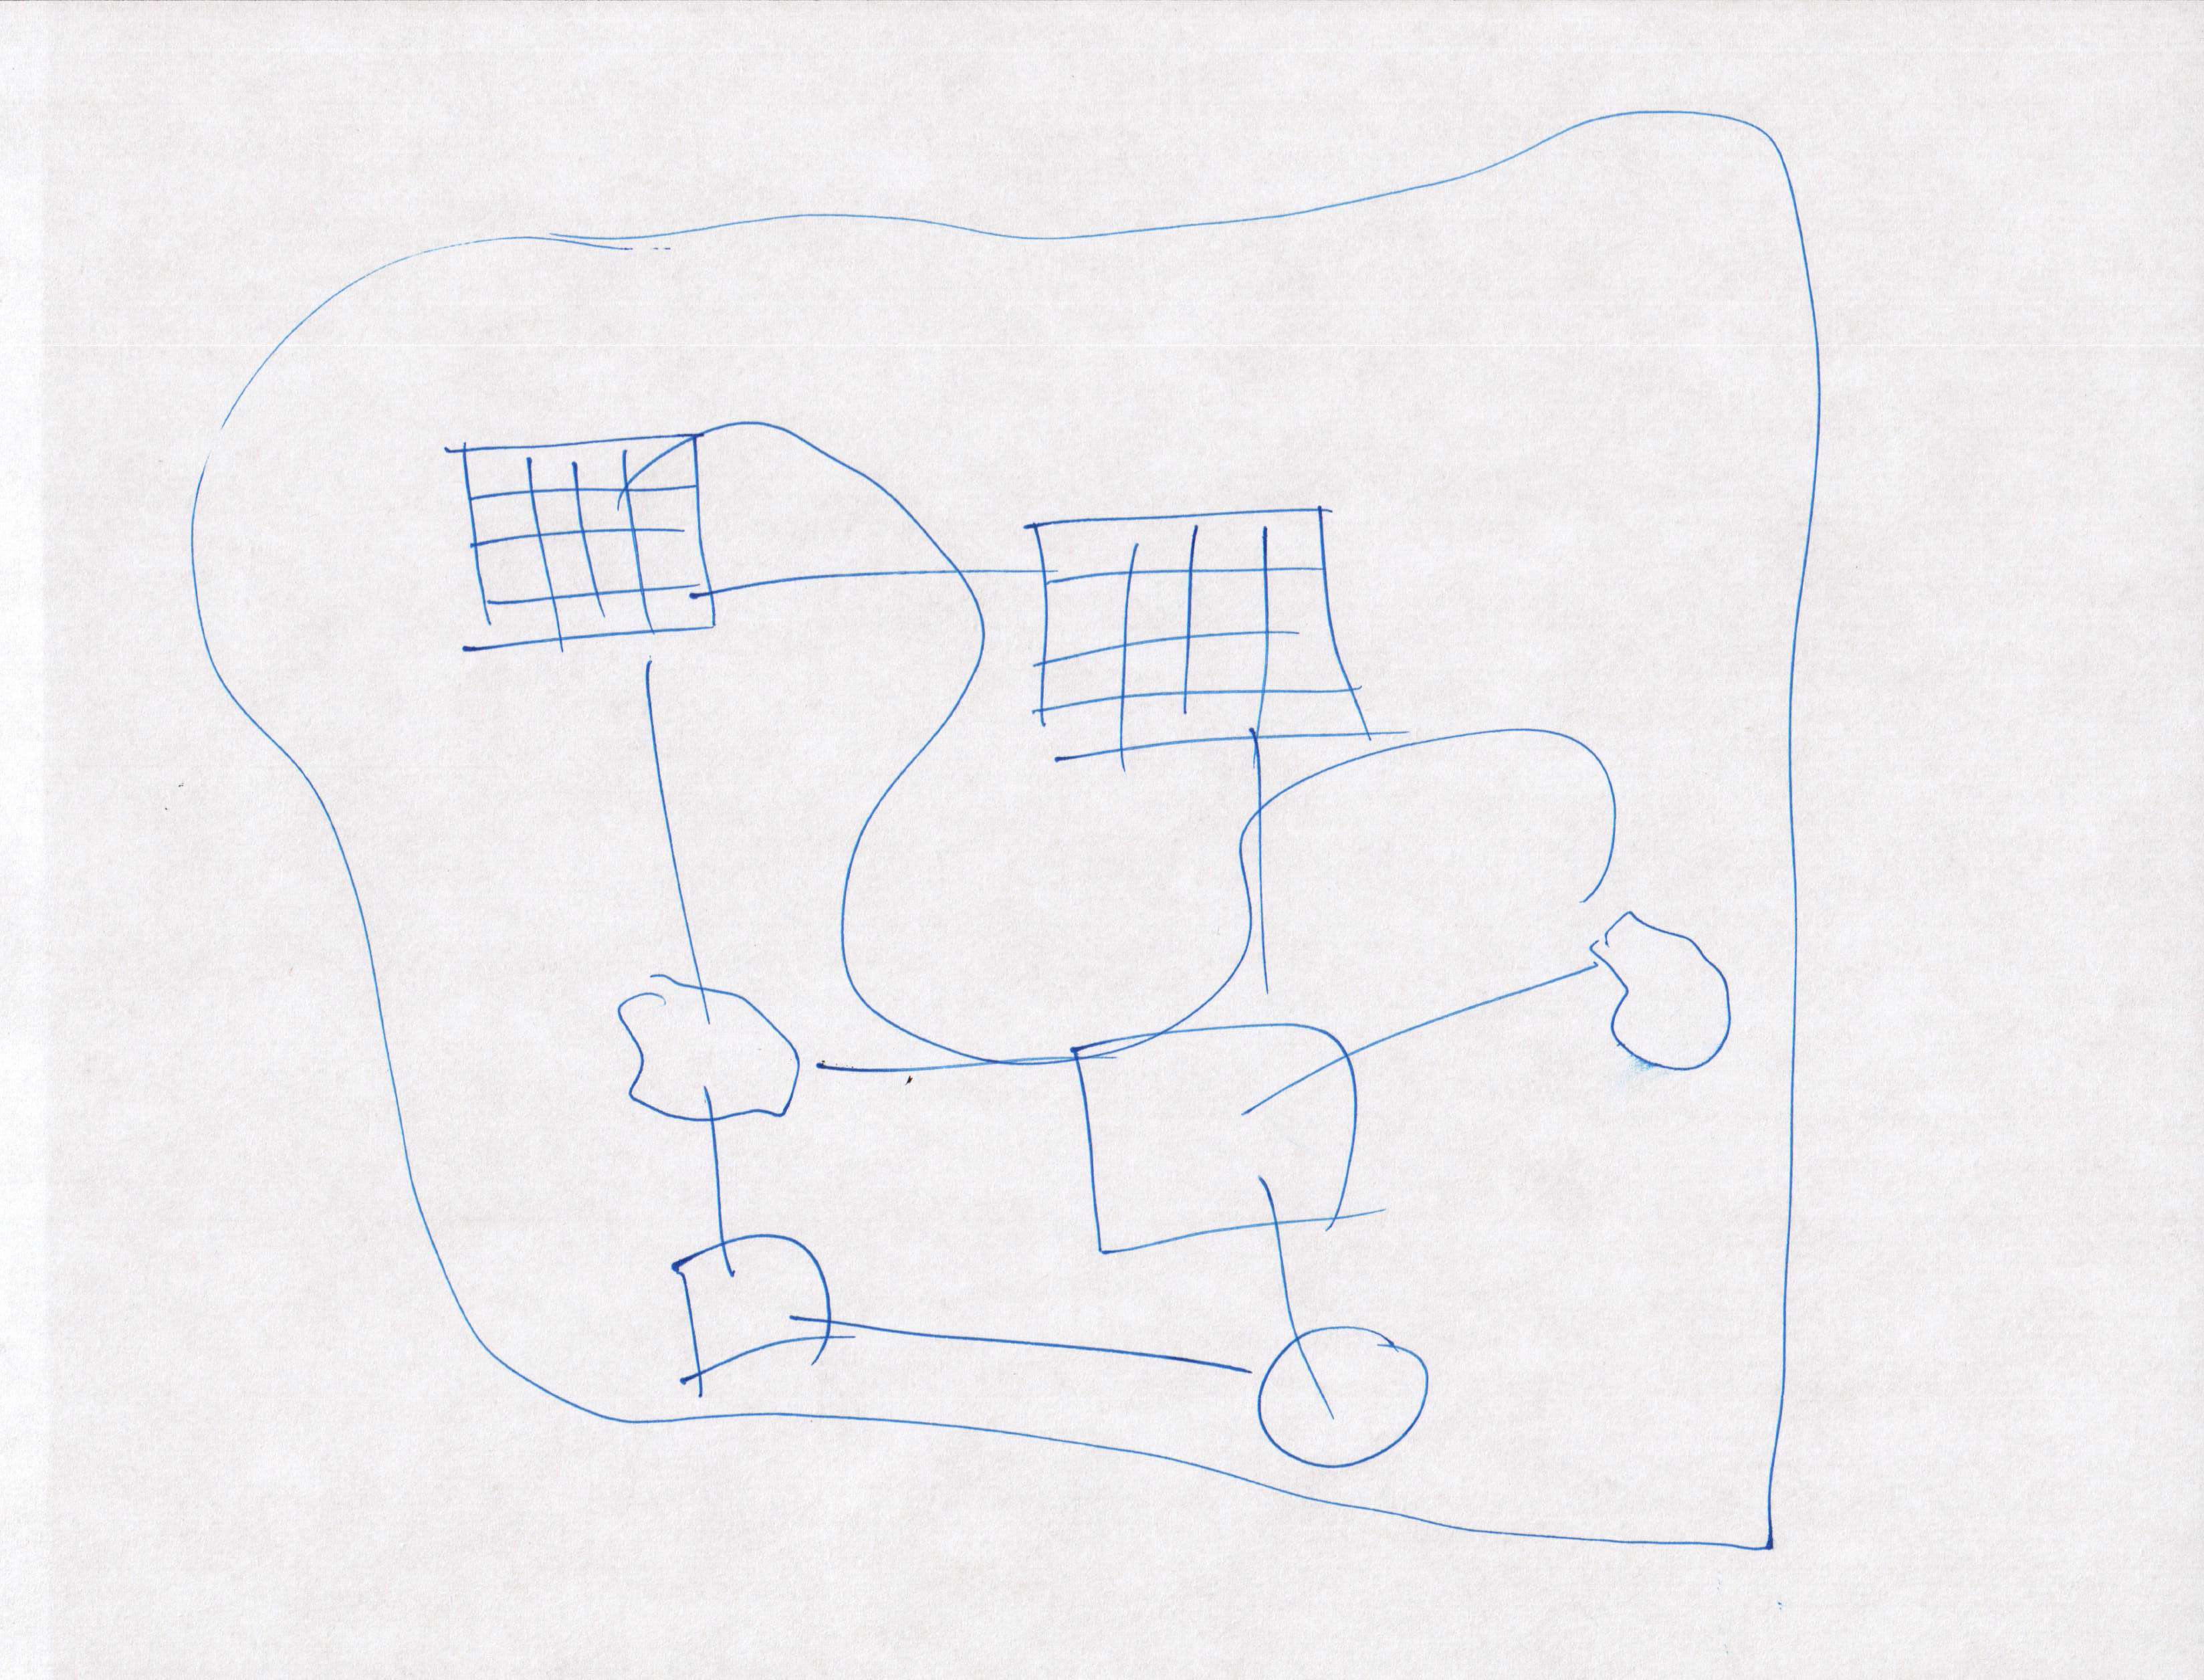
\includegraphics[width=3.45in]{team_code_ownership_images/CodeOwnership.jpg}
\caption{\quotes{Draw how you feel about the code}}
\label{Programmer1}
\end{figure}

The team wants to feel pride in improving code quality.  It feels good to be improving the code design and readability. If the team starts neglecting these concerns, it can engender a sense of disgust and apathy for the code can spread throughout the team.

\subsection{Product Fit}
\textbf{Definition:} Product fit is developers believing that features of the product will satisfy the user's needs.

\textbf{Purpose:} Engineers want to create products that matter to the users. Delivering a product that matters to someone satisfies the self-identity motivation of psychological ownership.

\textbf{Threat: Ignoring user feedback.} When the product manager ignores feedback from user research and usability testing, developers may lose faith in the product's ability to achieve its goals. Developer motivation and engagement can decrease when developers perceive they are building a feature that users have explicitly said they do not want yet is built to solve a business goal. 

\textbf{Threat: Ignoring developers feedback about the product.} Pivotal's balanced team approach is founded on collaboration between product managers, interaction designers, and developers. When product managers or other stakeholders ignore feedback from developers, developers can begin to feel less ownership in the product, and in turn, be less motivated to work on the project. 

%When picking up a story, a developer verifies that the story contains clear acceptance criteria. In the absence of acceptance criteria, the developer typically clarifies what needs to be done with the product manager. On one project during which the stakeholders ignored feedback from the developers, one developer recalled, \participantQuote{In this case, I don't feel like spending the extra energy to go and say, `Hey, are you sure? Is this what you want?'} 

Feature apathy or product apathy can result in a poorly crafted product that does not meet the customer's needs.

\subsection{Team Cohesion}
\textbf{Definition:} Team cohesion is the degree to which team members identify as part of the team, stick together through adversity and take pride in the team's accomplishments \cite{Bollen1990Perceived, Beal2003Cohesion, Whitworth2007Motivation}.

\textbf{Purpose:} Team cohesion satisfies the \quotes{having a place} motivation of psychological ownership.

\textbf{Threat: Distancing a developer from the team.} Team apathy manifests when developers do not feel that they are a part of the team. Developers feel less ownership of the code base when they feel excluded from the team.

Several behaviors were observed that can distance a developer from the team: interrupting the developer during discussions, using poor listening skills so that the developer feels unheard, or talking beyond the developer's level of technical expertise. 

On one team, during discussions, the team talked about code but never looked at the source code. One developer found these abstract discussions difficult to follow. Sometimes the team discussed parts of the code that the individual had not seen recently. When the team discussed two variants of coding practices without showing concrete examples, the programmer could not contribute. When the developer raised this issue to the team and the team continued with the status quo, the programmer felt marginalized by the team.

Poor onboarding of developers can contribute to feelings of isolation. On one project, there was a time crunch and the team was feeling the pressure to deliver stories. When the team added developers, the team had a \quotes{sink or swim} attitude, letting new team members figure things out on their own, hence making them feel unwelcome.

When developers feel that the team does not care about them, their sense of ownership can decrease.

\section{Discussion}
\label{Discussion}
\subsection{Transitioning to team code ownership}
\label{Transitioning}

The above results have numerous implications for teams attempting to transition to team code ownership. 

Some developers effortlessly make the transition to team code ownership. They immediately see the benefits of being able to modify any part of the code base and quickly shift from \quotes{I made this} (personal ownership) to \quotes{we made this} (collective ownership.)

Others may struggle with team code ownership for several reasons:

\begin{itemize}  

\item Developers may struggle to transition to a caretaker mindset.  In one interview, a software engineer struggled to describe the developer's relationship with the code on a very challenging project and settled in on the caretaker metaphor: \participantQuote{Sometimes I kind of feel like a janitor to [the code base].  Maybe caretaker would be better. Yeah, probably caretaker. I feel like a janitor just cleans up messes, but a caretaker makes things better.} 

\item A developer may be distraught at \participantQuote{seeing my work slowly removed from the app.} 

\item Developers can no longer take pride in functionality that they exclusively develop.

\item Existing knowledge silos, which hinder team code ownership, may be slow to break down.
 
\end{itemize}

New hires struggling with the transition slowly realize that \participantQuote{someone else is going to take over and they're going to do fine. I can move onto something else and that's okay.} They recognize the lack of long-term individual authorship, learn to expect their code to be transitory, develop trust in their teammates and thus loosely hold personal contributions. \participantQuote{The code that I write today may be in the code base for a little while, and it will evolve into something better.} Eventually,  they experience the benefits of a collaborative environment: \participantQuote{People are a lot more flexible all across the board, with changing things or accepting feedback or collaborating,} and the team can say \quotes{Hey, this is our code!}

Shifting from individual to team code ownership may requires multiple and complementary practices to actively remove knowledge silos. In this case, daily pair rotation helped combat knowledge silos. Moreover, for developers with strong individual ownership tendencies, sharing ownership first with a small group (where trust and communication come easier) may help. One Pivotal engineer uses improvisation and collaboration games to help teams practice letting go of control, trusting the team, and learning to be pleasantly surprised by what emerges. 

\subsection{Results Evaluation}

The factors influencing team code ownership presented in Section \ref{TeamCodeOwnership}, have emerged from the Grounded Theory research study introduced in Section \ref{SustainableSoftwareDevelopmentTheory}. While other factors may influence team code ownership, this discussion focuses only on those that were observed during the study. Grounded Theory studies can be evaluated using the following criteria \cite{Charmaz}: 

\textbf{Credibility:}  The \numberOfInterviews{} intensive open-ended interviews and numerous field notes from participant-observation serve as a rich and credible data set for the analysis. 

\textbf{Originality:} The research broadens the idea of team code ownership by acknowledging that collective code ownership is more than a policy statement, and by uniquely identifying factors that affect the team's sense of code ownership.

\textbf{Resonance:} Several participants reviewed the findings and indicated that both the factors and threats resonate with their experience.

\textbf{Usefulness:} The study identifies factors associated with ownership and suggests several ways of engendering team code ownership.

This work analyzed software projects at the Silicon Valley office of Pivotal following Extreme Programming. From an \textbf{external validity} perspective, grounded theory is non-statistical, non-sampling research. The results therefore cannot be statistically generalized to a population. Rather, researchers and professionals can adapt the concepts and ideas to other contexts case-by-case. 

Finally, the results might be influenced by \textbf{researcher bias} or \textbf{prior knowledge bias}. A risk of the participant-observer technique is that the researcher may lose perspective and become biased by being a member of the team. While a participant-observer gains perspective an outsider cannot, an outside observer might see something a participant observer will miss. Similarly, while prior knowledge helps the researcher interpret events and select lines of inquiry, prior knowledge may also blind the researcher to alternative explanations \cite{GlaserIssues}. These risks were mitigated by recording interviews and having the researchers review the coding process. 

\section{Conclusion}
\label{TeamCodeOwnershipConclusion}
This chapter reports results from a participant-observation, constructivist grounded theory study at Pivotal, a large American software company employing Extreme Programming practices. It provides three main contributions.

1) The observations clearly indicate that \textbf{team code ownership is a feeling to be engendered not a policy to be decreed}.

2) Meanwhile, both discussions with and observations of participants suggest five factors associated with strong feelings team code ownership. Pivotal developers more acutely feel team code ownership when i) they understand the system context; ii) they have contributed to the code in question; iii) they perceive code quality as high; iv) they believe the product will satisfy user needs; and v) they perceive team cohesion as high.   

3) Moreover, diverse events and trends can undermine sense of ownership, including:  increasing knowledge silos, increasing code base size, increasing team size, inability to contribute, pressure to deliver and deprioritizing continuous refactoring, ignoring user feedback, ignoring developer feedback, and distancing a developer from the team. 

In conclusion, Pivotal's developers find team code ownership highly advantageous; however, transitioning to a team code ownership model is easier for some than others. Some agile practices including continuous pair programming, overlapping pair rotation, continuous refactoring, and test driven development appear to help. Promising angles for future research include more nuanced explorations of the code ownership spectrum, further exploration of the roles of emotion and identity, as well as developing specific practices for facilitating ownership transitions. 



\chapter{Removing Waste}
\label{SoftwareEngineeringWasteChapter}
\section{Summary}

\textit{Context:} Software development is a complex socio-technical activity that involves coordinating different disciplines and skill sets and thus provides ample opportunity for waste to emerge. Waste is any activity that produces no value for the user.
\textit{Objective:} The purpose is to understand observed wastes in software development.
\textit{Method:} Following Constructivist Grounded Theory, we conducted a two-year participant-observation of several software development projects at Pivotal, interviewed \numberOfInterviews{} software engineers, interaction designers, and product managers, and analyzed one year of retrospection topics. We iterated between analysis and theoretical sampling until achieving theoretical saturation.
\textit{Results:}  This chapter introduces the first evidence-based waste taxonomy, identifying eight wastes along with causes and tensions within wastes. It also compares this study's taxonomy with the waste taxonomy found in Lean Software Development.
\textit{Limitations:} While the results are highly relevant to Pivotal, the outcomes might not apply to organizations with different software development cultures.
\textit{Conclusion:} The waste taxonomy serves as a starting point for waste identification and elimination. Comparing this taxonomy to Lean Software Development's list of wastes revealed our taxonomy's parsimony and expressiveness while illustrating wastes not covered by previous work. 

\section{Introduction}
\participantQuote{The engineers are depressed. The project grinds them down\ldots It is hard to know which problem to tackle first. There is coupling everywhere\ldots Each layer of the system has unnecessary complexity\ldots The depth of knowledge about the system is super thin\ldots There is a lot of waiting\ldots Building the java code takes ten minutes. Starting the server takes seven minutes. Running the javascript tests take two minutes. Running the integration tests take 47 minutes. Continuous integration takes \textit{forever} to run all the tests and get the code onto the acceptance environment. \newline \indent There is waste everywhere. \textemdash Software Engineer on Project Septem}

Software development is a complex socio-technical activity that involves coordinating different disciplines and skill sets. Identifying user needs, crafting features for those needs, identifying and prioritizing value, implementing features, releasing and supporting products provide ample opportunity for waste to creep in. 

Here, \quotes{waste} refers to \quotes{any activity that consumes resources but creates no value} for customers \cite{WomackLeanThinking}. Eliminating waste, by definition, improves efficiency and productivity. 

However, eliminating waste can be difficult not least because \textit{identifying} waste can be difficult.  Numerous cognitive phenomena including status quo bias \cite{JostDecadeOfSystemJustification} hinder practitioners' propensity and ability to notice waste in existing practices. Identifying the types of waste that often occur in software projects  may, therefore, facilitate our ability to identify and eliminate waste. Identifying and eliminating waste is a key principle of lean manufacturing. 

The Toyota Production System \cite{OhnoToyotaProductionSystem, ShingoToyotaProductionSystem} transformed manufacturing from batch-and-queue to just-in-time. The similarities between batch-and-queue and waterfall, as well as just-in-time and iterative software development, inspired several software development methods \cite{PoppendieckLeanSoftwareDevelopment, AndersonKanban}. These methods adapt, in a top-down fashion, lean principles for software environments. 

However, manufacturing differs from software development in significant ways. Software is intangible and practically free to duplicate. Two customers can buy the same software in a way they cannot buy the same car. A software developer can produce a wider variety of products than an assembly line. While most factories build batches of near-identical goods, much software remains unique. The cost structure is fundamentally different since the variable costs of software are near zero, while cars have high variable cost and higher fixed costs for factories. 

Given the obvious differences between developing software and manufacturing physical products, software development may entail waste types never envisioned by the literature on lean manufacturing. Even the most careful adaptation of lean principles for software may not have identified such waste types. Therefore, we report an in-depth, longitudinal investigations of a successful software company to address the following research question: 

\textbf{Research Question: \quotes{What are observed wastes in software development?}}

Any software development process does instill repeated activities such as taking a story off a backlog or writing test cases which can be optimized. One goal would be to make these processes efficient and repeatable in a similar context. 

Section \ref{HistoryOfLean} briefly reviews the history of lean in and Section \ref{RelatedWork} reviews related work. Section \ref{ResearchMethod} describes the research method. Section \ref{SEWaste} presents the emergent waste taxonomy. Section \ref{LeanSoftwareDevelopmentComarison} compares this model with the waste list from Lean Software Development. Sections \ref{ResultsEvaluation} and \ref{Conclusion} evaluates the results, presents limitations, and concludes the paper.

\section{A Brief History of Lean}
\label{HistoryOfLean}

The Toyota Production System prioritizes waste removal by creating a culture that pursues waste identification and elimination in the entire production of a vehicle \cite{OhnoToyotaProductionSystem, ShingoToyotaProductionSystem}. In 1945, Toyota optimized for the production rate of each system, keeping like machines near each other. Ohno rearranged equipment so that the output of one machine fed into the next machine, slowed machines down to have the same cadence, and only produced material when it was needed. After optimizing Toyota's factories, Toyota then trained their suppliers so that the entire production of a vehicle was just-in-time, transforming from mass production to lean production. The resulting \quotes{pull} system was easy to reconfigure, minimized inventory, and supported short production runs.  

Based on analysis of the Toyota Production System, Lean Thinking \cite{WomackLeanThinking} describes a process of identifying and removing waste using five principles:
\begin{enumerate}
\item Specify value: define value from the customer's perspective
\item Identify the value stream: examine all actions required to bring raw materials to final product for the customer and eliminate any obvious unnecessary steps
\item Flow: re-engineer from batch-and-queue to just-in-time or continuous flow 
\item Pull: create products only in response to a customer order
\item Perfection: continue with a continuous process of waste identification and elimination
\end{enumerate}

Analyzing the value stream involves identifying three types of activities: activities that clearly create value; activities that create no value for the customer but currently necessary to manufacture the product; and activities that create no value for the customer, are unnecessary and therefore should be removed immediately, i.e., waste.

The Toyota Production System characterized seven types of manufacturing waste \cite{ShingoToyotaProductionSystem} shown in Table \ref{ManufacturingWaste}. Later, Womack and Liker each added a waste type \cite{WomackLeanThinking, LikerToyotaWay}.

\begin{table}[t]
\renewcommand{\arraystretch}{1.5}
\centering
\caption{Toyota Production System Definition of Manufacturing Waste}
\label{ManufacturingWaste}
\begin{tabular}{|p{2in}|p{4in}|}
% \begin{tabular}{|p{0.85in}|p{2.3in}|}
\hline

Waste Type                & Description                                                                                                                                                  \\ \hline
Inventory                 & The cost of storing materials until they are needed. Sometimes the material is never used.                                                                   \\ \hline
Extra Processing          & The cost of processing that is not needed by a downstream step in the manufacturing process. (Sometimes an inefficiency from not seeing the entire process.) \\ \hline
Overproduction            & The cost of producing more quantity of components than necessary for the present.                                                                            \\ \hline
Transportation (of goods) & The cost of unnecessarily moving materials from one place to another place.                                                                                  \\ \hline
Waiting                   & The cost of waiting for a previous upstream step to finish.                                                                                                       \\ \hline
Motion (of people)        & The cost of unnecessary picking up and putting things down.                                                                                                  \\ \hline
Defects                   & The cost of rework from quality defects.                                                                                                                     \\ \hline
Value                     & The cost of producing goods and services that do not meet the needs of the customer.                                                                         \\ \hline
Non-utilized Talent       & The cost of unused employee creativity and talent.                                                                                                           \\ \hline
\end{tabular}
\end{table}

\section{Related Work}
\label{RelatedWork}
We could not find any evidence-based publications on software engineering waste. This section provides one non-empirical waste taxonomy followed by several observational studies that applied Value Stream Mapping to software development.

Mary and Tom Poppendieck contributed the most influential body of work in the area of software waste. In creating Lean Software Development \cite{PoppendieckLeanSoftwareDevelopment}, the Poppendiecks adapted Lean Thinking and the Toyota Production System from manufacturing to software development. Their comparison of manufacturing waste with software waste is presented in Table \ref{ManufacturingVersusLeanSoftwareWaste}.
 
\begin{table}[t]
\renewcommand{\arraystretch}{1.5}
\centering
\caption{Comparison of Manufacturing Waste with Lean Software Development Waste}
\label{ManufacturingVersusLeanSoftwareWaste}
\begin{tabular}{|l|l|}
\hline
Toyota Production System's Manufacturing Wastes & Poppendieck's Software Development Wastes \\ \hline
Inventory                                       & Partially Done Work                       \\ \hline
Extra Processing                                & Relearning                                \\ \hline
Overproduction                                  & Extra Features                            \\ \hline
Transportation (of goods)                       & Handoffs                                  \\ \hline
Waiting                                         & Delays                                    \\ \hline
Motion (of people)                              & Task Switching                            \\ \hline
Defects                                         & Defects                                   \\ \hline
Value (added by Womack in 1996)                 & N/A                                       \\ \hline
Non-utilized Talent (added by Liker in 2004)     & N/A                                       \\ \hline
\end{tabular}
\end{table}

The Poppendieck's mapping is top-down in the sense that they ask, what is the equivalent of each type of manufacturing waste in a software context. However, some types of manufacturing waste (e.g., transportation and motion) which rely on physical attributes may not map well to software development which is intangible while software development may exhibit new types of waste not present in manufacturing. This motivates a complementary bottom-up empirical research in software development contexts to identify and characterize different types of waste. 

The Poppendiecks suggest \quotes{the five biggest causes of policy-driven waste:} complexity, economy of scale, separating decision making from work, wishful thinking, and technical debt \cite{PoppendieckResultsNotPoint}.

Power and Conboy leverage the Poppendieck's model by combining it with literature in manufacturing, lean production, product development, construction, and healthcare. They shift from using wastes of inefficiencies to impediments to flow. \cite{PowerImpediments}

Petersen and Wohlin examined the flow of features by creating cumulative flow diagrams through the different development phases at Ericsson AB in Sweden and India. (The phases are detailing features, implementing and unit testing features, isolation testing, system testing, and ready for release.) They defined several metrics to identify bottlenecks, variance in hand-overs, and cost types. For cost savings analysis, they define waste as any feature that has work done on it (e.g. \quotes{describing the feature}) but is never released to a customer \cite{Petersen2011}.

Several studies applied Value Stream Mapping to software development. Value Stream Mapping popularized by Womack systematically examines each stage for waste. Interestingly, these studies only found the waste of waiting rising from a batch-and-queue system \cite{Ali2016, Khurum2014, Mujtaba2010}. One study identified the wastes of motion and extra processing from interviews, not the current state map \cite{Mujtaba2010}.

Khurum said, \quotes{the researchers found it is more suitable to start focusing on improvement potential based on long waiting or lead time.} During the waste identification step of the workshop with their research participants, they ask attendees \quotes{in which phase do we see the majority of waiting?} \cite{Khurum2014} The Pygmalion effect (self-fulfilling prophecy) may explain why the researchers only found \textit{waiting} waste in Value Stream Mapping analysis.

Ali et al applied information flow modeling to Value Stream Mapping which revealed \textit{waiting} waste from the passing of big batches from group to group and missing prioritization \cite{Ali2016}.

These studies typically reduced waste by switching the organization from waterfall to iterative software development or reducing the batch size in iterative software development \cite{Ali2016, Khurum2014, Mujtaba2010}.

% \section{Research Method}
% \label{ResearchMethod}
% \subsection{Constructivist Grounded Theory}
% We used Constructivist Grounded Theory \cite{Charmaz}, which involves iteratively collecting and analyzing data to generate and refine an emergent theory. Grounded Theory research begins by asking, \quotes{What is happening here?} \cite{GlaserTheoreticalSensitivity}; or in this case, \quotes{What is happening at Pivotal when it comes to software development?} \textit{Removing Waste}  later emerged as a core category.
% \subsection{Research Context: Pivotal Labs}
% Pivotal Labs is a division of Pivotal\textemdash a large American software company (with 17 offices around the world). Pivotal Labs provides teams of agile developers, product managers, and interaction designers to other firms. Its mission is not only to deliver highly-crafted software products but also to help transform clients' engineering cultures. To change the client's development process, Pivotal combines the client's software engineers with Pivotal's engineers at a Pivotal office where they can experience Extreme Programming \cite{BeckExtremeProgramming2004} in an environment conducive to agile development. 

% Typical teams include six developers, one interaction designer, and a product manager. The largest project in the history of the Palo Alto office had 28 developers while the smallest had two. Larger projects are organized into smaller coordinating teams with one product manager per team and one or two interaction designers per team.

% Interaction designers identify user needs predominately through user interviews; create and validate user experience with mockups; determine the visual design of a product; and support engineering during implementation. Product managers are responsible for identifying and prioritizing features, converting features into stories, prioritizing stories in a backlog, and communicating the stories to the engineers. Software engineers implement the solution. 

% Pivotal Labs has followed Extreme Programming \cite{BeckExtremeProgramming2004} since the late 1990's. While each team autonomously decides what is best for each project, the company culture strongly suggests following all of the core practices of Extreme Programming, including pair programming, test-driven development, weekly retrospectives, daily stand-ups, a prioritized backlog, and team code ownership. We only observed teams at Pivotal Labs. Other teams, especially teams in other divisions, might have a different culture and follow different software practices.
% \subsection{Data Collection}
% This discussion analyses data from three sources: 1) interviews with Pivotal employees, 2) topics discussed in 91 retrospection meetings, and 3) participant observation of \numberOfObservedProjects{} projects over two years. To preserve client confidentiality, we can only reveal limited information about each project:

% \begin{itemize}
% \item Project Unum (two product managers, four developers) was a greenfield project providing a web front end for installation, configuring, and using a multi-node cluster with big data tools. 
% \item Project Duo (two interaction designers, two product managers, six developers) added features to a print-on-demand e-commerce platform. 
% \item Project Tes (one interaction designer, one product manager, six developers) added features to management software for internet service providers.
% \item Project Quattuor (two interaction designers, three product managers, 28 developers) developed two mobile applications and a backend system for controlling expensive equipment.
% \item Project Kvin (one interaction designer, one product manager, six developers) was a greenfield project for a healthcare startup. 
% \item Project Ses (two interaction designers, one product manager, ten developers) was adding features and removing technical debt to an existing internet e-commerce website.
% \item Project Septem (two interaction designers, three product managers, twelve developers) was adding features and removing technical debt to an existing virtual machine management software.
% \end{itemize}
% \subsubsection{Participant Observation}
% The first author collected field notes while working as an engineer on all \numberOfObservedProjects{} projects. These notes describe individual and collective actions, capture what participants found interesting or problematic, and include anecdotes and observations.
% \subsubsection{Interviews}
% The first author interviewed \numberOfInterviews{} interaction designers, product managers, and software engineers who had experience with Pivotal's software development process from five different Pivotal offices. Participants were not paid for their time.

% We relied on \quotes{intensive interviews,} which are \quotes{open-ended yet directed, shaped yet emergent, and paced yet unrestricted} \cite{Charmaz}. Open-ended questions were used to enter into the participant's personal perspective within the context of the research question. The interviewer attempts to abandon assumptions to better understand and explore the interviewee's perspective. Charmaz \cite{Charmaz} contrasts intensive interviews with informational interviews (collecting facts), and investigative interviews (exposing hidden intentions, practices or policies).

% The initial interviews were open-ended explorations starting with the question, \quotes{Please draw on this sheet of paper your view of Pivotal's software development process.} The interviewer specifically did not force initial topics and merely followed the path of the interviewee. While exploring new emergent core categories, whenever possible, we initiated subsequent interviews with open-ended questions. The first author transcribed each interview with timecode stamps for each segment. These interviews were spread across the duration of the research study. 
% \subsubsection{Retrospection Topics}
% When \textit{removing waste} emerged as a core category from interviews and participant observation, we began collecting data from retrospection meetings. A retrospection meeting (or retro) is a meeting to pause, reflect, and discuss the work done during the week, i.e., a safe place where any team member can discuss any issue \cite{DerbyAgileRetrospectives}. Retros are typically scheduled every Friday afternoon. The entire team and important stakeholders attend these meetings. 

% The observed Pivotal teams mostly use an emotion-based retro format where \quotes{happy,} \quotes{meh,} and \quotes{sad} faces are written on the top of a whiteboard. The happy-face column represents items that are working well, of which the team wants to do more. The meh-face column represents  items that the team needs to \quotes{keep an eye on.} The sad-face column represents items that are not working well, which the team should try to fix. Any team member can add any topic to any column. After a few minutes, the team dot-votes on the topics to discuss \cite{DerbyAgileRetrospectives}. The team uses the remainder of the sixty-minute meeting to discuss topics. Sometimes discussing a topic is sufficient to affect change, other times the team creates action items. 

% We collected data from 91 retrospection meetings over 59 weeks from Projects Quattuor, Kvin, and Ses. (There are more meeting than weeks since each of Project Quattuor's three teams held its own retro each week.)

% For co-located teams, the first author took a picture of the whiteboard at the end of the retro and later transcribed the topics into a master spreadsheet. For distributed teams, we copied data from the on-line spreadsheets the team used in place of a whiteboard. Attendees often wrote a short phrase as a proxy for a larger idea. For example, \quotes{Scope} represents \quotes{Too much scope is causing the team stress} or \quotes{Legal} represents \quotes{Waiting on Legal to approve the legal process.} When the provided topic was too vague, we solicited a more detailed description from an engineer present in the meeting. This produced 663 total items for analysis. 
% \subsection{Data Analysis}
% We began by iteratively collecting and analyzing interview transcripts and participant observations. We used line-by-line coding \cite{Charmaz} to identify nuanced interactions in the data and avoid jumping to conclusions. We reviewed the initial codes while reading the transcripts and listening to the audio recordings. We discussed the coding during weekly research collaboration meetings. To avoid missing insights from these discussions \cite{GlaserTheoreticalSensitivity}, we recorded and transcribed them into grounded theory memos. As data was collected and coded, we stored initial codes in a spreadsheet and we used constant comparison to generate focused codes.

% We routinely compared new codes to existing codes to refine codes and eventually generate categories. We periodically audited each category for cohesion by comparing its codes. When this became complex, we printed codes on index cards, and then arranged and re-arranged until cohesive categories emerged. We wrote memos to capture the analysis of codes, examinations of theoretical plausibility, and insights.

% When \textit{removing waste} appeared as a core category, we began collecting and analyzing data from retrospectives to investigate (theoretical sampling). After removing irrelevant topics (e.g. complaints about the weather), we printed each retro item onto an index card with its original retro topic, enhanced description, id, and team name (see Figure \ref{exampleRetroTopicl}).

% Over the course of two days, two researchers with first-hand experience of the projects did initial coding of the retro topics and merged duplicate topics. We rearranged initial coding categories to be near similarly themed categories and iteratively combined and reorganized categories (see Table \ref{ChainOfEvidence} for example classification). We often stopped to record new insights. When the categories began to stabilize, we compared each category against the other categories looking for relationships. Once we felt that the categories were stable, we performed a final review of each category to verify that the cards belonged to it. 

% We continued theoretical sampling for removing waste in additional interviews and participant observations until no further waste-related categories were evident, i.e. theoretical saturation. 


% \begin{table}[t]
% \renewcommand{\arraystretch}{1.5}
% \centering
% \captionof{figure}{Example Retro Topic Index Card }
% \label{exampleRetroTopicl}
% \begin{tabular}{|l|}
% \hline
% Topic: Legal \\ \\ Description: Waiting on Legal to approve legal pages \\ \\ Id: 182 Project: Quattour\\ \hline
% \end{tabular}
% \end{table}








\begin{table}[ht]
\centering
\captionof{figure}{Examples for Cognitive Hindrance Waste}
\label{ChainOfEvidence}
\begin{tabular}{|llll|}
\hline
\multicolumn{4}{|l|}{}  \\
\multicolumn{4}{|l|}{\underline{Waste Category}: Cognitive hindrance}  \\
    & \multicolumn{3}{l|}{\textbf{Cause Category}: Emotional stress}          \\
    &     & \multicolumn{2}{l|}{\textit{Cause Property}: Low team morale} \\
    &     &      & Retro Topic: Frustrated clients / Pivotal developers       \\
    &     &      & Retro Topic: Negative attitudes                \\
    &     &      & Retro Topic: Apathy                            \\
    &     &      & Retro Topic: Unacknowledged by management      \\
    &     &      & Retro Topic: Messy code                        \\
    &     &      & Retro Topic: Pairing fatigue                   \\
    &     &      & Retro Topic: Poor lighting, lack of windows    \\
    &     & \multicolumn{2}{l|}{\textit{Cause Property}: Rush mode} \\
    &     &      & Retro Topic: Fixed features with a fixed timeline \\
    &     &      & Retro Topic: Aggressive timelines \\
    &     &      & Retro Topic: Scope creep \\
    &     &      & Retro Topic: Repeatedly saying \quotes{This has to be done today} \\
    &     &      & Retro Topic: Long days \\
    &     &      & Retro Topic: Overtime \\
    &     & \multicolumn{2}{l|}{\textit{Cause Property}: Lack of empathy} \\
    &     &      & Retro Topic: Not listening \\
    &     &      & Retro Topic: Criticizing in public \\
    &     &      & Retro Topic: Difficult pairings \\
    &     &      & Retro Topic: Interpersonal conflict \\
    &     &      & Retro Topic: Kicking product out of the team space \\
    & \multicolumn{3}{l|}{\textbf{Cause Category}: Cognitive load}          \\
    &     & \multicolumn{2}{l|}{\dots} \\
    & \multicolumn{3}{l|}{\textbf{Cause Category}: Context Switching}          \\
    &     & \multicolumn{2}{l|}{\dots} \\
\hline
\end{tabular}
\end{table}

\section{Results: Types of Waste in Software Engineering}
\label{SEWaste}

% \begin{figure}[t]
% \centering
% \captionof{table}{Types of Software Development Waste}
% \label{Waste}
% 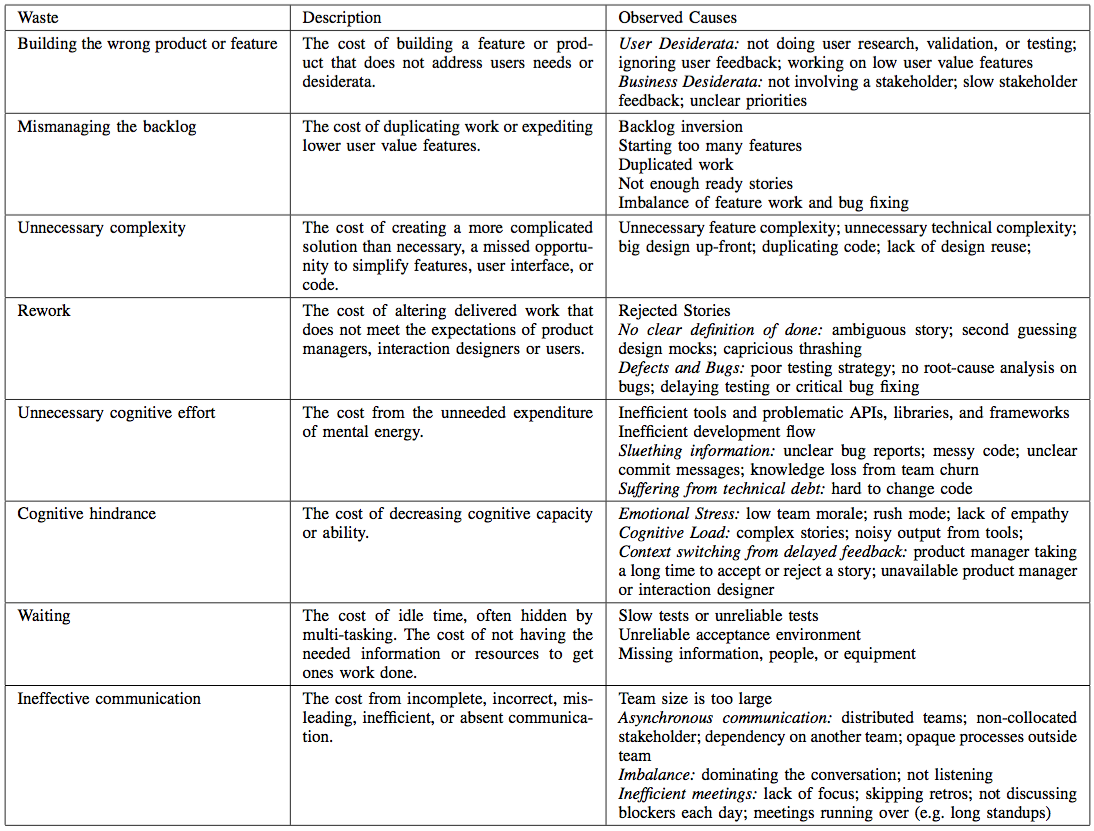
\includegraphics[width=6.4in]{software_engineering_waste/waste.png}
% \end{figure}

\begin{table*}[htbp]
\renewcommand{\arraystretch}{1.3}
\centering
\caption{Types of Software Development Waste}
\label{Waste}
\begin{tabular}{|p{2.5in}|p{3.6in}|} %dissertation size
\hline
\textbf{Waste} \newline Description                                                                                                         & Observed Causes                                                                                                                                                                                                                                                                                                                                                                                                                     \\ \hline
\textbf{Building the wrong feature or product} \newline
The cost of building a feature or product that does not address user's needs or desiderata.                                  & \textit{User Desiderata:} not doing user research, validation, or testing; ignoring user feedback; working on low user value features \newline \textit{Business Desiderata:} not involving a stakeholder; slow stakeholder feedback; unclear priorities                                                                                                                                                                                  \\ \hline
\textbf{Mismanaging the backlog  } \newline The cost of duplicating work or expediting lower user value features.                                                       & Backlog inversion \newline Starting too many features \newline Duplicated work \newline Not enough ready stories  \newline Imbalance of feature work and bug fixing                                                                                                                                                                                                                                                                                                                                      \\ \hline
\textbf{Unnecessary complexity} \newline The cost of creating a more complicated solution than necessary,  a missed opportunity to simplify features, user interface, or code.      & Unnecessary feature complexity; unnecessary technical complexity; big design up-front; duplicating code; lack of design reuse;                                                                                                                                                                                                                                                                                                                 \\ \hline
\textbf{Rework } \newline The cost of altering delivered work that does not meet the expectations of product managers, interaction designers or users.    & Rejected Stories \newline \textit{No clear definition of done:} ambiguous story; second guessing design mocks; capricious thrashing \newline \textit{Defects and Bugs:} poor testing strategy; no root-cause analysis on bugs; delaying testing or critical bug fixing                                                                                                                                                                    \\ \hline
\textbf{Unnecessary cognitive effort} \newline   The cost from the unneeded expenditure of mental energy.                                                                                                                 & Inefficient tools and problematic APIs, libraries, and frameworks  \newline Inefficient development flow \newline \textit{Sluething information:} unclear bug reports; messy code; unclear commit messages; knowledge loss from team churn \newline\textit{Suffering from technical debt:} hard to change code
                                                                     \\ \hline
\textbf{Cognitive hindrance} \newline The cost of decreasing cognitive capacity or ability.                        & \textit{Emotional Stress:} low team morale; rush mode; lack of empathy \newline \textit{Cognitive Load:} complex stories; noisy output from tools; \newline \textit{Context switching from delayed feedback:} product manager taking a long time to accept or reject a story; unavailable product manager or interaction designer                                                                                                                                                        \\ \hline
\textbf{Waiting} \newline The cost of idle time, often hidden by multi-tasking. The cost of not having the needed information or resources to get one's work done. & Slow tests or unreliable tests \newline Unreliable acceptance environment \newline Missing information, people, or equipment                                                                                                                                                                                                                                                                            \\ \hline
\textbf{Ineffective communication} \newline The cost from incomplete, incorrect, misleading, inefficient, or absent communication.                         & Team size is too large \newline \textit{Asynchronous communication:} distributed teams; non-collocated stakeholder; dependency on another team; opaque processes outside team \newline \textit{Imbalance:} dominating the conversation; not listening \newline \textit{Inefficient meetings:} lack of focus; skipping retros; not discussing blockers each day; meetings running over (e.g. long standups) \\ \hline                  
\end{tabular} 
\end{table*}

We identified eight types of waste listed in Table \ref{Waste}. The table lists the waste type, a description, and observed causes. For the Cognitive Hindrance Waste, Figure \ref{ChainOfEvidence} shows the waste category, its cause categories and properties and examples. Appendix \ref{AppendixChainOfEvidence} presents the entire chain of evidence.

This section defines, elaborates, and provides examples of each waste type. When observed, we provide tensions with respect to the waste.

\subsection{Waste: Building the wrong feature or product}
Building features (or worse, whole products) that no one needs, wants, or uses obviously wastes the time and efforts of everyone involved. We observed this waste affecting team morale and team code ownership \cite{SedanoTeamCodeOwnership}. Clearly, this can affect customer satisfaction. 

The product features for Project Ses were designed based on a given persona\textemdash i.e. a fictional, archetypal user \cite{Grudin2002personas}. However, consulting several real intended users revealed that the persona was deeply flawed as the users did not need the product, (the intended users invalidated the persona.) Building the intended product would have been risky and probably wasteful. 

\textbf{Tension: User needs} versus \textbf{business wants.}
Some projects exhibit a tension between user needs and business goals. Practitioners may struggle to produce something that simultaneously satisfies the users and the business.

For example, on Project Quattuor, the client wanted to add a news feed to a mobile phone application that controlled a real world product. However, user validation revealed that no users wanted this feature, and several reacted quite negatively. Despite numerous conversations, the marketing department insisted on adding the feature. 
\subsection{Waste: Mismanaging the backlog}
A product backlog can be mismanaged in several ways, leading to delays of key features or lower team productivity. 

For example, we observed engineers on several projects working on low-priority stories through \quotes{backlog inversion.} This occurs when the engineers working through the backlog get ahead of the project manager who is prioritizing the backlog. For instance, the product manager might prioritize the next ten stories in the backlog, but the engineers get to story 15 before the product manager gets back to prioritizing. This creates waste as engineers implement potentially outdated, low-value, or even counterproductive stories ahead of high-value stories.   

Mismanaging the backlog can also lead to duplicated work in at least three ways. For example, we observed duplicated stories in the backlog, two engineers working on the same story because one had forgotten to change its status in the backlog software (Pivotal Tracker), and two engineers independently addressing the same pain point (e.g. making the build faster) by not adding chores to reflect their work in progress.

\textbf{Tension: Writing enough stories} versus \textbf{writing stories that will never be implemented.}
Pivotal product managers attempt to provide the team with a steady stream of ready, high-value work. This creates a tension between writing enough stories for the team to work on and \quotes{over-producing} stories that might never be implemented. Writing too few stories wastes the team's time while writing too many stories wastes the product manager's time. We observed teams running out of work on rare occasions; we did not observe product managers writing too many stories.  

\textbf{Tension: Finishing features} versus \textbf{starting too many features.}
Product managers decompose a feature into a set of stories, and typically sequence the stories to finish just enough of each feature before starting another feature in order to create the minimal viable product as soon as possible. 

On Project Quattuor's backend system, we observed one product manager starting too many tracks of work at once by prioritizing a breadth of features instead of finishing started features. Unfortunately, several tracks of work were not completed by the first release date. The work in progress was disabled with feature flags. Starting work, changing priorities, and halting work in flight, can result in waste.

Pivotal prefers to maintain a shippable product while finishing minimal viable product versions of each feature as soon as possible. 

\subsection{Waste: Unnecessary complexity}
\textit{Unnecessary complexity} can be caused by complex features (which reduces the user's satisfaction), technical complexity, and unnecessary unique interaction designs (both of which reduces the team's productivity.) 

When a product or feature is unnecessarily complex, it wastes users' time, especially when users struggle to understand how to apply it to achieve their objectives. The anfractuous product is difficult to use. Some features bring unnecessary technical complexity as a simpler interaction design would have solved the same problem. %\sout{We observed a simple solution was to increase conversations with product, design, and engineering. On one project, an engineer shortened the feedback loop by daily checking-in with the interaction designer.}

Similarly, an unnecessarily technical complexity wastes developers' time with unduly difficult to build and maintain code. On Projects Tes, Ses, and Septem, complicated legacy components were refactored into simpler, easier to understand components. Sometimes personal goals do not align with the team goals leading to unnecessary complexity. A Pivotal engineer said that a client engineer's attitude was, \participantQuote{the more complicated, the better, as that means my role is the more important.}

Another way to increase system complexity is through unnecessary uniqueness, i.e., building a new component instead of reusing an existing component. In code, unnecessary uniqueness manifests as duplicated code. In mockups, unnecessary uniqueness results in \quotes{design snowflakes} which could take advantage of design reuse. On Project Duo, the interaction designer created a left-to-right navigational flow for configuring the product but designed a top-to-bottom navigational flow for the checkout page. Both sequences allowed the user to change a previous choice, jump to the correct page, and invalidate dependent information. In retrospect, development time would have shortened if both used the same design treatment. On Project Quattuor, the presence of multiple designers resulted in different design treatments for the same concept. The product shipped multiple versions of layouts, lists, alerts, and buttons, some with expensive interactions to engender user delight. On Project Kvin, the interaction designer created two sets of form inputs which necessitated multiple CSS styles for the HTML form input tags. Singular designs require engineering to build unique solutions with no possibility of reuse.   

\textbf{Tension:  Big design up-front} versus \textbf{incremental design.}
Many projects exhibit a tension between up-front and incremental design. Rushing into implementation can produce ineffective emergent designs, leading to expensive rework. However, big up-front design can produce incorrect or out-of-date assumptions and inability to cope with rapidly changing circumstances, also leading to expensive rework. The desire to avoid rework and differing development ideologies, therefore, motivate tension and disagreement over big design up-front versus incremental design. 

The observed teams expected the product features to change even when the client had clearly defined the project. On all projects with interaction designers, after the interaction designer conducted user research and discovered new information about the user's needs, the feature set changed. No amount of up-front consideration appears sufficient to predict user feedback. The Pivotal teams preferred delivering functionality incrementally and delay integrating with technologies until a feature requires it. For example, an engineer would only add asynchronous background jobs technology when working on the first story to require the needed technology, even if the team knew it would need it on day one of the project.

We observed teams using common architectural and design solutions from similar, previous projects without explicit architectural or design phases.
\subsection{Waste: Rework}
In this study, participants distinguish between rework, revising delivered work that was not done correctly, and new work, improving existing work based on new information. For example, improving a feature based on new user feedback is new work, while rewriting a buggy test case is \textit{rework}.  \textit{Rework}, by definition, wastes resources and developer time. 

We observed numerous sources of \textit{rework} including stories with no clear definition of done, rejected stories, defects in the code, poor testing strategy, ambiguous mock-ups, and delaying testing or critical bug fixing.

On Project Ses, the engineers showed a finished story to the interaction designer for feedback. The interaction designer pointed out a missing interaction, yet the desired behavior was not in the story and not described in the mock-up.

On Project Quattuor, the client delayed fixing of critical bugs until just before the release. Fixing one bug in the backend system had a cascading effect with the clients which expected the code to work a certain way. \textit{Rework} could have been avoided had the critical bug been fixed prior to the client code becoming dependent on it.

On Project Quattuor, the interaction designers created mockups optimized for English, not the target language. After implementing the application, the team realized that the primary foreign language translation took up more space than the English translations, requiring rework for several design components. 

On Project Kvin, the interaction designer did not consider a responsive web design for mobile phones when building the mock-ups. After building a few screens, the team realized that the website did not work well on mobile devices requiring \textit{rework}.

\textbf{Tension: Responding to change} versus \textbf{thrashing.}
While the ability to respond to change quickly is a core tenet of agile development; time, effort, and resources can still be wasted by changing features too often (thrashing). Here, we are trying to distinguish between rapidly improving a product based on new information and repeated, capricious tweaking. 

On Project Kvin, for example, the launch was delayed while the business fiddled with the sequence and number of steps in the user registration process. Project Duo was similarly delayed by a project manager repeatedly resequencing an order customization process. 


% \sout{A related tension is initial velocity versus avoiding rework, that is, the where developers commit code knowing it will need rework to make this sprint's deadline. Reworking the code becomes a story for a future sprint. This is a good example of counterproductive incentives and how workplace monitoring leads to performances that reduce productivity. Is this the kind of thing we want to talk about here? If not, maybe we can cut this tension.}

\subsection{Waste: Unnecessary cognitive effort}
When team members or users have \textit{unnecessary cognitive effort}, their energy and time are wasted. \textit{Unnecessary cognitive effort} includes the waste from sleuthing missing information, knowledge loss from team churn, suffering from technical debt, inefficient tools, and problematic APIs.

We observed several instances of engineers sleuthing for needed information when, for example, code and commit messages did not convey intention, or bug reports were incomplete. Similarly, in projects where knowledge silos formed, team churn leads to wasted effort regaining lost knowledge. Context switching creates similar time and effort waste (see \textit{waiting} waste description for more detail). 
 
Technical debt refers to delaying needed technical work, by taking technical shortcuts, usually to meet a deadline \cite{McConnellTechnicalDebt}. We observed teams suffering from technical debt with long-running, existing code bases. On Project Tes, running the test suite produced 87,000 lines of output including deprecation warnings, exceptions, and test noise. Engineers ignored the overwhelming output which contained important information. With considerable effort, the team fixed the test output to only contained test failures. On Project Ses, dead code littered the code base along with convoluted objects. Project Septem suffered from engineers introducing an idea in one part of the code base, but not applying the concept systematically. The project had multiple CSS themes, multiple test suites using different programming languages, multiple naming conventions, and multiple ways of interacting with the data repositories. On each of these projects, the teams spent considerable effort paying down technical debt to improve their productivity and team code ownership \cite{SedanoTeamCodeOwnership}.  

On Project Quattuor, the product managers were busy managing up as well as providing enough stories to keep the teams occupied. As a result, product managers frequently delayed accepting and rejecting stories. Developers might restart a rejected stories they finished awhile ago requiring them to recall the context around the story. The team followed pair rotation from sustainable software development \cite{SedanoSustainableSoftware} which meant that the pair picking up a rejected story was probably not the pair that worked on it.

In several projects, meanwhile, we observed ineffective tooling (development environments, deployment processes) and convoluted, nonfunctional, premature, complicated, unstable, outdated, unsupported, time-consuming, or inappropriate-for-the-task software libraries leading to engineers working ineffectively. One frustrated software engineer said that one arcane technology \participantQuote{makes me angry enough that I want to hack into it, expose how useless and horrible it is and wipe this miserable product off the face of the earth!}
\subsection{Waste: Cognitive hindrance}
\textit{Cognitive hindrance} is anything that decreases the cognitive capacity and cognitive ability, much like a \quotes{debuff} from role playing games. This waste decreases the person's individual productivity. We particularly observed productivity problems related to emotional stress, cognitive load, and context switching.

On Project Quattuor, for example, the team rushed to release a fixed feature set by a fixed date. They even had a countdown to the release date on an office whiteboard. We observed low team morale, rush mode, lack of empathy, and waiting too long to resolve interpersonal issues leading to people working inefficiently. The team furthermore felt that over-emphasizing the deadline was increasing stress and leading to poor technical decisions, and eventually erased the countdown from the whiteboard. Participants felt that fixing both scope and schedule was antithetical to Pivotal's software process, where the client either chooses the release date and gets the features ready by then or chooses key features and ships the product when the features are ready. 
\subsection{Waste: Waiting}
Having developers waiting around, working slowly or working on low-priority features because something is preventing them from proceeding on high-priority features wastes their time. For example, we observed developers waiting on (or looking for) product managers and designers to clarify a story's acceptance criteria. On Project Quattuor, product managers started multitasking while accepting stories because the acceptance environment was unreliable. We saw team members waiting around because of missing video-conferencing equipment. 
Ohno described \textit{waiting} waste as hidden waste since people start working on the next job, instead of waiting \cite{OhnoToyotaProductionSystem}. To expose this waste, in Toyota Production System, when someone pulls the red cable, everyone stops, bringing attention to the waste. On Project Ses, engineers were waiting hours for the build. It took 58 minutes to run locally and 17 minutes on the build machine due to parallelization on four machines. Team members would not run tests locally, but push code as a branch to the build machine. While the build machine ran the tests, the engineers would either wait or context switch onto different work. If the branch passed, some time later, they would merge their code into the team's code. If the branch failed, the engineers would decide to finish the work that they were doing or switch back and fix the issue. Some engineers found the context switching exhausting. The \quotes{sollution} for \textit{waiting} created \textit{cognitive hindrance} waste.

\textbf{Tension: Wait, block or guess.}
When needed information is missing, engineers appear to have three options: 1) wait for the information; 2) suspend (block) the story and work on something else; 3) act without the information. The best option depends on how far into the story the pair is, how long they have to wait, and their confidence in their best guess.

\textbf{Tension: Waiting} versus \textbf{context switching.}
While engineers are waiting, they often work on something else. However, task switching decreases productivity and increases mistakes \cite{MonsellTaskSwitching}. For short waits, it is therefore probably less wasteful for engineers to just take a break like play table tennis than to switch to another work task. 

\subsection{Waste: Ineffective communication}
\textit{Ineffective communication} is the cost from incomplete, incorrect, misleading, inefficient, or absent communication. We observed large team sizes, asynchronous communication, imbalance in communication, and inefficient meeting reducing team productivity.

We observed issues with asynchronous communication on Project Quattuor. The team was distributed between two offices located an hour apart. We observed the team using remote pairing and engineers commuting between the offices to mitigate the effects of a large distributed team. Even still, communication issues were a perennial theme in the retrospections.


On Project Ses, we observed that one person dominated meetings which prevented quieter personalities from sharing their perspective. 

On Project Quattuor, when the project started, the iOS team did not have a retro and was also lacking a way to make decisions. Adding weekly retros enabled the team to reflect and respond to problems. Over several weeks, the remaining teams added their own retro. 

%When teams are not co-located, additional time is spent on asynchronous communication. Instead of dialoguing about an issue, time is spent crafting a message, sending it, waiting for a response, and interpreting the response. When the message is misunderstood, resolving it takes longer than synchronous communication. When the team is distributed, it loses the benefits of osmotic communication.

%Increasing team size increases the number of communication paths. The number of paths is N x (N -1) / 2. 


% On Project Quattuor, \participantQuote{not enough listening in iOS technical meeting} appeared in two retros. 

% \textit{Ineffective communication} is a well studied topic. \cite{LencioniDeathByMeeting, CollaborationExplained, TabakaCollaborationExplained}.

\section{Comparing to Lean Software Development}
\label{LeanSoftwareDevelopmentComarison}

This section compares our taxonomy of software engineering waste presented in Section \ref{SEWaste}, with Lean Software Development's taxonomy of waste. The goal is to not to critique either model, but to see how the software engineering waste model incorporates features of the Lean Software Development model \cite{PoppendieckConceptToCash}. 

\quotes{It is incumbent upon the researcher to compare and show the variations as different properties under different conditions and then integrate them. \ldots The job is to generate, not verify} \cite{GlaserTheoreticalSensitivity}. 


\begin{table}[t]
\renewcommand{\arraystretch}{1.5}
\centering
\caption{Comparison to Lean Software Development Waste}
\label{LeanSoftwareDevelopmentComparison}
% \begin{tabular}{|p{1.57in}|p{1.57in}|}
\begin{tabular}{|l|l|}
\hline
Software Development Wastes           & Poppendiecks' Software Development Wastes \\ \hline
Building the wrong product or feature & Extra features                            \\ \hline
Mismanaging the backlog               & Partially Done Work                            \\ \hline
Unnecessary complexity                & Not described                             \\ \hline
Rework                                & Defects                                   \\ \hline
Unnecessary cognitive effort          & Relearning                             \\ \hline
Cognitive hindrance           & Task switching                             \\ \hline
Waiting                               & Delays                                    \\ \hline
Ineffective communication             & Not described                             \\ \hline
Not observed                          & Handoffs                                  \\ \hline
\end{tabular}
\end{table}
\subsection{Common to both models}
\textbf{Building the wrong feature} and \textbf{Extra features}: In our model, \textit{building the wrong feature} describes building low-value features for the user. Pivotal's process relies on user validation to assess value in solving the user's needs and iterating from a minimal viable product. In Lean Software Development, \textit{extra features} describes adding in features that are not yet necessary for the product. Lean Software Development mentions the cost of managing, implementing, compiling, integrating, testing, and maintaining unneeded code \cite{PoppendieckLeanSoftwareDevelopment}.  Both perspectives align on delaying features until necessary. 

\textbf{Mismanaging the backlog} and \textbf{partially done work}: In our model, \textit{mismanaging the backlog} represents sequencing low priority work before high priority work or accidentally duplicating work. In Lean Software Development, \textit{partially done work} is work that is not tested, implemented, integrated, documented, or deployed. Any feature description that is not implemented, any code that is not integrated or merged, any code that is untested, any code that is not self-documenting or documented, and any code that is not deployed where the user can receive value is \textit{partially done work}.

In observing Pivotal, teams do not view materials flowing through the system as waste. Interaction designers need to be producing just enough mockups, product managers need to be writing just enough stories, the developers need to be writing just enough code to make the story work. In any continuous flow system, there is unfinished materials at each step. 

While we did observe a product manager that started too many features at once (as described in \textit{mismanaging the backlog} waste section), we mostly observed work flowing in a relatively orderly fashion as compared to a waterfall software process. If we were to observe large amount of waiting designs, or large amounts of waiting stories, then we would classify that waste as \textit{mismanaging the backlog}.

There is common ground between both models on reducing large batch sizes into smaller batches with an ideal of  \quotes{continuous flow,} where work is routinely moving through the system. 

\textit{Mismanaging the backlog} describes observed wastes not covered by \textit{partially done work.}

%Just-in-time production is antithetical to large batch sizes. In any continuous flow system, there is unfinished materials at each step. 

%Based on this understanding of continuous flow, we believe that \textit{\partially done work} is suggesting that large batch sizes need reducing.   

%The Toyota Production System creates buffers of parts at certain steps in the pipeline, like a bumper sits waiting to be used on the next car. Once that bumper is consumed, the process of creating another bumper just like it is started. Enough material is produced to keep continuous flow moving. Ohno was concerned about the stockpiles of inventory stored in warehouses.

%Since Pivotal engineers follow Test Driven Development / Behavior Driven Development, strive to get the tested code into the developer's master branch as quickly as possible, and release frequently, we did not observe the waste associated with partially done work. At any moment in time, an interaction designer is creating a future mock, a product manager is updating a future story, a developer is testing code that has not shipped. This describes the continuous flow of features to the customer. 

\textbf{Rework} and \textbf{Defects}: In our model, \textit{rework} includes mistakes made by the product managers (in writing acceptance criteria), the interaction designers (in creating mockups) and the developers (in writing tests and code). Poor testing strategies, and delaying testing can cause rework. In Lean Software Development, \textit{defects} are the coding mistakes of developers. Therefore the two models align on \textbf{defects} and our model broadens the waste definition with \textit{rework}. \textit{Rework} is a superset of \textit{defects}. 

\textbf{Unnecessary cognitive effort} and \textbf{Relearning}: In our model, \textit{unnecessary cognitive effort} includes the waste from sleuthing for missing information, knowledge loss from team churn, and suffering from technical debt. In Lean Software Development, \textit{relearning} is \quotes{rediscovering something we once knew} \cite{PoppendieckConceptToCash}. Included in \textit{relearning} is failing to engage people in the development process. We did observe product managers having difficulty in involving certain stakeholders, which we include in the \textit{building the wrong product or feature} waste. \textit{Relearning} is only one form of \textit{unnecessary cognitive effort}.

\textbf{Cognitive hinderance} and \textbf{Task switching}: In our model, \textit{cognitive hinderance} includes the waste from emotional stress, cognitive load, and context switching. In Lean Software Development, \textit{task switching} is the cost from trying to multitask or work on more than one task at a time. (Based on our analysis, task switching appears to be a cause, not a waste type.) The desire to have developers work on one thing at a time is common to both models. \textit{Cognitive hinderance} is a superset of \textit{task switching}.  

\textbf{Waiting} and \textbf{Delays}: In our model, \textit{waiting} includes delays from not having the needed information or resources to get one's work done as well as the cost of slow tests and unreliable tests. In Lean Software Development, \textit{delays} are \quotes{waiting for people to be available who are working in other areas} to provide needed information that is not available to the developers. \cite{PoppendieckConceptToCash}. Both wastes describe the cost of missing needing information. \textit{Waiting} is a superset of \textit{delays}.
\subsection{Observed only in Lean Software Development}

\textbf{Handoffs}: \textit{Handoff} waste is the loss of tacit knowledge when work is handed off to colleagues.

We did not observe this as Pivotal follows an iterative software development process with cross functional teams. We did observe \textit{waiting} waste as engineers might contact people outside the team who had needed information. If we were to observe handoffs, then we would classify the subsequent waste as \quotes{sleuthing information} as part of \textit{unnecessary cognitive effort.} 
\subsection{Observed only in our model}
The analysis revealed that Lean Software Development waste taxonomy does not handle the following waste types: \textit{Unnecessary complexity}, and \textit{Ineffective communication}. This suggests that the taxonomy needs expanding to cover our observed cases of waste. For more detail about each of the wastes, see Section \ref{SEWaste}.
\section{Results Evaluation}
\label{ResultsEvaluation}
While other factors may affect software engineering waste, we focus only on those that we observed during the study. Grounded Theory studies can be evaluated using the following criteria \cite{Charmaz, StolGroundedTheory}:
\textbf{Credibility}: \quotes{Is there sufficient data to merit claims?}  This study relies on two years of participant-observation, \numberOfInterviews{} intensive open-ended interviews, and the agenda of one year's worth of retrospections. 
\textbf{Originality}: \quotes{Do the categories offer new insights?}  This is the first study of waste in software development based on empirical evidence. Prior work is anchored in concepts from manufacturing which might force the model with preconceived ideas. 
\textbf{Resonance}: \quotes{Does the theory make sense to participants?} Several participants reviewed our findings and indicated that the waste taxonomy resonates with their experience.
\textbf{Usefulness}: \textbf{Does the theory offer useful interpretations?} This study acknowledges software development wastes that are not identified in manufacturing. This study explains why certain behaviors, events, and actions can cause software engineering waste. This study provides a rich waste taxonomy for Value Stream Mapping in software development. 

This work analyzed software projects at the Silicon Valley office of Pivotal following Extreme Programming. From an \textbf{external validity} perspective, grounded theory is non-statistical, non-sampling research. The results, therefore, cannot be statistically generalized to a population. Rather, researchers and professionals can adapt the concepts and ideas to other contexts case-by-case.

Finally, the results might be influenced by \textbf{researcher bias} or \textbf{prior knowledge bias}. A risk of the participant-observer technique is that the researcher may lose perspective and become biased by being a member of the team. While a participant-observer gains perspective an outsider cannot, an outside observer might see something a participant observer will miss. Similarly, while prior knowledge helps the researcher interpret events and select lines of inquiry, prior knowledge may also blind the researcher to alternative explanations \cite{GlaserIssues}. We mitigated these risks by recording interviews and having the second and third authors review the coding process and reviewed the detailed retro topics.

Since Pivotal follows iterative software development, we did not observe wastes commonly associated with the waterfall approach. We know that \textit{waiting} waste is present in other organizations that hand feature documents from one team to another team or use large batch sizes of features \cite{Ali2016, Khurum2014, Mujtaba2010}.

Pivotal has relied on Extreme Programming for almost two decades. While Pivotal attempts to remove waste whenever possible, as a \quotes{lean} software development organization, there may be additional wastes not observed in this research study. 
\section{Conclusion}
\label{Conclusion}
We present the first evidence-based taxonomy of software engineering waste, identifying several waste types together with their causes and tensions. Each waste is illustrated with examples taken from observed projects at Pivotal, showing how the waste materializes, and in some cases how it is removed or eliminated. We also compare our proposed taxonomy to the one found in Lean Software Development.

The proposed taxonomy emerged from a Constructivist Grounded Theory research, including the collection and analysis of data coming from \durationOfResearchStudyPlural{} of participant-observation of \numberOfObservedProjects{} software development projects, interviews of \numberOfInterviews{} software engineers, interaction designers, and product managers, as well as one year of retrospection topics. The analysis of the retrospection topics reveals that the observed Pivotal teams care very much about finding and eliminating wastes in their software development process. The retrospection topics are a treasure trove illustrating many different types of waste. 

Contrary to the Lean Software Development's taxonomy of wastes, which is top-down because created by mapping manufacturing wastes to software wastes, our taxonomy is bottom-up as it is grounded in empirical data. The comparison of the two models shows some alignment. However, our taxonomy expands the Lean Software Development's taxonomy by broadening the definition of most wastes and introducing additional wastes not previously identified. As such, our taxonomy is more expressive and more accurately describes the observed data.

Future research includes continuing to validate the resonance of the proposed waste taxonomy with additional participants at Pivotal. This might involve collecting more data and evolving the taxonomy accordingly. Also, we would like to investigate how Pivotal relies on feedback loops as a mechanism for identifying, dealing with, and reducing waste. 

%\sout{At the core of Lean Thinking is waste identification and elimination \cite{WomackLeanThinking} which is a key differentiator between Lean and Agile in software development \cite{Fitzgerald2015continuous}. (Agile does promote the use of feedback loops which we observed as a common solution for waste identification and removal at Pivotal.)

%Ohno and Shingo singularly focused on the efficiency of the production line through continuous waste removal. By excluding product development activities, the design of the vehicle, they overlooked the entire picture. This may explain why their waste taxonomy misses aspects fundamental to product design.

%In applying waste removal to software development, it behooves the software community first to start with a waste taxonomy grounded in data from software development, not borrow from a dissimilar domain. Since waste removal is core to the Lean movement, starting with an ill formulated waste taxonomy suggests a possible fundamental impact on Lean Software Development claims.

%This work suggests that evidence-based research yields insights grounded in data that have not emerged from applying manufacturing concepts to software development.}

%\sout{Based on the research from value stream mapping, the first step of waste reduction may be switching a software firm from a batch-and-pull process where a feature document is handed to a team to implement (e.g. a waterfall system) to a system where a small number of features are handed to a team (e.g. iterative software development.) Then introducing and reducing feedback loops to remove additional waste.}
% \section*{Acknowledgement}
% Thanks to Ben Christel for his assistance in sorting retro topics and helping with the initial analysis. Thank you to Rob Mee, David Goudreau, Ryan Richard, and Zach Larson for making this research possible.



% Sample apostrophy's to remove team's 


\chapter{Conclusions}
\label{ConclusionChapter}
\section{Summary}
Using Grounded Theory, we examined the question, \quotes{what is happening at Pivotal when it comes to software development?} Listening to the concerns of the participants, the emergent research lead to three core concerns: 1) how does Pivotal construct software? 2) how does Pivotal engender team code ownership? and 3) what kinds of waste does Pivotal identify and remove in its journey of continuous improvement? 


\subsection{How does Pivotal construct software?}
In exploring the construction of software, Grounded Theory guided us to the theory of Sustainable Software Development, a set of principles, policies, and practices used in the construction of software products so that teams survive team disruptions such as team churn. The principles include engendering a positive attitude toward team disruption, encouraging knowledge sharing and continuity, and caring about code quality. The policies are team code ownership, shared schedule, and avoid technical debt. The removing knowledge silos practices are continuous pair programming, overlapping pair rotation, and knowledge pollination. The caretaking the code practices are test-driven development / behavior-driven development and continuous refactoring which are supported by live on master.


Conventional wisdom says that team disruptions should be avoided, and that extensive documentation is needed to prevent knowledge loss during team churn. Unfortunately, documentation often quickly becomes out-of-date and unreliable. The theory positions team code ownership with overlapping pair rotation and knowledge pollination as an alternative and potentially more effective strategy to mitigate against knowledge loss.


The primary benefits to the software developer are the ability to understand the entire system, the ability to work on every story, increased in teaching opportunities to share one's expertise, and more nuanced understanding of the utilized technologies.
The primary benefit to the employer is business agility. The engineering team continues to deliver software week after week, month after month, while surviving cataclysmic events. Things do not fall apart when the superstar developer leaves because features or components are not critically tied to a particular individual. Critical feature work can be parallelized since anyone can work on any feature. The whole team's talents are leveraged.


The theory is rooted in team code ownership, as removing knowledge silos and caretaking the code enable teams to be able to modify any part of the code base. 


\subsection{How does Pivotal engender team code ownership?}
In researching how Pivotal engenders team code ownership, the observations clearly indicate that team code ownership is a feeling to be engendered not a policy to be decreed.


Meanwhile, both discussions with and observations of participants suggest five factors associated with strong feelings team code ownership. Pivotal developers more acutely feel team code ownership when i) they understand the system context; ii) they have contributed to the code in question; iii) they perceive code quality as high; iv) they believe the product will satisfy user needs; and v) they perceive team cohesion as high.


Moreover, diverse events and trends can undermine sense of ownership, including: increasing knowledge silos, increasing code base size, increasing team size, inability to contribute, pressure to deliver and deprioritizing continuous refactoring, ignoring user feedback, ignoring developer feedback, and distancing a developer from the team.


In reviewing the data, we discovered that transitioning from individual code ownership to team code ownership is not easy for some engineers as psychological ownership fulfills deep psychological needs.


\subsection{What kinds of waste does Pivotal identify and remove in its journey of continuous improvement? }


In investigating removing waste, we created a waste taxonomy that identifies the type of waste the participants detect and try to remove in the studied organization. The wastes are building the wrong product or feature, mismanaging the backlog, unnecessary complexity, rework, unnecessary cognitive effort, cognitive hindrance, waiting, and ineffective communication. 
Contrary to the Lean Software Development's taxonomy of wastes, which is top-down because created by mapping manufacturing wastes to software wastes, our taxonomy is bottom-up as it is grounded in empirical data. The comparison of the two models shows some alignment. However, our taxonomy expands the Lean Software Development's taxonomy by broadening the definition of most wastes and introducing additional wastes not previously identified. As such, our taxonomy is more expressive and more accurately describes the observed data.


As a model, the waste taxonomy succinctly describes waste types and is more descriptive than previous work. 


\section{Future Research}
Given the emergence of the theory of Sustainable Software Development, a model of team code ownership, a waste taxonomy, and a deeper understanding of the evolution of Extreme Programming, there are several opportunities for future research.


The theory shows how the principles, policies and practices work together to achieve the business goal of sustainability. It would be interesting to understand how variations of the principles, policies and practices might influence the overall process. For example, what would be the impact of removing or altering the shared schedule? What would be the impact of not doing test driven development? Additional experimentation can be done to assess each practice's flexibility while still maintaining the ability for a team to survive disruptions. 


We are interested in the tension between individual and team ownership, as well as the factors that foster and decrease the sense of ownership. Developers, interaction designers, and product managers all have different goals for their role. Future work could examine how the sense of ownership is driven by different factors for each role. Some programmers naturally adapt to team code ownership, while others struggle with the transition. Future research could follow new Pivotal engineers and examine their journey in transitioning from individual code ownership to team code ownership. Perhaps there are specific practices that Pivotal or the development team could employ to ease the transition. We could also investigate the optimal team size for team code ownership, or explore whether Sustained Software Development works for a distributed team with a Shared Schedule.


At Pivotal, the waste taxonomy could be used to systematically examine potential wastes. Since some wastes are rarely salient unless one is specifically looking for them, future research could use the waste taxonomy to see how helpful it is in identifying these waste on a project. We could investigate how Pivotal relies on feedback loops as a mechanism for identifying, dealing with, and reducing waste. Also, the waste taxonomy could be verified at additional companies using different development methodologies. It is possible that a team following scrum or waterfall might generate waste not encountered on the observed teams. 


Pivotal has evolved the Extreme Programming practices for building and managing a backlog. Instead of committing to work to be done each week, teams simply work off the top of the backlog in an iteration-less flow. Additional research could examine how the evolution of the Extreme Programming backlog practices affects software development.


It would be interesting to validate the emergent theories at other organizations and compare the results, as this would potentially lead to a deeper understanding of software development. 
\section{Conclusion}
Pivotal's continuous improvement practices result in a natural evolution of Extreme Programming.  Each project becomes an experimentation opportunity for the engineers to try new ideas and see the results. As compared to a company with a relatively stable product line, Pivotal Labs has a unique opportunity for continued experimentation as it undertakes scores of projects each year. One Pivotal engineer reflected that \participantQuote{each project feels like a hill climbing optimization algorithm, exploring the feature set of the product. Each week, stories guide the product towards a delightful user experience.} Fundamentally, the teams are on the hill of Extreme Programming. It is unlikely that the teams will accidentally discover a new hill, yet with each new project, the teams have an opportunity to refine Extreme Programming in ways not envisioned by its creator. 






% \begin{table*}[htbp]
\renewcommand{\arraystretch}{1.3}
\centering
\caption{Types of Software Development Waste}
\label{Waste}
\begin{tabular}{|p{2.5in}|p{3.6in}|} %dissertation size
\hline
\textbf{Waste} \newline Description & Observed Causes                                                                                                                                                                                                                                                                                                                                                                                                                     \\ \hline
\textbf{Building the wrong feature or product} \newline
The cost of building a feature or product that does not address user or business needs.                                  & \textit{User Desiderata:} not doing user research, validation, or testing; ignoring user feedback; working on low user value features \newline \textit{Business Desiderata:} not involving a business stakeholder; slow stakeholder feedback; unclear product priorities                                                                                                                                                                                  \\ \hline
\textbf{Mismanaging the backlog  } \newline 
The cost of duplicating work, expediting lower value user features, or delaying necessary bug fixes.
& Backlog inversion \newline Working on too many features simultaneously \newline Duplicated work \newline Not enough ready stories  \newline Imbalance of feature work and bug fixing \newline Delaying testing or critical bug fixing  \newline Capricious thrashing                                                                                                                                                                                                                                                                                                                                \\ \hline
\textbf{Rework } 
\newline The cost of altering delivered work that does not meet the expectations of product managers, interaction designers, users, or other stakeholders.    & Rejected Stories \newline \textit{No clear definition of done:} ambiguous story; second guessing design mocks \newline \textit{Defects and Bugs:} poor testing strategy; no root-cause analysis on bugs                                                                     \\ \hline
\textbf{Unnecessary complexity} \newline 
The cost of creating a more complicated solution than necessary,  a missed opportunity to simplify features, user interface, or code.      & Unnecessary feature complexity; unnecessary technical complexity; big design up-front;  lack of reuse (duplicating code; interaction design snowflakes)                                                
\\ \hline
\textbf{Extra cognitive effort} 
\newline   The cost from the unneeded expenditure of mental energy.                                                                                                                 & Inefficient tools and problematic APIs, libraries, and frameworks  \newline Inefficient development flow \newline \textit{Sluething information:} unclear bug reports; messy code; unclear commit messages; knowledge loss from team churn \newline\textit{Suffering from technical debt:} hard to change code
\\ \hline
\textbf{Cognitive hindrance} \newline 
The cost of decreasing cognitive capacity or ability.  & 
\textit{Emotional Stress:} low team morale; rush mode; lack of empathy \newline \textit{Cognitive Load:} complex stories; noisy output from tools; \newline \textit{Context switching from delayed feedback:} product manager taking a long time to accept or reject a story; unavailable product manager or interaction designer                                                                                                                                                        \\ \hline
\textbf{Waiting} \newline 
The cost of idle time, often hidden by multi-tasking. The cost of not having the needed information or resources to get one's work done. & Slow tests or unreliable tests \newline Unreliable acceptance environment \newline Missing information, people, or equipment                                                                                                                                                                                                                                                                            \\ \hline
\textbf{Ineffective communication} \newline
The cost from incomplete, incorrect, misleading, inefficient, or absent communication.                         & Team size is too large \newline \textit{Asynchronous communication:} distributed teams; non-collocated stakeholder; dependency on another team; opaque processes outside team \newline \textit{Imbalance:} dominating the conversation; not listening \newline \textit{Inefficient meetings:} lack of focus; skipping retros; not discussing blockers each day; meetings running over (e.g. long standups) \\ \hline                  
\end{tabular} 
\end{table*}













\begin{table*}[htbp]
\renewcommand{\arraystretch}{1.3}
\centering
\caption{Types of Software Development Waste - Tech vs Business Tweak}
\label{Waste}
\begin{tabular}{|p{2.5in}|p{3.6in}|} %dissertation size
\hline
\textbf{Waste} \newline Description  & Observed Causes 
\\ \hline
\textbf{Extra technical work} \newline   
The cost from technical obstacles.  & 
Inefficient tools and problematic APIs, libraries, and frameworks  \newline
Sluething the code \newline
\textit{Suffering from technical debt:} hard to change code, messy code \newline
\textit{Cognitive Load:} complex stories; noisy output from tools; \newline
\\ \hline
\textbf{Extra business work} \newline 
The cost from business obstacles. & 
Inefficient development flow \newline
\textit{Emotional Stress:} low team morale; rush mode; lack of empathy \newline 
\textit{Context switching from delayed feedback:} delayed story acceptance or rejection, long running tests or builds     \\ \hline
\end{tabular} 
\end{table*}

Questions: what to name waste categories


\begin{table*}[htbp]
\renewcommand{\arraystretch}{1.3}
\centering
\caption{Types of Software Development Waste - One category}
\label{Waste}
\begin{tabular}{|p{2.5in}|p{3.6in}|} %dissertation size
\hline
\textbf{Waste} \newline Description  & Observed Causes 
\\ \hline
\textbf{Extra cognitive work} \newline   
The cost from the unneeded expenditure of mental energy or the cost of decreasing cognitive capacity. & 
Inefficient tools and problematic APIs, libraries, and frameworks  \newline
\textit{Suffering from technical debt}: hard to change code, messy code \newline
\textit{Cognitive effort:} Inefficient development flow, Sluething the code \newline
\textit{Cognitive hindrance} Emotional Stress (low team morale; rush mode; lack of empathy), Cognitive Load (complex stories), Context switching from delayed feedback
\\ \hline
\end{tabular} 
\end{table*}


\begin{table*}[htbp]
\renewcommand{\arraystretch}{1.3}
\centering
\caption{Types of Software Development Waste - Effort vs Load}
\label{Waste}
\begin{tabular}{|p{2.5in}|p{3.6in}|} %dissertation size
\hline
\textbf{Waste} \newline Description  & Observed Causes 
\\ \hline
\textbf{Extra cognitive effort} \newline   
The cost from the unneeded expenditure of mental energy. & 
Inefficient tools and problematic APIs, libraries, and frameworks  \newline Inefficient development flow \newline
\textit{Suffering from technical debt}: hard to change code, messy code
\\ \hline
\textbf{Reduced cognitive capacity} or \newline 
\textbf{Reduced mental workload} \newline 
The cost of decreasing cognitive capacity due to cognitive hindrances or higher cognitive load.  & 
\textit{Emotional Stress:} low team morale; rush mode; lack of empathy \newline \textit{Cognitive Load:} complex stories \newline
\textit{Context switching from delayed feedback:} delayed story acceptance or rejection, long running tests or builds  \\ \hline
 \\ \hline
\end{tabular} 
\end{table*}



\begin{table*}[htbp]
\renewcommand{\arraystretch}{1.3}
\centering
\caption{Types of Software Development Waste - One category}
\label{Waste}
\begin{tabular}{|p{2.5in}|p{3.6in}|} %dissertation size
\hline
\textbf{Waste} \newline Description  & Observed Causes 
\\ \hline
\textbf{Knowledge loss} \newline   
The cost of re-acquiring information that has left the team. & 
Knowledge loss from team churn \newline
Knowledge solos \newline
Effect: Sluething the code \newline
??Is this "re-learning" ??
\\ \hline
\end{tabular} 
\end{table*}


 %experiments

\appendix
% Sample apostrophy's to remove team's

\chapter{Waste Examples and Chain of Evidence}
\label{AppendixChainOfEvidence}

This section lists out the chain of evidence for the software engineering waste taxonomy. This emergent theory comes from participant observation and analysis of retrospection data. For each listed retro item, participant observation confirmed the issue. In a few instances, participant observation provided examples not identified in a retro.

% Technology that only works on one machine
% Poorly documented library
% Poorly tested library
% Dependent technology not ready for prime time
% Harmful side effects of API
% Stories missing release labels and confusion about release branches
% Working on multiple stories at once
% Working on two branches






\underline{Waste Category}: Building the wrong feature or product

\quad \textbf{Cause Category}: User Desiderata

\quad \quad \textit{Cause Property}: Not doing user research, validation, or testing

\quad \quad \quad Retro Topic: Not getting access to actual customers

\quad \quad \quad Retro Topic: Unable to find users to interview

\quad \quad \quad Retro Topic: Not thinking about the user

\quad \quad \quad Retro Topic: No testing for a few weeks

\quad \quad \quad Retro Topic: Implementing features not validated by users

\quad \quad \quad Retro Topic: Not doing usability testing

\quad \quad \textit{Cause Property}: Ignoring user feedback

\quad \quad \quad Retro Topic: Ignoring user feedback

\quad \quad \quad Retro Topic: Ignoring user research

\quad \quad \quad Retro Topic: Building a feature that users do not want

\quad \quad \quad Retro Topic: Redoing mock-ups because stakeholder chooses to ignore user research

\quad \quad \textit{Cause Property}: Working on low user value features

\quad \quad \quad Retro Topic: Unable to articulate the value to the user

\quad \quad \quad Retro Topic: Building unnecessary features

\quad \quad \quad Retro Topic: Working on high effort features for low user value

\quad \quad \quad Retro Topic: Creating demos for stakeholders

\quad \quad \quad Retro Topic: Wanting to build every feature that comes to mind

\quad \quad \quad Retro Topic: Creating mockups for features needed in the distant future, not the present

\quad \quad \quad Retro Topic: Load testing site with expected low usage

\quad \textbf{Cause Category}: Business Desiderata

\quad \quad \textit{Cause Property}: Not involving a stakeholder

\quad \quad \quad Retro Topic: Not closing the loop with a stakeholder

\quad \quad \quad Retro Topic: Disconnect between team and stakeholders

\quad \quad \quad Retro Topic: Disconnect between team and headquarters

\quad \quad \quad Retro Topic: Not enough stakeholder involvement

\quad \quad \quad Retro Topic: Missing product owner

\quad \quad \quad Retro Topic: Not knowing the product owner's goals

\quad \quad \quad Retro Topic: Decision makers elsewhere

\quad \quad \textit{Cause Property}: Slow stakeholder feedback

\quad \quad \quad Retro Topic: Slow feedback from stakeholder

\quad \quad \quad Retro Topic: Wanting more involvement from the product manager

\quad \quad \quad Retro Topic: Slow turn around to request for feedback

\quad \quad \textit{Cause Property}: Unclear product priorities

\quad \quad \quad Retro Topic: No vision for next scope of work

\quad \quad \quad Retro Topic: Lack of focus

\quad \quad \quad Retro Topic: Unfocused scope

\quad \quad \quad Retro Topic: Unclear priorities

\quad \quad \quad Retro Topic: Inconsistent priorities and directions

\quad \quad \quad Retro Topic: Unable to sequence or prioritize the work





\underline{Waste Category}: Mismanaging the backlog

\quad \textbf{Cause Category}: Backlog inversion

\quad \quad Retro Topic: Most important items are not at the top of the backlog

\quad \quad Retro Topic: Difficulty in finding valuable work

\quad \quad Retro Topic: Starting stories that are not at the top of the backlog

\quad \textbf{Cause Category}: Duplicated work

\quad \quad Retro Topic: Duplicated story in the backlog

\quad \quad Retro Topic: Forgetting to start a story

\quad \quad Retro Topic: Pushing code to a branch that is forgotten and reimplemented by team

\quad \quad Retro Topic: Two pairs doing the same needed work without creating a chore

\quad \quad Retro Topic: Not looking at stories in flight to know who is doing what

\quad \textbf{Cause Category}: Starting too many features

\quad \quad Retro Topic: At release turning off feature flags for partially completed work

\quad \textbf{Cause Category}: Not enough ready stories

\quad \quad Retro Topic: Story desert

\quad \quad Retro Topic: Shallow backlog

\quad \quad Retro Topic: Not enough tracks of work

\quad \quad Participant Observation: Engineers writing feature stories

\quad \quad Retro Topic: Ad hoc stories

\quad \quad Retro Topic: Many blocked stories

\quad \textbf{Cause Category}: Imbalance of feature work and bug fixing

\quad \quad Retro Topic: Delivering only bugs and chores this week

\quad \quad Retro Topic: Two weeks of features, two weeks of bugs, repeat

\quad \textit{Cause Category}: Delaying testing or critical bug fixing

\quad \quad Participant Observation: Prioritizing feature work over testing

\quad \quad Retro Topic: Delaying end-to-end testing

\quad \quad Retro Topic: Not looking for defects until end of a release

\quad \quad Retro Topic: Critical bugs not prioritized when detected

\quad \quad Retro Topic: Working on features for two weeks, working on bugs for two weeks

\quad \textbf{Cause Category}: Capricious Thrashing

\quad \quad Retro Topic: Fiddling with the sequence and number of steps in the user registration process

\quad \quad Retro Topic: Repeatedly re-sequencing the order customization process

\quad Participant Observation: Engineers prioritizing stories





\underline{Waste Category}: Unnecessarily complex solutions

\quad \textbf{Cause Category}: Unnecessary feature complexity from the user's perspective

\quad \quad Retro Topic: Design and development not discussing upcoming work

\quad \quad Retro Topic: Mockup is too complex and could be simplified

\quad \quad Retro Topic: Business logic is too complex and could be simplified

\quad \quad Retro Topic: Too many edge cases

\quad \quad Participant Observation: Feature does not solve problem in simpliest way

\quad \quad Participant Observation: Cheaper engineering solution to the \quotes{sample} problem

\quad \textbf{Cause Category}: Unnecessary Technical Complexity

\quad \quad Retro Topic: Too much context needed to understand system

\quad \quad Retro Topic: Datacenter architecture could be simplified to achieve same goals

\quad \quad \textit{Cause Property}: Duplicating code

\quad \quad \quad Participant Observation: Two classes do the same thing

\quad \quad \quad Participant Observation: Code logic is not in one place, missing cohesion

\quad \quad \quad Participant Observation: Competing solutions for test setup

\quad \quad \textit{Cause Property}: Lack of interaction design reuse

\quad \quad \quad Retro Topic: Every page is unique

\quad \quad \quad Retro Topic: Page specific stlying means no css reuse

\quad \quad \quad Retro Topic: Team following styleguide-driven-development with limited designer buy-in

\quad \quad \quad Retro Topic: Inconsistent look and feel

\quad \quad \textit{Cause Property}: Overly complex technical design created up-front

\quad \quad \quad Retro Topic: Changing up-front design because of new information

\quad \quad \quad Retro Topic: Created design is too complex for problem

\quad \quad \quad Retro Topic: By over designing, system re-invented the wheel

\quad \quad \quad Retro Topic: Big design up-front feels like busywork







\underline{Waste Category}: Extraneous cognitive load

\quad \textbf{Cause Category}: Complex or large stories

\quad \quad Retro Topic: Lots of edge cases

\quad \quad Retro Topic: Mananging too much complexity in one super large story

\quad \quad Retro Topic: Repeated rejection of super large story

\quad \quad Interview: Large stories with lots of comments

\quad \textbf{Cause Category}: Overload from context switching

\quad \quad Participant Observation: Jumping between too many tasks \quotes{I am so confused. What were the details about this task? I do no remember.}

\quad \quad Participant Observation: Overwhelmed with state \quotes{What problem are we trying to solve again? I need a break.}

\quad \textbf{Cause Category}: Context Switching from delayed feedback

\quad \quad \textit{Cause Property}: Product manager taking a long time to accept or reject a story

\quad \quad \quad Retro Topic: Many stories waiting for acceptance

\quad \quad \quad Retro Topic: Long stories acceptance feedback loop

\quad \quad \quad Retro Topic: Builds going out with unaccepted stories

\quad \quad \quad Retro Topic: Hard to figure out why a story is rejected

\quad \quad \textit{Cause Property}: Unavailable product manager or interaction designer

\quad \quad \quad Retro Topic: Missing product manager

\quad \quad \quad Retro Topic: Missing designer

\quad \quad \quad Retro Topic: Not quickly responding to questions

\quad \quad \quad Retro Topic: Product has a lot on their plate

\quad \quad \quad Retro Topic: Discussing about getting more product managers

\quad \quad \quad Retro Topic: Designers are missing in pairs

\quad \quad \quad Retro Topic: Not enough designer/developer pairing happening

\quad \textbf{Cause Category}: Inefficient tools and problematic APIs, libraries, and frameworks

\quad \quad Retro Topic: << many different tools >>

\quad \quad Retro Topic: << many different APIs >>

\quad \quad Retro Topic: << many different libraries >>

\quad \quad Retro Topic: << many different frameworks >>

\quad \textbf{Cause Category}: Suffering from technical debt

\quad \quad Retro Topic: Technical debt

\quad \quad Retro Topic: Code smells

\quad \quad Retro Topic: Creating too many chores than the team can accomplish to deal with technical debt

\quad \quad Retro Topic: Rushing to deliver code creating technical debt

\quad \quad Retro Topic: Delayed refactoring

\quad \quad Retro Topic: Refactoring needed \quotes{everywhere}

\quad \quad Retro Topic: Limits on refactoring

\quad \quad Retro Topic: \quotes {Siteminder makes me angry enough that I want to hack into it, expose how useless and horrible it is and wipe this miserable product off the face of the earth!}

\quad \quad \textit{Cause Property}: Hard to change code

\quad \quad \quad Retro Topic: Code is getting harder to change

\quad \quad \quad Retro Topic: Lots of coupling and dependencies between classes

\quad \quad \quad Retro Topic: High code complexity

\quad \quad \quad Retro Topic: Code base becoming unmaintainable

\quad \quad \quad Retro Topic: Copy and pasting instead of refactoring

\quad \quad \quad Retro Topic: State is everywhere

\quad \quad \quad Retro Topic: Code that does not play to strength of programming language

\quad \quad \quad Retro Topic: Lacking confidence to change code

\quad \textbf{Cause Category}: Inefficient development flow

\quad \quad Retro Topic: Git force push (overrides version control system)

\quad \quad Retro Topic: Not running test before delivering code

\quad \quad Retro Topic: Commits that break the build

\quad \quad Retro Topic: Merge conflicts due to long lived branches or large changes

\quad \quad Retro Topic: Delivering code that is not done

\quad \quad Retro Topic: Broken build

\quad \quad Retro Topic: Pushing code on a broke build

\quad \quad Retro Topic: Continuous integration is red this week

\quad \quad Retro Topic: Deploying software is painful

\quad \textbf{Cause Category}: Sluething information

\quad \quad Retro Topic: Unclear bug reports

\quad \quad Retro Topic: Unclear commit messages

\quad \quad Retro Topic: Reverse engineering technical decisions

\quad \quad Retro Topic: Competing code patterns

\quad \quad Participant Observation: Messy code

\quad \textbf{Cause Category}: Noisy output from tools

\quad \quad Retro Topic: Distracted by useless output when running tests






\underline{Waste Category}: Psychological Distress

\quad \textbf{Cause Category}: Low team morale

\quad \quad Retro Topic: Frustrated developers

\quad \quad Retro Topic: Not managaging expectations

\quad \quad Retro Topic: Negative attitudes

\quad \quad Retro Topic: Apathy

\quad \quad Retro Topic: Not knowing everyone on the team

\quad \quad Retro Topic: Project feels like it is falling apart emotionally

\quad \quad Retro Topic: Unacknowledged by management

\quad \quad Retro Topic: Messy code

\quad \quad Retro Topic: Imbalance of bugs to feature work

\quad \quad Retro Topic: Poor lighting, lack of windows

\quad \textbf{Cause Category}: Rush mode

\quad \quad Retro Topic: Fixed features with a fixed timeline

\quad \quad Retro Topic: Not knowing features for the release

\quad \quad Retro Topic: Aggressive timelines

\quad \quad Retro Topic: Shifting deadline

\quad \quad Retro Topic: Scope creep

\quad \quad Retro Topic: Prolonged rush mode

\quad \quad Retro Topic: Unrealistic expectations

\quad \quad Retro Topic: Repeatedly saying \quotes{this has to be done today}

\quad \quad Retro Topic: Long days

\quad \quad Retro Topic: Overtime

\quad \textbf{Cause Category}: Lack of empathy

\quad \quad Retro Topic: Not listening

\quad \quad Retro Topic: Criticizing in public

\quad \quad Retro Topic: Difficult pairings

\quad \quad Retro Topic: Pairing fatigue

\quad \quad Retro Topic: Interpersonal conflict









\underline{Waste Category}: Rework

\quad \textbf{Cause Category}: Rejected Stories

\quad \quad Retro Topic: Rejected stories

\quad \textbf{Cause Category}: No clear definition of done

\quad \quad \textit{Cause Property}: Ambiguous story

\quad \quad \quad Retro Topic: Unclear acceptance criteria

\quad \quad \quad Retro Topic: Poor acceptance criteria leading to stories getting accepted that do not work

\quad \quad \quad Retro Topic: Bug reports missing repeatable steps

\quad \quad \quad Retro Topic: Rushed stories in the backlog

\quad \quad \textit{Cause Property}: Second guessing design mocks

\quad \quad \quad Retro Topic: Second guessing design mocks

\quad \textbf{Cause Category}: Defects and Bugs

\quad \quad \textit{Cause Property}: Defects and Bugs

\quad \quad \quad Retro Topic: Broken feature

\quad \quad \quad Retro Topic: Application is in an unshippable state

\quad \quad \quad Retro Topic: Adding fake pages or code makes system unshippable

\quad \quad \quad Retro Topic: Finishing stories before delivering

\quad \quad \textit{Cause Property}: Poor testing strategy

\quad \quad \quad Retro Topic: Green build, broken code

\quad \quad \quad Retro Topic: Sparsely tested component

\quad \quad \quad Retro Topic: Not testing code, untested code

\quad \quad \quad Retro Topic: Increasing number of bugs

\quad \quad \quad Retro Topic: No test failure resulting in rework

\quad \quad \quad Retro Topic: Hurrying to get stories finished resulting in more defects

\quad \quad \textit{Cause Property}: No root-cause analysis on bugs

\quad \quad \quad Retro Topic: Not learning from defects and team's mistakes

\quad \quad \quad Retro Topic: Not understanding what is root cause of tech problems








\underline{Waste Category}: Waiting

\quad \textbf{Cause Category}: Slow tests or unreliable tests

\quad \quad Retro Topic: Slow tests

\quad \quad Retro Topic: Flaky tests

\quad \quad Retro Topic: Randomly failing tests

\quad \textbf{Cause Category}: Unreliable acceptance environment

\quad \quad Retro Topic: Acceptance server is unreliable

\quad \textbf{Cause Category}: Missing information, people, or equipment

\quad \quad Retro Topic: Missing equipment

\quad \quad Retro Topic: Missing product

\quad \quad Retro Topic: Missing computer

\quad \quad Retro Topic: Missing headsets

\quad \quad Retro Topic: Missing headsets





\underline{Waste Category}: Knowledge loss

\quad \quad Retro Topic: Knowledge loss from team churn

\quad \quad Retro Topic: Team member departure

\quad \quad Retro Topic: Knowledge silos forming






\underline{Waste Category}: Ineffective communication

\quad \textbf{Cause Category}: Team size is too large

\quad \quad Retro Topic: Improving communication across the whole team

\quad \quad Retro Topic: Improving collaboration between teams

\quad \quad Retro Topic: Entire team not in discussion about changes

\quad \quad Retro Topic: Coordination problems since team is too large

\quad \quad Retro Topic: Difficult retros since team is so large

\quad \textbf{Cause Category}: Asynchronous communication

\quad \quad \textit{Cause Property}: Distributed teams

\quad \quad \quad Retro Topic: No communication channel for remote meeting attendees

\quad \quad \quad Retro Topic: Distributed teams

\quad \quad \quad Retro Topic: Too many asychcronous communications through slack

\quad \quad \quad Retro Topic: Remote pairing is harder

\quad \quad \quad Retro Topic: Distributed retros

\quad \quad \quad Retro Topic: Split across timezones

\quad \quad \quad Retro Topic: Long communication threads in stories in backlog

\quad \quad \textit{Cause Property}: Non-collocated stakeholder

\quad \quad \quad Retro Topic: Non-collocated stakeholder

\quad \quad \textit{Cause Property}: Dependency on another team

\quad \quad \quad Retro Topic: Not communicating changes when making breaking changes

\quad \quad \quad Retro Topic: Coordinating changes in APIs

\quad \quad \quad Retro Topic: Blocked on other teams

\quad \quad \textit{Cause Property}: Opaque processes outside team

\quad \quad \quad Retro Topic: Opaque processes in other teams

\quad \textbf{Cause Category}: Imbalance

\quad \quad Retro Topic: Resistance to quick team huddles

\quad \quad \textit{Cause Property}: Dominating the conversation

\quad \quad \quad Retro Topic: not including people in the conversation

\quad \quad \quad Retro Topic: two people dominating meetings

\quad \quad \quad Retro Topic: quieter voices needing to speak up more

\quad \quad \textit{Cause Property}: Not listening

\quad \quad \quad Retro Topic: Not enough listening

\quad \textbf{Cause Category}: Inefficient meetings

\quad \quad \textit{Cause Property}: Lack of focus

\quad \quad \quad Retro Topic: Inefficient planning meeting

\quad \quad \quad Retro Topic: Meetings turning into long intense discussions with no resolution

\quad \quad \quad Retro Topic: Not reviewing action items

\quad \quad \textit{Cause Property}: Skipping retros

\quad \quad \quad Retro Topic: Skipping retros

\quad \quad \textit{Cause Property}: Not discussing blockers each day

\quad \quad \quad Retro Topic: Not communicating critical status updates

\quad \quad \textit{Cause Property}: Meetings running over (e.g. long standups)

\quad \quad \quad Retro Topic: 35 minute standups

\quad \quad \quad Retro Topic: Long standups





% \quad \quad Retro Topic: Kicking product out of the team space


\chapter{Interview Drawings and Partial Transcriptions}
\label{AppendixInterviews}
I asked many of the interviewees an open ended drawing question to begin a conversation by eliciting the their perspective on a topic. Here I include the diagrams with an abridged interview transcript where the interviewee describes their drawing.
\section{Interview 1 Abridged Transcript with Product Manager }

\textbf{Todd:} This is a drawing exercise for you. So, pretty open-ended question, could you describe a project work flow by drawing it on that sheet of paper? There's no wrong answers. 02:32

\begin{figure}[ht]
\centering
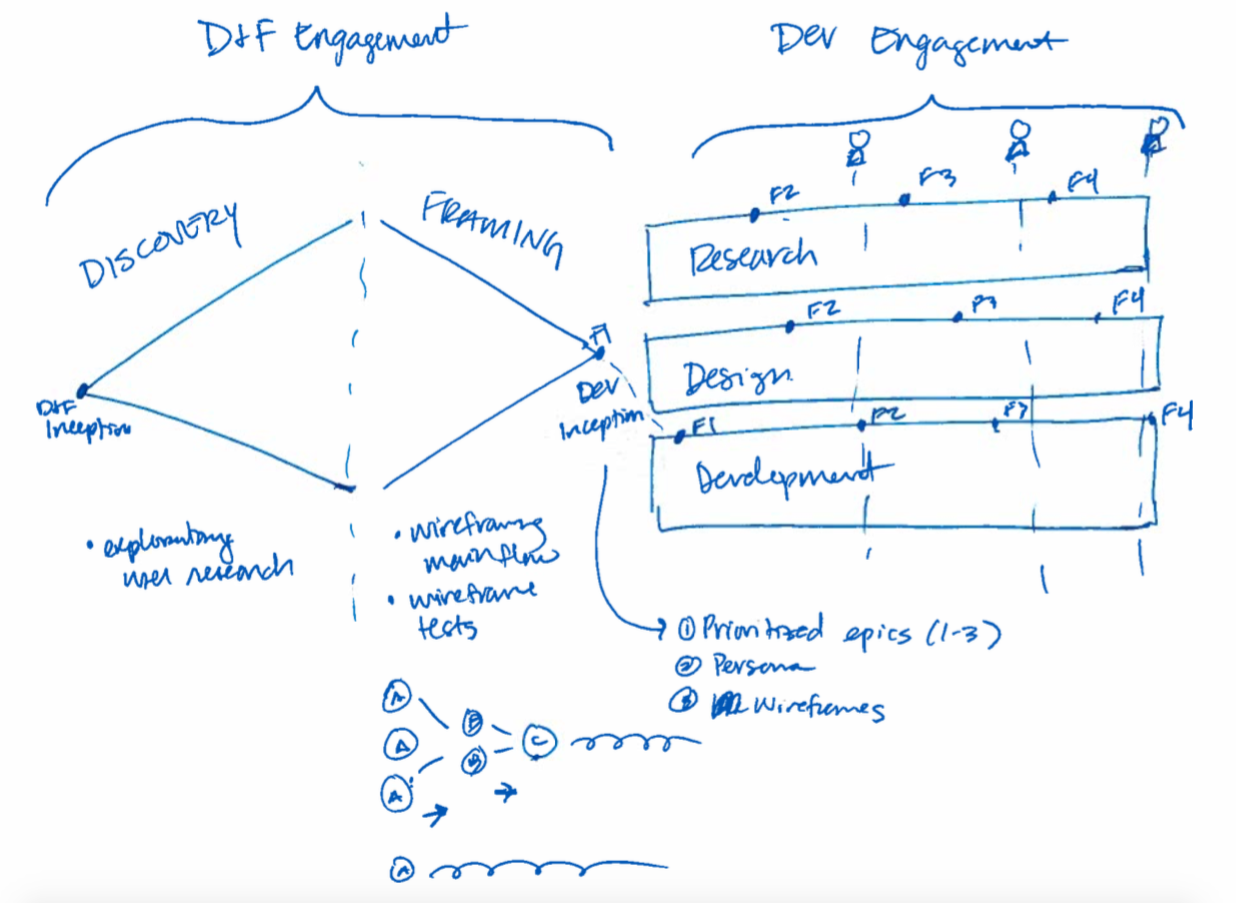
\includegraphics[width=6.5in]{interviews/drawings/2015_05_29.png}
\caption{\quotes{2015-05-29's drawing of a project work flow}}
\label{2015_05_29}
\end{figure}

\textbf{Interviewee:} Does it matter if there's a DNF first or...? 02:39

\textbf{Todd:} However you want it. Typical, ideal, however you want to draw it. 02:44

\textbf{Interviewee:} We actually show this to clients. We have this drawing here. 02:54

\textbf{Interviewee:} Most of the projects that I've been on start with the DNF. We'll call this DNF. 03:07

\textbf{Interviewee:} It's assuming the project has design in development going. This kind of, like, inception. 03:27

\textbf{Interviewee:} And this is dev inception. 03:32

\textbf{Interviewee:} This is your discovery, and framing. 03:50

\textbf{Interviewee:} Here in this area, we're sort of doing more exploratory research and sort of going wide trying to understand the users. That's something we do at the beginning of every project especially if the client doesn't know who their user is or they have ideas of who they are but it's not validated. 04:10

\textbf{Todd:} 	That's the discovery phase. 04:11

\textbf{Interviewee:} Yes. So, this is like exploratory user research. That's like interviews and maybe on site, shadowing people and things like that. And once we have a good idea of who they are, we start wire framing, maybe like the main flow and doing some wire frame tests like user research, that kind of thing and that's kind of within that, I think, we're kind of iterating as well. 04:45

\textbf{Interviewee:} I guess you can either start with one and iterate on that or you can start with many and narrow down. We've done both. So, when you start with many, you just- So, this is like your different As, research, then research to get to C. That makes sense? 05:10

\textbf{Todd:} It's like a portfolio of ideas? 05:14

\textbf{Interviewee:} Yes. I did it on my first project and it worked out really well and then from there you're kind of iterating on what you've come up with. 05:25

\textbf{Interviewee:} We came up with a couple, different nuance ways of doing something because they all seem good and they're like, two or three different features and we sort of combined them in different ways and then we took our insights from that and narrowed it down two versions, narrowed it down to one version. 05:46

\textbf{Interviewee:} I've also done it where you just start with A and you just iterate. I think both worked but this is fun to do. By the time we get to dev inception, we have prioritized epics. You have a develop persona. And you have wire frames. That's kind of the ideal for this point. At that point, development can start on say feature one and in the meantime, we'll start researching feature two. Then, we'll develop it. Then, feature three. So, it kind of goes like that. 06:37

\textbf{Todd:} Nice. 06:39

\textbf{Interviewee:} Maybe you have feature one here and then we'll go here. While they're doing that, we'll start on the next thing. So, on the next thing it flows down. I hate saying waterfall because I know it's the wrong kind. It's like a different kind of waterfall but it iterates in that way. So, we're like, \quotes{Oh, it's going in the cycle.} At any time, we're going to bring in users to test whatever we want. 07:09

\textbf{Todd:} You're drawing people. 07:12

\textbf{Interviewee:} Yes. These are users. At any given point, we can even do exploratory research. We can do wire frame or visual research or we can show them an actual prototype. 	It's kind of nice because you can, whenever you need people, whenever you're stuck on something, you don't have to wait for the right time to bring people in. 	It's just you can test anything at any given time.  07:34

\section{Interview 6 Abridged Transcript with Anchor }

\begin{figure}[h]
\centering
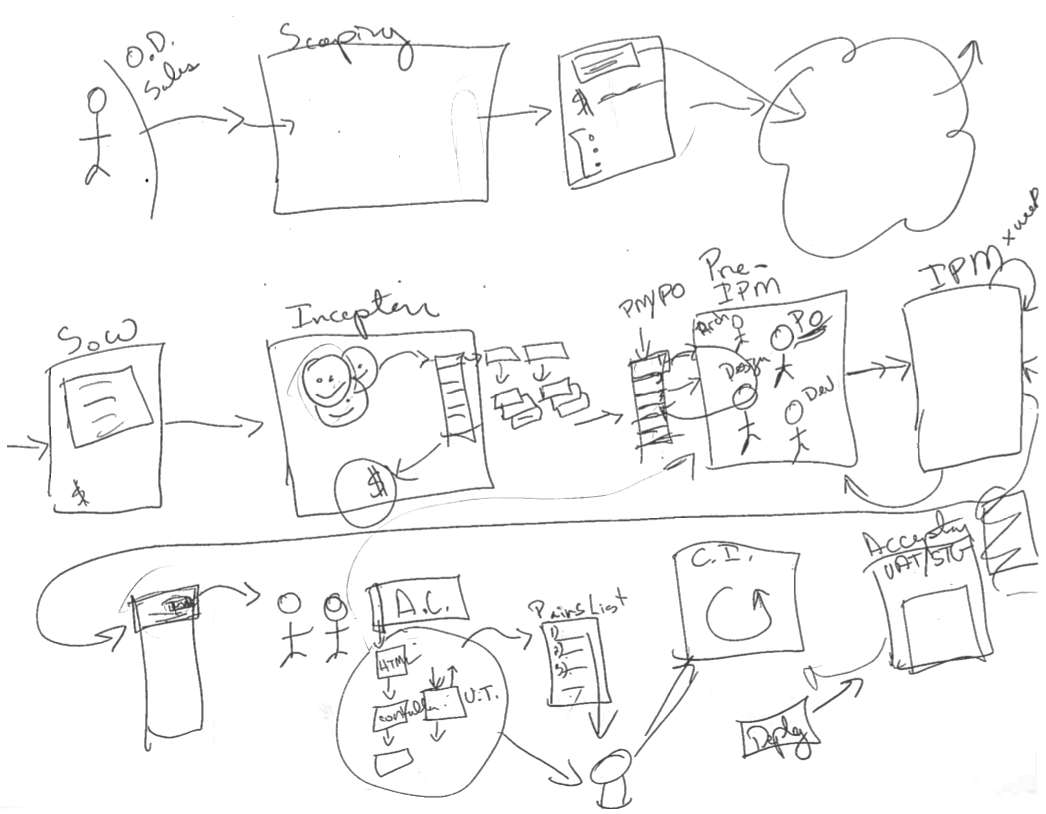
\includegraphics[width=6.5in]{interviews/drawings/2015_08_12_anchor.png}
\caption{\quotes{2015-08-12 Anchor's drawing of software development process}}
\label{2015_08_12_anchor}
\end{figure}

\textbf{Todd:} So on this sheet of paper, could you draw your perspective on our process for software development. 0:00:09

\textbf{Interviewee:}  Our process for software development.  Where do you want to begin?  Or is that like \ldots 0:00:14

\textbf{Todd:} It's a really open-ended question.  0:00:15

\textbf{Interviewee:}  	So there's a customer, a potential customer.  And they come and there's some kind of vetting to, at least, get them in the door.  We think that they have interesting idea of some kind, and maybe we ask a couple of questions; so this might be the OD or sales.  Just some minimal vetting and then just enough for them to say: \quotes{you know what, I think we could possibly have a conversation about what it is that you want to have built.}  So then we do a scoping with them, and in that scoping, the input is their general idea.  Usually, it's like pretty vague; It could be from very vague to they totally know what they're talking about both on their problem space and with the solution to look like.  So then the output of that is a document that basically tells them this is what it likely is, and this is how much it's gonna cost, roughly speaking, and these are gonna be the roles and responsibilities, this is what you would be buying.  What just really actually, some amount of hours of some amount of people, different skill, that's what we're actually promising and we'll aim for this thing, but we'll always constantly trying to give you the best value thing as we go along.  So that's some kind of proposal, I don't know exactly what we call that, but it is all part of the scoping.  0:02:00

\textbf{Interviewee:}   And then, I'm gonna draw, like, maybe a number of stops here; by the time I see it, somebody signed, like, an SOW or similar that was possibly, like, but influenced by that scoping value but who knows what negotiations or whatever happened after that; and probably informed by that document, like, what we say we're aiming to deliver.  But this is, I think, this is more like a legal document or as the SOW is more like a legal document whereas the thing that came out of scoping is more of like a \quotes{come work with us} and some of the other stuff around that.  So then, we go into an all of these assumes it's ok.  I'm talking happy path.  Cool?  0:02:59

\textbf{Todd:}  	Yeah, I'm good.  0:03:00

\textbf{Interviewee:}  	So then we do an inception, and this is where, regardless of what we said over here, we get them to get really clear about who is the person that they're targeting; like, ok so it's about a product market fit, who's the market, what's the product gonna be.  So here's this person or persons or personas, and then for each of one those, like, what are the kinds of things that they need to get done, right?  So they've got things that need to happen, that ultimately will result in to some kind of outcomes, and it almost always like it's gonna convert to dollars in some way, shape, or form.  Sometimes it's a non-profit thing and that's slightly different, there's mixed motivation.  So then what we do is we say, \quotes{ok, in order to meet those tasks, what we need is features from the product} and so we're calling out, like, epics, if you will, feature sets, whatever, and then when we start breaking those down into individual stories and these are just sketches at this point.  We're not gonna get all into acceptance criteria right away, it's just like trying to enumerate coz really the outcome of the inception is a backlog. 0:04:43

\textbf{Interviewee:} So you've got some product owner, who culls the outcome of that into a prioritized list of stories, each one of those describes at tiny interaction between this person and the software that we're building.  Ideally, there's variations on that but then, so that's what an individual user story is.  0:04:58

\textbf{Interviewee:}   And then we go to kick off.  So then, we have our first iteration planning meeting where we take as input the prioritized backlog and for each story we go through them.  And by then, the product owner has got them into a point where I call it readied, they've met the definition of ready, which is they have clear acceptance criteria.  There might even be, a pre-IPM where that work is done, as well as, so this is the input is the backlog and the output is the backlog in the pre-IPM.  There are two things that happen, one is that we get clarity early on what the requirement is, and the other is that we get technical input to help with that prioritization and viability, like, \quotes{ok this may seem simple, like on the face of it}, but actually, there's a whole of things that has to happen to make that work, etc. So we surface some of that, the pre-IPM includes somebody from the product side of the house and someone from development, so product owner, development.  Sometimes depending on those, the story can get more complicated, the more requirements, with the greater the variety or the more exotic the product is.  So you might even need someone in from design who is kind of help guiding how this should unfold and the interactions between things because there's all kinds of decisions from that end.  I Imagine, although, we haven't done this yet, in an enterprise client that you might even have somebody from like architecture there, business architecture.  The point of this conversation is to get all of the perspectives that need to be folded into the prioritization and the validation of, that the stories are legit.  0:07:11

\textbf{Todd:}  	Yes.  0:07:12

\textbf{Interviewee:}  	So then that goes into IPM, and this is a straight-forward roll through - the from top to bottom - the backlog, and we go over each story.  We read out title, we read through the acceptance criteria and then the team points each of the stories, the purpose of that is to surface complexity and to get a general, like, understanding, like, common understanding of what this thing actually is, what it is, what's gonna be involved to building it.  0:07:52

\textbf{Todd:}  	Yes.  0:07:53

\textbf{Interviewee:}   	We don't give in to like, we try not to give in to implementation details.  Sometimes, we have to dip down for a second to like verify that we're all speaking the same language, that we're all really envisioning the same kind of thing.  But that usually is surfaced by like, \quotes{I pointed at one and you pointed at five,} and then I would like \quotes{what?}  So then that hopefully prompts a conversation.  If we all said three, it's good enough for now we move on, if we all think it's about the same thing and the product owner doesn't lose their mind hearing that number, then we're all kind of okay.  Then the output of the IPM is individual points on the stories, and we typically go for some amount of horizon so the minimum that I feel comfortable walking out with is at least for the week, so we don't have to, like, break the flow of getting work done before the next IPM because we're gonna do this once a week, these IPMs we're gonna do this once every week. But ideally, a little bit more runway so that we mitigate against that the team haven't jumped out of the flow and also to, like, help the product owner have some room to sort of steer.  If they only have so many points in the stories, then they have to kind of pay the price of reprioritizing. So that's IPM.  Haven't have written a line of code yet.   So then, after IPM, we get working. So out of the backlog, a pair picks up a story and so then that pair looks at the story...  How deep do you want me to go, because I can go all the way down to like testing and stuff.  0:09:48

\textbf{Todd:}  	Sure.  0:09:49

\textbf{Interviewee:}	Ok.  0:09:50

\textbf{Todd:}	This is your diagram.  There's no wrong answer.  0:09:54

\textbf{Interviewee:}  	Alright. Ok.  So, the pair looks at the acceptance criteria and they say, \quotes{hmmm.... what test do I need to write that will help?  Or a set of test that will help if those tests ran green?  I feel really confident that we've met the spirit of that story.}  So they start there.  Usually at pivotal will do typically outside in so that means if we write something that looks like an acceptance test, something that describes very closely what this person with the persona experiences both in what they do, and what they see back from the software.  So we write the starts, we start with a very low fidelity version of that. It's not gonna describe the whole interaction, it might describe the smallest piece of we could possibly articulate; so we start there.  And then we run that test and it fails.  Then we say, \quotes{hmmm, ok, so we're in this architecture, what's the next part that we need to build in order to begin to meet those needs?}  And we work our way down the architecture.  In a typical web app, there's something that's displaying, an HTML page, and then there's something that is probably orchestrating the generation of that HTML, like a controller and usually we try and separate our concerns. We think about these things as we work our way down driven by trying to meet just this one acceptance test.  0:11:26

\textbf{Interviewee:} So along the way what we do is we write individual unit test for the components that have interesting behavior.  The controller does have interesting behavior.  It takes in some input and it makes some decision about what should be the output, what should be the resulting HTML.  And that controller also interacts with other collaborators.  So we have tests that say, are you properly handing off these parameters?  So these really fine-grain unit tests. But the key is that these things are, each time we write these tests, we're setting an expectation on that little tiny piece of the system, in the same way that our acceptance criteria are setting an expectation on the software, and our user stories are setting expectations on the feature .  So forth, all the way back up. We're trying to be needs-based  all the way down as we do this; that's probably good enough.  The details of how that happens varies wildly and even like within this, there are different schools of thought about how that happens.  There's people who believe in writing units for every little thing and people who say \quotes{no, you can set certain bullwarks} and write tests around the bullwarks.  Let everything sort of float in between.  0:12:43
\section{Interview 7 Abridged Transcript with Product Manager }

\begin{figure}[h]
\centering
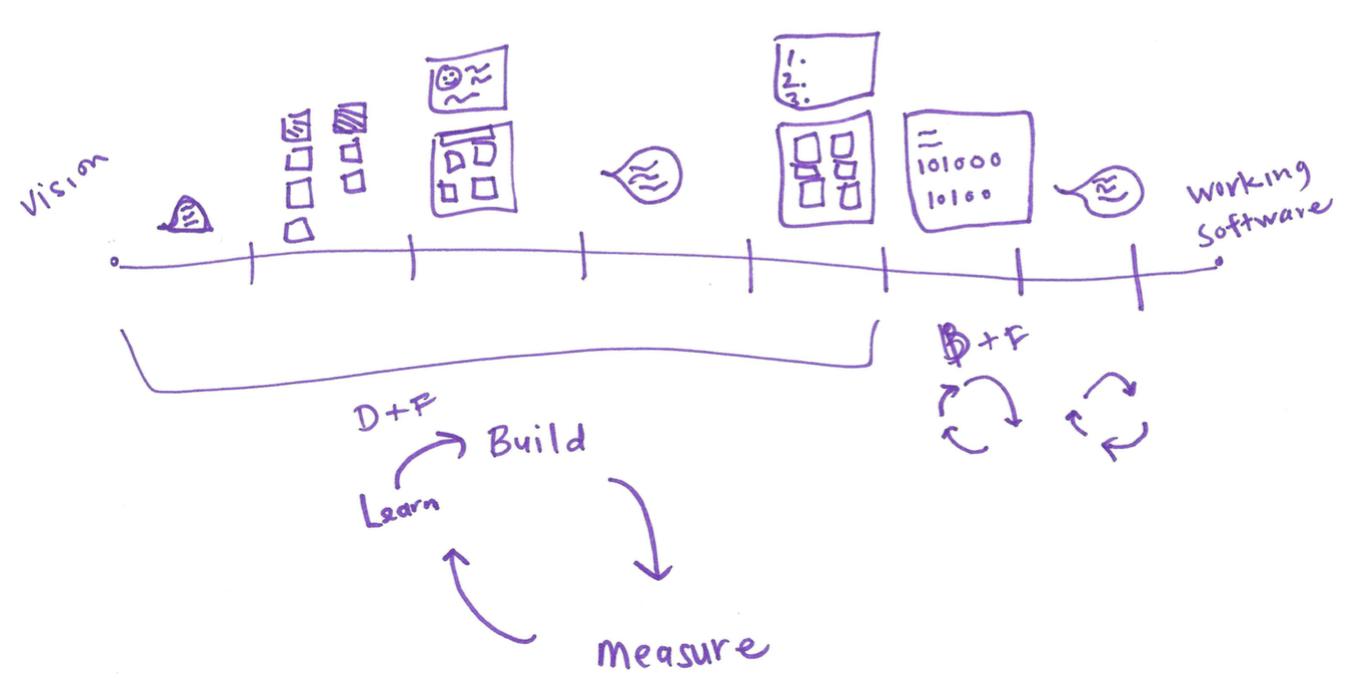
\includegraphics[width=6.5in]{interviews/drawings/2015_08_12_pm.png}
\caption{\quotes{2015-08-12 Product Manager's drawing of software development process}}
\label{2015_08_12_pm}
\end{figure}


\textbf{Todd:} If you're open to it, could you, on that sheet of paper, draw out how you view the way we build software? This is completely open-ended. There's no wrong answers. And just take a stab at it.  0:00:21

\textbf{Interviewee:} So I'm drawing a line, it's like product on a continuum. We're gonna have vision here. We're gonna have working. Can you tell I'm a PM because I'm writing in lines, boxes can't do? 0:00:45

\textbf{Todd:} I love it.  0:00:46

\textbf{Interviewee:} So let's see here. So let's do a couple of lines here. Alright, so let's say, each of these represents two weeks.  So we'll say that the first point, so how we build it at pivotal is that what you asked?  0:01:17

\textbf{Todd:} Yes.  0:01:18

\textbf{Interviewee:} So it starts with having clients.  0:01:20

\textbf{Todd:} How would you build it too?  0:01:21

\textbf{Interviewee:} Yeah, yeah. Totally. The reason I asked about Pivotal is 'cause we're doing consulting. So if you're thinking of product as a continuum, our clients come in in all these different ways of where they the insert. But it starts with a conversation, kind of like a qualifying conversation of like, \quotes{hey, what do you wanna build?}, and \quotes{what's the fidelity of your idea?} And from there, we have a good understanding of if they're at a stage where they can build something, or if they maybe really need to think about it further.  But once we realize ok, they're ready for Pivotal , we'll start with a Discovery and Framing and not every project gets Discovery and Framings, but in the LA office, a lot of them do.  We're trying to get most projects getting some a semblance of Discovery and Framing.   0:02:04

\textbf{Todd:} When would you not do one?  0:02:07

\textbf{Interviewee:} So we won't do one... I think we can make the case really for all projects could do with a little bit of DNF right? So even if you're like, I know where to build from. So with FYI rather, but for a PM, I'm thinking, okay my role is to help the client understand who are we building for and then what we are building and when? So for the, who are we building for, I think all clients.  It'd be great if we could do some user research with them even if they are like, we did all these user research just to do a quick gut check, like hey this makes sense, that'll be great.   0:02:42

\textbf{Interviewee:} But I think a lot of the times when we don't do them, it tends to be convincing the client or if there's a budget concern.  So they have enough of a fidelity of understanding who their target user is and who the secondary users are and have a persona and are focused on stuff like kinda key factors, ok, if you're saying you want to build an app for the millennials and for college-age students and for the ages 25-35, that's pretty vague.  We do get that a lot, but we're saying, \quotes{ok, it's for millennials, so what gender are we going for?} Or is it, \quotes{what are their behaviors like?}  There's a lot of questions that we can ask on this conversation. and these qualifying calls to say, to kind of fish out, to think if they are ready to work with Pivotal, or if they have enough information for DNF or not. So, does that answer?  I guess that was a very specific answer.  0:03:44

\textbf{Todd:} That was great.  0:03:46

\textbf{Todd:} I interrupted your flow.  0:03:48

\textbf{Interviewee:} No, no, this is fine.  So I'm of the opinion that I would love it if we could have some sort of research with all of our clients and users. Typically when we do a DNF, Discovery and Framing, we do that for 4 weeks on average, sometimes it's up to 6 weeks depending on how many users they have and how many people they want us to focus on.  But we typically really try to work on 2 to 3 target users being 1 primary user and maybe 2 users of the system that kind of insert in their day.  And then we've done a 2 week of design first or Discovery and Framing but really it's just \quotes{let's talk to some users and validate some ideas.} But the whole goal of this Discovery and Framing process is to do a couple of weeks of talking to users, of about 2 weeks and that's when we're doing some of those exploratory interviews, kinda turn it into elicit narratives to understand what their behaviors and what their days are like.   0:04:51

\textbf{Interviewee:} And then from there, we can isolate what are some of their pain points and what are some of the frictions and inefficiencies and how are they capturing data and what are the tools that they use and who are the people they're talking to.  From there, I guess one thing I didn't mention which is important is to say, what are the product goals that our clients have?  And what are some of the assumptions that they have about their products?  About their users where their products can help solve their needs.  We go into user research, alright, here are some assumptions, hypothesis that we have, let's test them. Out of that output of user research is that we have this, we do some synthesis and analysis of all of the things they're talking about.  We record the things that we saw, so if they're in a cubicle and they have tons of printed out papers because what they do is they get stuff by mail and then they have to scan it in.  Those are the things that we're seeing that are part of their day that can affect them.   0:05:54

\textbf{Interviewee:} What did we hear, like things that they're telling us about their day, and things like we felt that they're telling us. But maybe there are some subtext and some nuance there saying everything's great but their faces are really strained and you can tell they're really frustrated and their posture has changed when they're talking about certain subjects. Kind of taking all of the things that recording from our user sessions and then coding it by what we saw, what we heard, what we felt and then finding themes. What are users talking about? Usually when we do research, we try to do 3 to 5 users, so that way we have a good cross-sample and in case there's any extreme people that we meet, it kind of helps us give a better analysis, better data sample. So we'll kind of call all the information that we have and we'll go to them, too.  So we'll go to their cubicles or wherever their workspaces are. So we want to get a sense of their environment. Cause there's so much contextual information there that you can't get just from having a phone call with someone.  0:07:02

\textbf{Todd:} Yes.  0:07:03

\textbf{Interviewee:} So, then, that's usually about a couple of weeks doing some researching.  As we're doing the researching, we're capturing all of our information on notepads and then we're doing what we call infinity mapping, affinity mapping.  We'll get one of those big foam cork white boards and we'll take a listen to the recordings of when we're doing user research or if we can't record just looking at our notes because our notes are like, you're almost writing verbatim what people are saying. Because you don't want to put all your analysis in there at this point, you just want to get them to talk and get it all in, and then we'll take each kind of idea and we'll put it on a post-it note and we'll have a bunch of post-it notes around and they'll be coded by what we saw, what we heard, what we felt, and then we'll start seeing themes around this post-it notes.   0:07:54

\textbf{Interviewee:} So there's this one user that said there is a lot of things around education and tools and timeline and whatever it is.  Then we started noticing trends, so we'll start taking those nuggets and we put them across this themes and then we'll do that to all our users; and then from there, we'll do another round of synthesis and the ideas are going to keep condensing.  So then we have a synthesis of all the people we talk to and what the overlaps are and the themes of what their day is like, and the behaviors they drawn during that day.  And then after that, we'll map out their day, like what are the tasks that they're doing, and then map out from the tasks all those insights rather not insights but nuggets of what we heard from them, that we kind of collectively called down and condensed and we'll put those against the tasks.    0:08:43

\textbf{Interviewee:} So when they need to schedule a user for an event, these are all the things they said about it, or these are the things we saw and the things that we felt.  So then what's cool about that is we do that for every target user and you can map them out.  So you say 'here are three target users, here are their days and here are all the intersections of their days'.   So you can tell visually, \quotes{oh, you know what, when this person does something, you notice the next thing, these two people are affected.} And then you can start isolating pain points and inefficiencies and you get these really nice overlay of what the system, not the digital system but just the users in the workplace and what their days look like.  So when I'm mapping out the process, I'm thinking of conversations, that's a little talk bubble.  0:09:43

\textbf{Todd:} Ok, I like it.  0:09:44

\textbf{Interviewee:} And then I'm having doing some synthesis. Someone do a little post-it map.  0:09:51

\textbf{Todd:} Ooh, I see the post-its.  0:09:53

\textbf{Interviewee:} There you go.  And then from that, we say, \quotes{ok, based on our research, this is what we say a persona or what this user looks like.}  We think of \quotes{what do they need? What are the tasks in their day and what do we need.} So we pull out insights from that. This user really has trouble communicating with the other people on this team because they don't have the right communication tools setup or whatever that is. They need a better communication system.  Once we have these needs, and bits and insights of who they are and what they need, then we can say, \quotes{all right, how can our products solve these needs?} Then we say, \quotes{we have some product ideas based on what their needs are, let's validate them.}   0:10:55

\textbf{Interviewee:} Then we'll go back and talk to the users. We'll drop some wireframes and say, \quotes{all right, based on what you guys had said, we feel that here's a quick prototype, clickable prototype} And we'll use invision.  We'll say, \quotes{Why don't you click around? What do you think about these things?} we'll do some user testing there.  And then from that information, we'll further validate or dis-validate our product ideas and we'll do another product evolution but kind of the output of this 4 week on average DNF cycle as that you'll have Wireframes and then you'll have some personas. You'll know who your end user is.  You'll have empathy drawn for your end user which is the whole goal. You'll have a problem that's been framed and validated.   0:11:38

\textbf{Interviewee:} So that way, it really de-risks development cause it's pretty great to come in to development and we know that when we're making product decisions, we can go back to this research.  We're like, \quotes{oh, if we're going to do this or this, then what do they actually need? What was that they talked about that really indicated this is the right approach?} It also helps us speak a language that our users speak.  Which is really important for the development team but all the other stakeholders involved in the process.  0:12:05

\textbf{Interviewee:} Words are everything, right? So we want people to be kind of on the same communication levels of talking how their users would talk, so that way it helps us draw all that empathy throughout the entire development process because you still need to draw on that, you know 6 weeks, 3 months, however long into the development cycle until you're releasing. Right to be able to have that insight of what they want. I think the cycle is... Let's just say that you've done some analysis and you've done some wireframing, and then after that, we'll talk to users again.  After that, we'll do another set of wireframes. We'll also do some persona mapping here as well as making these wireframes.  And then after we do that, we will create a feature list.  0:13:13

\textbf{Todd:} Yes.  0:13:14

\textbf{Interviewee:} We'll say,  we're not gonna\ldots  What could the next you know 2 to 3 kind of epic areas. We'll say, let's give some insights here.  Maybe, we have 3 insights and 3 needs.  Let's do 3 feature ideas and how do these feature ideas map these needs?  So we write these feature ideas and we'll say, down in the documents and user needs this and we'll help them achieve their goals.  Business needs this and this will help them achieve their goals.  We're always aligning user business needs throughout the entire process. So then when we get into development, we'll just make a little terminal, I wish I had multiple colors.  0:14:00

\textbf{Todd:} Next time, you'll have to bring your can.  0:14:03

\textbf{Interviewee:} So, when you're getting into the computer, when you're getting into development, you're able to have a backlog that's been built.  You have the first couple of weeks of features.   0:14:17

\textbf{Todd:} Yes.  0:14:18

\textbf{Interviewee:} You have some ideas and you start building and then once you release something, which could be in a week or could be a couple of weeks depending on what you're doing.  But once you get into the first bit of business value working software, then you can go and you could talk to your users again and then you learn from them and then you continue on.  So at that point, what you're doing is you're building something and then you're measuring it.    0:14:45

\textbf{Todd:} Yes.   0:14:46

\textbf{Interviewee:} And then you're learning from it right?   0:14:48

\textbf{Todd:} Uh-huh. Yes.  0:14:50

\textbf{Interviewee:} And then you're going back to building, right? So that's what we're doing for this whole process. So the feedback loop is really important. When I'm thinking about the extent, the depth of all this research, then you don't need to have a DNF to do any of these research.  You don't have to sell that in, you can do...  So the training that our designers and our PMs have, and now we're trying to have our developers be exposed to it, as well.  To say, \quotes{ok, developer, you get a client project. Development starts tomorrow, you can still talk to some users.  You can still setup user testing.}  And you can do that throughout the entire process.  So it's almost like this whole upfront part, with the DNF.  You're making little DNFs through it, right?  So whoops, it's really you're taking this and you're kind of doing a DNF cycle.   0:15:42

\textbf{Todd:} Yeah.   0:15:43

\textbf{Interviewee:} Whoops, and you're doing that here, and then you're going to do it again. So each week, you might be bi-weekly.   And that is ideal, right?  But sometimes you don't get the users?  So there's a lot of, kind of…  You have to be pretty scrappy with how you do this sometimes, you don't just get this nice set of users at your disposal, you know; but it's so important and I think that's something we do a good job with is convincing our clients, we wanna de-risk this for you so this is how we can do it.  I mean go, it makes sense.  It's very practical stuff.  It's not rocket science honestly.   0:16:20

\section{Interview 15 Abridged Transcript with Interaction Designer }

\begin{figure}[h]
\centering
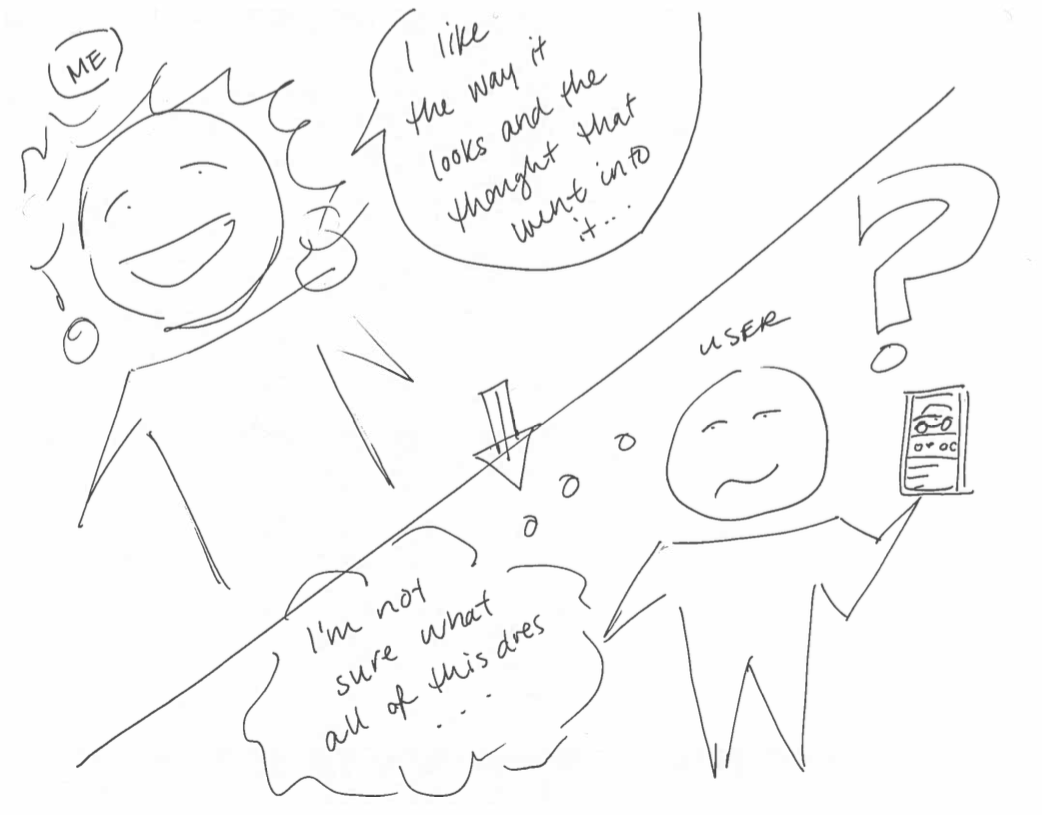
\includegraphics[width=6.5in]{interviews/drawings/2016_01_08.png}
\caption{\quotes{2016-01-08 Interaction Designer's drawing of software development process}}
\label{2016_01_08}
\end{figure}

\textbf{Todd:} My first question for you is very open ended.  00:02

\textbf{Interviewee:} Okay.  00:03

\textbf{Todd:} There is no wrong answer.  I was hoping if you could draw how you feel about the product.  00:09

\textbf{Interviewee:} Okay.  This may get elaborate.  00:27

\textbf{Todd:} Fantastic.  00:29

\textbf{Interviewee:} This is my new pen so.  [Pause] Here we are.  I did sort of a story board-ish type of thing.  02:54

\textbf{Todd:} I love it.  02:55

\textbf{Interviewee:} So, do you want me to explain it?  02:58

\textbf{Todd:} Please.  02:58

\textbf{Interviewee:} Okay.  On one hand superficially, I'm happy because aesthetically, I think it's nice.  I think it's, when you compare it to some of the projects we do, it's been going on for so long and there's such a huge team of smart people.  I feel like we got so much done and it's complex and interesting and there's lot of thought that went into it and it's a really robust app but I'm worried that even though it's pretty and we built a lot of features and the technology is cool, not all of it is necessarily useful for end users and I didn't even give the user name anything because I don't even know that we're designing for the right person all the time with some of our features.  I don't know.  So, I'm worried there were will be more confusion in the marketplace than I would like there to be in a product that I've worked on.  03:57

\textbf{Todd:} Anything else?  04:01

\textbf{Interviewee:} In the drawing or in general?  04:05

\textbf{Todd:} Both.  04:06

\textbf{Interviewee:} Not so much in the drawing.  I guess the big question mark is just that I don't know, I think it's pretty usable but I'm worried there's going to be features for the users or going to be like what is this or why do I care or they'll have question marks around there's something really obvious to me like \ldots I would like you heard a lot of feedback, I want a light telling me if my oil is low and that's just not something we could do because of constraints on the technology I think.  So, I'm worried if people will look at it and say why is there all this stuff that I don't want and there's some stuff that maybe feels really obvious to some users that we haven't provided for one reason or another but overall, I still feel happy.  I think we created a solid product.  04:59

\textbf{Todd:} Good.  When you were describing your \quotes{you} picture, you used the word \quotes{superficially}.  I don't remember the exact word but something like given this superficially I feel happy about it and I was curious if there was like an under feeling of the product.  05:17

\textbf{Interviewee:} Yeah, currently to some degree, this is the under feeling.  The superficial part is a little bit as a designer is a normal person walking around, you feel like people look at it and like it's so beautiful and that might be the beginning and the end of what they think of the app.  They might not use it.  Maybe, it's not for them.  I feel like I could put it in a portfolio or take some of those App Store screens and show it to people and maybe like oh my God, this is the nicest product, you must have done a great job or your team must have worked really hard but if we built something that's really beautiful but doesn't meet the needs of our users, it's kind of I'm still superficial.  I guess part of me is still happy it's beautiful at least or that there's parts of it that are really pretty but at the end of the day as a designer, it's kind of a big fail to build something that's pretty but not the right thing.  It should be a big fail for everybody but especially as the designer, that's what you want to avoid.  06:21
\section{Draw your view of Pivotal's software development process }

\begin{figure}[H]
\centering
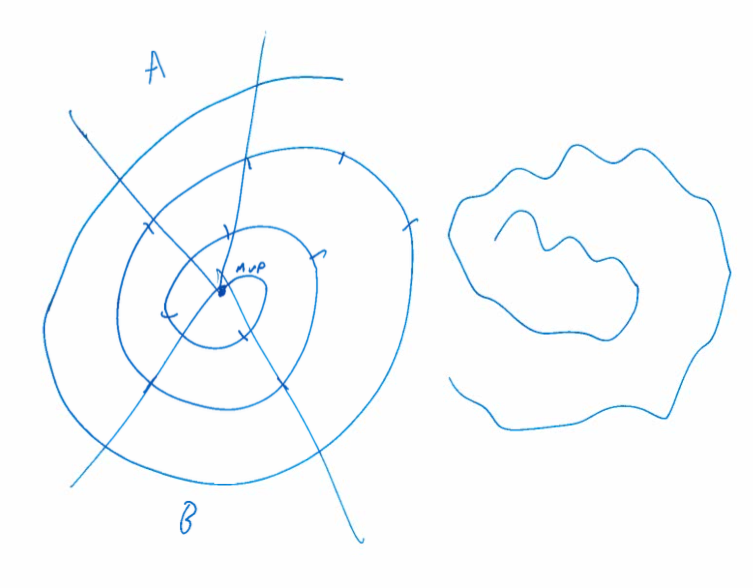
\includegraphics[width=6.5in]{interviews/drawings/2015_06_02.png}
\caption{\quotes{Interview 2: Product Manager's drawing of software development process}}
\end{figure}

\begin{figure}[H]
\centering
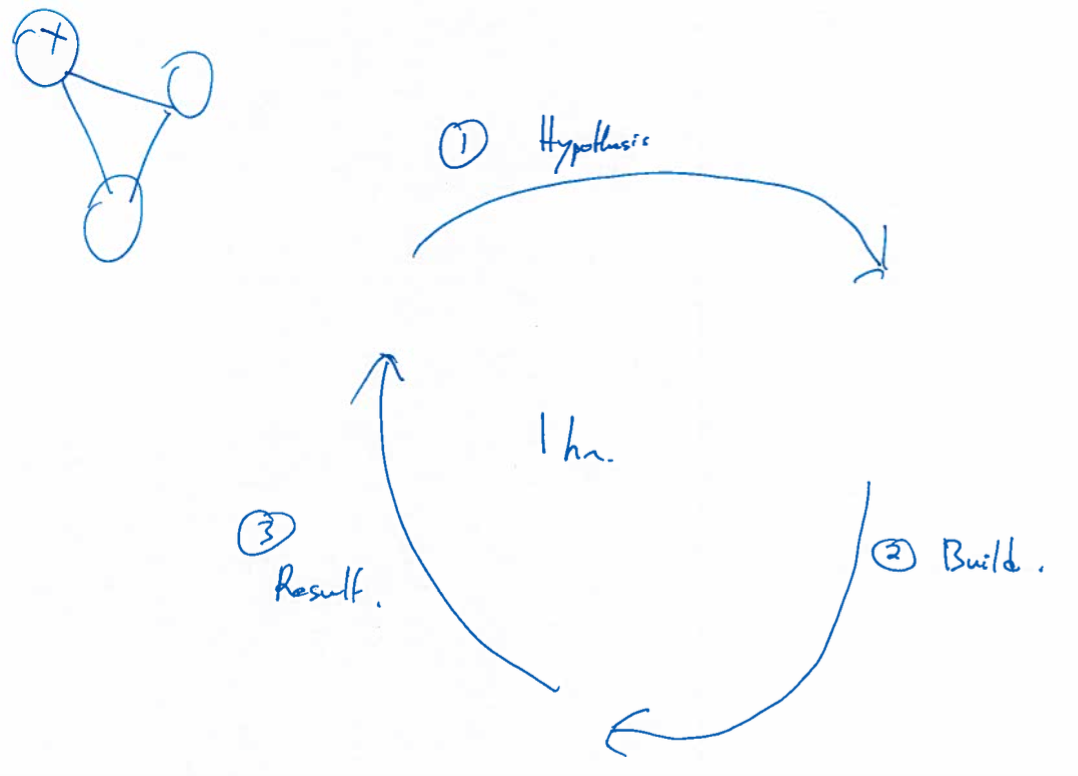
\includegraphics[width=6.5in]{interviews/drawings/2015_06_29a.png}
\caption{\quotes{Interview 3: Product Manager's drawing of software project workflow}}
\end{figure}

\textbf{Interviewee 3:} I try to first come up with some type of hypothesis that I want to test. Then, I'm going to build something that's going to test this, then I'm going to try to get a result. 

% \begin{figure}[H]
% \centering
% 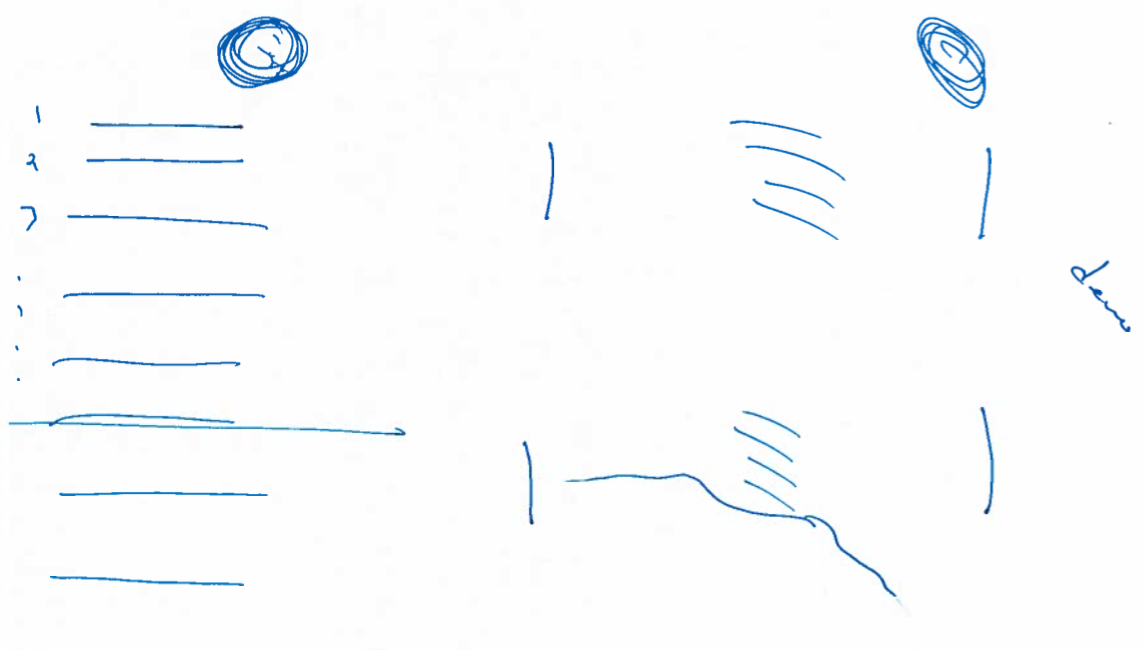
\includegraphics[width=6.5in]{interviews/drawings/2015_06_29b.png}
% \caption{\quotes{Interview 3:  Product Manager's drawing of software development process}}
% \end{figure}

\begin{figure}[H]
\centering
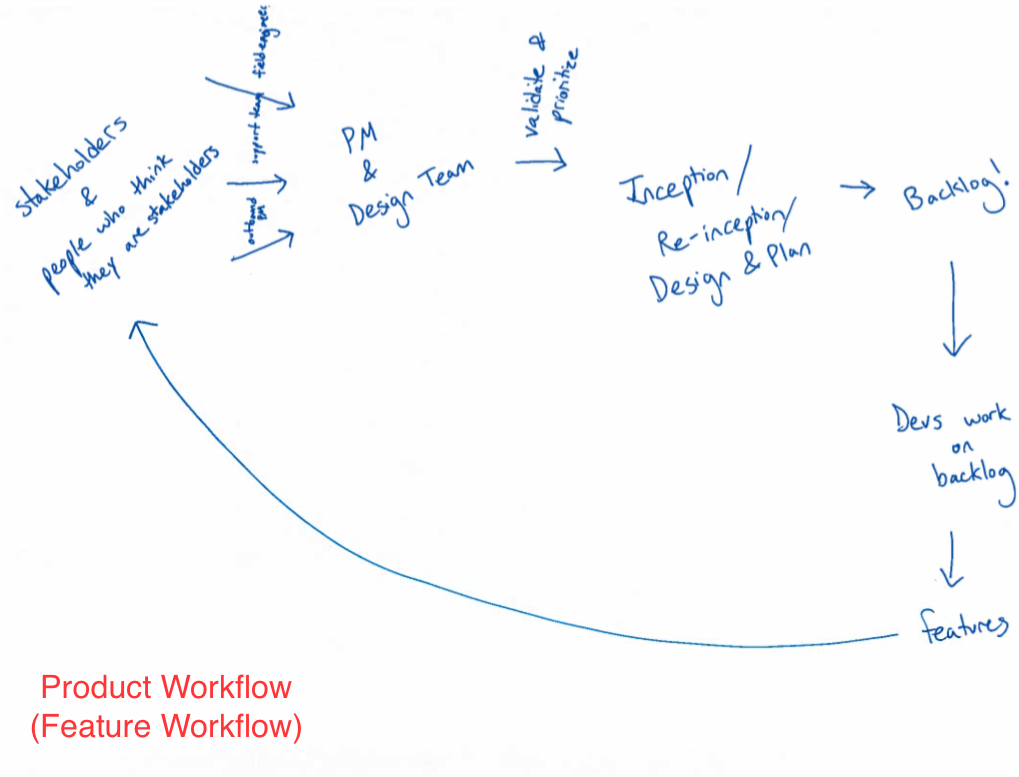
\includegraphics[width=6.5in]{interviews/drawings/2015_07_31a.png}
\caption{\quotes{Interview 5: Product Manager's drawing of software development process}}
\end{figure}

\begin{figure}[H]
\centering
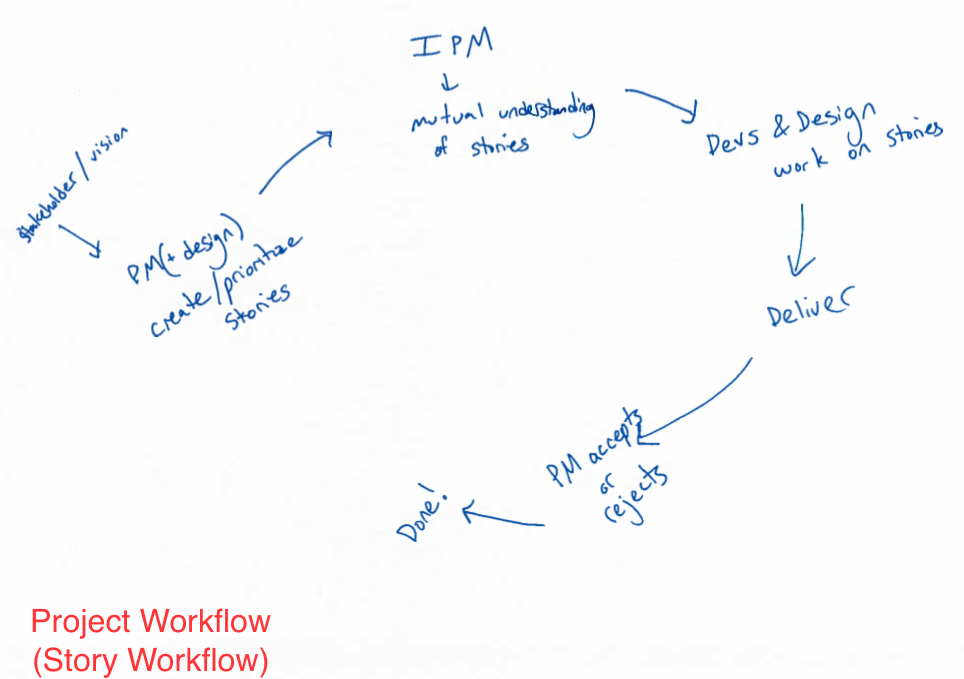
\includegraphics[width=6.5in]{interviews/drawings/2015_07_31b.png}
\caption{\quotes{Interview 5: Product Manager's drawing of software development process}}
\end{figure}

\begin{figure}[H]
\centering
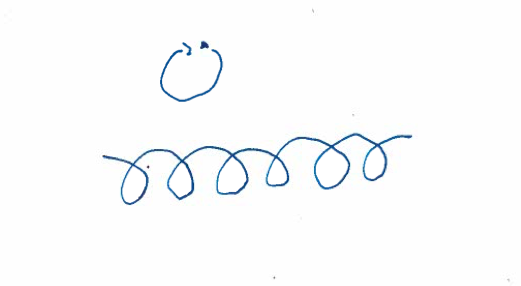
\includegraphics[width=6.5in]{interviews/drawings/2015_08_12_se.png}
\caption{\quotes{Interview 8: Software Engineer's drawing of software development process}}
\end{figure}

\textbf{Interviewee 8:} We iterate on stuff that we have a touch point and we're going to go away and do work and come back to that touch point. To me, it sort of looks more like a spring, you pull the slinky or you have a pig's tail that you stretched out. We are trying to do is orbit this idea of always working with each other. The red, green, refactor is a very tiny cycle that we do. We're trying to setup ourselves up, a check-in point where we can start somewhere and move a little bit and make sure we're okay and come back again and have another starting place and you can do that in 5 minutes with a test. Then you see us play that out at higher level of stories and then higher level again with our daily stand-ups, and higher level again with our retros and our check-ins there and higher level again with our inceptions. It's really about managing the feedback cycle or the check-in points to make sure that we're kind of all fluidly communicating about how we're affecting and doing things. Because the minute we stop communicating, is the minute we start to get off and be in the weeds somewhere.



\begin{figure}[H]
\centering
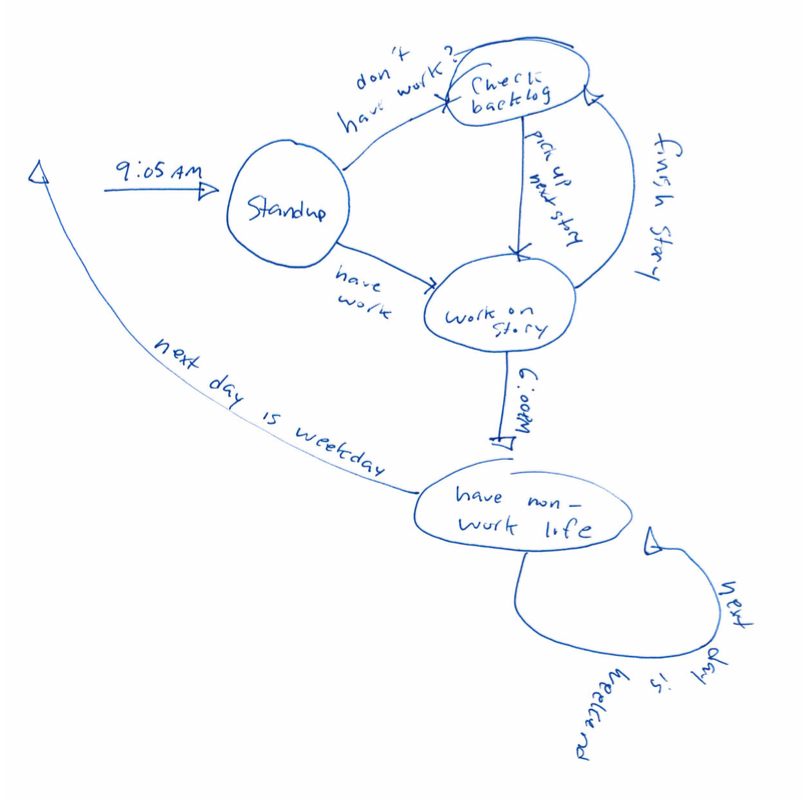
\includegraphics[width=6.5in]{interviews/drawings/2015_09_02.png}
\caption{\quotes{Interview 9: Software Engineer's drawing of project workflow}}
\end{figure}


% \begin{figure}[H]
% \centering
% 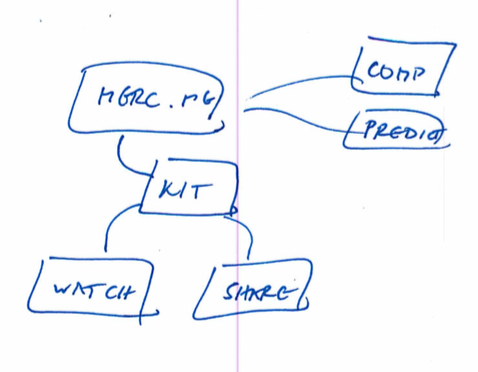
\includegraphics[width=6.5in]{interviews/drawings/2015_12_18a.png}
% \caption{\quotes{Software Engineer's drawing of software development?'}}
% \end{figure}

\begin{figure}[H]
\centering
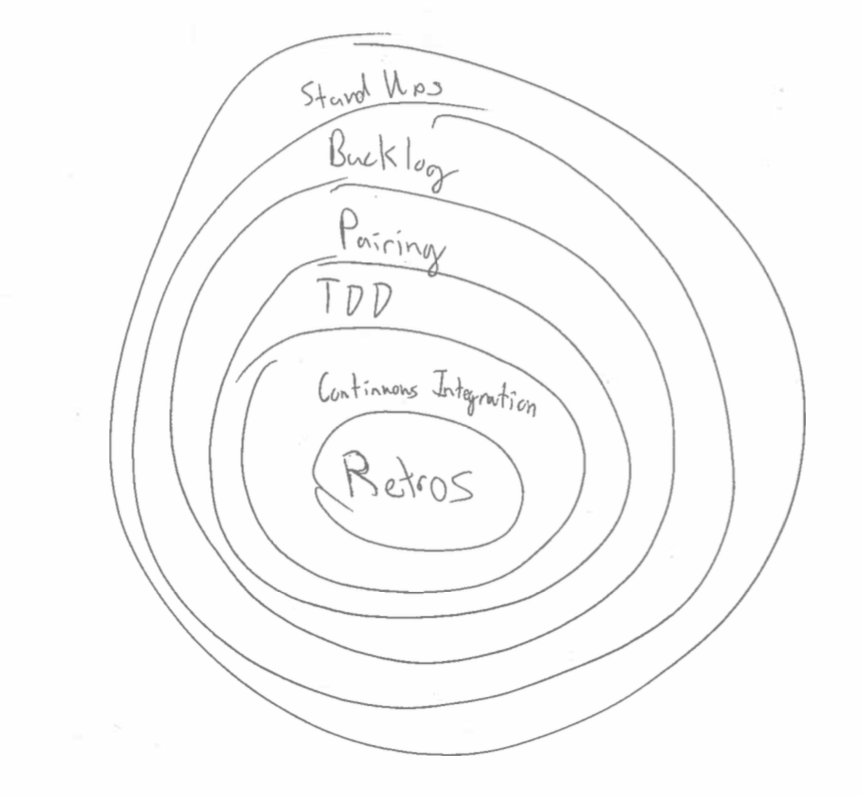
\includegraphics[width=5.5in]{interviews/drawings/2016_01_15.png}
\caption{\quotes{Interview 18: former software engineer's drawing for the Pivotal software development approach}}
\end{figure}

\textbf{Interviewee 18:} [The circles are arranged from an inner core practices to outer rings that are more negotiable.] These are the things I think are core to how Pivotal Labs does software development from the most important.  Basically, if some client wanted to drop things outside of it, this will be the order that I think we'd agree to have it be dropped.  I don't think we'd ever drop retros but I think we might drop the backlog or something that we probably still would.

\section{Draw how you feel about your current product?}

\begin{figure}[H]
\centering
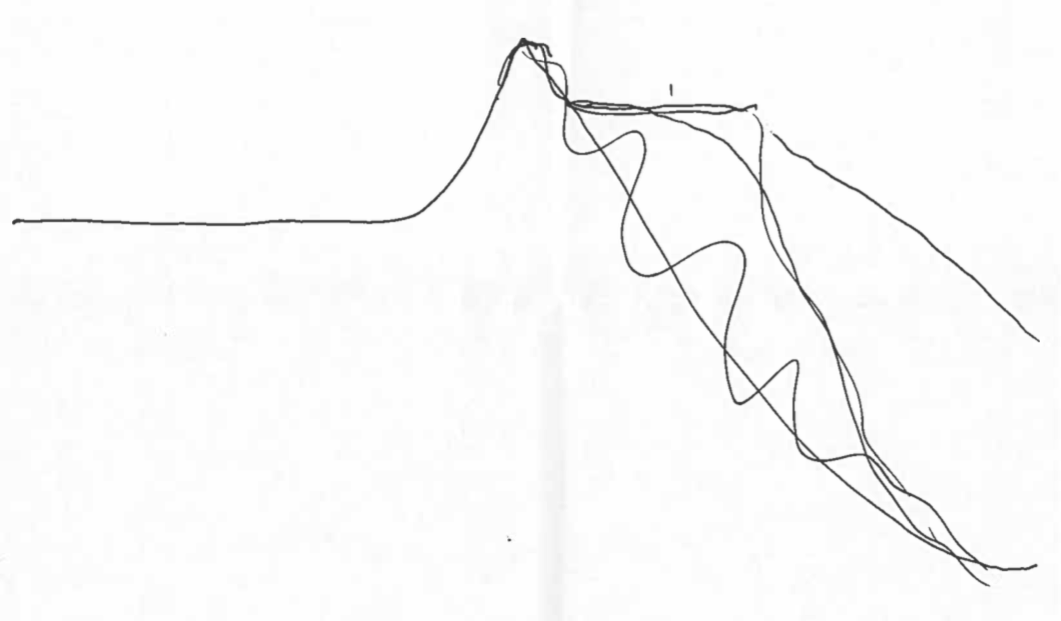
\includegraphics[width=6.5in]{interviews/drawings/2016_01_08_designer2.png}
\caption{\quotes{Interview 16: interaction designer's drawing for `how you feel about your current product?'}}
\end{figure}

\textbf{Interviewee 16:} The peak  was very like a successful moment for Pivotal. It's really cool to see how many people appreciated what we've done. Against all odds, we released this app. I felt proud to be on that team. \ldots 

[The graph goes down] as the design started getting cut. The only thing we're doing is bugs. We designed all these cool features that we're excited about. Almost none of them are getting into the app. It's been almost every week that a feature in the new design is no longer in [the release]. We don't need [what I worked on] anymore.  It feels very frustrating as a designer. I can't affect that that much.

\begin{figure}[H]
\centering
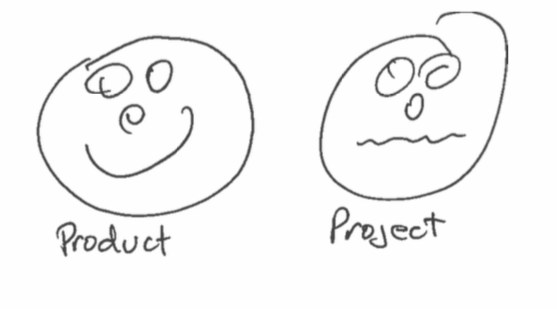
\includegraphics[width=6.5in]{interviews/drawings/2016_02_25.png}
\caption{\quotes{Interview 21: Product Manager's drawing for `how you feel about your current product'}}
\end{figure}

\section{Draw how you feel about the code}
\label{AppendixFeelAboutTheCode}

\begin{figure}[H]
\centering
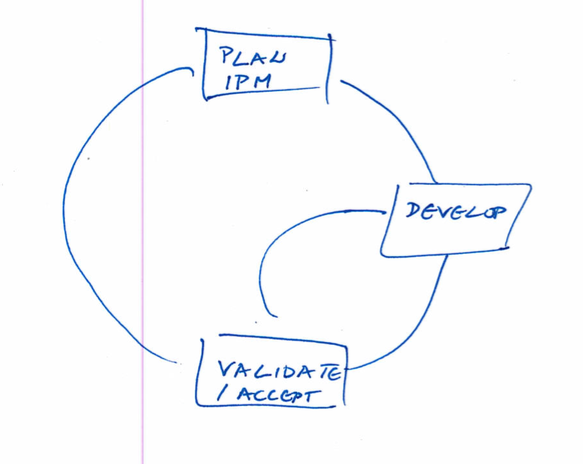
\includegraphics[width=6.5in]{interviews/drawings/2015_12_18b.png}
\caption{\quotes{Interview 14: Software Engineer's drawing for `how do you picture the code?'}}
\end{figure}


\begin{figure}[H]
\centering
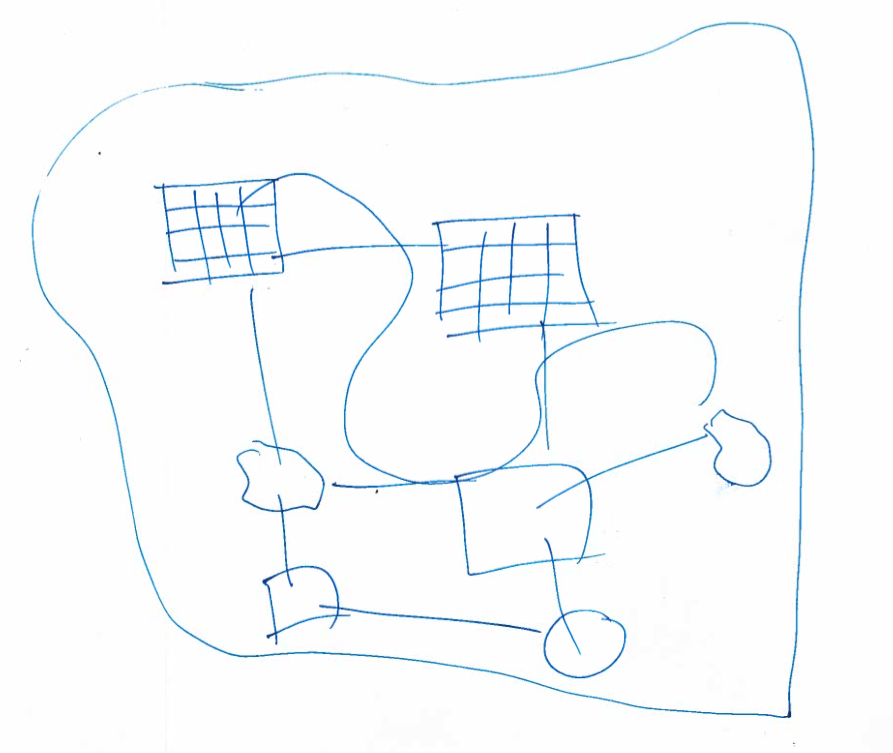
\includegraphics[width=6.5in]{interviews/drawings/2015_12_03.png}
\caption{\quotes{Interview 10 Software Engineer's drawing for `how you think of the code on this project?'}}
\end{figure}


\begin{figure}[H]
\centering
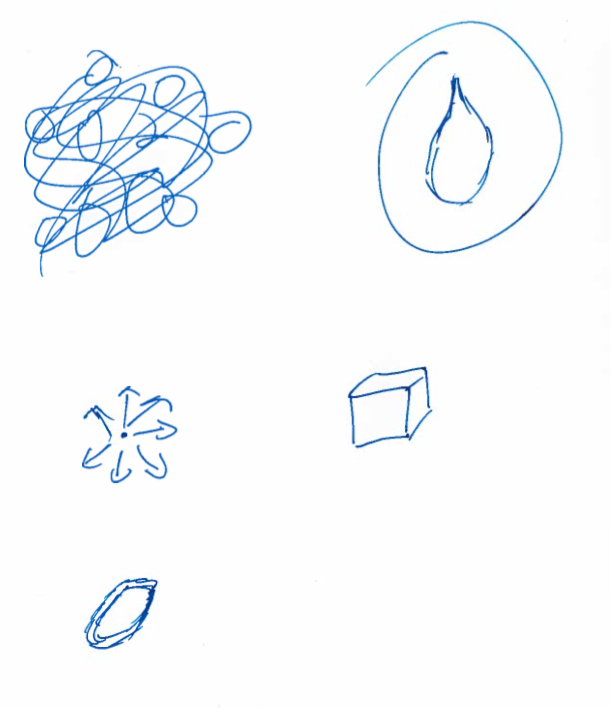
\includegraphics[width=6.5in]{interviews/drawings/2015_12_08.png}
\caption{\quotes{Interview 11: Software Engineer's drawing for `how you think about the code on this project?'}}
\end{figure}

\textbf{Interviewee 11:} It's kind of complicated. We have so many different pieces and this is what the connection feels like to me in my head where everything is jumbled together but at the same time, I do feel like the structure is clean but I'm having a hard time thinking of what to draw for like what represents clean. .  I'm just going to draw a water droplet to show that it looks clean.

It's more than just it's complicated, it's expanding a lot so in my head.  I'm thinking more like a big bang kind of thing where it starts out very small and now it just keeps expanding and growing and then we're adding a bunch of features. 

It's solid and clean. I feel like the project is very well tested so there's less chances of major breakings. It is solid. So I draw a rock cube.

Our codebase is pretty young, pretty flexible in ways that when we want to do refactors, it's not super complicated and not super hard to do. We are pretty good at like separating all the logic. It was really easy to do refactoring on the stuff that we want to do.  So, I guess it's pretty flexible of something flexible. So I draws a rubber band.

\begin{figure}[H]
\centering
\includegraphics[width=6.5in]{interviews/drawings/2015_12_10.png}
\caption{\quotes{Interview 13: Software Engineer's drawing for `how you think about the code on this project?'}}
\end{figure}


\begin{figure}[H]
\centering
\includegraphics[width=6.5in]{interviews/drawings/2016_01_14.png}
\caption{\quotes{Interview 17: Software Engineer's drawing for `How you feel or how you think about the code'}}
\end{figure}


\begin{figure}[H]
\centering
\includegraphics[width=6.5in]{interviews/drawings/2016_07_05a.png}
\caption{\quotes{Interview 25: Interaction Designer's drawing for `how you feel about your current product'}}
\end{figure}

\begin{figure}[H]
\centering
\includegraphics[width=6.5in]{interviews/drawings/2016_07_05b.png}
\caption{\quotes{Interview 25: Interaction Designer's drawing for `how you feel about your current product'}}
\end{figure}


\begin{figure}[H]
\centering
\includegraphics[width=6.5in]{interviews/drawings/2016_07_05_designer2.png}
\caption{\quotes{Interview 26: Interaction Designer's drawing for `How you feel or how you think about the code'}}
\end{figure}


\begin{figure}[H]
\centering
\includegraphics[width=6.5in]{interviews/drawings/2016_08_17.png}
\caption{\quotes{Interview 28: Software Engineer's drawing for `How you feel or how you think about the code'}}
\end{figure}

\begin{figure}[H]
\centering
\includegraphics[width=6.5in]{interviews/drawings/2016_08_18.png}
\caption{\quotes{Interview 29: Software Engineer's drawing for `How you feel or how you think about the code'}}
\end{figure}

\begin{figure}[H]
\centering
\includegraphics[width=6.5in]{interviews/drawings/2016_09_26.png}
\caption{\quotes{Interview 31: Software Engineer's drawing for `How you feel or how you think about the code'}}
\end{figure}

\begin{figure}[H]
\centering
\includegraphics[width=6.5in]{interviews/drawings/2016_09_26_engineer2.png}
\caption{\quotes{Interview 32: Software Engineer's drawing for `How you feel or how you think about the code'}}
\end{figure}


\begin{figure}[H]
\centering
\includegraphics[width=5.6in]{interviews/drawings/2016_09_29.png}
\caption{\quotes{Interview 33: Software Engineer's drawing for `How you feel or how you think about the code'}}
\end{figure}


\bibliographystyle{IEEEtran}
\bibliography{bibliography}

\backmatter


\end{document}